

\let\negmedspace\undefined
\let\negthickspace\undefined
\documentclass[journal,12pt,twocolumn]{IEEEtran}

%
\usepackage{setspace}
\usepackage{gensymb}
%\doublespacing
\singlespacing

%\usepackage{graphicx}
%\usepackage{amssymb}
%\usepackage{relsize}
\usepackage[cmex10]{amsmath}
%\usepackage{amsthm}
%\interdisplaylinepenalty=2500
%\savesymbol{iint}
%\usepackage{txfonts}
%\restoresymbol{TXF}{iint}
%\usepackage{wasysym}
\usepackage{amsthm}
%\usepackage{iithtlc}
\usepackage{mathrsfs}
\usepackage{txfonts}
\usepackage{stfloats}
\usepackage{steinmetz}
\usepackage{bm}
\usepackage{cite}
\usepackage{cases}
\usepackage{subfig}
%\usepackage{xtab}
\usepackage{longtable}
\usepackage{multirow}
%\usepackage{algorithm}
%\usepackage{algpseudocode}
\usepackage{enumitem}
\usepackage{mathtools}
\usepackage{tikz}
\usepackage{circuitikz}
\usepackage{verbatim}
\usepackage{tfrupee}
\usepackage[breaklinks=true]{hyperref}
%\usepackage{stmaryrd}
\usepackage{tkz-euclide} % loads  TikZ and tkz-base
%\usetkzobj{all}
\usepackage{listings}
    \usepackage{color}                                            %%
    \usepackage{array}                                            %%
    \usepackage{longtable}                                        %%
    \usepackage{calc}                                             %%
    \usepackage{multirow}                                         %%
    \usepackage{hhline}                                           %%
    \usepackage{ifthen}                                           %%
  %optionally (for landscape tables embedded in another document): %%
    \usepackage{lscape}     
\usepackage{multicol}
\usepackage{chngcntr}
%\usepackage{enumerate}

%\usepackage{wasysym}
%\newcounter{MYtempeqncnt}
\DeclareMathOperator*{\Res}{Res}
%\renewcommand{\baselinestretch}{2}
\renewcommand\thesection{\arabic{section}}
\renewcommand\thesubsection{\thesection.\arabic{subsection}}
\renewcommand\thesubsubsection{\thesubsection.\arabic{subsubsection}}

\renewcommand\thesectiondis{\arabic{section}}
\renewcommand\thesubsectiondis{\thesectiondis.\arabic{subsection}}
\renewcommand\thesubsubsectiondis{\thesubsectiondis.\arabic{subsubsection}}

% correct bad hyphenation here
\hyphenation{op-tical net-works semi-conduc-tor}
\def\inputGnumericTable{}                                 %%

\lstset{
%language=C,
frame=single, 
breaklines=true,
columns=fullflexible
}
%\lstset{
%language=tex,
%frame=single, 
%breaklines=true
%}

\begin{document}
%


\newtheorem{theorem}{Theorem}[section]
\newtheorem{problem}{Problem}
\newtheorem{proposition}{Proposition}[section]
\newtheorem{lemma}{Lemma}[section]
\newtheorem{corollary}[theorem]{Corollary}
\newtheorem{example}{Example}[section]
\newtheorem{definition}[problem]{Definition}
%\newtheorem{thm}{Theorem}[section] 
%\newtheorem{defn}[thm]{Definition}
%\newtheorem{algorithm}{Algorithm}[section]
%\newtheorem{cor}{Corollary}
\newcommand{\BEQA}{\begin{eqnarray}}
\newcommand{\EEQA}{\end{eqnarray}}
\newcommand{\define}{\stackrel{\triangle}{=}}

\bibliographystyle{IEEEtran}
%\bibliographystyle{ieeetr}


\providecommand{\mbf}{\mathbf}
\providecommand{\pr}[1]{\ensuremath{\Pr\left(#1\right)}}
\providecommand{\qfunc}[1]{\ensuremath{Q\left(#1\right)}}
\providecommand{\sbrak}[1]{\ensuremath{{}\left[#1\right]}}
\providecommand{\lsbrak}[1]{\ensuremath{{}\left[#1\right.}}
\providecommand{\rsbrak}[1]{\ensuremath{{}\left.#1\right]}}
\providecommand{\brak}[1]{\ensuremath{\left(#1\right)}}
\providecommand{\lbrak}[1]{\ensuremath{\left(#1\right.}}
\providecommand{\rbrak}[1]{\ensuremath{\left.#1\right)}}
\providecommand{\cbrak}[1]{\ensuremath{\left\{#1\right\}}}
\providecommand{\lcbrak}[1]{\ensuremath{\left\{#1\right.}}
\providecommand{\rcbrak}[1]{\ensuremath{\left.#1\right\}}}
\theoremstyle{remark}
\newtheorem{rem}{Remark}
\newcommand{\sgn}{\mathop{\mathrm{sgn}}}
\providecommand{\abs}[1]{\left\vert#1\right\vert}
\providecommand{\res}[1]{\Res\displaylimits_{#1}} 
\providecommand{\norm}[1]{\left\lVert#1\right\rVert}
%\providecommand{\norm}[1]{\lVert#1\rVert}
\providecommand{\mtx}[1]{\mathbf{#1}}
\providecommand{\mean}[1]{E\left[ #1 \right]}
\providecommand{\fourier}{\overset{\mathcal{F}}{ \rightleftharpoons}}
%\providecommand{\hilbert}{\overset{\mathcal{H}}{ \rightleftharpoons}}
\providecommand{\system}{\overset{\mathcal{H}}{ \longleftrightarrow}}
	%\newcommand{\solution}[2]{\textbf{Solution:}{#1}}
\newcommand{\solution}{\noindent \textbf{Solution: }}
\newcommand{\cosec}{\,\text{cosec}\,}
\providecommand{\dec}[2]{\ensuremath{\overset{#1}{\underset{#2}{\gtrless}}}}
\newcommand{\myvec}[1]{\ensuremath{\begin{pmatrix}#1\end{pmatrix}}}
\newcommand{\mydet}[1]{\ensuremath{\begin{vmatrix}#1\end{vmatrix}}}
%\numberwithin{equation}{section}
\numberwithin{equation}{subsection}
%\numberwithin{problem}{section}
%\numberwithin{definition}{section}
\makeatletter
\@addtoreset{figure}{problem}
\makeatother

\let\StandardTheFigure\thefigure
\let\vec\mathbf
%\renewcommand{\thefigure}{\theproblem.\arabic{figure}}
\renewcommand{\thefigure}{\theproblem}
%\setlist[enumerate,1]{before=\renewcommand\theequation{\theenumi.\arabic{equation}}
%\counterwithin{equation}{enumi}


%\renewcommand{\theequation}{\arabic{subsection}.\arabic{equation}}

\def\putbox#1#2#3{\makebox[0in][l]{\makebox[#1][l]{}\raisebox{\baselineskip}[0in][0in]{\raisebox{#2}[0in][0in]{#3}}}}
     \def\rightbox#1{\makebox[0in][r]{#1}}
     \def\centbox#1{\makebox[0in]{#1}}
     \def\topbox#1{\raisebox{-\baselineskip}[0in][0in]{#1}}
     \def\midbox#1{\raisebox{-0.5\baselineskip}[0in][0in]{#1}}

\vspace{3cm}

\title{
%	\logo{
Quadratic Forms
%	}
}
\author{ G V V Sharma$^{*}$% <-this % stops a space
	\thanks{*The author is with the Department
		of Electrical Engineering, Indian Institute of Technology, Hyderabad
		502285 India e-mail:  gadepall@iith.ac.in. All content in this manual is released under GNU GPL.  Free and open source.}
	
}	
%\title{
%	\logo{Matrix Analysis through Octave}{\begin{center}\includegraphics[scale=.24]{tlc}\end{center}}{}{HAMDSP}
%}


% paper title
% can use linebreaks \\ within to get better formatting as desired
%\title{Matrix Analysis through Octave}
%
%
% author names and IEEE memberships
% note positions of commas and nonbreaking spaces ( ~ ) LaTeX will not break
% a structure at a ~ so this keeps an author's name from being broken across
% two lines.
% use \thanks{} to gain access to the first footnote area
% a separate \thanks must be used for each paragraph as LaTeX2e's \thanks
% was not built to handle multiple paragraphs
%

%\author{<-this % stops a space
%\thanks{}}
%}
% note the % following the last \IEEEmembership and also \thanks - 
% these prevent an unwanted space from occurring between the last author name
% and the end of the author line. i.e., if you had this:
% 
% \author{....lastname \thanks{...} \thanks{...} }
%                     ^------------^------------^----Do not want these spaces!
%
% a space would be appended to the last name and could cause every name on that
% line to be shifted left slightly. This is one of those "LaTeX things". For
% instance, "\textbf{A} \textbf{B}" will typeset as "A B" not "AB". To get
% "AB" then you have to do: "\textbf{A}\textbf{B}"
% \thanks is no different in this regard, so shield the last } of each \thanks
% that ends a line with a % and do not let a space in before the next \thanks.
% Spaces after \IEEEmembership other than the last one are OK (and needed) as
% you are supposed to have spaces between the names. For what it is worth,
% this is a minor point as most people would not even notice if the said evil
% space somehow managed to creep in.



% The paper headers
%\markboth{Journal of \LaTeX\ Class Files,~Vol.~6, No.~1, January~2007}%
%{Shell \MakeLowercase{\textit{et al.}}: Bare Demo of IEEEtran.cls for Journals}
% The only time the second header will appear is for the odd numbered pages
% after the title page when using the twoside option.
% 
% *** Note that you probably will NOT want to include the author's ***
% *** name in the headers of peer review papers.                   ***
% You can use \ifCLASSOPTIONpeerreview for conditional compilation here if
% you desire.




% If you want to put a publisher's ID mark on the page you can do it like
% this:
%\IEEEpubid{0000--0000/00\$00.00~\copyright~2007 IEEE}
% Remember, if you use this you must call \IEEEpubidadjcol in the second
% column for its text to clear the IEEEpubid mark.



% make the title area
\maketitle

\newpage

\tableofcontents

\bigskip

\renewcommand{\thefigure}{\theenumi}
\renewcommand{\thetable}{\theenumi}
%\renewcommand{\theequation}{\theenumi}

%\begin{abstract}
%%\boldmath
%In this letter, an algorithm for evaluating the exact analytical bit error rate  (BER)  for the piecewise linear (PL) combiner for  multiple relays is presented. Previous results were available only for upto three relays. The algorithm is unique in the sense that  the actual mathematical expressions, that are prohibitively large, need not be explicitly obtained. The diversity gain due to multiple relays is shown through plots of the analytical BER, well supported by simulations. 
%
%\end{abstract}
% IEEEtran.cls defaults to using nonbold math in the Abstract.
% This preserves the distinction between vectors and scalars. However,
% if the journal you are submitting to favors bold math in the abstract,
% then you can use LaTeX's standard command \boldmath at the very start
% of the abstract to achieve this. Many IEEE journals frown on math
% in the abstract anyway.

% Note that keywords are not normally used for peerreview papers.
%\begin{IEEEkeywords}
%Cooperative diversity, decode and forward, piecewise linear
%\end{IEEEkeywords}



% For peer review papers, you can put extra information on the cover
% page as needed:
% \ifCLASSOPTIONpeerreview
% \begin{center} \bfseries EDICS Category: 3-BBND \end{center}
% \fi
%
% For peerreview papers, this IEEEtran command inserts a page break and
% creates the second title. It will be ignored for other modes.
%\IEEEpeerreviewmaketitle

\begin{abstract}
This book provides a computational approach to school geometry based on the NCERT textbooks from Class 6-12.  Links to sample Python codes are available in the text.  
\end{abstract}
Download python codes using 
\begin{lstlisting}
svn co https://github.com/gadepall/school/trunk/ncert/computation/codes
\end{lstlisting}

\section{Examples}
\renewcommand{\theequation}{\theenumi}
\begin{enumerate}[label=\thesection.\arabic*.,ref=\thesection.\theenumi]
\numberwithin{equation}{enumi}

%\renewcommand{\theequation}{\theenumi}
%\begin{enumerate}[label=\arabic*.,ref=\thesubsection.\theenumi]
%\numberwithin{equation}{enumi}
\item Find the equation of a circle with centre \myvec{-3\\2} and radius 4.
\\
\solution 
See Fig. 	\ref{fig:4.2.4_circle}.  The  general equation for the circle can be given as
\begin{align}
\vec{x}^T\vec{x} + 2\vec{O}^T\vec{x} +\norm{O}^2 - \vec{r}^2 &= 0
\end{align}
given equation of circle
\begin{align}
\vec{x}^T\vec{x} -25&= 0
\end{align} 
comparing bothe of equation we can find the value of r and value of  $\vec{O}$
\begin{align}
\vec{r}&= 4
\\
\vec{O} &= \myvec{0\\0}
\\
\implies \vec{B}-\vec{O} &= \myvec{-2.5\\3.5}
\\
\implies \norm{\vec{B} - \vec{O}}^2 &= 18.5 < 25
\\
\text{or, } OB < r&
\end{align} 
Hence, $\vec{B}$ lies inside the circle.

The following code plots Fig. 	\ref{fig:4.2.4_circle}

	\begin{lstlisting}
solutions/4/codes/circle/circle2.py
	\end{lstlisting}
\begin{figure}[!ht]
	\centering
	\includegraphics[width=\columnwidth]{./solutions/4/figures/circle/circle2.eps}
	\caption{circle }
	\label{fig:4.2.4_circle}
\end{figure}


\item Find the centre and radius of the circle
\begin{align}
\vec{x}^T\vec{x}+\myvec{8\\10}\vec{x} -8= 0
\end{align}
%
\\
\solution 
From theory, we understand that using dot product we can find the angle between the lines 
\begin{enumerate}
	\item 
	\begin{align}\label{eq:solutions/line_plane/74/codes:5}
		\frac{x-2}{2} = \frac{y-1}{5} &= \frac{z+3}{-3}, 
	\end{align}
	\begin{align}\label{eq:solutions/line_plane/74/codes:6}
		\frac{x+2}{-1} = \frac{y-4}{8} &= \frac{z-5}{4} 
	\end{align}


The above symmetric equations \ref{eq:solutions/line_plane/74/codes:5}, \ref{eq:solutions/line_plane/74/codes:6} can be represented in the vector form as 
\begin{align}\label{eq:solutions/line_plane/74/codes7}
	\quad \vec{r_1} &= \myvec{2\\1\\-3} + \lambda_1\myvec{2\\5\\-3}
	\\
	\quad \vec{r_2} &= \myvec{-2\\4\\5} + \lambda_2\myvec{-1\\8\\4}
\end{align}

As we have to find the angle between the vectors, we will only be taking the direction vectors into consideration. The direction vectors are $\vec{u}$ = $\myvec{2\\5\\-3}$ and $\vec{v}$ = $\myvec{-1\\8\\4}$. We can find the corresponding magnitude values

\begin{align}\label{eq:solutions/line_plane/74/codes9}
	\norm{\vec{u}} =\sqrt{2^{2}+5^{2}+(-3)^{2}} =\sqrt{38}
\end{align}
\begin{align}\label{eq:solutions/line_plane/74/codes10}
	\norm{\vec{v}} =\sqrt{(-1)^{2}+8^{2}+4^{2}} =\sqrt{81}
\end{align}

Using \ref{eq:solutions/line_plane/74/codes4}, \ref{eq:solutions/line_plane/74/codes9}, \ref{eq:solutions/line_plane/74/codes10} we get
\begin{align}
	\theta = \cos ^{-1}\frac{\myvec{2\\5\\-3}^{T}\myvec{-1\\8\\4}}{(\sqrt{38})(\sqrt{81})} 
	\\
	\theta = \cos ^{-1}\frac{26}{55.4797}
	\\
	\theta = \cos ^{-1} (0.4686)
	\\
	\theta = 62.053\degree
\end{align}

Therefore, the angle between the two lines is $62.053\degree$.See Fig. \ref{fig:solutions/line_plane/74/codesline_equation_1}

\begin{figure}
	\centering
	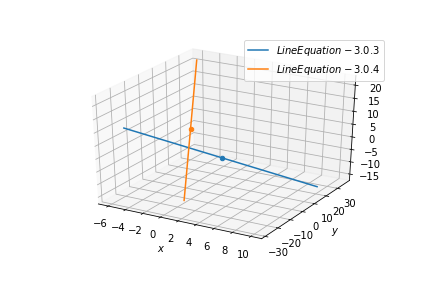
\includegraphics[width=\columnwidth]{./solutions/line_plane/74/codes/figs/Line_interest_1.png}
	\caption{Graph for equations \ref{eq:solutions/line_plane/74/codes7}}
	\label{fig:solutions/line_plane/74/codesline_equation_1}
\end{figure}


	\item 
	\begin{align}\label{eq:solutions/line_plane/74/codes12}
		\frac{x}{2} = \frac{y}{2} &= \frac{z}{1}, 
	\end{align}
	\begin{align}\label{eq:solutions/line_plane/74/codes13}
		\frac{x-5}{4} = \frac{y-2}{1} &= \frac{z-3}{8} 
	\end{align}



The above symmetric equations \ref{eq:solutions/line_plane/74/codes12}, \ref{eq:solutions/line_plane/74/codes13} can be represented in the vector form as 
\begin{align}\label{eq:solutions/line_plane/74/codes14}
	\quad \vec{r_1} &= \myvec{0\\0\\0} + \lambda_1\myvec{2\\2\\1}
	\\
	\quad \vec{r_2} &= \myvec{5\\2\\3} + \lambda_2\myvec{4\\1\\8}
\end{align}

As we have to find the angle between the vectors, we will only be taking the direction vectors into consideration. The direction vectors are $\vec{u}$ = $\myvec{2\\2\\1}$ and $\vec{v}$ = $\myvec{4\\1\\8}$. We can find the corresponding magnitude values

\begin{align}\label{eq:solutions/line_plane/74/codes16}
	\norm{\vec{u}} =\sqrt{2^{2}+2^{2}+1^{2}} =\sqrt{9}
\end{align}
\begin{align}\label{eq:solutions/line_plane/74/codes17}
	\norm{\vec{v}} =\sqrt{4^{2}+1^{2}+8^{2}} =\sqrt{81}
\end{align}

Using \ref{eq:solutions/line_plane/74/codes4}, \ref{eq:solutions/line_plane/74/codes16}, \ref{eq:solutions/line_plane/74/codes17} we get
\begin{align}
	\theta = \cos ^{-1}\frac{\myvec{2\\2\\1}^{T}\myvec{4\\1\\8}}{(\sqrt{9})(\sqrt{81})} 
	\\
	\theta = \cos ^{-1}\frac{18}{27.00}
	\\
	\theta = \cos ^{-1} (0.667)
	\\
	\theta = 48.189\degree
\end{align}

Therefore, the angle between the two lines is $48.189\degree$. See Fig. \ref{fig:solutions/line_plane/74/codesline_equation_2}


\begin{figure}
	\centering
	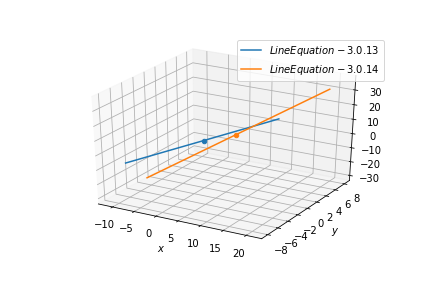
\includegraphics[width=\columnwidth]{./solutions/line_plane/74/codes/figs/Line_interest_2.png}
	\caption{Graph for equations \ref{eq:solutions/line_plane/74/codes14}}
	\label{fig:solutions/line_plane/74/codesline_equation_2}
\end{figure}
\end{enumerate}

    

\item Find the equation of the circle which passes through the points \myvec{2\\-2} and \myvec{3\\4} and whose centre lies on the line 
\begin{align}
\label{eq:4.1.3_line}
\myvec{1 & 1} \vec{x} = 2.
\end{align}
\\
\solution 
From theory, we understand that using dot product we can find the angle between the lines 
\begin{enumerate}
	\item 
	\begin{align}\label{eq:solutions/line_plane/74/codes:5}
		\frac{x-2}{2} = \frac{y-1}{5} &= \frac{z+3}{-3}, 
	\end{align}
	\begin{align}\label{eq:solutions/line_plane/74/codes:6}
		\frac{x+2}{-1} = \frac{y-4}{8} &= \frac{z-5}{4} 
	\end{align}


The above symmetric equations \ref{eq:solutions/line_plane/74/codes:5}, \ref{eq:solutions/line_plane/74/codes:6} can be represented in the vector form as 
\begin{align}\label{eq:solutions/line_plane/74/codes7}
	\quad \vec{r_1} &= \myvec{2\\1\\-3} + \lambda_1\myvec{2\\5\\-3}
	\\
	\quad \vec{r_2} &= \myvec{-2\\4\\5} + \lambda_2\myvec{-1\\8\\4}
\end{align}

As we have to find the angle between the vectors, we will only be taking the direction vectors into consideration. The direction vectors are $\vec{u}$ = $\myvec{2\\5\\-3}$ and $\vec{v}$ = $\myvec{-1\\8\\4}$. We can find the corresponding magnitude values

\begin{align}\label{eq:solutions/line_plane/74/codes9}
	\norm{\vec{u}} =\sqrt{2^{2}+5^{2}+(-3)^{2}} =\sqrt{38}
\end{align}
\begin{align}\label{eq:solutions/line_plane/74/codes10}
	\norm{\vec{v}} =\sqrt{(-1)^{2}+8^{2}+4^{2}} =\sqrt{81}
\end{align}

Using \ref{eq:solutions/line_plane/74/codes4}, \ref{eq:solutions/line_plane/74/codes9}, \ref{eq:solutions/line_plane/74/codes10} we get
\begin{align}
	\theta = \cos ^{-1}\frac{\myvec{2\\5\\-3}^{T}\myvec{-1\\8\\4}}{(\sqrt{38})(\sqrt{81})} 
	\\
	\theta = \cos ^{-1}\frac{26}{55.4797}
	\\
	\theta = \cos ^{-1} (0.4686)
	\\
	\theta = 62.053\degree
\end{align}

Therefore, the angle between the two lines is $62.053\degree$.See Fig. \ref{fig:solutions/line_plane/74/codesline_equation_1}

\begin{figure}
	\centering
	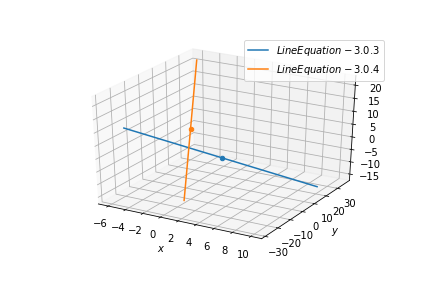
\includegraphics[width=\columnwidth]{./solutions/line_plane/74/codes/figs/Line_interest_1.png}
	\caption{Graph for equations \ref{eq:solutions/line_plane/74/codes7}}
	\label{fig:solutions/line_plane/74/codesline_equation_1}
\end{figure}


	\item 
	\begin{align}\label{eq:solutions/line_plane/74/codes12}
		\frac{x}{2} = \frac{y}{2} &= \frac{z}{1}, 
	\end{align}
	\begin{align}\label{eq:solutions/line_plane/74/codes13}
		\frac{x-5}{4} = \frac{y-2}{1} &= \frac{z-3}{8} 
	\end{align}



The above symmetric equations \ref{eq:solutions/line_plane/74/codes12}, \ref{eq:solutions/line_plane/74/codes13} can be represented in the vector form as 
\begin{align}\label{eq:solutions/line_plane/74/codes14}
	\quad \vec{r_1} &= \myvec{0\\0\\0} + \lambda_1\myvec{2\\2\\1}
	\\
	\quad \vec{r_2} &= \myvec{5\\2\\3} + \lambda_2\myvec{4\\1\\8}
\end{align}

As we have to find the angle between the vectors, we will only be taking the direction vectors into consideration. The direction vectors are $\vec{u}$ = $\myvec{2\\2\\1}$ and $\vec{v}$ = $\myvec{4\\1\\8}$. We can find the corresponding magnitude values

\begin{align}\label{eq:solutions/line_plane/74/codes16}
	\norm{\vec{u}} =\sqrt{2^{2}+2^{2}+1^{2}} =\sqrt{9}
\end{align}
\begin{align}\label{eq:solutions/line_plane/74/codes17}
	\norm{\vec{v}} =\sqrt{4^{2}+1^{2}+8^{2}} =\sqrt{81}
\end{align}

Using \ref{eq:solutions/line_plane/74/codes4}, \ref{eq:solutions/line_plane/74/codes16}, \ref{eq:solutions/line_plane/74/codes17} we get
\begin{align}
	\theta = \cos ^{-1}\frac{\myvec{2\\2\\1}^{T}\myvec{4\\1\\8}}{(\sqrt{9})(\sqrt{81})} 
	\\
	\theta = \cos ^{-1}\frac{18}{27.00}
	\\
	\theta = \cos ^{-1} (0.667)
	\\
	\theta = 48.189\degree
\end{align}

Therefore, the angle between the two lines is $48.189\degree$. See Fig. \ref{fig:solutions/line_plane/74/codesline_equation_2}


\begin{figure}
	\centering
	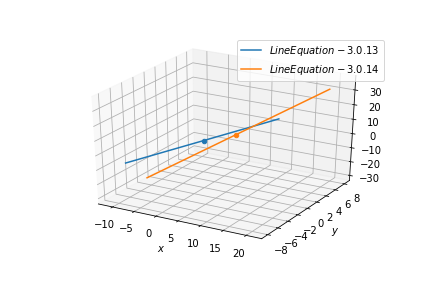
\includegraphics[width=\columnwidth]{./solutions/line_plane/74/codes/figs/Line_interest_2.png}
	\caption{Graph for equations \ref{eq:solutions/line_plane/74/codes14}}
	\label{fig:solutions/line_plane/74/codesline_equation_2}
\end{figure}
\end{enumerate}

    

\item Find the area enclosed by the circle $\norm{\vec{x}} = a$
%
\\
\solution The area is $2\pi a^2$.
%
\item Find the area of the region in the first quadrant enclosed by the x-axis, the line $\myvec{1 & -1}\vec{x} = 0$, and the circle $\norm{\vec{x}} = 1$.
%
\\
\solution 
From theory, we understand that using dot product we can find the angle between the lines 
\begin{enumerate}
	\item 
	\begin{align}\label{eq:solutions/line_plane/74/codes:5}
		\frac{x-2}{2} = \frac{y-1}{5} &= \frac{z+3}{-3}, 
	\end{align}
	\begin{align}\label{eq:solutions/line_plane/74/codes:6}
		\frac{x+2}{-1} = \frac{y-4}{8} &= \frac{z-5}{4} 
	\end{align}


The above symmetric equations \ref{eq:solutions/line_plane/74/codes:5}, \ref{eq:solutions/line_plane/74/codes:6} can be represented in the vector form as 
\begin{align}\label{eq:solutions/line_plane/74/codes7}
	\quad \vec{r_1} &= \myvec{2\\1\\-3} + \lambda_1\myvec{2\\5\\-3}
	\\
	\quad \vec{r_2} &= \myvec{-2\\4\\5} + \lambda_2\myvec{-1\\8\\4}
\end{align}

As we have to find the angle between the vectors, we will only be taking the direction vectors into consideration. The direction vectors are $\vec{u}$ = $\myvec{2\\5\\-3}$ and $\vec{v}$ = $\myvec{-1\\8\\4}$. We can find the corresponding magnitude values

\begin{align}\label{eq:solutions/line_plane/74/codes9}
	\norm{\vec{u}} =\sqrt{2^{2}+5^{2}+(-3)^{2}} =\sqrt{38}
\end{align}
\begin{align}\label{eq:solutions/line_plane/74/codes10}
	\norm{\vec{v}} =\sqrt{(-1)^{2}+8^{2}+4^{2}} =\sqrt{81}
\end{align}

Using \ref{eq:solutions/line_plane/74/codes4}, \ref{eq:solutions/line_plane/74/codes9}, \ref{eq:solutions/line_plane/74/codes10} we get
\begin{align}
	\theta = \cos ^{-1}\frac{\myvec{2\\5\\-3}^{T}\myvec{-1\\8\\4}}{(\sqrt{38})(\sqrt{81})} 
	\\
	\theta = \cos ^{-1}\frac{26}{55.4797}
	\\
	\theta = \cos ^{-1} (0.4686)
	\\
	\theta = 62.053\degree
\end{align}

Therefore, the angle between the two lines is $62.053\degree$.See Fig. \ref{fig:solutions/line_plane/74/codesline_equation_1}

\begin{figure}
	\centering
	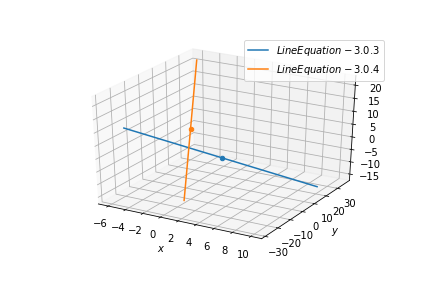
\includegraphics[width=\columnwidth]{./solutions/line_plane/74/codes/figs/Line_interest_1.png}
	\caption{Graph for equations \ref{eq:solutions/line_plane/74/codes7}}
	\label{fig:solutions/line_plane/74/codesline_equation_1}
\end{figure}


	\item 
	\begin{align}\label{eq:solutions/line_plane/74/codes12}
		\frac{x}{2} = \frac{y}{2} &= \frac{z}{1}, 
	\end{align}
	\begin{align}\label{eq:solutions/line_plane/74/codes13}
		\frac{x-5}{4} = \frac{y-2}{1} &= \frac{z-3}{8} 
	\end{align}



The above symmetric equations \ref{eq:solutions/line_plane/74/codes12}, \ref{eq:solutions/line_plane/74/codes13} can be represented in the vector form as 
\begin{align}\label{eq:solutions/line_plane/74/codes14}
	\quad \vec{r_1} &= \myvec{0\\0\\0} + \lambda_1\myvec{2\\2\\1}
	\\
	\quad \vec{r_2} &= \myvec{5\\2\\3} + \lambda_2\myvec{4\\1\\8}
\end{align}

As we have to find the angle between the vectors, we will only be taking the direction vectors into consideration. The direction vectors are $\vec{u}$ = $\myvec{2\\2\\1}$ and $\vec{v}$ = $\myvec{4\\1\\8}$. We can find the corresponding magnitude values

\begin{align}\label{eq:solutions/line_plane/74/codes16}
	\norm{\vec{u}} =\sqrt{2^{2}+2^{2}+1^{2}} =\sqrt{9}
\end{align}
\begin{align}\label{eq:solutions/line_plane/74/codes17}
	\norm{\vec{v}} =\sqrt{4^{2}+1^{2}+8^{2}} =\sqrt{81}
\end{align}

Using \ref{eq:solutions/line_plane/74/codes4}, \ref{eq:solutions/line_plane/74/codes16}, \ref{eq:solutions/line_plane/74/codes17} we get
\begin{align}
	\theta = \cos ^{-1}\frac{\myvec{2\\2\\1}^{T}\myvec{4\\1\\8}}{(\sqrt{9})(\sqrt{81})} 
	\\
	\theta = \cos ^{-1}\frac{18}{27.00}
	\\
	\theta = \cos ^{-1} (0.667)
	\\
	\theta = 48.189\degree
\end{align}

Therefore, the angle between the two lines is $48.189\degree$. See Fig. \ref{fig:solutions/line_plane/74/codesline_equation_2}


\begin{figure}
	\centering
	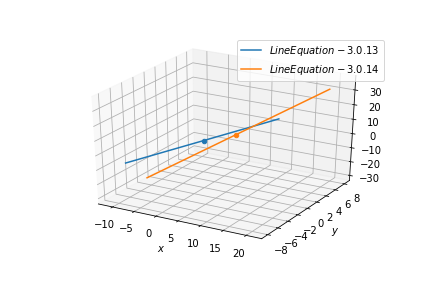
\includegraphics[width=\columnwidth]{./solutions/line_plane/74/codes/figs/Line_interest_2.png}
	\caption{Graph for equations \ref{eq:solutions/line_plane/74/codes14}}
	\label{fig:solutions/line_plane/74/codesline_equation_2}
\end{figure}
\end{enumerate}

    

%
\item Find the area of the region enclosed between the two circles: $\vec{x}^T\vec{x} = 4$ and $\norm{\vec{x}-\myvec{2\\0}} = 2$.
%
\item Find the coordinates of a point $\vec{A}$, where $AB$ is the diameter of a circle whose centre is \myvec{2,-3} and $\vec{B} = \myvec{1\\4}$.
\\
\solution 
From theory, we understand that using dot product we can find the angle between the lines 
\begin{enumerate}
	\item 
	\begin{align}\label{eq:solutions/line_plane/74/codes:5}
		\frac{x-2}{2} = \frac{y-1}{5} &= \frac{z+3}{-3}, 
	\end{align}
	\begin{align}\label{eq:solutions/line_plane/74/codes:6}
		\frac{x+2}{-1} = \frac{y-4}{8} &= \frac{z-5}{4} 
	\end{align}


The above symmetric equations \ref{eq:solutions/line_plane/74/codes:5}, \ref{eq:solutions/line_plane/74/codes:6} can be represented in the vector form as 
\begin{align}\label{eq:solutions/line_plane/74/codes7}
	\quad \vec{r_1} &= \myvec{2\\1\\-3} + \lambda_1\myvec{2\\5\\-3}
	\\
	\quad \vec{r_2} &= \myvec{-2\\4\\5} + \lambda_2\myvec{-1\\8\\4}
\end{align}

As we have to find the angle between the vectors, we will only be taking the direction vectors into consideration. The direction vectors are $\vec{u}$ = $\myvec{2\\5\\-3}$ and $\vec{v}$ = $\myvec{-1\\8\\4}$. We can find the corresponding magnitude values

\begin{align}\label{eq:solutions/line_plane/74/codes9}
	\norm{\vec{u}} =\sqrt{2^{2}+5^{2}+(-3)^{2}} =\sqrt{38}
\end{align}
\begin{align}\label{eq:solutions/line_plane/74/codes10}
	\norm{\vec{v}} =\sqrt{(-1)^{2}+8^{2}+4^{2}} =\sqrt{81}
\end{align}

Using \ref{eq:solutions/line_plane/74/codes4}, \ref{eq:solutions/line_plane/74/codes9}, \ref{eq:solutions/line_plane/74/codes10} we get
\begin{align}
	\theta = \cos ^{-1}\frac{\myvec{2\\5\\-3}^{T}\myvec{-1\\8\\4}}{(\sqrt{38})(\sqrt{81})} 
	\\
	\theta = \cos ^{-1}\frac{26}{55.4797}
	\\
	\theta = \cos ^{-1} (0.4686)
	\\
	\theta = 62.053\degree
\end{align}

Therefore, the angle between the two lines is $62.053\degree$.See Fig. \ref{fig:solutions/line_plane/74/codesline_equation_1}

\begin{figure}
	\centering
	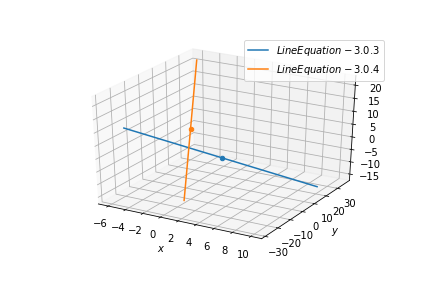
\includegraphics[width=\columnwidth]{./solutions/line_plane/74/codes/figs/Line_interest_1.png}
	\caption{Graph for equations \ref{eq:solutions/line_plane/74/codes7}}
	\label{fig:solutions/line_plane/74/codesline_equation_1}
\end{figure}


	\item 
	\begin{align}\label{eq:solutions/line_plane/74/codes12}
		\frac{x}{2} = \frac{y}{2} &= \frac{z}{1}, 
	\end{align}
	\begin{align}\label{eq:solutions/line_plane/74/codes13}
		\frac{x-5}{4} = \frac{y-2}{1} &= \frac{z-3}{8} 
	\end{align}



The above symmetric equations \ref{eq:solutions/line_plane/74/codes12}, \ref{eq:solutions/line_plane/74/codes13} can be represented in the vector form as 
\begin{align}\label{eq:solutions/line_plane/74/codes14}
	\quad \vec{r_1} &= \myvec{0\\0\\0} + \lambda_1\myvec{2\\2\\1}
	\\
	\quad \vec{r_2} &= \myvec{5\\2\\3} + \lambda_2\myvec{4\\1\\8}
\end{align}

As we have to find the angle between the vectors, we will only be taking the direction vectors into consideration. The direction vectors are $\vec{u}$ = $\myvec{2\\2\\1}$ and $\vec{v}$ = $\myvec{4\\1\\8}$. We can find the corresponding magnitude values

\begin{align}\label{eq:solutions/line_plane/74/codes16}
	\norm{\vec{u}} =\sqrt{2^{2}+2^{2}+1^{2}} =\sqrt{9}
\end{align}
\begin{align}\label{eq:solutions/line_plane/74/codes17}
	\norm{\vec{v}} =\sqrt{4^{2}+1^{2}+8^{2}} =\sqrt{81}
\end{align}

Using \ref{eq:solutions/line_plane/74/codes4}, \ref{eq:solutions/line_plane/74/codes16}, \ref{eq:solutions/line_plane/74/codes17} we get
\begin{align}
	\theta = \cos ^{-1}\frac{\myvec{2\\2\\1}^{T}\myvec{4\\1\\8}}{(\sqrt{9})(\sqrt{81})} 
	\\
	\theta = \cos ^{-1}\frac{18}{27.00}
	\\
	\theta = \cos ^{-1} (0.667)
	\\
	\theta = 48.189\degree
\end{align}

Therefore, the angle between the two lines is $48.189\degree$. See Fig. \ref{fig:solutions/line_plane/74/codesline_equation_2}


\begin{figure}
	\centering
	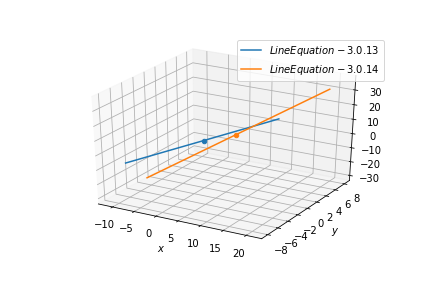
\includegraphics[width=\columnwidth]{./solutions/line_plane/74/codes/figs/Line_interest_2.png}
	\caption{Graph for equations \ref{eq:solutions/line_plane/74/codes14}}
	\label{fig:solutions/line_plane/74/codesline_equation_2}
\end{figure}
\end{enumerate}

    

\item Find the centre $O$ of a circle passing through the points \myvec{6\\-6}, \myvec{3\\-7} and  \myvec{3\\3}.
\solution 
From theory, we understand that using dot product we can find the angle between the lines 
\begin{enumerate}
	\item 
	\begin{align}\label{eq:solutions/line_plane/74/codes:5}
		\frac{x-2}{2} = \frac{y-1}{5} &= \frac{z+3}{-3}, 
	\end{align}
	\begin{align}\label{eq:solutions/line_plane/74/codes:6}
		\frac{x+2}{-1} = \frac{y-4}{8} &= \frac{z-5}{4} 
	\end{align}


The above symmetric equations \ref{eq:solutions/line_plane/74/codes:5}, \ref{eq:solutions/line_plane/74/codes:6} can be represented in the vector form as 
\begin{align}\label{eq:solutions/line_plane/74/codes7}
	\quad \vec{r_1} &= \myvec{2\\1\\-3} + \lambda_1\myvec{2\\5\\-3}
	\\
	\quad \vec{r_2} &= \myvec{-2\\4\\5} + \lambda_2\myvec{-1\\8\\4}
\end{align}

As we have to find the angle between the vectors, we will only be taking the direction vectors into consideration. The direction vectors are $\vec{u}$ = $\myvec{2\\5\\-3}$ and $\vec{v}$ = $\myvec{-1\\8\\4}$. We can find the corresponding magnitude values

\begin{align}\label{eq:solutions/line_plane/74/codes9}
	\norm{\vec{u}} =\sqrt{2^{2}+5^{2}+(-3)^{2}} =\sqrt{38}
\end{align}
\begin{align}\label{eq:solutions/line_plane/74/codes10}
	\norm{\vec{v}} =\sqrt{(-1)^{2}+8^{2}+4^{2}} =\sqrt{81}
\end{align}

Using \ref{eq:solutions/line_plane/74/codes4}, \ref{eq:solutions/line_plane/74/codes9}, \ref{eq:solutions/line_plane/74/codes10} we get
\begin{align}
	\theta = \cos ^{-1}\frac{\myvec{2\\5\\-3}^{T}\myvec{-1\\8\\4}}{(\sqrt{38})(\sqrt{81})} 
	\\
	\theta = \cos ^{-1}\frac{26}{55.4797}
	\\
	\theta = \cos ^{-1} (0.4686)
	\\
	\theta = 62.053\degree
\end{align}

Therefore, the angle between the two lines is $62.053\degree$.See Fig. \ref{fig:solutions/line_plane/74/codesline_equation_1}

\begin{figure}
	\centering
	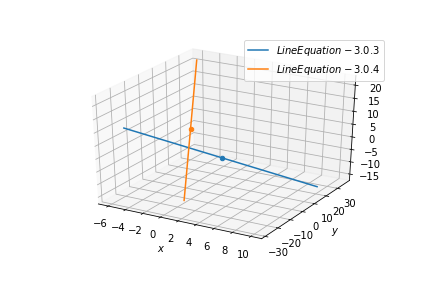
\includegraphics[width=\columnwidth]{./solutions/line_plane/74/codes/figs/Line_interest_1.png}
	\caption{Graph for equations \ref{eq:solutions/line_plane/74/codes7}}
	\label{fig:solutions/line_plane/74/codesline_equation_1}
\end{figure}


	\item 
	\begin{align}\label{eq:solutions/line_plane/74/codes12}
		\frac{x}{2} = \frac{y}{2} &= \frac{z}{1}, 
	\end{align}
	\begin{align}\label{eq:solutions/line_plane/74/codes13}
		\frac{x-5}{4} = \frac{y-2}{1} &= \frac{z-3}{8} 
	\end{align}



The above symmetric equations \ref{eq:solutions/line_plane/74/codes12}, \ref{eq:solutions/line_plane/74/codes13} can be represented in the vector form as 
\begin{align}\label{eq:solutions/line_plane/74/codes14}
	\quad \vec{r_1} &= \myvec{0\\0\\0} + \lambda_1\myvec{2\\2\\1}
	\\
	\quad \vec{r_2} &= \myvec{5\\2\\3} + \lambda_2\myvec{4\\1\\8}
\end{align}

As we have to find the angle between the vectors, we will only be taking the direction vectors into consideration. The direction vectors are $\vec{u}$ = $\myvec{2\\2\\1}$ and $\vec{v}$ = $\myvec{4\\1\\8}$. We can find the corresponding magnitude values

\begin{align}\label{eq:solutions/line_plane/74/codes16}
	\norm{\vec{u}} =\sqrt{2^{2}+2^{2}+1^{2}} =\sqrt{9}
\end{align}
\begin{align}\label{eq:solutions/line_plane/74/codes17}
	\norm{\vec{v}} =\sqrt{4^{2}+1^{2}+8^{2}} =\sqrt{81}
\end{align}

Using \ref{eq:solutions/line_plane/74/codes4}, \ref{eq:solutions/line_plane/74/codes16}, \ref{eq:solutions/line_plane/74/codes17} we get
\begin{align}
	\theta = \cos ^{-1}\frac{\myvec{2\\2\\1}^{T}\myvec{4\\1\\8}}{(\sqrt{9})(\sqrt{81})} 
	\\
	\theta = \cos ^{-1}\frac{18}{27.00}
	\\
	\theta = \cos ^{-1} (0.667)
	\\
	\theta = 48.189\degree
\end{align}

Therefore, the angle between the two lines is $48.189\degree$. See Fig. \ref{fig:solutions/line_plane/74/codesline_equation_2}


\begin{figure}
	\centering
	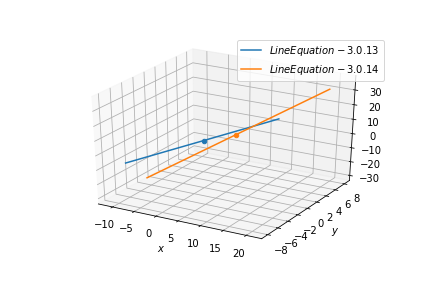
\includegraphics[width=\columnwidth]{./solutions/line_plane/74/codes/figs/Line_interest_2.png}
	\caption{Graph for equations \ref{eq:solutions/line_plane/74/codes14}}
	\label{fig:solutions/line_plane/74/codesline_equation_2}
\end{figure}
\end{enumerate}

    

\item Sketch the circles with 
\begin{enumerate}
\item centre \myvec{0\\2} and radius 2
\item centre \myvec{-2\\32} and radius 4
\item centre $\myvec{\frac{1}{2}\\ \frac{1}{4}}$ and radius $\frac{1}{12}$.
\item centre \myvec{1\\1} and radius $\sqrt{2}$.
\item centre \myvec{-a\\-b} and radius $\sqrt{a^2-b^2}$.
\end{enumerate}
\solution 
From theory, we understand that using dot product we can find the angle between the lines 
\begin{enumerate}
	\item 
	\begin{align}\label{eq:solutions/line_plane/74/codes:5}
		\frac{x-2}{2} = \frac{y-1}{5} &= \frac{z+3}{-3}, 
	\end{align}
	\begin{align}\label{eq:solutions/line_plane/74/codes:6}
		\frac{x+2}{-1} = \frac{y-4}{8} &= \frac{z-5}{4} 
	\end{align}


The above symmetric equations \ref{eq:solutions/line_plane/74/codes:5}, \ref{eq:solutions/line_plane/74/codes:6} can be represented in the vector form as 
\begin{align}\label{eq:solutions/line_plane/74/codes7}
	\quad \vec{r_1} &= \myvec{2\\1\\-3} + \lambda_1\myvec{2\\5\\-3}
	\\
	\quad \vec{r_2} &= \myvec{-2\\4\\5} + \lambda_2\myvec{-1\\8\\4}
\end{align}

As we have to find the angle between the vectors, we will only be taking the direction vectors into consideration. The direction vectors are $\vec{u}$ = $\myvec{2\\5\\-3}$ and $\vec{v}$ = $\myvec{-1\\8\\4}$. We can find the corresponding magnitude values

\begin{align}\label{eq:solutions/line_plane/74/codes9}
	\norm{\vec{u}} =\sqrt{2^{2}+5^{2}+(-3)^{2}} =\sqrt{38}
\end{align}
\begin{align}\label{eq:solutions/line_plane/74/codes10}
	\norm{\vec{v}} =\sqrt{(-1)^{2}+8^{2}+4^{2}} =\sqrt{81}
\end{align}

Using \ref{eq:solutions/line_plane/74/codes4}, \ref{eq:solutions/line_plane/74/codes9}, \ref{eq:solutions/line_plane/74/codes10} we get
\begin{align}
	\theta = \cos ^{-1}\frac{\myvec{2\\5\\-3}^{T}\myvec{-1\\8\\4}}{(\sqrt{38})(\sqrt{81})} 
	\\
	\theta = \cos ^{-1}\frac{26}{55.4797}
	\\
	\theta = \cos ^{-1} (0.4686)
	\\
	\theta = 62.053\degree
\end{align}

Therefore, the angle between the two lines is $62.053\degree$.See Fig. \ref{fig:solutions/line_plane/74/codesline_equation_1}

\begin{figure}
	\centering
	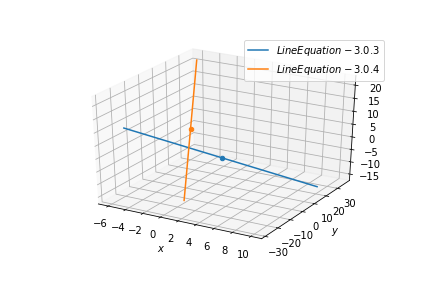
\includegraphics[width=\columnwidth]{./solutions/line_plane/74/codes/figs/Line_interest_1.png}
	\caption{Graph for equations \ref{eq:solutions/line_plane/74/codes7}}
	\label{fig:solutions/line_plane/74/codesline_equation_1}
\end{figure}


	\item 
	\begin{align}\label{eq:solutions/line_plane/74/codes12}
		\frac{x}{2} = \frac{y}{2} &= \frac{z}{1}, 
	\end{align}
	\begin{align}\label{eq:solutions/line_plane/74/codes13}
		\frac{x-5}{4} = \frac{y-2}{1} &= \frac{z-3}{8} 
	\end{align}



The above symmetric equations \ref{eq:solutions/line_plane/74/codes12}, \ref{eq:solutions/line_plane/74/codes13} can be represented in the vector form as 
\begin{align}\label{eq:solutions/line_plane/74/codes14}
	\quad \vec{r_1} &= \myvec{0\\0\\0} + \lambda_1\myvec{2\\2\\1}
	\\
	\quad \vec{r_2} &= \myvec{5\\2\\3} + \lambda_2\myvec{4\\1\\8}
\end{align}

As we have to find the angle between the vectors, we will only be taking the direction vectors into consideration. The direction vectors are $\vec{u}$ = $\myvec{2\\2\\1}$ and $\vec{v}$ = $\myvec{4\\1\\8}$. We can find the corresponding magnitude values

\begin{align}\label{eq:solutions/line_plane/74/codes16}
	\norm{\vec{u}} =\sqrt{2^{2}+2^{2}+1^{2}} =\sqrt{9}
\end{align}
\begin{align}\label{eq:solutions/line_plane/74/codes17}
	\norm{\vec{v}} =\sqrt{4^{2}+1^{2}+8^{2}} =\sqrt{81}
\end{align}

Using \ref{eq:solutions/line_plane/74/codes4}, \ref{eq:solutions/line_plane/74/codes16}, \ref{eq:solutions/line_plane/74/codes17} we get
\begin{align}
	\theta = \cos ^{-1}\frac{\myvec{2\\2\\1}^{T}\myvec{4\\1\\8}}{(\sqrt{9})(\sqrt{81})} 
	\\
	\theta = \cos ^{-1}\frac{18}{27.00}
	\\
	\theta = \cos ^{-1} (0.667)
	\\
	\theta = 48.189\degree
\end{align}

Therefore, the angle between the two lines is $48.189\degree$. See Fig. \ref{fig:solutions/line_plane/74/codesline_equation_2}


\begin{figure}
	\centering
	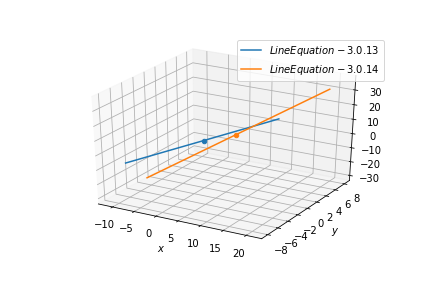
\includegraphics[width=\columnwidth]{./solutions/line_plane/74/codes/figs/Line_interest_2.png}
	\caption{Graph for equations \ref{eq:solutions/line_plane/74/codes14}}
	\label{fig:solutions/line_plane/74/codesline_equation_2}
\end{figure}
\end{enumerate}

    

\item  Does the point \myvec{–2.5\\ 3.5} lie inside, outside or on the circle $\vec{x}^T\vec{x} = 25$?
\\
\solution 
See Fig. 	\ref{fig:4.2.4_circle}.  The  general equation for the circle can be given as
\begin{align}
\vec{x}^T\vec{x} + 2\vec{O}^T\vec{x} +\norm{O}^2 - \vec{r}^2 &= 0
\end{align}
given equation of circle
\begin{align}
\vec{x}^T\vec{x} -25&= 0
\end{align} 
comparing bothe of equation we can find the value of r and value of  $\vec{O}$
\begin{align}
\vec{r}&= 4
\\
\vec{O} &= \myvec{0\\0}
\\
\implies \vec{B}-\vec{O} &= \myvec{-2.5\\3.5}
\\
\implies \norm{\vec{B} - \vec{O}}^2 &= 18.5 < 25
\\
\text{or, } OB < r&
\end{align} 
Hence, $\vec{B}$ lies inside the circle.

The following code plots Fig. 	\ref{fig:4.2.4_circle}

	\begin{lstlisting}
solutions/4/codes/circle/circle2.py
	\end{lstlisting}
\begin{figure}[!ht]
	\centering
	\includegraphics[width=\columnwidth]{./solutions/4/figures/circle/circle2.eps}
	\caption{circle }
	\label{fig:4.2.4_circle}
\end{figure}

\item Sketch the circles with equation
\begin{enumerate}
\item $\norm{\vec{x}-\myvec{5\\-3}}^2 = 36$
\item $\vec{x}^T\vec{x}-\myvec{4\\8}\vec{x} -45= 0$
\item $\vec{x}^T\vec{x}-\myvec{8\\-10}\vec{x} -12= 0$
\item $2\vec{x}^T\vec{x}-\myvec{1\\0}\vec{x} = 0$
\end{enumerate}
\solution 
The following python codes generate the required circle
	\begin{lstlisting}
	./solutions/5/codes/circle/q18abc.py
	./solutions/5/codes/circle/q18d.py
	\end{lstlisting}


\begin{enumerate}

\item \begin{align} 
\vec{x^Tx} - \myvec{4\\8}\vec{x} -45 = 0
\end{align}
See Fig. \ref{fig:4.2.5_qoeabc}.
\begin{align}
\vec{O} = \myvec{2\\4}, r = \sqrt{65} 
\end{align}
	\begin{figure}[!ht]
	\centering
	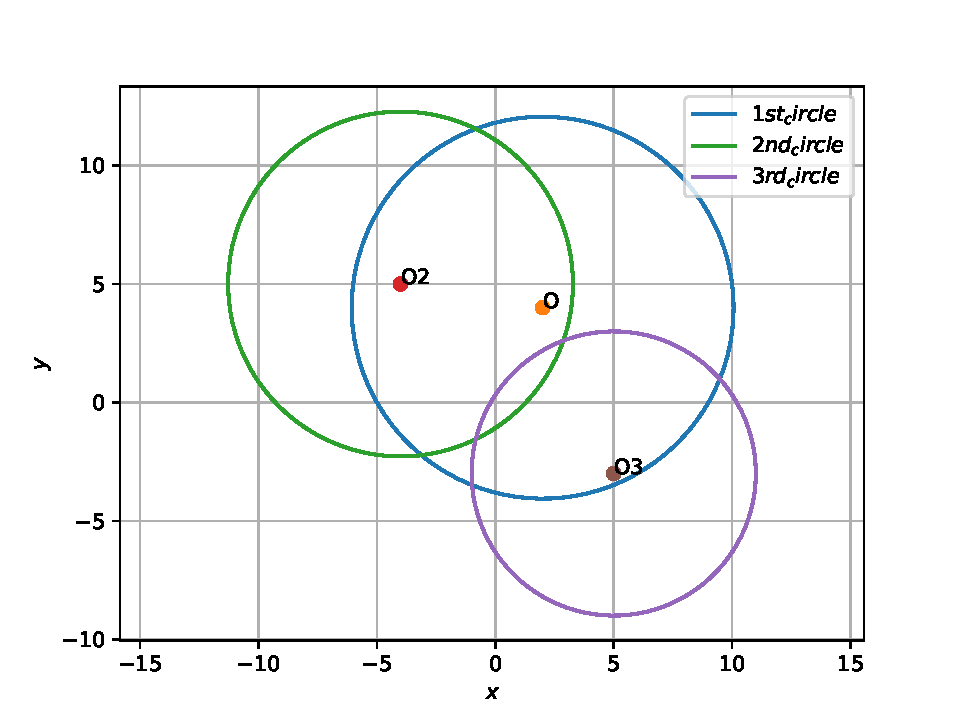
\includegraphics[width=\columnwidth]{./solutions/5/figs/circle/q18abc.eps}
	\caption{}
	\label{fig:4.2.5_qoeabc}	
	\end{figure}

\item See Fig. \ref{fig:4.2.5_qoeabc}.
\begin{align}
\vec{O} = \myvec{-4\\5}, r = \sqrt{53} 
\end{align}

\begin{align} 
\vec{x^Tx} - \myvec{8\\-10}\vec{x} - 12 = 0
\end{align}


\item See Fig. \ref{fig:4.2.5_qoeabc}.
\begin{align}
\vec{O} = \myvec{5\\-3}, r = 6
\end{align}
\begin{align} 
\norm{x - \myvec{5\\-3}} = 36
\end{align}



\begin{comment}
	\begin{figure}[!ht]
	\centering
	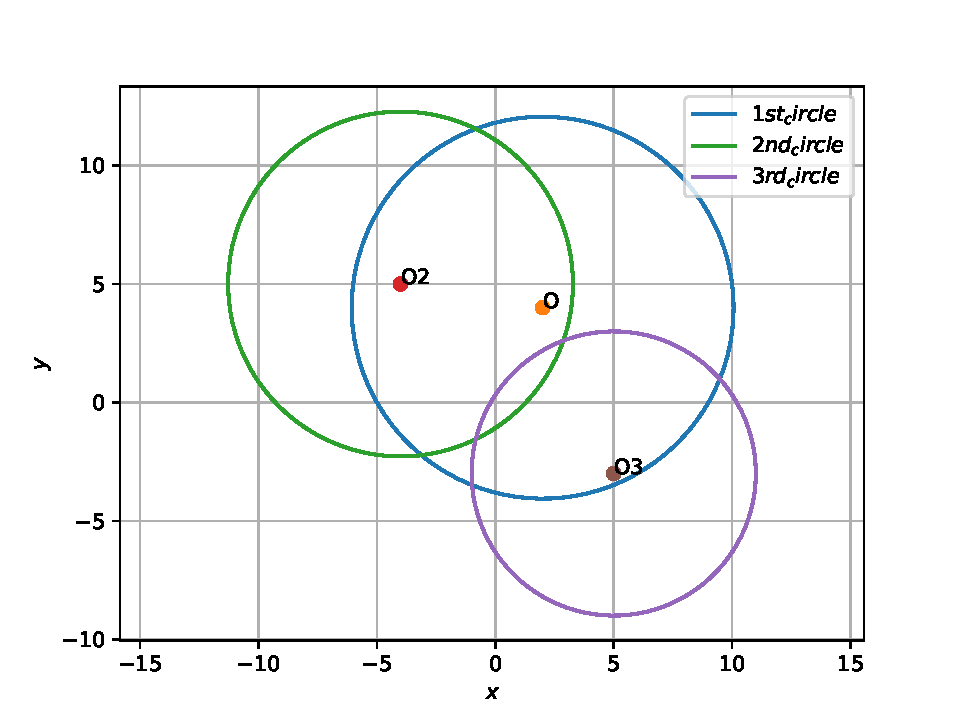
\includegraphics[width=\columnwidth]{./solutions/5/figs/circle/q18abc.eps}
	\caption{Circle of Q.4.2.5}
	\label{fig:4.2.5_qoeb}	
	\end{figure}
\end{comment}
\begin{comment}
	\begin{figure}[!ht]
	\centering
	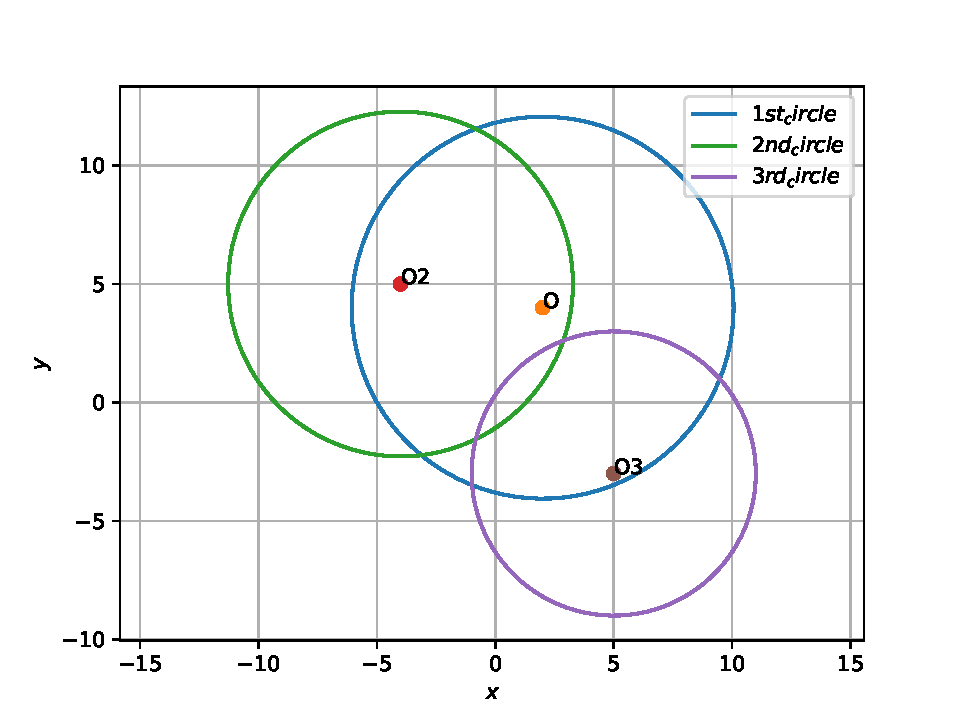
\includegraphics[width=\columnwidth]{./solutions/5/figs/circle/q18abc.eps}
	\caption{Circle of Q.4.2.5}
	\label{fig:4.2.5_qoec}	
	\end{figure}
\end{comment}
\item See Fig. \ref{fig:4.2.5_qoed}.
\begin{align}
\vec{O} = \frac{1}{4}\myvec{1\\0}, r = \frac{1}{4}
\end{align}
\begin{align} 
2\vec{x^Tx} - \myvec{1\\0}\vec{x} = 0
\end{align}
	\begin{figure}[!ht]
	\centering
	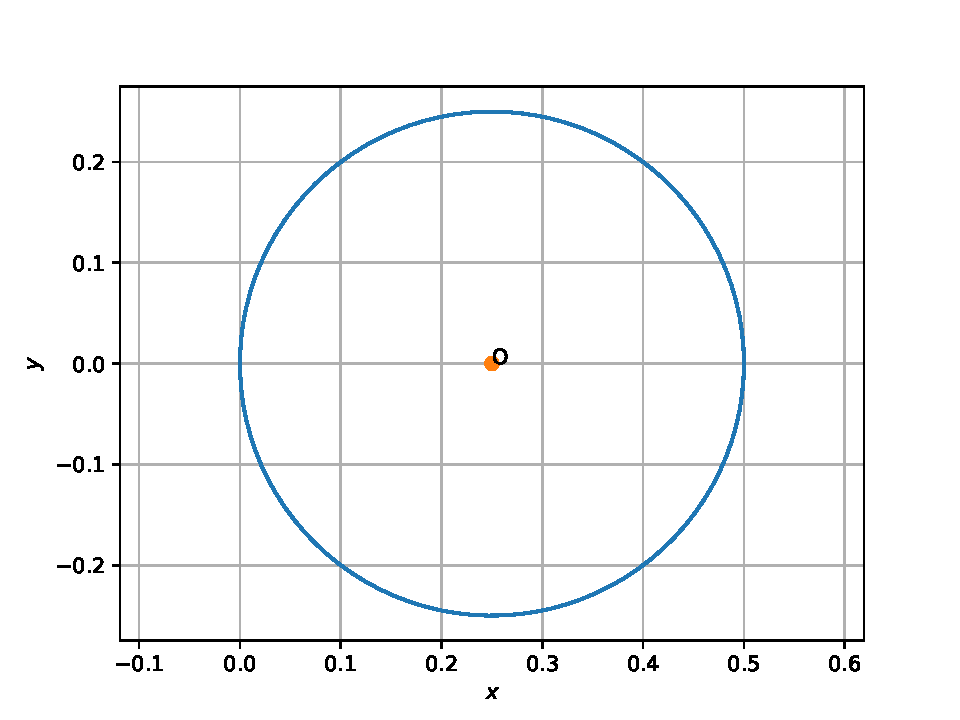
\includegraphics[width=\columnwidth]{./solutions/5/figs/circle/q18d.eps}
	\caption{}
	\label{fig:4.2.5_qoed}	
	\end{figure}



\end{enumerate}

\item Find the equation of the circle passing through the points \myvec{4\\1} and \myvec{6\\5} and whose centre is on the line $\myvec{4 & 1}\vec{x} = 16$.
\\
\solution 
From theory, we understand that using dot product we can find the angle between the lines 
\begin{enumerate}
	\item 
	\begin{align}\label{eq:solutions/line_plane/74/codes:5}
		\frac{x-2}{2} = \frac{y-1}{5} &= \frac{z+3}{-3}, 
	\end{align}
	\begin{align}\label{eq:solutions/line_plane/74/codes:6}
		\frac{x+2}{-1} = \frac{y-4}{8} &= \frac{z-5}{4} 
	\end{align}


The above symmetric equations \ref{eq:solutions/line_plane/74/codes:5}, \ref{eq:solutions/line_plane/74/codes:6} can be represented in the vector form as 
\begin{align}\label{eq:solutions/line_plane/74/codes7}
	\quad \vec{r_1} &= \myvec{2\\1\\-3} + \lambda_1\myvec{2\\5\\-3}
	\\
	\quad \vec{r_2} &= \myvec{-2\\4\\5} + \lambda_2\myvec{-1\\8\\4}
\end{align}

As we have to find the angle between the vectors, we will only be taking the direction vectors into consideration. The direction vectors are $\vec{u}$ = $\myvec{2\\5\\-3}$ and $\vec{v}$ = $\myvec{-1\\8\\4}$. We can find the corresponding magnitude values

\begin{align}\label{eq:solutions/line_plane/74/codes9}
	\norm{\vec{u}} =\sqrt{2^{2}+5^{2}+(-3)^{2}} =\sqrt{38}
\end{align}
\begin{align}\label{eq:solutions/line_plane/74/codes10}
	\norm{\vec{v}} =\sqrt{(-1)^{2}+8^{2}+4^{2}} =\sqrt{81}
\end{align}

Using \ref{eq:solutions/line_plane/74/codes4}, \ref{eq:solutions/line_plane/74/codes9}, \ref{eq:solutions/line_plane/74/codes10} we get
\begin{align}
	\theta = \cos ^{-1}\frac{\myvec{2\\5\\-3}^{T}\myvec{-1\\8\\4}}{(\sqrt{38})(\sqrt{81})} 
	\\
	\theta = \cos ^{-1}\frac{26}{55.4797}
	\\
	\theta = \cos ^{-1} (0.4686)
	\\
	\theta = 62.053\degree
\end{align}

Therefore, the angle between the two lines is $62.053\degree$.See Fig. \ref{fig:solutions/line_plane/74/codesline_equation_1}

\begin{figure}
	\centering
	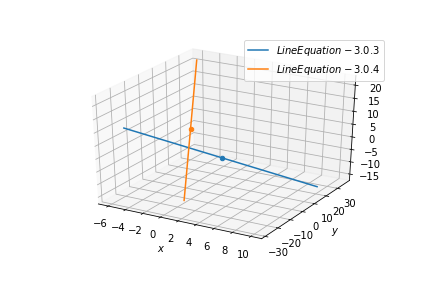
\includegraphics[width=\columnwidth]{./solutions/line_plane/74/codes/figs/Line_interest_1.png}
	\caption{Graph for equations \ref{eq:solutions/line_plane/74/codes7}}
	\label{fig:solutions/line_plane/74/codesline_equation_1}
\end{figure}


	\item 
	\begin{align}\label{eq:solutions/line_plane/74/codes12}
		\frac{x}{2} = \frac{y}{2} &= \frac{z}{1}, 
	\end{align}
	\begin{align}\label{eq:solutions/line_plane/74/codes13}
		\frac{x-5}{4} = \frac{y-2}{1} &= \frac{z-3}{8} 
	\end{align}



The above symmetric equations \ref{eq:solutions/line_plane/74/codes12}, \ref{eq:solutions/line_plane/74/codes13} can be represented in the vector form as 
\begin{align}\label{eq:solutions/line_plane/74/codes14}
	\quad \vec{r_1} &= \myvec{0\\0\\0} + \lambda_1\myvec{2\\2\\1}
	\\
	\quad \vec{r_2} &= \myvec{5\\2\\3} + \lambda_2\myvec{4\\1\\8}
\end{align}

As we have to find the angle between the vectors, we will only be taking the direction vectors into consideration. The direction vectors are $\vec{u}$ = $\myvec{2\\2\\1}$ and $\vec{v}$ = $\myvec{4\\1\\8}$. We can find the corresponding magnitude values

\begin{align}\label{eq:solutions/line_plane/74/codes16}
	\norm{\vec{u}} =\sqrt{2^{2}+2^{2}+1^{2}} =\sqrt{9}
\end{align}
\begin{align}\label{eq:solutions/line_plane/74/codes17}
	\norm{\vec{v}} =\sqrt{4^{2}+1^{2}+8^{2}} =\sqrt{81}
\end{align}

Using \ref{eq:solutions/line_plane/74/codes4}, \ref{eq:solutions/line_plane/74/codes16}, \ref{eq:solutions/line_plane/74/codes17} we get
\begin{align}
	\theta = \cos ^{-1}\frac{\myvec{2\\2\\1}^{T}\myvec{4\\1\\8}}{(\sqrt{9})(\sqrt{81})} 
	\\
	\theta = \cos ^{-1}\frac{18}{27.00}
	\\
	\theta = \cos ^{-1} (0.667)
	\\
	\theta = 48.189\degree
\end{align}

Therefore, the angle between the two lines is $48.189\degree$. See Fig. \ref{fig:solutions/line_plane/74/codesline_equation_2}


\begin{figure}
	\centering
	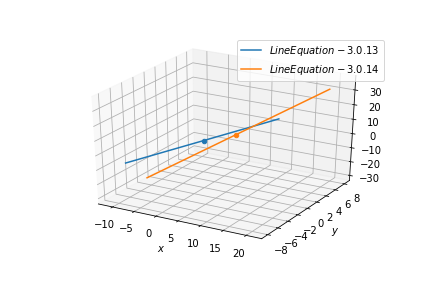
\includegraphics[width=\columnwidth]{./solutions/line_plane/74/codes/figs/Line_interest_2.png}
	\caption{Graph for equations \ref{eq:solutions/line_plane/74/codes14}}
	\label{fig:solutions/line_plane/74/codesline_equation_2}
\end{figure}
\end{enumerate}

    

\item Find the equation of the circle passing through the points $\vec{P} =\myvec{2\\3}$ and $\vec{Q} = \myvec{–1\\1}$ and whose centre is on the line $\myvec{1 & -3}\vec{x} = 11$.
\solution 
From theory, we understand that using dot product we can find the angle between the lines 
\begin{enumerate}
	\item 
	\begin{align}\label{eq:solutions/line_plane/74/codes:5}
		\frac{x-2}{2} = \frac{y-1}{5} &= \frac{z+3}{-3}, 
	\end{align}
	\begin{align}\label{eq:solutions/line_plane/74/codes:6}
		\frac{x+2}{-1} = \frac{y-4}{8} &= \frac{z-5}{4} 
	\end{align}


The above symmetric equations \ref{eq:solutions/line_plane/74/codes:5}, \ref{eq:solutions/line_plane/74/codes:6} can be represented in the vector form as 
\begin{align}\label{eq:solutions/line_plane/74/codes7}
	\quad \vec{r_1} &= \myvec{2\\1\\-3} + \lambda_1\myvec{2\\5\\-3}
	\\
	\quad \vec{r_2} &= \myvec{-2\\4\\5} + \lambda_2\myvec{-1\\8\\4}
\end{align}

As we have to find the angle between the vectors, we will only be taking the direction vectors into consideration. The direction vectors are $\vec{u}$ = $\myvec{2\\5\\-3}$ and $\vec{v}$ = $\myvec{-1\\8\\4}$. We can find the corresponding magnitude values

\begin{align}\label{eq:solutions/line_plane/74/codes9}
	\norm{\vec{u}} =\sqrt{2^{2}+5^{2}+(-3)^{2}} =\sqrt{38}
\end{align}
\begin{align}\label{eq:solutions/line_plane/74/codes10}
	\norm{\vec{v}} =\sqrt{(-1)^{2}+8^{2}+4^{2}} =\sqrt{81}
\end{align}

Using \ref{eq:solutions/line_plane/74/codes4}, \ref{eq:solutions/line_plane/74/codes9}, \ref{eq:solutions/line_plane/74/codes10} we get
\begin{align}
	\theta = \cos ^{-1}\frac{\myvec{2\\5\\-3}^{T}\myvec{-1\\8\\4}}{(\sqrt{38})(\sqrt{81})} 
	\\
	\theta = \cos ^{-1}\frac{26}{55.4797}
	\\
	\theta = \cos ^{-1} (0.4686)
	\\
	\theta = 62.053\degree
\end{align}

Therefore, the angle between the two lines is $62.053\degree$.See Fig. \ref{fig:solutions/line_plane/74/codesline_equation_1}

\begin{figure}
	\centering
	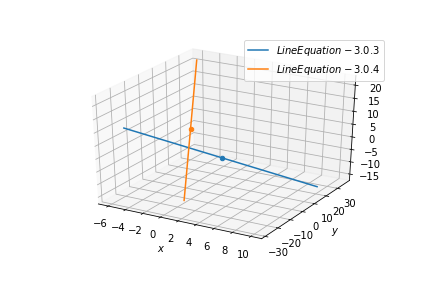
\includegraphics[width=\columnwidth]{./solutions/line_plane/74/codes/figs/Line_interest_1.png}
	\caption{Graph for equations \ref{eq:solutions/line_plane/74/codes7}}
	\label{fig:solutions/line_plane/74/codesline_equation_1}
\end{figure}


	\item 
	\begin{align}\label{eq:solutions/line_plane/74/codes12}
		\frac{x}{2} = \frac{y}{2} &= \frac{z}{1}, 
	\end{align}
	\begin{align}\label{eq:solutions/line_plane/74/codes13}
		\frac{x-5}{4} = \frac{y-2}{1} &= \frac{z-3}{8} 
	\end{align}



The above symmetric equations \ref{eq:solutions/line_plane/74/codes12}, \ref{eq:solutions/line_plane/74/codes13} can be represented in the vector form as 
\begin{align}\label{eq:solutions/line_plane/74/codes14}
	\quad \vec{r_1} &= \myvec{0\\0\\0} + \lambda_1\myvec{2\\2\\1}
	\\
	\quad \vec{r_2} &= \myvec{5\\2\\3} + \lambda_2\myvec{4\\1\\8}
\end{align}

As we have to find the angle between the vectors, we will only be taking the direction vectors into consideration. The direction vectors are $\vec{u}$ = $\myvec{2\\2\\1}$ and $\vec{v}$ = $\myvec{4\\1\\8}$. We can find the corresponding magnitude values

\begin{align}\label{eq:solutions/line_plane/74/codes16}
	\norm{\vec{u}} =\sqrt{2^{2}+2^{2}+1^{2}} =\sqrt{9}
\end{align}
\begin{align}\label{eq:solutions/line_plane/74/codes17}
	\norm{\vec{v}} =\sqrt{4^{2}+1^{2}+8^{2}} =\sqrt{81}
\end{align}

Using \ref{eq:solutions/line_plane/74/codes4}, \ref{eq:solutions/line_plane/74/codes16}, \ref{eq:solutions/line_plane/74/codes17} we get
\begin{align}
	\theta = \cos ^{-1}\frac{\myvec{2\\2\\1}^{T}\myvec{4\\1\\8}}{(\sqrt{9})(\sqrt{81})} 
	\\
	\theta = \cos ^{-1}\frac{18}{27.00}
	\\
	\theta = \cos ^{-1} (0.667)
	\\
	\theta = 48.189\degree
\end{align}

Therefore, the angle between the two lines is $48.189\degree$. See Fig. \ref{fig:solutions/line_plane/74/codesline_equation_2}


\begin{figure}
	\centering
	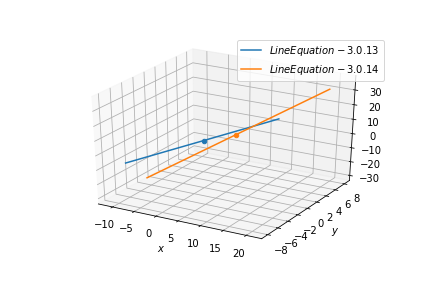
\includegraphics[width=\columnwidth]{./solutions/line_plane/74/codes/figs/Line_interest_2.png}
	\caption{Graph for equations \ref{eq:solutions/line_plane/74/codes14}}
	\label{fig:solutions/line_plane/74/codesline_equation_2}
\end{figure}
\end{enumerate}

    

%\end{enumerate}
 
%\renewcommand{\theequation}{\theenumi}
%\begin{enumerate}[label=\arabic*.,ref=\thesubsection.\theenumi]
%\numberwithin{equation}{enumi}
%
%\item Draw the circumcircle of $\triangle ABC$, where 
%
\item Verify whether 2 and 0 are zeroes of the polynomial $x^2-2x$.
\\
\solution 
From theory, we understand that using dot product we can find the angle between the lines 
\begin{enumerate}
	\item 
	\begin{align}\label{eq:solutions/line_plane/74/codes:5}
		\frac{x-2}{2} = \frac{y-1}{5} &= \frac{z+3}{-3}, 
	\end{align}
	\begin{align}\label{eq:solutions/line_plane/74/codes:6}
		\frac{x+2}{-1} = \frac{y-4}{8} &= \frac{z-5}{4} 
	\end{align}


The above symmetric equations \ref{eq:solutions/line_plane/74/codes:5}, \ref{eq:solutions/line_plane/74/codes:6} can be represented in the vector form as 
\begin{align}\label{eq:solutions/line_plane/74/codes7}
	\quad \vec{r_1} &= \myvec{2\\1\\-3} + \lambda_1\myvec{2\\5\\-3}
	\\
	\quad \vec{r_2} &= \myvec{-2\\4\\5} + \lambda_2\myvec{-1\\8\\4}
\end{align}

As we have to find the angle between the vectors, we will only be taking the direction vectors into consideration. The direction vectors are $\vec{u}$ = $\myvec{2\\5\\-3}$ and $\vec{v}$ = $\myvec{-1\\8\\4}$. We can find the corresponding magnitude values

\begin{align}\label{eq:solutions/line_plane/74/codes9}
	\norm{\vec{u}} =\sqrt{2^{2}+5^{2}+(-3)^{2}} =\sqrt{38}
\end{align}
\begin{align}\label{eq:solutions/line_plane/74/codes10}
	\norm{\vec{v}} =\sqrt{(-1)^{2}+8^{2}+4^{2}} =\sqrt{81}
\end{align}

Using \ref{eq:solutions/line_plane/74/codes4}, \ref{eq:solutions/line_plane/74/codes9}, \ref{eq:solutions/line_plane/74/codes10} we get
\begin{align}
	\theta = \cos ^{-1}\frac{\myvec{2\\5\\-3}^{T}\myvec{-1\\8\\4}}{(\sqrt{38})(\sqrt{81})} 
	\\
	\theta = \cos ^{-1}\frac{26}{55.4797}
	\\
	\theta = \cos ^{-1} (0.4686)
	\\
	\theta = 62.053\degree
\end{align}

Therefore, the angle between the two lines is $62.053\degree$.See Fig. \ref{fig:solutions/line_plane/74/codesline_equation_1}

\begin{figure}
	\centering
	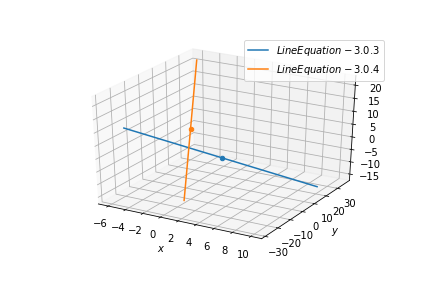
\includegraphics[width=\columnwidth]{./solutions/line_plane/74/codes/figs/Line_interest_1.png}
	\caption{Graph for equations \ref{eq:solutions/line_plane/74/codes7}}
	\label{fig:solutions/line_plane/74/codesline_equation_1}
\end{figure}


	\item 
	\begin{align}\label{eq:solutions/line_plane/74/codes12}
		\frac{x}{2} = \frac{y}{2} &= \frac{z}{1}, 
	\end{align}
	\begin{align}\label{eq:solutions/line_plane/74/codes13}
		\frac{x-5}{4} = \frac{y-2}{1} &= \frac{z-3}{8} 
	\end{align}



The above symmetric equations \ref{eq:solutions/line_plane/74/codes12}, \ref{eq:solutions/line_plane/74/codes13} can be represented in the vector form as 
\begin{align}\label{eq:solutions/line_plane/74/codes14}
	\quad \vec{r_1} &= \myvec{0\\0\\0} + \lambda_1\myvec{2\\2\\1}
	\\
	\quad \vec{r_2} &= \myvec{5\\2\\3} + \lambda_2\myvec{4\\1\\8}
\end{align}

As we have to find the angle between the vectors, we will only be taking the direction vectors into consideration. The direction vectors are $\vec{u}$ = $\myvec{2\\2\\1}$ and $\vec{v}$ = $\myvec{4\\1\\8}$. We can find the corresponding magnitude values

\begin{align}\label{eq:solutions/line_plane/74/codes16}
	\norm{\vec{u}} =\sqrt{2^{2}+2^{2}+1^{2}} =\sqrt{9}
\end{align}
\begin{align}\label{eq:solutions/line_plane/74/codes17}
	\norm{\vec{v}} =\sqrt{4^{2}+1^{2}+8^{2}} =\sqrt{81}
\end{align}

Using \ref{eq:solutions/line_plane/74/codes4}, \ref{eq:solutions/line_plane/74/codes16}, \ref{eq:solutions/line_plane/74/codes17} we get
\begin{align}
	\theta = \cos ^{-1}\frac{\myvec{2\\2\\1}^{T}\myvec{4\\1\\8}}{(\sqrt{9})(\sqrt{81})} 
	\\
	\theta = \cos ^{-1}\frac{18}{27.00}
	\\
	\theta = \cos ^{-1} (0.667)
	\\
	\theta = 48.189\degree
\end{align}

Therefore, the angle between the two lines is $48.189\degree$. See Fig. \ref{fig:solutions/line_plane/74/codesline_equation_2}


\begin{figure}
	\centering
	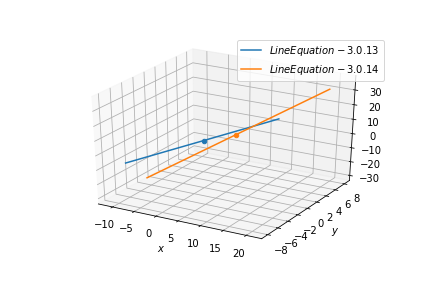
\includegraphics[width=\columnwidth]{./solutions/line_plane/74/codes/figs/Line_interest_2.png}
	\caption{Graph for equations \ref{eq:solutions/line_plane/74/codes14}}
	\label{fig:solutions/line_plane/74/codesline_equation_2}
\end{figure}
\end{enumerate}

    

\item Find $p(0)$, $p(1)$ and $p(2)$ for each of the following polynomials: 
\begin{enumerate}
\item $p(y) = y^2$. 
\item $p(x) = (x – 1) (x + 1)$.
\end{enumerate}
\solution 
From theory, we understand that using dot product we can find the angle between the lines 
\begin{enumerate}
	\item 
	\begin{align}\label{eq:solutions/line_plane/74/codes:5}
		\frac{x-2}{2} = \frac{y-1}{5} &= \frac{z+3}{-3}, 
	\end{align}
	\begin{align}\label{eq:solutions/line_plane/74/codes:6}
		\frac{x+2}{-1} = \frac{y-4}{8} &= \frac{z-5}{4} 
	\end{align}


The above symmetric equations \ref{eq:solutions/line_plane/74/codes:5}, \ref{eq:solutions/line_plane/74/codes:6} can be represented in the vector form as 
\begin{align}\label{eq:solutions/line_plane/74/codes7}
	\quad \vec{r_1} &= \myvec{2\\1\\-3} + \lambda_1\myvec{2\\5\\-3}
	\\
	\quad \vec{r_2} &= \myvec{-2\\4\\5} + \lambda_2\myvec{-1\\8\\4}
\end{align}

As we have to find the angle between the vectors, we will only be taking the direction vectors into consideration. The direction vectors are $\vec{u}$ = $\myvec{2\\5\\-3}$ and $\vec{v}$ = $\myvec{-1\\8\\4}$. We can find the corresponding magnitude values

\begin{align}\label{eq:solutions/line_plane/74/codes9}
	\norm{\vec{u}} =\sqrt{2^{2}+5^{2}+(-3)^{2}} =\sqrt{38}
\end{align}
\begin{align}\label{eq:solutions/line_plane/74/codes10}
	\norm{\vec{v}} =\sqrt{(-1)^{2}+8^{2}+4^{2}} =\sqrt{81}
\end{align}

Using \ref{eq:solutions/line_plane/74/codes4}, \ref{eq:solutions/line_plane/74/codes9}, \ref{eq:solutions/line_plane/74/codes10} we get
\begin{align}
	\theta = \cos ^{-1}\frac{\myvec{2\\5\\-3}^{T}\myvec{-1\\8\\4}}{(\sqrt{38})(\sqrt{81})} 
	\\
	\theta = \cos ^{-1}\frac{26}{55.4797}
	\\
	\theta = \cos ^{-1} (0.4686)
	\\
	\theta = 62.053\degree
\end{align}

Therefore, the angle between the two lines is $62.053\degree$.See Fig. \ref{fig:solutions/line_plane/74/codesline_equation_1}

\begin{figure}
	\centering
	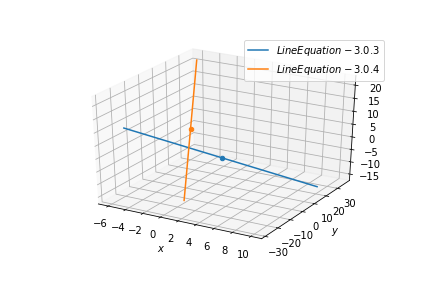
\includegraphics[width=\columnwidth]{./solutions/line_plane/74/codes/figs/Line_interest_1.png}
	\caption{Graph for equations \ref{eq:solutions/line_plane/74/codes7}}
	\label{fig:solutions/line_plane/74/codesline_equation_1}
\end{figure}


	\item 
	\begin{align}\label{eq:solutions/line_plane/74/codes12}
		\frac{x}{2} = \frac{y}{2} &= \frac{z}{1}, 
	\end{align}
	\begin{align}\label{eq:solutions/line_plane/74/codes13}
		\frac{x-5}{4} = \frac{y-2}{1} &= \frac{z-3}{8} 
	\end{align}



The above symmetric equations \ref{eq:solutions/line_plane/74/codes12}, \ref{eq:solutions/line_plane/74/codes13} can be represented in the vector form as 
\begin{align}\label{eq:solutions/line_plane/74/codes14}
	\quad \vec{r_1} &= \myvec{0\\0\\0} + \lambda_1\myvec{2\\2\\1}
	\\
	\quad \vec{r_2} &= \myvec{5\\2\\3} + \lambda_2\myvec{4\\1\\8}
\end{align}

As we have to find the angle between the vectors, we will only be taking the direction vectors into consideration. The direction vectors are $\vec{u}$ = $\myvec{2\\2\\1}$ and $\vec{v}$ = $\myvec{4\\1\\8}$. We can find the corresponding magnitude values

\begin{align}\label{eq:solutions/line_plane/74/codes16}
	\norm{\vec{u}} =\sqrt{2^{2}+2^{2}+1^{2}} =\sqrt{9}
\end{align}
\begin{align}\label{eq:solutions/line_plane/74/codes17}
	\norm{\vec{v}} =\sqrt{4^{2}+1^{2}+8^{2}} =\sqrt{81}
\end{align}

Using \ref{eq:solutions/line_plane/74/codes4}, \ref{eq:solutions/line_plane/74/codes16}, \ref{eq:solutions/line_plane/74/codes17} we get
\begin{align}
	\theta = \cos ^{-1}\frac{\myvec{2\\2\\1}^{T}\myvec{4\\1\\8}}{(\sqrt{9})(\sqrt{81})} 
	\\
	\theta = \cos ^{-1}\frac{18}{27.00}
	\\
	\theta = \cos ^{-1} (0.667)
	\\
	\theta = 48.189\degree
\end{align}

Therefore, the angle between the two lines is $48.189\degree$. See Fig. \ref{fig:solutions/line_plane/74/codesline_equation_2}


\begin{figure}
	\centering
	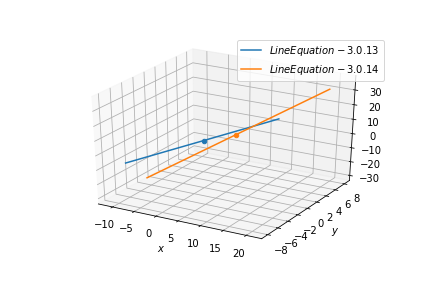
\includegraphics[width=\columnwidth]{./solutions/line_plane/74/codes/figs/Line_interest_2.png}
	\caption{Graph for equations \ref{eq:solutions/line_plane/74/codes14}}
	\label{fig:solutions/line_plane/74/codesline_equation_2}
\end{figure}
\end{enumerate}

    

\item Find the roots of the quadratic equation $6x^2– x – 2 = 0.$
\\
\solution 
	
The vector form of 
\begin{align}
y = 6x^2-x-2 
\end{align}
is
\begin{align}
	\vec{x}^T\myvec{6&0\\0&0}\vec{x}  + \myvec{-1&-1}\vec{x} -2 = 0
	\end{align}
	Thus, 
	\begin{align}
	y = 0 \quad \implies 6x^2-x-2 &= 0
	\\
	\brak{x+\frac{1}{2}}\brak{x-\frac{2}{3}} &= 0
	\\
	x = \frac{-1}{2},\frac{2}{3}&
	\end{align}
	The following python code computes roots of the quadratic equation represented in Fig. \ref{fig:5.1.5_qnineteen}.
	\begin{lstlisting}
	./solutions/5/codes/conics/q19.py
	\end{lstlisting}
	\begin{figure}[!ht]
	\centering
	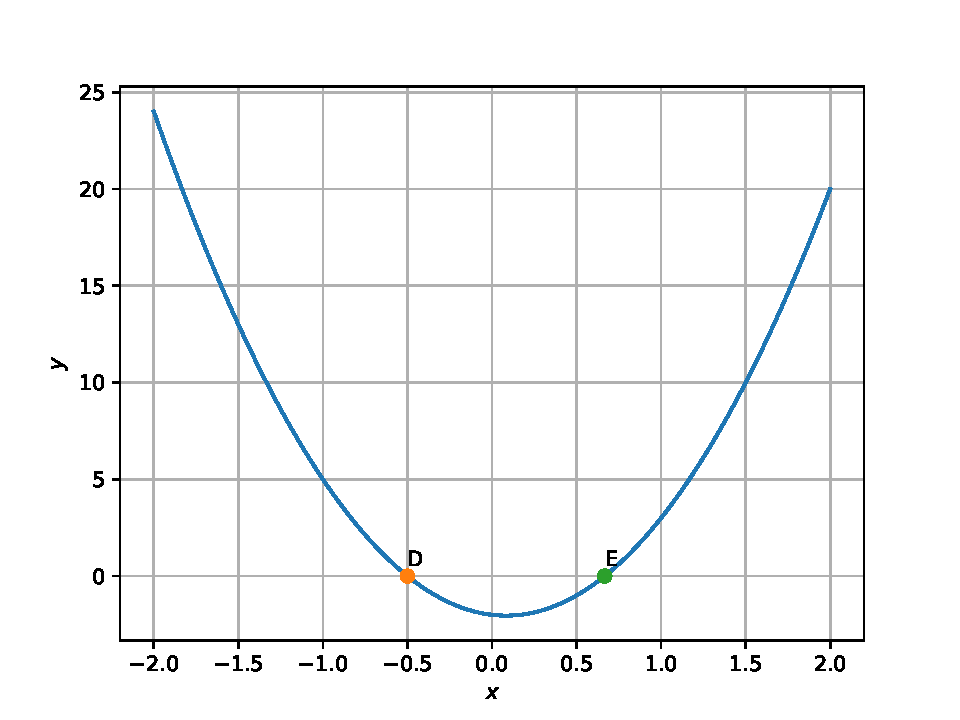
\includegraphics[width=\columnwidth]{./solutions/5/figs/conics/q19.eps}
	\caption{}
	\label{fig:5.1.5_qnineteen}	
	\end{figure}
	
	

\item Find the roots of the quadratic equation $3x^2 -2 \sqrt{6}x+ 2 = 0$.
\\
\solution 
From theory, we understand that using dot product we can find the angle between the lines 
\begin{enumerate}
	\item 
	\begin{align}\label{eq:solutions/line_plane/74/codes:5}
		\frac{x-2}{2} = \frac{y-1}{5} &= \frac{z+3}{-3}, 
	\end{align}
	\begin{align}\label{eq:solutions/line_plane/74/codes:6}
		\frac{x+2}{-1} = \frac{y-4}{8} &= \frac{z-5}{4} 
	\end{align}


The above symmetric equations \ref{eq:solutions/line_plane/74/codes:5}, \ref{eq:solutions/line_plane/74/codes:6} can be represented in the vector form as 
\begin{align}\label{eq:solutions/line_plane/74/codes7}
	\quad \vec{r_1} &= \myvec{2\\1\\-3} + \lambda_1\myvec{2\\5\\-3}
	\\
	\quad \vec{r_2} &= \myvec{-2\\4\\5} + \lambda_2\myvec{-1\\8\\4}
\end{align}

As we have to find the angle between the vectors, we will only be taking the direction vectors into consideration. The direction vectors are $\vec{u}$ = $\myvec{2\\5\\-3}$ and $\vec{v}$ = $\myvec{-1\\8\\4}$. We can find the corresponding magnitude values

\begin{align}\label{eq:solutions/line_plane/74/codes9}
	\norm{\vec{u}} =\sqrt{2^{2}+5^{2}+(-3)^{2}} =\sqrt{38}
\end{align}
\begin{align}\label{eq:solutions/line_plane/74/codes10}
	\norm{\vec{v}} =\sqrt{(-1)^{2}+8^{2}+4^{2}} =\sqrt{81}
\end{align}

Using \ref{eq:solutions/line_plane/74/codes4}, \ref{eq:solutions/line_plane/74/codes9}, \ref{eq:solutions/line_plane/74/codes10} we get
\begin{align}
	\theta = \cos ^{-1}\frac{\myvec{2\\5\\-3}^{T}\myvec{-1\\8\\4}}{(\sqrt{38})(\sqrt{81})} 
	\\
	\theta = \cos ^{-1}\frac{26}{55.4797}
	\\
	\theta = \cos ^{-1} (0.4686)
	\\
	\theta = 62.053\degree
\end{align}

Therefore, the angle between the two lines is $62.053\degree$.See Fig. \ref{fig:solutions/line_plane/74/codesline_equation_1}

\begin{figure}
	\centering
	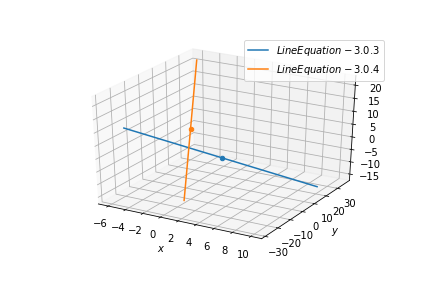
\includegraphics[width=\columnwidth]{./solutions/line_plane/74/codes/figs/Line_interest_1.png}
	\caption{Graph for equations \ref{eq:solutions/line_plane/74/codes7}}
	\label{fig:solutions/line_plane/74/codesline_equation_1}
\end{figure}


	\item 
	\begin{align}\label{eq:solutions/line_plane/74/codes12}
		\frac{x}{2} = \frac{y}{2} &= \frac{z}{1}, 
	\end{align}
	\begin{align}\label{eq:solutions/line_plane/74/codes13}
		\frac{x-5}{4} = \frac{y-2}{1} &= \frac{z-3}{8} 
	\end{align}



The above symmetric equations \ref{eq:solutions/line_plane/74/codes12}, \ref{eq:solutions/line_plane/74/codes13} can be represented in the vector form as 
\begin{align}\label{eq:solutions/line_plane/74/codes14}
	\quad \vec{r_1} &= \myvec{0\\0\\0} + \lambda_1\myvec{2\\2\\1}
	\\
	\quad \vec{r_2} &= \myvec{5\\2\\3} + \lambda_2\myvec{4\\1\\8}
\end{align}

As we have to find the angle between the vectors, we will only be taking the direction vectors into consideration. The direction vectors are $\vec{u}$ = $\myvec{2\\2\\1}$ and $\vec{v}$ = $\myvec{4\\1\\8}$. We can find the corresponding magnitude values

\begin{align}\label{eq:solutions/line_plane/74/codes16}
	\norm{\vec{u}} =\sqrt{2^{2}+2^{2}+1^{2}} =\sqrt{9}
\end{align}
\begin{align}\label{eq:solutions/line_plane/74/codes17}
	\norm{\vec{v}} =\sqrt{4^{2}+1^{2}+8^{2}} =\sqrt{81}
\end{align}

Using \ref{eq:solutions/line_plane/74/codes4}, \ref{eq:solutions/line_plane/74/codes16}, \ref{eq:solutions/line_plane/74/codes17} we get
\begin{align}
	\theta = \cos ^{-1}\frac{\myvec{2\\2\\1}^{T}\myvec{4\\1\\8}}{(\sqrt{9})(\sqrt{81})} 
	\\
	\theta = \cos ^{-1}\frac{18}{27.00}
	\\
	\theta = \cos ^{-1} (0.667)
	\\
	\theta = 48.189\degree
\end{align}

Therefore, the angle between the two lines is $48.189\degree$. See Fig. \ref{fig:solutions/line_plane/74/codesline_equation_2}


\begin{figure}
	\centering
	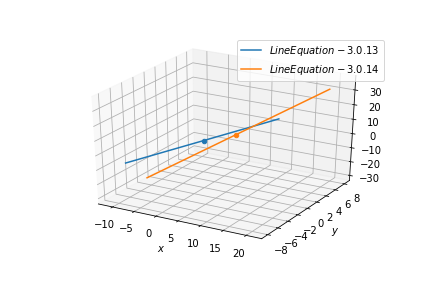
\includegraphics[width=\columnwidth]{./solutions/line_plane/74/codes/figs/Line_interest_2.png}
	\caption{Graph for equations \ref{eq:solutions/line_plane/74/codes14}}
	\label{fig:solutions/line_plane/74/codesline_equation_2}
\end{figure}
\end{enumerate}

    

\item Verify whether the following are zeroes of the polynomial, indicated against them. 
%\item p(x) = 3x + 1, x =
\begin{enumerate}

\item $ p(x) = x^2-1, x = 1, -1$
\item $ p(x) = \brak{x+1} \brak{x-2}, x = -1,2$
\item $ p(x) = x^2, x = 0$.
\item $ p(x) = 3x^2-1, x = -\frac{1}{\sqrt{3}}, \frac{2}{\sqrt{3}}$.
\end{enumerate}
\solution 
From theory, we understand that using dot product we can find the angle between the lines 
\begin{enumerate}
	\item 
	\begin{align}\label{eq:solutions/line_plane/74/codes:5}
		\frac{x-2}{2} = \frac{y-1}{5} &= \frac{z+3}{-3}, 
	\end{align}
	\begin{align}\label{eq:solutions/line_plane/74/codes:6}
		\frac{x+2}{-1} = \frac{y-4}{8} &= \frac{z-5}{4} 
	\end{align}


The above symmetric equations \ref{eq:solutions/line_plane/74/codes:5}, \ref{eq:solutions/line_plane/74/codes:6} can be represented in the vector form as 
\begin{align}\label{eq:solutions/line_plane/74/codes7}
	\quad \vec{r_1} &= \myvec{2\\1\\-3} + \lambda_1\myvec{2\\5\\-3}
	\\
	\quad \vec{r_2} &= \myvec{-2\\4\\5} + \lambda_2\myvec{-1\\8\\4}
\end{align}

As we have to find the angle between the vectors, we will only be taking the direction vectors into consideration. The direction vectors are $\vec{u}$ = $\myvec{2\\5\\-3}$ and $\vec{v}$ = $\myvec{-1\\8\\4}$. We can find the corresponding magnitude values

\begin{align}\label{eq:solutions/line_plane/74/codes9}
	\norm{\vec{u}} =\sqrt{2^{2}+5^{2}+(-3)^{2}} =\sqrt{38}
\end{align}
\begin{align}\label{eq:solutions/line_plane/74/codes10}
	\norm{\vec{v}} =\sqrt{(-1)^{2}+8^{2}+4^{2}} =\sqrt{81}
\end{align}

Using \ref{eq:solutions/line_plane/74/codes4}, \ref{eq:solutions/line_plane/74/codes9}, \ref{eq:solutions/line_plane/74/codes10} we get
\begin{align}
	\theta = \cos ^{-1}\frac{\myvec{2\\5\\-3}^{T}\myvec{-1\\8\\4}}{(\sqrt{38})(\sqrt{81})} 
	\\
	\theta = \cos ^{-1}\frac{26}{55.4797}
	\\
	\theta = \cos ^{-1} (0.4686)
	\\
	\theta = 62.053\degree
\end{align}

Therefore, the angle between the two lines is $62.053\degree$.See Fig. \ref{fig:solutions/line_plane/74/codesline_equation_1}

\begin{figure}
	\centering
	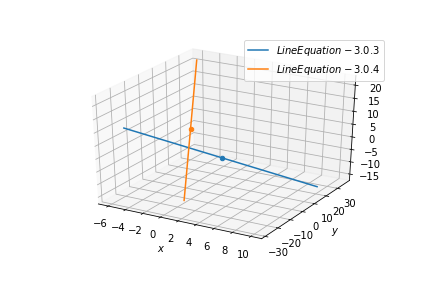
\includegraphics[width=\columnwidth]{./solutions/line_plane/74/codes/figs/Line_interest_1.png}
	\caption{Graph for equations \ref{eq:solutions/line_plane/74/codes7}}
	\label{fig:solutions/line_plane/74/codesline_equation_1}
\end{figure}


	\item 
	\begin{align}\label{eq:solutions/line_plane/74/codes12}
		\frac{x}{2} = \frac{y}{2} &= \frac{z}{1}, 
	\end{align}
	\begin{align}\label{eq:solutions/line_plane/74/codes13}
		\frac{x-5}{4} = \frac{y-2}{1} &= \frac{z-3}{8} 
	\end{align}



The above symmetric equations \ref{eq:solutions/line_plane/74/codes12}, \ref{eq:solutions/line_plane/74/codes13} can be represented in the vector form as 
\begin{align}\label{eq:solutions/line_plane/74/codes14}
	\quad \vec{r_1} &= \myvec{0\\0\\0} + \lambda_1\myvec{2\\2\\1}
	\\
	\quad \vec{r_2} &= \myvec{5\\2\\3} + \lambda_2\myvec{4\\1\\8}
\end{align}

As we have to find the angle between the vectors, we will only be taking the direction vectors into consideration. The direction vectors are $\vec{u}$ = $\myvec{2\\2\\1}$ and $\vec{v}$ = $\myvec{4\\1\\8}$. We can find the corresponding magnitude values

\begin{align}\label{eq:solutions/line_plane/74/codes16}
	\norm{\vec{u}} =\sqrt{2^{2}+2^{2}+1^{2}} =\sqrt{9}
\end{align}
\begin{align}\label{eq:solutions/line_plane/74/codes17}
	\norm{\vec{v}} =\sqrt{4^{2}+1^{2}+8^{2}} =\sqrt{81}
\end{align}

Using \ref{eq:solutions/line_plane/74/codes4}, \ref{eq:solutions/line_plane/74/codes16}, \ref{eq:solutions/line_plane/74/codes17} we get
\begin{align}
	\theta = \cos ^{-1}\frac{\myvec{2\\2\\1}^{T}\myvec{4\\1\\8}}{(\sqrt{9})(\sqrt{81})} 
	\\
	\theta = \cos ^{-1}\frac{18}{27.00}
	\\
	\theta = \cos ^{-1} (0.667)
	\\
	\theta = 48.189\degree
\end{align}

Therefore, the angle between the two lines is $48.189\degree$. See Fig. \ref{fig:solutions/line_plane/74/codesline_equation_2}


\begin{figure}
	\centering
	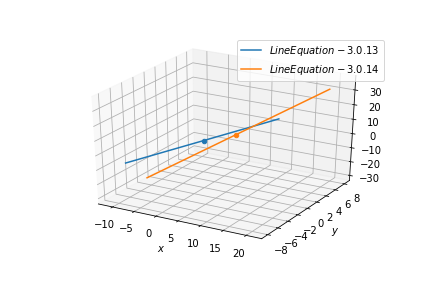
\includegraphics[width=\columnwidth]{./solutions/line_plane/74/codes/figs/Line_interest_2.png}
	\caption{Graph for equations \ref{eq:solutions/line_plane/74/codes14}}
	\label{fig:solutions/line_plane/74/codesline_equation_2}
\end{figure}
\end{enumerate}

    

\item Solve each of the following equations
\begin{enumerate}
\item 	$3x^2-4x+\frac{20}{3} = 0$
\item 	$x^2-2x+\frac{3}{2} = 0$
\item 	$27x^2-10x+1 = 0$
\item 	$21x^2-28x+10 = 0$
\end{enumerate}
%
\solution 
From theory, we understand that using dot product we can find the angle between the lines 
\begin{enumerate}
	\item 
	\begin{align}\label{eq:solutions/line_plane/74/codes:5}
		\frac{x-2}{2} = \frac{y-1}{5} &= \frac{z+3}{-3}, 
	\end{align}
	\begin{align}\label{eq:solutions/line_plane/74/codes:6}
		\frac{x+2}{-1} = \frac{y-4}{8} &= \frac{z-5}{4} 
	\end{align}


The above symmetric equations \ref{eq:solutions/line_plane/74/codes:5}, \ref{eq:solutions/line_plane/74/codes:6} can be represented in the vector form as 
\begin{align}\label{eq:solutions/line_plane/74/codes7}
	\quad \vec{r_1} &= \myvec{2\\1\\-3} + \lambda_1\myvec{2\\5\\-3}
	\\
	\quad \vec{r_2} &= \myvec{-2\\4\\5} + \lambda_2\myvec{-1\\8\\4}
\end{align}

As we have to find the angle between the vectors, we will only be taking the direction vectors into consideration. The direction vectors are $\vec{u}$ = $\myvec{2\\5\\-3}$ and $\vec{v}$ = $\myvec{-1\\8\\4}$. We can find the corresponding magnitude values

\begin{align}\label{eq:solutions/line_plane/74/codes9}
	\norm{\vec{u}} =\sqrt{2^{2}+5^{2}+(-3)^{2}} =\sqrt{38}
\end{align}
\begin{align}\label{eq:solutions/line_plane/74/codes10}
	\norm{\vec{v}} =\sqrt{(-1)^{2}+8^{2}+4^{2}} =\sqrt{81}
\end{align}

Using \ref{eq:solutions/line_plane/74/codes4}, \ref{eq:solutions/line_plane/74/codes9}, \ref{eq:solutions/line_plane/74/codes10} we get
\begin{align}
	\theta = \cos ^{-1}\frac{\myvec{2\\5\\-3}^{T}\myvec{-1\\8\\4}}{(\sqrt{38})(\sqrt{81})} 
	\\
	\theta = \cos ^{-1}\frac{26}{55.4797}
	\\
	\theta = \cos ^{-1} (0.4686)
	\\
	\theta = 62.053\degree
\end{align}

Therefore, the angle between the two lines is $62.053\degree$.See Fig. \ref{fig:solutions/line_plane/74/codesline_equation_1}

\begin{figure}
	\centering
	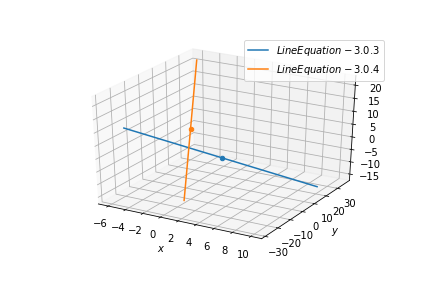
\includegraphics[width=\columnwidth]{./solutions/line_plane/74/codes/figs/Line_interest_1.png}
	\caption{Graph for equations \ref{eq:solutions/line_plane/74/codes7}}
	\label{fig:solutions/line_plane/74/codesline_equation_1}
\end{figure}


	\item 
	\begin{align}\label{eq:solutions/line_plane/74/codes12}
		\frac{x}{2} = \frac{y}{2} &= \frac{z}{1}, 
	\end{align}
	\begin{align}\label{eq:solutions/line_plane/74/codes13}
		\frac{x-5}{4} = \frac{y-2}{1} &= \frac{z-3}{8} 
	\end{align}



The above symmetric equations \ref{eq:solutions/line_plane/74/codes12}, \ref{eq:solutions/line_plane/74/codes13} can be represented in the vector form as 
\begin{align}\label{eq:solutions/line_plane/74/codes14}
	\quad \vec{r_1} &= \myvec{0\\0\\0} + \lambda_1\myvec{2\\2\\1}
	\\
	\quad \vec{r_2} &= \myvec{5\\2\\3} + \lambda_2\myvec{4\\1\\8}
\end{align}

As we have to find the angle between the vectors, we will only be taking the direction vectors into consideration. The direction vectors are $\vec{u}$ = $\myvec{2\\2\\1}$ and $\vec{v}$ = $\myvec{4\\1\\8}$. We can find the corresponding magnitude values

\begin{align}\label{eq:solutions/line_plane/74/codes16}
	\norm{\vec{u}} =\sqrt{2^{2}+2^{2}+1^{2}} =\sqrt{9}
\end{align}
\begin{align}\label{eq:solutions/line_plane/74/codes17}
	\norm{\vec{v}} =\sqrt{4^{2}+1^{2}+8^{2}} =\sqrt{81}
\end{align}

Using \ref{eq:solutions/line_plane/74/codes4}, \ref{eq:solutions/line_plane/74/codes16}, \ref{eq:solutions/line_plane/74/codes17} we get
\begin{align}
	\theta = \cos ^{-1}\frac{\myvec{2\\2\\1}^{T}\myvec{4\\1\\8}}{(\sqrt{9})(\sqrt{81})} 
	\\
	\theta = \cos ^{-1}\frac{18}{27.00}
	\\
	\theta = \cos ^{-1} (0.667)
	\\
	\theta = 48.189\degree
\end{align}

Therefore, the angle between the two lines is $48.189\degree$. See Fig. \ref{fig:solutions/line_plane/74/codesline_equation_2}


\begin{figure}
	\centering
	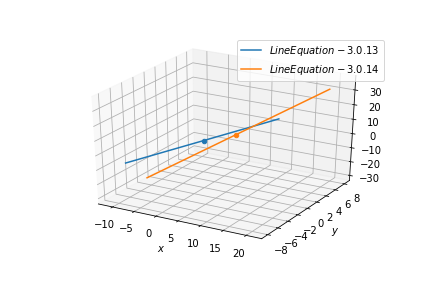
\includegraphics[width=\columnwidth]{./solutions/line_plane/74/codes/figs/Line_interest_2.png}
	\caption{Graph for equations \ref{eq:solutions/line_plane/74/codes14}}
	\label{fig:solutions/line_plane/74/codesline_equation_2}
\end{figure}
\end{enumerate}

    


%
\item  Factorise 
\begin{enumerate}
\item $12x^2 – 7x + 1 $
\item $6x^2+ 5x – 6$
\item $2x^2+ 7x + 3 $
\item $3x^2– x – 4$
\end{enumerate}
\solution 
From theory, we understand that using dot product we can find the angle between the lines 
\begin{enumerate}
	\item 
	\begin{align}\label{eq:solutions/line_plane/74/codes:5}
		\frac{x-2}{2} = \frac{y-1}{5} &= \frac{z+3}{-3}, 
	\end{align}
	\begin{align}\label{eq:solutions/line_plane/74/codes:6}
		\frac{x+2}{-1} = \frac{y-4}{8} &= \frac{z-5}{4} 
	\end{align}


The above symmetric equations \ref{eq:solutions/line_plane/74/codes:5}, \ref{eq:solutions/line_plane/74/codes:6} can be represented in the vector form as 
\begin{align}\label{eq:solutions/line_plane/74/codes7}
	\quad \vec{r_1} &= \myvec{2\\1\\-3} + \lambda_1\myvec{2\\5\\-3}
	\\
	\quad \vec{r_2} &= \myvec{-2\\4\\5} + \lambda_2\myvec{-1\\8\\4}
\end{align}

As we have to find the angle between the vectors, we will only be taking the direction vectors into consideration. The direction vectors are $\vec{u}$ = $\myvec{2\\5\\-3}$ and $\vec{v}$ = $\myvec{-1\\8\\4}$. We can find the corresponding magnitude values

\begin{align}\label{eq:solutions/line_plane/74/codes9}
	\norm{\vec{u}} =\sqrt{2^{2}+5^{2}+(-3)^{2}} =\sqrt{38}
\end{align}
\begin{align}\label{eq:solutions/line_plane/74/codes10}
	\norm{\vec{v}} =\sqrt{(-1)^{2}+8^{2}+4^{2}} =\sqrt{81}
\end{align}

Using \ref{eq:solutions/line_plane/74/codes4}, \ref{eq:solutions/line_plane/74/codes9}, \ref{eq:solutions/line_plane/74/codes10} we get
\begin{align}
	\theta = \cos ^{-1}\frac{\myvec{2\\5\\-3}^{T}\myvec{-1\\8\\4}}{(\sqrt{38})(\sqrt{81})} 
	\\
	\theta = \cos ^{-1}\frac{26}{55.4797}
	\\
	\theta = \cos ^{-1} (0.4686)
	\\
	\theta = 62.053\degree
\end{align}

Therefore, the angle between the two lines is $62.053\degree$.See Fig. \ref{fig:solutions/line_plane/74/codesline_equation_1}

\begin{figure}
	\centering
	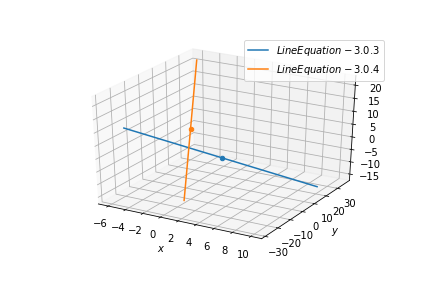
\includegraphics[width=\columnwidth]{./solutions/line_plane/74/codes/figs/Line_interest_1.png}
	\caption{Graph for equations \ref{eq:solutions/line_plane/74/codes7}}
	\label{fig:solutions/line_plane/74/codesline_equation_1}
\end{figure}


	\item 
	\begin{align}\label{eq:solutions/line_plane/74/codes12}
		\frac{x}{2} = \frac{y}{2} &= \frac{z}{1}, 
	\end{align}
	\begin{align}\label{eq:solutions/line_plane/74/codes13}
		\frac{x-5}{4} = \frac{y-2}{1} &= \frac{z-3}{8} 
	\end{align}



The above symmetric equations \ref{eq:solutions/line_plane/74/codes12}, \ref{eq:solutions/line_plane/74/codes13} can be represented in the vector form as 
\begin{align}\label{eq:solutions/line_plane/74/codes14}
	\quad \vec{r_1} &= \myvec{0\\0\\0} + \lambda_1\myvec{2\\2\\1}
	\\
	\quad \vec{r_2} &= \myvec{5\\2\\3} + \lambda_2\myvec{4\\1\\8}
\end{align}

As we have to find the angle between the vectors, we will only be taking the direction vectors into consideration. The direction vectors are $\vec{u}$ = $\myvec{2\\2\\1}$ and $\vec{v}$ = $\myvec{4\\1\\8}$. We can find the corresponding magnitude values

\begin{align}\label{eq:solutions/line_plane/74/codes16}
	\norm{\vec{u}} =\sqrt{2^{2}+2^{2}+1^{2}} =\sqrt{9}
\end{align}
\begin{align}\label{eq:solutions/line_plane/74/codes17}
	\norm{\vec{v}} =\sqrt{4^{2}+1^{2}+8^{2}} =\sqrt{81}
\end{align}

Using \ref{eq:solutions/line_plane/74/codes4}, \ref{eq:solutions/line_plane/74/codes16}, \ref{eq:solutions/line_plane/74/codes17} we get
\begin{align}
	\theta = \cos ^{-1}\frac{\myvec{2\\2\\1}^{T}\myvec{4\\1\\8}}{(\sqrt{9})(\sqrt{81})} 
	\\
	\theta = \cos ^{-1}\frac{18}{27.00}
	\\
	\theta = \cos ^{-1} (0.667)
	\\
	\theta = 48.189\degree
\end{align}

Therefore, the angle between the two lines is $48.189\degree$. See Fig. \ref{fig:solutions/line_plane/74/codesline_equation_2}


\begin{figure}
	\centering
	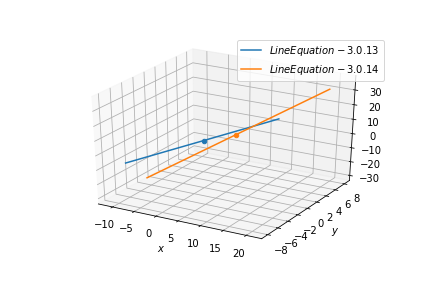
\includegraphics[width=\columnwidth]{./solutions/line_plane/74/codes/figs/Line_interest_2.png}
	\caption{Graph for equations \ref{eq:solutions/line_plane/74/codes14}}
	\label{fig:solutions/line_plane/74/codesline_equation_2}
\end{figure}
\end{enumerate}

    

\item Find the zeroes of the following quadratic polynomials and verify the relationship between the zeroes and the coefficients.
\begin{enumerate}
\item $x^2 – 2x – 8$
\item  $4u^2 + 8u$
\item $4s^2 – 4s + 1$
\item $t^2 – 15$
\item $6x^2– 3 – 7x $
\item $3x^2 – x – 4$
\end{enumerate}
\solution 
From theory, we understand that using dot product we can find the angle between the lines 
\begin{enumerate}
	\item 
	\begin{align}\label{eq:solutions/line_plane/74/codes:5}
		\frac{x-2}{2} = \frac{y-1}{5} &= \frac{z+3}{-3}, 
	\end{align}
	\begin{align}\label{eq:solutions/line_plane/74/codes:6}
		\frac{x+2}{-1} = \frac{y-4}{8} &= \frac{z-5}{4} 
	\end{align}


The above symmetric equations \ref{eq:solutions/line_plane/74/codes:5}, \ref{eq:solutions/line_plane/74/codes:6} can be represented in the vector form as 
\begin{align}\label{eq:solutions/line_plane/74/codes7}
	\quad \vec{r_1} &= \myvec{2\\1\\-3} + \lambda_1\myvec{2\\5\\-3}
	\\
	\quad \vec{r_2} &= \myvec{-2\\4\\5} + \lambda_2\myvec{-1\\8\\4}
\end{align}

As we have to find the angle between the vectors, we will only be taking the direction vectors into consideration. The direction vectors are $\vec{u}$ = $\myvec{2\\5\\-3}$ and $\vec{v}$ = $\myvec{-1\\8\\4}$. We can find the corresponding magnitude values

\begin{align}\label{eq:solutions/line_plane/74/codes9}
	\norm{\vec{u}} =\sqrt{2^{2}+5^{2}+(-3)^{2}} =\sqrt{38}
\end{align}
\begin{align}\label{eq:solutions/line_plane/74/codes10}
	\norm{\vec{v}} =\sqrt{(-1)^{2}+8^{2}+4^{2}} =\sqrt{81}
\end{align}

Using \ref{eq:solutions/line_plane/74/codes4}, \ref{eq:solutions/line_plane/74/codes9}, \ref{eq:solutions/line_plane/74/codes10} we get
\begin{align}
	\theta = \cos ^{-1}\frac{\myvec{2\\5\\-3}^{T}\myvec{-1\\8\\4}}{(\sqrt{38})(\sqrt{81})} 
	\\
	\theta = \cos ^{-1}\frac{26}{55.4797}
	\\
	\theta = \cos ^{-1} (0.4686)
	\\
	\theta = 62.053\degree
\end{align}

Therefore, the angle between the two lines is $62.053\degree$.See Fig. \ref{fig:solutions/line_plane/74/codesline_equation_1}

\begin{figure}
	\centering
	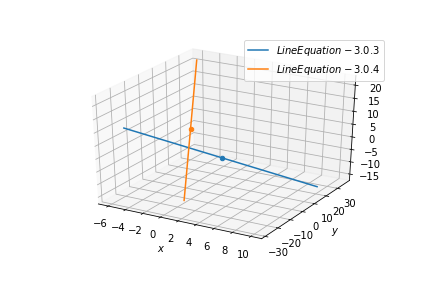
\includegraphics[width=\columnwidth]{./solutions/line_plane/74/codes/figs/Line_interest_1.png}
	\caption{Graph for equations \ref{eq:solutions/line_plane/74/codes7}}
	\label{fig:solutions/line_plane/74/codesline_equation_1}
\end{figure}


	\item 
	\begin{align}\label{eq:solutions/line_plane/74/codes12}
		\frac{x}{2} = \frac{y}{2} &= \frac{z}{1}, 
	\end{align}
	\begin{align}\label{eq:solutions/line_plane/74/codes13}
		\frac{x-5}{4} = \frac{y-2}{1} &= \frac{z-3}{8} 
	\end{align}



The above symmetric equations \ref{eq:solutions/line_plane/74/codes12}, \ref{eq:solutions/line_plane/74/codes13} can be represented in the vector form as 
\begin{align}\label{eq:solutions/line_plane/74/codes14}
	\quad \vec{r_1} &= \myvec{0\\0\\0} + \lambda_1\myvec{2\\2\\1}
	\\
	\quad \vec{r_2} &= \myvec{5\\2\\3} + \lambda_2\myvec{4\\1\\8}
\end{align}

As we have to find the angle between the vectors, we will only be taking the direction vectors into consideration. The direction vectors are $\vec{u}$ = $\myvec{2\\2\\1}$ and $\vec{v}$ = $\myvec{4\\1\\8}$. We can find the corresponding magnitude values

\begin{align}\label{eq:solutions/line_plane/74/codes16}
	\norm{\vec{u}} =\sqrt{2^{2}+2^{2}+1^{2}} =\sqrt{9}
\end{align}
\begin{align}\label{eq:solutions/line_plane/74/codes17}
	\norm{\vec{v}} =\sqrt{4^{2}+1^{2}+8^{2}} =\sqrt{81}
\end{align}

Using \ref{eq:solutions/line_plane/74/codes4}, \ref{eq:solutions/line_plane/74/codes16}, \ref{eq:solutions/line_plane/74/codes17} we get
\begin{align}
	\theta = \cos ^{-1}\frac{\myvec{2\\2\\1}^{T}\myvec{4\\1\\8}}{(\sqrt{9})(\sqrt{81})} 
	\\
	\theta = \cos ^{-1}\frac{18}{27.00}
	\\
	\theta = \cos ^{-1} (0.667)
	\\
	\theta = 48.189\degree
\end{align}

Therefore, the angle between the two lines is $48.189\degree$. See Fig. \ref{fig:solutions/line_plane/74/codesline_equation_2}


\begin{figure}
	\centering
	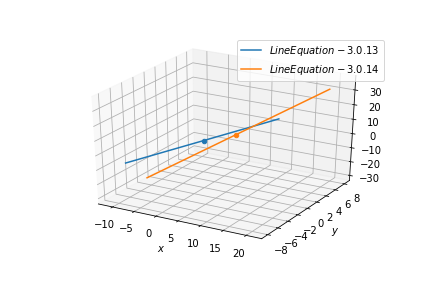
\includegraphics[width=\columnwidth]{./solutions/line_plane/74/codes/figs/Line_interest_2.png}
	\caption{Graph for equations \ref{eq:solutions/line_plane/74/codes14}}
	\label{fig:solutions/line_plane/74/codesline_equation_2}
\end{figure}
\end{enumerate}

    

\item  Find a quadratic polynomial each with the given numbers as the sum and product of its zeroes respectively.
\begin{enumerate}
\item-1 , $\frac{1}{ 4}$
\item 1, 1
\item $0, \sqrt{5}$ 
\item 4, 1
 \item $\frac{1}{4}, \frac{1}{4}$
\item  $\sqrt{2}, \frac{1}{ 3}$
\end{enumerate}
\solution 
The following python code computes roots of the quadratic equation obtained:
	\begin{lstlisting}
	./solutions/5/codes/conics/q20a.py
	./solutions/5/codes/conics/q20b.py
	./solutions/5/codes/conics/q20c.py
	./solutions/5/codes/conics/q20d.py
	./solutions/5/codes/conics/q20e.py
	./solutions/5/codes/conics/q20f.py
	\end{lstlisting}
	
	\begin{enumerate}
	
		\item -1,$\frac{1}{4}$
	\begin{figure}[!ht]
	\centering
	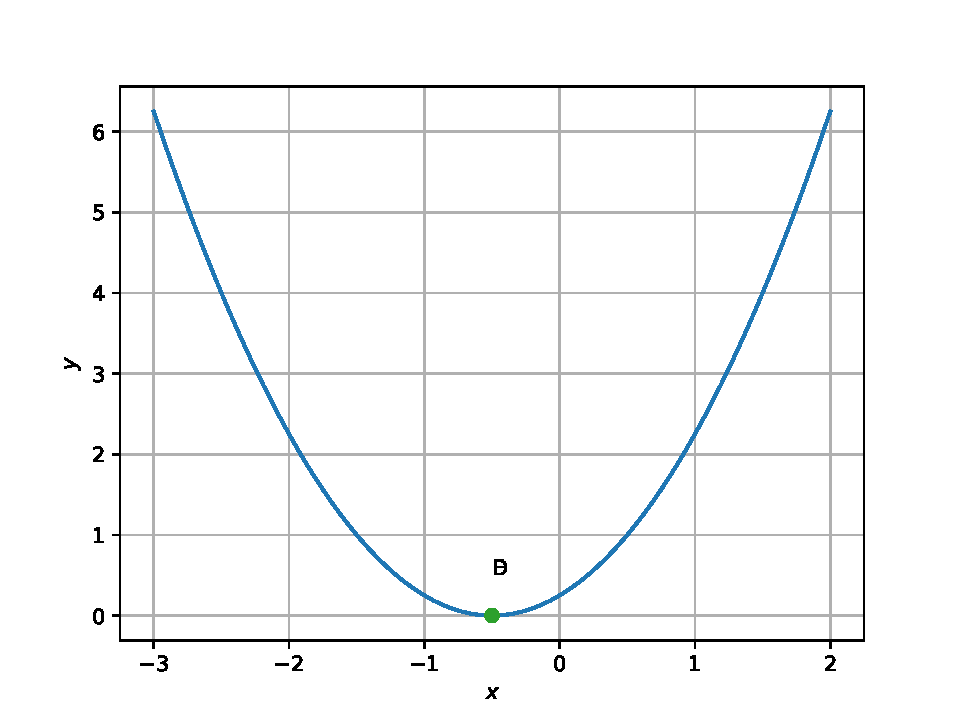
\includegraphics[width=\columnwidth]{./solutions/5/figs/conics/q20a.eps}
	\caption{}
	\label{fig:5.2.5_qtoa}	
	\end{figure}
	
		 For a general polynomial equation of degree 2,
	\begin{multline}
	p\brak{x,y} =
\\
 Ax^2 +Bxy + Cy^2 +Dx + Ey + F = 0\\
	\text{The vector form is}\\
	\vec{x}^T\myvec{A&\frac{B}{2}\\\frac{B}{2}&C}\vec{x}  + \myvec{D&E}\vec{x} + F = 0 \label{eq:5.2.5_qtwenty}
	\end{multline}
Here, sum of zeroes = D = -1\\
Product of zeroes = F =$\frac{1}{4}$\\
Substituing the values in \ref{eq:5.2.5_qtwenty},\\
\begin{multline}
\vec{x}^T\myvec{1&0\\0&0}\vec{x}  + 
\myvec{1&-1}\vec{x} +\frac{1}{4} = 0\\
\end{multline}
\begin{align}
\implies y = x^2 + x + \frac{1}{4}
\end{align}
The roots are -0.5 and -0.5 as represented in Fig. \ref{fig:5.2.5_qtoa}
		
		\item 1,1
	\begin{figure}[!ht]
	\centering
	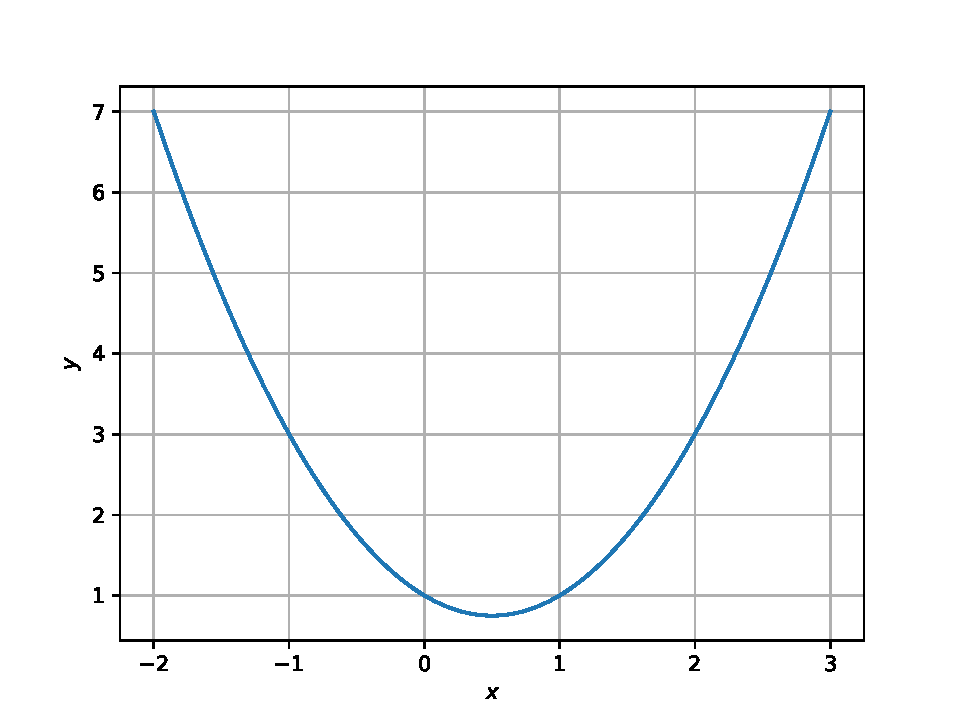
\includegraphics[width=\columnwidth]{./solutions/5/figs/conics/q20b.eps}
	\caption{}
	\label{fig:5.2.5_qtob}	
	\end{figure}
	
		
Here, sum of zeroes = D = 1\\
Product of zeroes = F =1\\
Substituing the values in \ref{eq:5.2.5_qtwenty},\\
\begin{multline}
\vec{x}^T\myvec{1&0\\0&0}\vec{x}  + \myvec{-1&-1}\vec{x} +1 = 0
\end{multline}
\begin{align}
\implies y = x^2 - x + 1 
\end{align}
Since the curve doesn't meet the x-axis, real roots don't exist for this parabola as represented in Fig. \ref{fig:5.2.5_qtob}	
		\item 0,$\sqrt{5}$
			\begin{figure}[!ht]
	\centering
	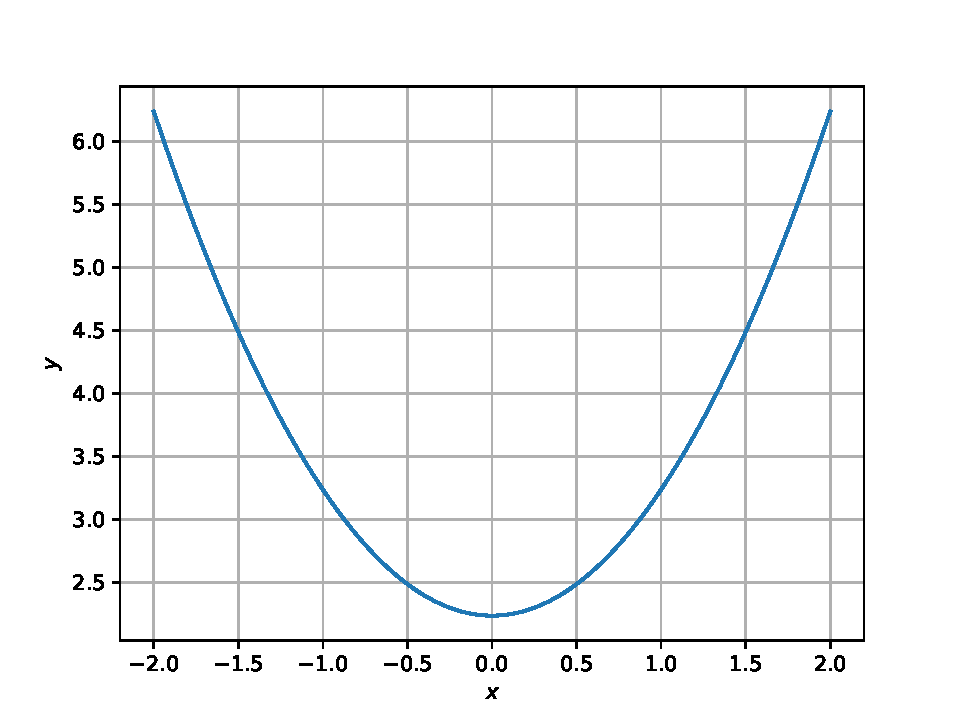
\includegraphics[width=\columnwidth]{./solutions/5/figs/conics/q20c.eps}
	\caption{}
	\label{fig:5.2.5_qtoc}	
	\end{figure}

		
Here, sum of zeroes = D = 0\\
Product of zeroes = F =$\sqrt{5}$\\
Substituing the values in \ref{eq:5.2.5_qtwenty},\\
\begin{multline}
\vec{x}^T\myvec{1&0\\0&0}\vec{x}  + \myvec{0&-1}\vec{x} + \sqrt{5} = 0
\end{multline}
\begin{align}
\implies y = x^2 + \sqrt{5}  
\end{align}
Since the curve doesn't meet the x-axis, real roots don't exist for this parabola as represented in Fig. \ref{fig:5.2.5_qtoc}	
		\item 4,1
	\begin{figure}[!ht]
	\centering
	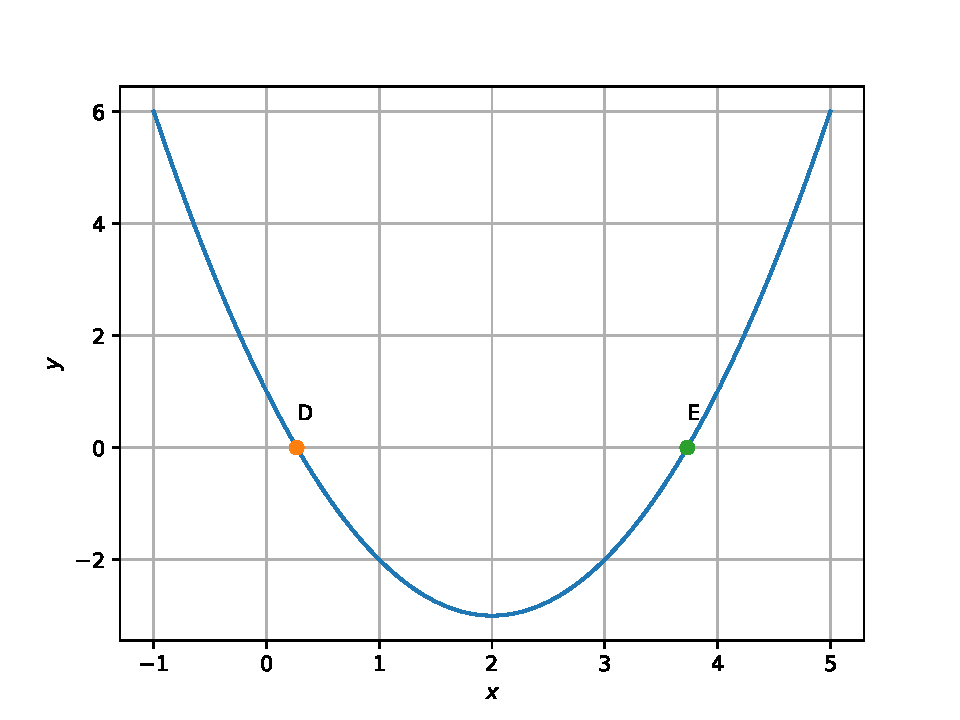
\includegraphics[width=\columnwidth]{./solutions/5/figs/conics/q20d.eps}
	\caption{}
	\label{fig:5.2.5_qtod}	
	\end{figure}
	
		 
Here, sum of zeroes = D = 4\\
Product of zeroes = F = 1\\
Substituing the values in \ref{eq:5.2.5_qtwenty},\\
\begin{multline}
\vec{x}^T\myvec{1&0\\0&0}\vec{x}  + \myvec{-4&-1}\vec{x} + 1 = 0
\end{multline}
\begin{align}
\implies y = x^2 - 4x + 1 
\end{align}
The roots are 3.73 and 0.26 as represented in Fig. \ref{fig:5.2.5_qtod}

		\item $\frac{1}{4}$,$\frac{1}{4}$
	\begin{figure}[!ht]
	\centering
	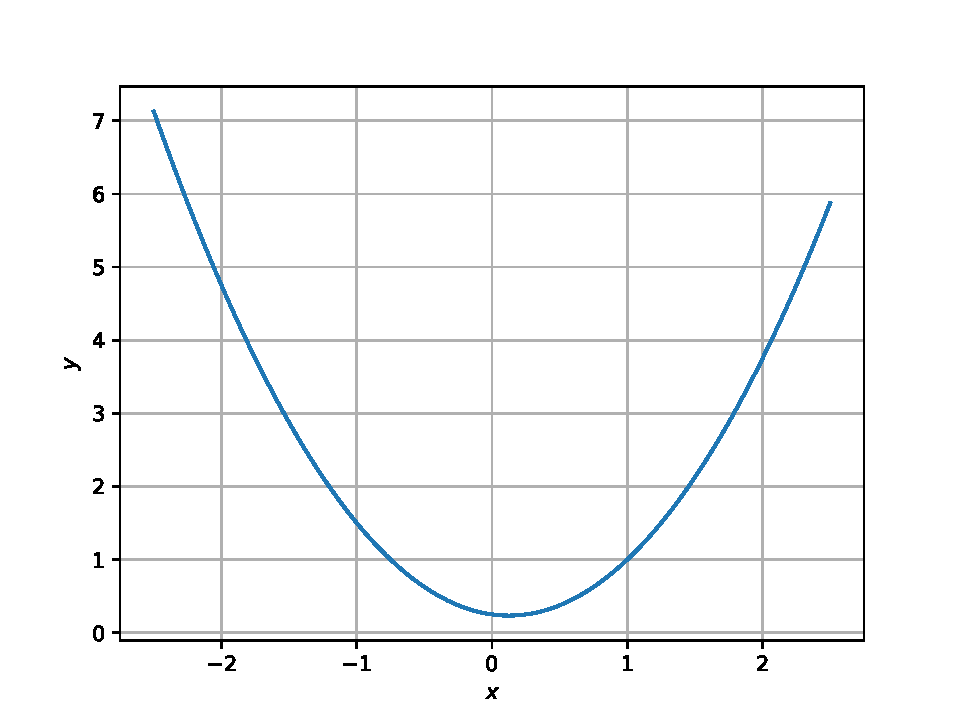
\includegraphics[width=\columnwidth]{./solutions/5/figs/conics/q20e.eps}
	\caption{}
	\label{fig:5.2.5_qtoe}	
	\end{figure}
		
 
Here, sum of zeroes = D = $\frac{1}{4}$\\
Product of zeroes = F = $\frac{1}{4}$\\
Substituing the values in \ref{eq:5.2.5_qtwenty},\\

\begin{multline}
\vec{x}^T\myvec{1&0\\0&0}\vec{x}  + \myvec{-\frac{1}{4}&-1}\vec{x} + \frac{1}{4} = 0
\end{multline}
\begin{align}
\implies y = x^2 - \frac{1}{4}x + \frac{1}{4} 
\end{align}
Since the curve doesn't meet the x-axis, real roots don't exist for this parabola as represented in Fig. \ref{fig:5.2.5_qtoe}	

		\item $\sqrt{2}$,$\frac{1}{3}$
	\begin{figure}[!ht]
	\centering
	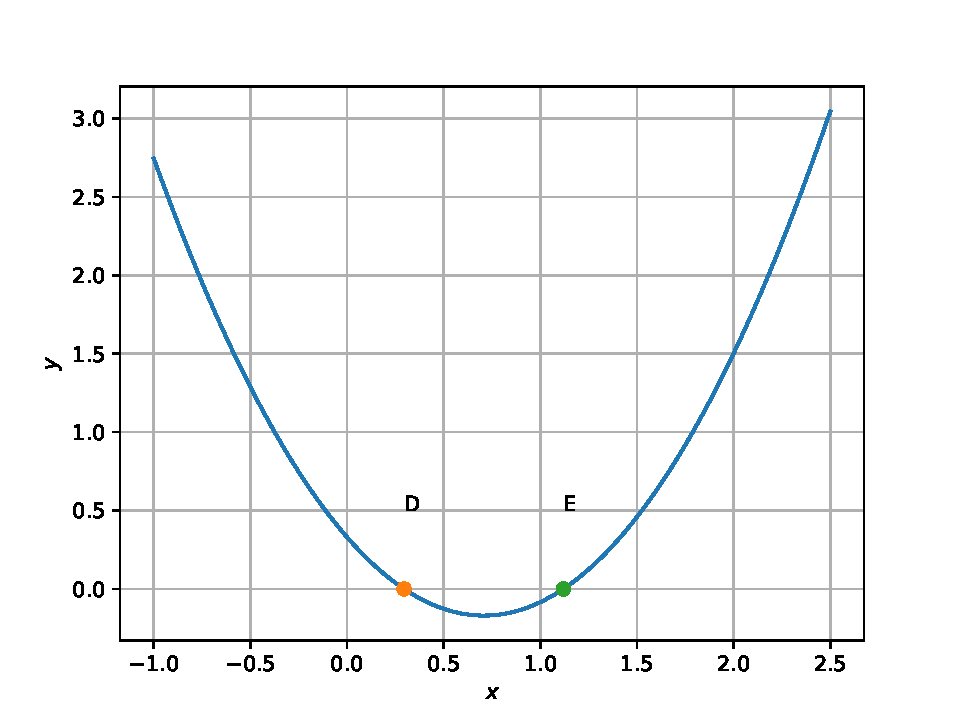
\includegraphics[width=\columnwidth]{./solutions/5/figs/conics/q20f.eps}
	\caption{}
	\label{fig:5.2.5_qtof}	
	\end{figure}

		

Here, sum of zeroes = D = $\sqrt{2}$\\
Product of zeroes = F = $\frac{1}{3}$\\
Substituing the values in \ref{eq:5.2.5_qtwenty},\\
\begin{multline}
\vec{x}^T\myvec{1&0\\0&0}\vec{x}  + \myvec{-\sqrt{2}&-1}\vec{x} + \frac{1}{3} = 0
\end{multline}
\begin{align}
\implies y = x^2 - \sqrt{2}x + \frac{1}{3}
\end{align}
The roots are 1.11 and 0.29 as represented in Fig. \ref{fig:5.2.5_qtof}
	\end{enumerate}

\item Find the roots of the following quadratic equations:
\begin{enumerate}
\item $x^2 – 3x – 10=0$
\item $2x^2+x-6=0$
\item $\sqrt{2}x^2 +7x+5\sqrt{2}  = 0$
\item $2x^2– x +\frac{1}{8} = 0 $
\item $100x^2 – 20x +1 = 0$
\end{enumerate}
\solution 
From theory, we understand that using dot product we can find the angle between the lines 
\begin{enumerate}
	\item 
	\begin{align}\label{eq:solutions/line_plane/74/codes:5}
		\frac{x-2}{2} = \frac{y-1}{5} &= \frac{z+3}{-3}, 
	\end{align}
	\begin{align}\label{eq:solutions/line_plane/74/codes:6}
		\frac{x+2}{-1} = \frac{y-4}{8} &= \frac{z-5}{4} 
	\end{align}


The above symmetric equations \ref{eq:solutions/line_plane/74/codes:5}, \ref{eq:solutions/line_plane/74/codes:6} can be represented in the vector form as 
\begin{align}\label{eq:solutions/line_plane/74/codes7}
	\quad \vec{r_1} &= \myvec{2\\1\\-3} + \lambda_1\myvec{2\\5\\-3}
	\\
	\quad \vec{r_2} &= \myvec{-2\\4\\5} + \lambda_2\myvec{-1\\8\\4}
\end{align}

As we have to find the angle between the vectors, we will only be taking the direction vectors into consideration. The direction vectors are $\vec{u}$ = $\myvec{2\\5\\-3}$ and $\vec{v}$ = $\myvec{-1\\8\\4}$. We can find the corresponding magnitude values

\begin{align}\label{eq:solutions/line_plane/74/codes9}
	\norm{\vec{u}} =\sqrt{2^{2}+5^{2}+(-3)^{2}} =\sqrt{38}
\end{align}
\begin{align}\label{eq:solutions/line_plane/74/codes10}
	\norm{\vec{v}} =\sqrt{(-1)^{2}+8^{2}+4^{2}} =\sqrt{81}
\end{align}

Using \ref{eq:solutions/line_plane/74/codes4}, \ref{eq:solutions/line_plane/74/codes9}, \ref{eq:solutions/line_plane/74/codes10} we get
\begin{align}
	\theta = \cos ^{-1}\frac{\myvec{2\\5\\-3}^{T}\myvec{-1\\8\\4}}{(\sqrt{38})(\sqrt{81})} 
	\\
	\theta = \cos ^{-1}\frac{26}{55.4797}
	\\
	\theta = \cos ^{-1} (0.4686)
	\\
	\theta = 62.053\degree
\end{align}

Therefore, the angle between the two lines is $62.053\degree$.See Fig. \ref{fig:solutions/line_plane/74/codesline_equation_1}

\begin{figure}
	\centering
	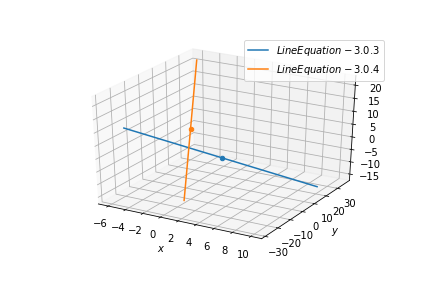
\includegraphics[width=\columnwidth]{./solutions/line_plane/74/codes/figs/Line_interest_1.png}
	\caption{Graph for equations \ref{eq:solutions/line_plane/74/codes7}}
	\label{fig:solutions/line_plane/74/codesline_equation_1}
\end{figure}


	\item 
	\begin{align}\label{eq:solutions/line_plane/74/codes12}
		\frac{x}{2} = \frac{y}{2} &= \frac{z}{1}, 
	\end{align}
	\begin{align}\label{eq:solutions/line_plane/74/codes13}
		\frac{x-5}{4} = \frac{y-2}{1} &= \frac{z-3}{8} 
	\end{align}



The above symmetric equations \ref{eq:solutions/line_plane/74/codes12}, \ref{eq:solutions/line_plane/74/codes13} can be represented in the vector form as 
\begin{align}\label{eq:solutions/line_plane/74/codes14}
	\quad \vec{r_1} &= \myvec{0\\0\\0} + \lambda_1\myvec{2\\2\\1}
	\\
	\quad \vec{r_2} &= \myvec{5\\2\\3} + \lambda_2\myvec{4\\1\\8}
\end{align}

As we have to find the angle between the vectors, we will only be taking the direction vectors into consideration. The direction vectors are $\vec{u}$ = $\myvec{2\\2\\1}$ and $\vec{v}$ = $\myvec{4\\1\\8}$. We can find the corresponding magnitude values

\begin{align}\label{eq:solutions/line_plane/74/codes16}
	\norm{\vec{u}} =\sqrt{2^{2}+2^{2}+1^{2}} =\sqrt{9}
\end{align}
\begin{align}\label{eq:solutions/line_plane/74/codes17}
	\norm{\vec{v}} =\sqrt{4^{2}+1^{2}+8^{2}} =\sqrt{81}
\end{align}

Using \ref{eq:solutions/line_plane/74/codes4}, \ref{eq:solutions/line_plane/74/codes16}, \ref{eq:solutions/line_plane/74/codes17} we get
\begin{align}
	\theta = \cos ^{-1}\frac{\myvec{2\\2\\1}^{T}\myvec{4\\1\\8}}{(\sqrt{9})(\sqrt{81})} 
	\\
	\theta = \cos ^{-1}\frac{18}{27.00}
	\\
	\theta = \cos ^{-1} (0.667)
	\\
	\theta = 48.189\degree
\end{align}

Therefore, the angle between the two lines is $48.189\degree$. See Fig. \ref{fig:solutions/line_plane/74/codesline_equation_2}


\begin{figure}
	\centering
	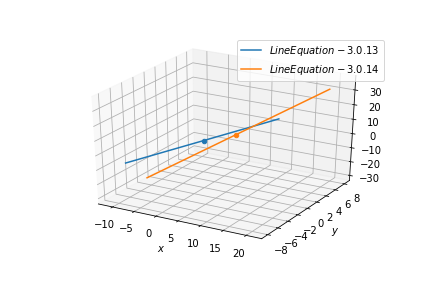
\includegraphics[width=\columnwidth]{./solutions/line_plane/74/codes/figs/Line_interest_2.png}
	\caption{Graph for equations \ref{eq:solutions/line_plane/74/codes14}}
	\label{fig:solutions/line_plane/74/codesline_equation_2}
\end{figure}
\end{enumerate}

    

\item Find the roots of the following quadratic equations
\begin{enumerate}
\item 	$2x^2-7x+3 = 0$
\item 	2$x^2+x-4 = 0$
\item 	$4x^2+4\sqrt{3}x+3 = 0$
\item 	2$x^2+x+4 = 0$
\end{enumerate}
\solution 
From theory, we understand that using dot product we can find the angle between the lines 
\begin{enumerate}
	\item 
	\begin{align}\label{eq:solutions/line_plane/74/codes:5}
		\frac{x-2}{2} = \frac{y-1}{5} &= \frac{z+3}{-3}, 
	\end{align}
	\begin{align}\label{eq:solutions/line_plane/74/codes:6}
		\frac{x+2}{-1} = \frac{y-4}{8} &= \frac{z-5}{4} 
	\end{align}


The above symmetric equations \ref{eq:solutions/line_plane/74/codes:5}, \ref{eq:solutions/line_plane/74/codes:6} can be represented in the vector form as 
\begin{align}\label{eq:solutions/line_plane/74/codes7}
	\quad \vec{r_1} &= \myvec{2\\1\\-3} + \lambda_1\myvec{2\\5\\-3}
	\\
	\quad \vec{r_2} &= \myvec{-2\\4\\5} + \lambda_2\myvec{-1\\8\\4}
\end{align}

As we have to find the angle between the vectors, we will only be taking the direction vectors into consideration. The direction vectors are $\vec{u}$ = $\myvec{2\\5\\-3}$ and $\vec{v}$ = $\myvec{-1\\8\\4}$. We can find the corresponding magnitude values

\begin{align}\label{eq:solutions/line_plane/74/codes9}
	\norm{\vec{u}} =\sqrt{2^{2}+5^{2}+(-3)^{2}} =\sqrt{38}
\end{align}
\begin{align}\label{eq:solutions/line_plane/74/codes10}
	\norm{\vec{v}} =\sqrt{(-1)^{2}+8^{2}+4^{2}} =\sqrt{81}
\end{align}

Using \ref{eq:solutions/line_plane/74/codes4}, \ref{eq:solutions/line_plane/74/codes9}, \ref{eq:solutions/line_plane/74/codes10} we get
\begin{align}
	\theta = \cos ^{-1}\frac{\myvec{2\\5\\-3}^{T}\myvec{-1\\8\\4}}{(\sqrt{38})(\sqrt{81})} 
	\\
	\theta = \cos ^{-1}\frac{26}{55.4797}
	\\
	\theta = \cos ^{-1} (0.4686)
	\\
	\theta = 62.053\degree
\end{align}

Therefore, the angle between the two lines is $62.053\degree$.See Fig. \ref{fig:solutions/line_plane/74/codesline_equation_1}

\begin{figure}
	\centering
	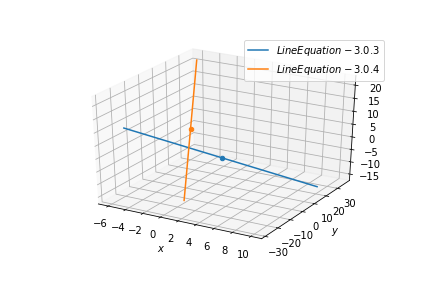
\includegraphics[width=\columnwidth]{./solutions/line_plane/74/codes/figs/Line_interest_1.png}
	\caption{Graph for equations \ref{eq:solutions/line_plane/74/codes7}}
	\label{fig:solutions/line_plane/74/codesline_equation_1}
\end{figure}


	\item 
	\begin{align}\label{eq:solutions/line_plane/74/codes12}
		\frac{x}{2} = \frac{y}{2} &= \frac{z}{1}, 
	\end{align}
	\begin{align}\label{eq:solutions/line_plane/74/codes13}
		\frac{x-5}{4} = \frac{y-2}{1} &= \frac{z-3}{8} 
	\end{align}



The above symmetric equations \ref{eq:solutions/line_plane/74/codes12}, \ref{eq:solutions/line_plane/74/codes13} can be represented in the vector form as 
\begin{align}\label{eq:solutions/line_plane/74/codes14}
	\quad \vec{r_1} &= \myvec{0\\0\\0} + \lambda_1\myvec{2\\2\\1}
	\\
	\quad \vec{r_2} &= \myvec{5\\2\\3} + \lambda_2\myvec{4\\1\\8}
\end{align}

As we have to find the angle between the vectors, we will only be taking the direction vectors into consideration. The direction vectors are $\vec{u}$ = $\myvec{2\\2\\1}$ and $\vec{v}$ = $\myvec{4\\1\\8}$. We can find the corresponding magnitude values

\begin{align}\label{eq:solutions/line_plane/74/codes16}
	\norm{\vec{u}} =\sqrt{2^{2}+2^{2}+1^{2}} =\sqrt{9}
\end{align}
\begin{align}\label{eq:solutions/line_plane/74/codes17}
	\norm{\vec{v}} =\sqrt{4^{2}+1^{2}+8^{2}} =\sqrt{81}
\end{align}

Using \ref{eq:solutions/line_plane/74/codes4}, \ref{eq:solutions/line_plane/74/codes16}, \ref{eq:solutions/line_plane/74/codes17} we get
\begin{align}
	\theta = \cos ^{-1}\frac{\myvec{2\\2\\1}^{T}\myvec{4\\1\\8}}{(\sqrt{9})(\sqrt{81})} 
	\\
	\theta = \cos ^{-1}\frac{18}{27.00}
	\\
	\theta = \cos ^{-1} (0.667)
	\\
	\theta = 48.189\degree
\end{align}

Therefore, the angle between the two lines is $48.189\degree$. See Fig. \ref{fig:solutions/line_plane/74/codesline_equation_2}


\begin{figure}
	\centering
	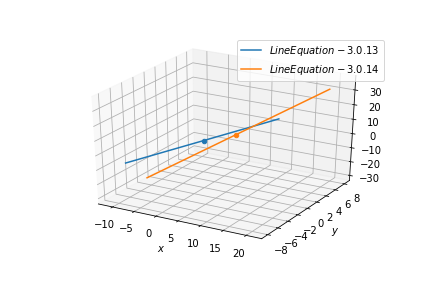
\includegraphics[width=\columnwidth]{./solutions/line_plane/74/codes/figs/Line_interest_2.png}
	\caption{Graph for equations \ref{eq:solutions/line_plane/74/codes14}}
	\label{fig:solutions/line_plane/74/codesline_equation_2}
\end{figure}
\end{enumerate}

    

\item Factorise $6x^2+ 17x + 5$.
\\
\solution 

The given polynomial can be expressed as:
\begin{align}
\vec{x}^T \myvec{6 & 0\\0 & 0}\vec{x}+ \myvec{17 & 0}\vec{x}+5=0
\end{align}
Substituting y=0 in the above equation,
\begin{align}
 6x^2+17x+5 &=0\\
\implies x&=\frac{-1}3{},\frac{-5}{2}\\
\therefore (3x+1)(2x+5) &=6x^2+17x+5
\end{align}
%
which is verified in Fig.     \ref{quadform/16/Fig:Graph Of $x^2+7x+10 &=$.}

\begin{figure}[ht!]
    \centering
    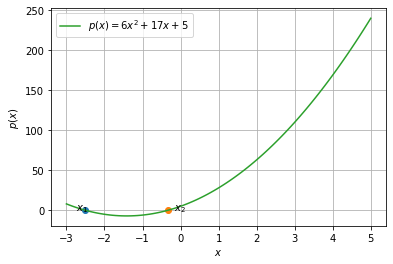
\includegraphics[width=\columnwidth]{solutions/su2021/2/16/Graph.png}
    \caption{Graph of $6x^2+17x+5$.}
    \label{quadform/16/Fig:Graph Of $x^2+7x+10 &=$.}
\end{figure}



\item Find the zeroes of the polynomial $x^2-3$ and verify the relationship between the zeroes and the coefficients.
\\
\solution 

\begin{table}[!ht]
\centering
\resizebox{\columnwidth}{!}{\begin{tabular}{|c|c|c|c|} 
\hline
kind of  cake & No.of cakes & Flour& Fat\\
\hline
1st & x & 200g  &  25g \\ 
\hline
2nd& y& 100g&  50g  \\ 
\hline
Total& x+y& 5 kg=5000g&1kg=1000g \\ 
\hline
\end{tabular}}
\caption{Ingredients used in making the cake is flour and fat }
\label{opt/13/tab:table1}
\end{table}
Let the  1st kind  be $x$ and the 2nd kind be $y$  such that 
\begin{align}
x \geq 0 \\
y \geq 0 
\end{align}
According to the question,
\begin{align}
2{x} + {y} \leq 50
\\
{x} + 2{y} \leq 40
\end{align}
$\therefore$ Our problem is
\begin{align}
\max_{\vec{x}} Z &= \myvec{1& 1}\vec{x}\\
s.t. \quad \myvec{2 & 1 \\ 1& 2}\vec{x} &\preceq \myvec{50\\40} 
\end{align}
Lagrangian function is given by
\begin{equation}
\begin{aligned}
&L(\vec{x},\boldsymbol{\lambda}) \\ &= \myvec{1 & 1}\vec{x}+\lcbrak{\sbrak{\myvec{2 & 1}\vec{x}-50}} \\ &+ \sbrak{\myvec{1 & 2}\vec{x}-40}\\ &+ \sbrak{\myvec{-1 & 0}\vec{x}} +\rcbrak{\sbrak{\myvec{0 & -1}\vec{x}}}\boldsymbol{\lambda}
\end{aligned}
\end{equation}
where,
\begin{align}
\boldsymbol{\lambda} &= \myvec{\lambda_1 \\ \lambda_2 \\ \lambda_3 \\ \lambda_4 \\ \lambda_5 \\ \lambda_6}
\end{align}
Now,
\begin{align}
\nabla L(\vec{x},\boldsymbol{\lambda}) &= \myvec{1+ \myvec{2 & 1 & -1 & 0 }\boldsymbol{\lambda}\\ 1+\myvec{1 & 2 & 0 & -1}\boldsymbol{\lambda} \\ \myvec{2 & 1}\vec{x}-50\\ \myvec{1& 2}\vec{x}-40 \\  \myvec{-1 & 0}\vec{x} \\ \myvec{0 & -1}\vec{x}}
\end{align}
$\therefore$ Lagrangian matrix is given by
\begin{align}
\myvec{0 & 0 & 2 & 1& -1 & 0 \\ 0 & 0 & 1 & 2  & 0 & -1 \\ 2 & 1 & 0 & 0 & 0 & 0 \\ 1 & 2 & 0 & 0 & 0 & 0  \\ -1 & 0 & 0 & 0 & 0 & 0  \\ 0 & -1 & 0 & 0 & 0 & 0 }\myvec{\vec{x} \\ \boldsymbol{\lambda} } &= \myvec{-1 \\ -1 \\ 50\\ 4 0\\ 0 \\0 }
\end{align}
Considering $\lambda_1,\lambda_2$ as only active multiplier,
\begin{align}
\myvec{0 & 0 & 2 & 1 \\ 0 & 0 & 1 & 2 \\ 2 & 1 & 0 & 0 \\ 1 & 2 & 0 & 0}\myvec{\vec{x}\\ \boldsymbol{\lambda}} &= \myvec{-1 \\ -1 \\ 5 0\\ 40}
\end{align}
resulting in,
\begin{align}
\myvec{\vec{x} \\ \boldsymbol{\lambda}} &= \myvec{0 & 0 & 2 & 1 \\ 0 & 0 & 1 & 2 \\ 2 & 1 & 0 & 0 \\ 1& 2 & 0 & 0}^{-1}\myvec{-1 \\ -1 \\ 50 \\ 40}
\\
\implies   \myvec{\vec{x} \\ \boldsymbol{\lambda}} &= \myvec{0 & 0 & \frac{2}{3} & \frac{-1}{3} \\ 0 & 0 & \frac{-1}{3} & \frac{2}{3} \\ \frac{2}{3} & \frac{-1}{3} & 0 & 0 \\ \frac{-1}{3} & \frac{2}{3} & 0 & 0}\myvec{-1 \\ -1 \\ 50 \\ 40}
\\
\implies \myvec{\vec{x} \\ \boldsymbol{\lambda}} &= \myvec{20 \\ 10 \\ -0.3 \\ -0.3 }
\end{align}
$\because \boldsymbol{\lambda}=\myvec{-0.3 \\ -0.3} \succ \vec{0} $
\\
$\therefore$ Optimal solution is given by
\begin{align}
    \vec{x} &= \myvec{20\\10} \\
    Z &= \myvec{1& 1}\vec{x} \\
    &= \myvec{1 & 1}\myvec{20 \\ 10} \\
    &= 60
\end{align}
By using cvxpy in python ,
\begin{align}
    \vec{x}=\myvec{20\\10}\\
    Z = 60
\end{align}
Hence No.of cakes \boxed{x=20} 1st kind and  .of cakes \boxed{y=10} 2nd kind should be used to maximum No. of cakes \boxed{Z=60}.  This is
verified in Fig. \ref{opt/13/fig: Graphical Solution}.	
%
\begin{figure}[!ht]
\centering
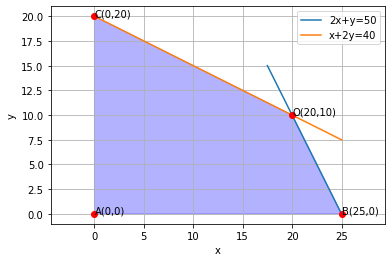
\includegraphics[width=\columnwidth]{solutions/su2021/2/13/Figure9.png}
\caption{Graphical Solution}
\label{opt/13/fig: Graphical Solution}	
\end{figure}

\item Find the discriminant of the quadratic equation $2x^2-4x+3 = 0$
hence find the nature of its roots.
\\
\solution

\begin{table}[!ht]
\centering
\resizebox{\columnwidth}{!}{\begin{tabular}{|c|c|c|c|} 
\hline
kind of  cake & No.of cakes & Flour& Fat\\
\hline
1st & x & 200g  &  25g \\ 
\hline
2nd& y& 100g&  50g  \\ 
\hline
Total& x+y& 5 kg=5000g&1kg=1000g \\ 
\hline
\end{tabular}}
\caption{Ingredients used in making the cake is flour and fat }
\label{opt/13/tab:table1}
\end{table}
Let the  1st kind  be $x$ and the 2nd kind be $y$  such that 
\begin{align}
x \geq 0 \\
y \geq 0 
\end{align}
According to the question,
\begin{align}
2{x} + {y} \leq 50
\\
{x} + 2{y} \leq 40
\end{align}
$\therefore$ Our problem is
\begin{align}
\max_{\vec{x}} Z &= \myvec{1& 1}\vec{x}\\
s.t. \quad \myvec{2 & 1 \\ 1& 2}\vec{x} &\preceq \myvec{50\\40} 
\end{align}
Lagrangian function is given by
\begin{equation}
\begin{aligned}
&L(\vec{x},\boldsymbol{\lambda}) \\ &= \myvec{1 & 1}\vec{x}+\lcbrak{\sbrak{\myvec{2 & 1}\vec{x}-50}} \\ &+ \sbrak{\myvec{1 & 2}\vec{x}-40}\\ &+ \sbrak{\myvec{-1 & 0}\vec{x}} +\rcbrak{\sbrak{\myvec{0 & -1}\vec{x}}}\boldsymbol{\lambda}
\end{aligned}
\end{equation}
where,
\begin{align}
\boldsymbol{\lambda} &= \myvec{\lambda_1 \\ \lambda_2 \\ \lambda_3 \\ \lambda_4 \\ \lambda_5 \\ \lambda_6}
\end{align}
Now,
\begin{align}
\nabla L(\vec{x},\boldsymbol{\lambda}) &= \myvec{1+ \myvec{2 & 1 & -1 & 0 }\boldsymbol{\lambda}\\ 1+\myvec{1 & 2 & 0 & -1}\boldsymbol{\lambda} \\ \myvec{2 & 1}\vec{x}-50\\ \myvec{1& 2}\vec{x}-40 \\  \myvec{-1 & 0}\vec{x} \\ \myvec{0 & -1}\vec{x}}
\end{align}
$\therefore$ Lagrangian matrix is given by
\begin{align}
\myvec{0 & 0 & 2 & 1& -1 & 0 \\ 0 & 0 & 1 & 2  & 0 & -1 \\ 2 & 1 & 0 & 0 & 0 & 0 \\ 1 & 2 & 0 & 0 & 0 & 0  \\ -1 & 0 & 0 & 0 & 0 & 0  \\ 0 & -1 & 0 & 0 & 0 & 0 }\myvec{\vec{x} \\ \boldsymbol{\lambda} } &= \myvec{-1 \\ -1 \\ 50\\ 4 0\\ 0 \\0 }
\end{align}
Considering $\lambda_1,\lambda_2$ as only active multiplier,
\begin{align}
\myvec{0 & 0 & 2 & 1 \\ 0 & 0 & 1 & 2 \\ 2 & 1 & 0 & 0 \\ 1 & 2 & 0 & 0}\myvec{\vec{x}\\ \boldsymbol{\lambda}} &= \myvec{-1 \\ -1 \\ 5 0\\ 40}
\end{align}
resulting in,
\begin{align}
\myvec{\vec{x} \\ \boldsymbol{\lambda}} &= \myvec{0 & 0 & 2 & 1 \\ 0 & 0 & 1 & 2 \\ 2 & 1 & 0 & 0 \\ 1& 2 & 0 & 0}^{-1}\myvec{-1 \\ -1 \\ 50 \\ 40}
\\
\implies   \myvec{\vec{x} \\ \boldsymbol{\lambda}} &= \myvec{0 & 0 & \frac{2}{3} & \frac{-1}{3} \\ 0 & 0 & \frac{-1}{3} & \frac{2}{3} \\ \frac{2}{3} & \frac{-1}{3} & 0 & 0 \\ \frac{-1}{3} & \frac{2}{3} & 0 & 0}\myvec{-1 \\ -1 \\ 50 \\ 40}
\\
\implies \myvec{\vec{x} \\ \boldsymbol{\lambda}} &= \myvec{20 \\ 10 \\ -0.3 \\ -0.3 }
\end{align}
$\because \boldsymbol{\lambda}=\myvec{-0.3 \\ -0.3} \succ \vec{0} $
\\
$\therefore$ Optimal solution is given by
\begin{align}
    \vec{x} &= \myvec{20\\10} \\
    Z &= \myvec{1& 1}\vec{x} \\
    &= \myvec{1 & 1}\myvec{20 \\ 10} \\
    &= 60
\end{align}
By using cvxpy in python ,
\begin{align}
    \vec{x}=\myvec{20\\10}\\
    Z = 60
\end{align}
Hence No.of cakes \boxed{x=20} 1st kind and  .of cakes \boxed{y=10} 2nd kind should be used to maximum No. of cakes \boxed{Z=60}.  This is
verified in Fig. \ref{opt/13/fig: Graphical Solution}.	
%
\begin{figure}[!ht]
\centering
\includegraphics[width=\columnwidth]{solutions/su2021/2/13/Figure9.png}
\caption{Graphical Solution}
\label{opt/13/fig: Graphical Solution}	
\end{figure}

\item Find the discriminant of the quadratic equation $3x^2-2x+\frac{1}{3} = 0$
hence find the nature of its roots.
\\
\solution

The given equation can be expressed as
\begin{align}
\vec{x}^T \myvec{3 & 0\\0 & 0}\vec{x}+ 2\myvec{-1 \\ \frac{-1}{2}}\vec{x}+\frac{1}{3}=0
\end{align}
with
\begin{align}
\vec{V} = \myvec{3 & 0 \\ 0 & 0},\vec{u}=\myvec{-1 \\ \frac{-1}{2}},f=\frac{1}{3}
\end{align}
Using eigenvalue decomposition,
\begin{align}
\vec{D} = \myvec{0 & 0\\0 & 3} ,\vec{P}=\myvec{0 & 1\\1 & 0}
\end{align}
Thus,
\begin{align}
\myvec{\vec{u}^T + \eta\vec{p_1}^T \\ \vec{V}}\vec{c} &= \myvec{-f \\ \eta\vec{p_1}-\vec{u}} 
\\
\implies \myvec{-1 & -1 \\ 3 & 0 \\ 0 & 0}\vec{c} &= \myvec{\frac{-1}{3}\\ 1 \\ 0} \\
\implies  \myvec{-1 & -1 \\ 3 & 0}\vec{c} &= \myvec{\frac{-1}{3}\\ 1}
\\
\implies \vec{c} &= \myvec{\frac{1}{3}\\0}
\end{align}
$\because$
\begin{align}
\vec{p_1}^T\vec{c} &= \myvec{0 & 1}\myvec{\frac{1}{3}\\0}
\\
&= 0
\\
\vec{p_2}^T\vec{V}\vec{p_2} &= \myvec{1 & 0}\myvec{3 & 0\\0& 0}\myvec{1 \\ 0}
\\
&= 3,
\end{align}
$\because$
\begin{align}
(\vec{p_1}^T\vec{c})(\vec{p_2}^T\vec{V}\vec{p_2}) = 0
\end{align}
Thus, the given equation has  real and equal roots which can be verified from Fig. \ref{quadforms/2/25/Roots of}.  
%
\begin{figure}[!ht]
\centering
\includegraphics[width=\columnwidth]{solutions/su2021/2/25/download (3).png}
\caption{Roots of $3x^2 -2x + 1/3 = 0$ }
\label{quadforms/2/25/Roots of}
\end{figure}






\item Find the equation of all lines having slope 2 and being tangent to the curve
\begin{align}
y + \frac{2}{x-3} = 0
\end{align}
%
\\
\solution

The equation of curve can be expressed as 
\begin{align}
  y+\frac{2}{x-3}=0  \\
  xy-3y+2=0\label{quadform/41/eq:giveneq}
\end{align}
Comparing with the standard equation, 
\begin{align}
\vec{x}^T\vec{V}\vec{x}+2\vec{u}^T\vec{x}+f=0\\
\vec{V}=\myvec{0&\frac{1}{2}\\\frac{1}{2}&0},\vec{u}=\myvec{0\\-\frac{3}{2}},f=2\\
\vec{V}^{-1}=\myvec{0&2\\2&0}
\end{align}
$\because$
\begin{align}
    \abs{\vec{V}} &= \frac{-1}{4}
    \\
    \implies \abs{\vec{V}} &< 0
\end{align}
and \eqref{quadform/41/eq:giveneq} represents a hyperbola.
The characteristic equation of $\vec{V}$ is 
\begin{align}
    \abs{\vec{V} - \lambda\vec{I}} = \mydet{-\lambda & \frac{1}{2} \\ \frac{1}{2} & -\lambda} &= 0
    \\
    \implies \lambda^2 - \frac{1}{4} &= 0
\end{align}
and the eigenvalues are 
\begin{align}
    \lambda_1 = \frac{1}{2} , \lambda_2 = \frac{-1}{2}
\end{align}
% Eigen vector $\vec{p}$ is 
% \begin{align}
%     \vec{V}\vec{p} &= \lambda\vec{p}
%     \\
%     \implies (\vec{V} - \lambda\vec{I})\vec{p} &= 0
% \end{align}
Eigen vector $\vec{p}_1$ corressponding to $\lambda_1$ can be obtained as
\begin{align}
    (\vec{V} - \lambda_1\vec{I}) &= \myvec{\frac{-1}{2} & \frac{1}{2} \\ \frac{1}{2} & \frac{-1}{2}}\xleftrightarrow[R_1 \leftarrow -2R_1]{R_2 = R_1 + R_2}\myvec{1 & -1 \\ 0 & 0}
    \\
    \implies \vec{p_1} &= \frac{1}{\sqrt{2}}\myvec{1 \\ 1}
\end{align}
Similarly,
\begin{align}
    \vec{p_2} &= \frac{1}{\sqrt{2}}\myvec{-1 \\ 1}
\end{align}
$\therefore$
\begin{align}
    \vec{P} &= \myvec{\vec{p_1} & \vec{p_2}} = \frac{1}{\sqrt{2}}\myvec{1 & -1 \\ 1 & 1}
    \\
    \vec{D} &= \myvec{\lambda_1 & 0 \\ 0 & \lambda_2} = \myvec{\frac{1}{2} & 0 \\ 0 & \frac{-1}{2}}
\end{align}
Now,
\begin{align}
    \vec{c} &= -\vec{V}^{-1}\vec{u} 
    \\
    &= -\myvec{0 & 2 \\2 & 0}\myvec{0 \\ \frac{-3}{2}}
    \\
    &= \myvec{3 \\ 0}
\end{align}
\begin{align}
\because \vec{u}^T\vec{V}^{-1}\vec{u} - f<0,
\end{align}
the axes need to be swapped and 
\begin{align}
    \sqrt{\frac{ \vec{u}^T\vec{V}^{-1}\vec{u} - f}{\lambda_2}} &= 2
    \\
    \sqrt{ \frac{f- \vec{u}^T\vec{V}^{-1}\vec{u}}{\lambda_1}} &= 2
\end{align}
$\therefore$ the equation of the standard hyperbola can be expressed as 
\begin{align}
    \frac{y^2}{4} - \frac{x^2}{4} &= 1
\end{align}
The direction and normal vectors of tangent with slope 2 are 
\begin{align}
    \vec{m}=\myvec{1\\2},\vec{n}=\myvec{-2\\1}
\end{align}
From the  conics table in the manual,
\begin{align}
\kappa = \pm \sqrt{\frac{\vec{u}^T\vec{V}^{-1}\vec{u}-f}{\vec{n}^T\vec{V}^{-1}\vec{n}}} = \pm \sqrt{\frac{1}{4}} = \pm \frac{1}{2}
\end{align}
and the desired points of contact are 
\begin{align}
\vec{q}&=\vec{V}^{-1}(\kappa\vec{n}-\vec{u})\\
\implies \vec{q}_1=\myvec{4\\-2}, 
\vec{q}_2=\myvec{2\\2}\label{quadform/41/eq:10}
\end{align}
The equation of the tangents are given by
\begin{align}
    \vec{n}^T\vec{x}&=\vec{n}^T\vec{q}\\
    \implies \myvec{-2&1}\vec{x}&=\myvec{-2&1}\myvec{4\\-2}=-10\\
    \text{and }\myvec{-2&1}\vec{x}&=\myvec{-2&1}\myvec{2\\2}=-2
\end{align}
%
The above results are verified in Fig. \ref{quadform/41/fig:tangents}.	
\begin{figure}[!ht]
\centering
\includegraphics[width=\columnwidth]{solutions/su2021/2/41/figure6_1.png}
\caption{The tangents to the curve with slope 2 }
\label{quadform/41/fig:tangents}	
\end{figure}




\item Find the point at which the tangent to the curve $y = \sqrt{4x-3}-1$ has its 
slope $\frac{2}{3}$.
%
\\
\solution
Given curve,
\begin{align}
y = \sqrt{4x-3}-1\label{quadform/42/2.0.1}\\
\implies (y+1)^2 =4x-3\\
\implies y^2-4x+2y+4 =0
\end{align}
which has the vector parameters
\begin{align}
\vec{V}&=\myvec{0 & 0 \\ 0 & 1},\vec{u}=\myvec{-2 & 1 }, \vec{f} = 4 
\end{align}
\begin{align}
|\vec{V}| = 0
\end{align}
$\therefore $ the given curve \eqref{quadform/42/2.0.1} is parabola. In standard form,
\begin{align}
\vec{P} =\vec{I}\implies \vec{p_1} = \myvec{1 \\ 0}
\end{align}
Since the slope of the tangents is $\frac{2}{3}$, the direction and normal vectors are
\begin{align}
\vec{m} &= \myvec{1\\\frac{2}{3}}= \myvec{3\\2},\vec{n} = \myvec{2\\-3}\\
\text{and }
\kappa &= \frac{\vec{p_1^T}\vec{u}}{\vec{p_1^T}\vec{n}} = -1
\end{align}
$\therefore$ Point of contact for the tangent is
\begin{align}
  \myvec{\vec{u}+\kappa \vec{n^T}\\\vec{V} }\vec{q} &= \myvec{\vec{-f}\\\kappa \vec{n} -\vec{u}}\\
  \implies\myvec{-4 & 4\\0 & 0 \\0 & 1} \vec{q}&= \myvec{-4\\0\\2}\\
  \implies \vec{q}&=\myvec{3\\2}
\end{align}
%$\therefore $ Point of contact for tangent of given curve is
% \begin{align}
% \vec{q }= \myvec{3\\2}
% \end{align}
which is verified in Fig.     \ref{quadform/42/fig:Tangent to parabola.}
%
\begin{figure}[ht]
    \centering
    \includegraphics[width=\columnwidth]{solutions/su2021/2/42/PARABOLA.png}
    \caption{Tangent to Parabola.}
    \label{quadform/42/fig:Tangent to parabola.}
\end{figure}    



\item Find the equation of the normal to the curve $x^2= 4y$
which passes through the point \myvec{1\\ 2}.
%
\solution
The given curve can be expressed as 
\begin{align}
 x^2-4y &=0 \label{quadform/45/2.0.2}
 \\
%\vec{x}^T\vec{V}\vec{x}+2\vec{u}^T\vec{x}+f=0\\
\implies \vec{V}=\myvec{1 & 0 \\ 0 & 0},\vec{u}=\myvec{0 \\ -2 }, \vec{f} = 0 
\end{align}
$\because$
\begin{align}
 \abs{\vec{V}} &= 0
\end{align}
the given curve \eqref{quadform/45/2.0.2} represents a parabola.
The eigenvalues are given by 
\begin{align}
\lambda_1 = 0 , \lambda_2 = 1
\end{align}
with corresponding eigenvectors
\begin{align}
\myvec{1 & 0 \\ 0 & 0}\vec{x} &=0 \implies \vec{p_1} = \myvec{0 \\ 1}
\\
\myvec{0 & 0 \\ 0 & -1}\vec{x} &=0 \implies \vec{p_2} = \myvec{1 \\ 0}
\end{align}
To find the vertex of the parabola ,
\begin{align} \myvec{\vec{u^T}+\kappa\vec{p_1^T}\\\vec{V} }\vec{c} &= \myvec{\vec{-f}\\\kappa \vec{p_1} -\vec{u}}
\\
\text{where, }  \kappa = \vec{u^T}\vec{p_1} = -2
\\
\implies\myvec{0 & -4\\1 & 0 \\0 & 0} \vec{c}&= \myvec{0\\0\\0} \label{quadform/45/eq:b}
\end{align}
from the above it can be observed that,
\begin{align}    
   \vec{c} &= \myvec{0 \\ 0}
\end{align}
Now to evalute the direction vector m,
\begin{align}
\vec{m}^T(\vec{V}\vec{q} + \vec{u}) &=0
\\
\implies \vec{m}^T\brak{\myvec{1 & 0 \\ 0 & 0}\myvec{1 \\ 2} + \myvec{0 \\ -2}} &=0
\\
\implies \vec{m}^T\myvec{1 \\ -2} &=0
\\
\implies \vec{m} = \myvec{-2 \\ -1}
\end{align}
The normal is obtained as 
\begin{align}
\vec{m}^T(\vec{x} - \vec{q}) &=0 
\\
\myvec{-2 & -1}\brak{\vec{x}-\myvec{1 \\ 2}} &= 0
\\
\myvec{-2 & -1}\vec{x}+ 4 &= 0 
\end{align}
%
The above results are verified in Fig.     \ref{quadform/45/fig:Normal to parabola.}.
\begin{figure}[ht]
    \centering
    \includegraphics[width=\columnwidth]{solutions/su2021/2/45/FIGURE4.png}
    \caption{Normal to Parabola.}
    \label{quadform/45/fig:Normal to parabola.}
\end{figure}    


%
\item Find the intervals in which the function 
\begin{align}
f(x)  = x^2-4x+6
\end{align}
%
is 
\begin{enumerate}
\item increasing
\item decreasing.
\end{enumerate}
%
\solution

\begin{table}[!ht]
\centering
\resizebox{\columnwidth}{!}{\begin{tabular}{|c|c|c|c|} 
\hline
kind of  cake & No.of cakes & Flour& Fat\\
\hline
1st & x & 200g  &  25g \\ 
\hline
2nd& y& 100g&  50g  \\ 
\hline
Total& x+y& 5 kg=5000g&1kg=1000g \\ 
\hline
\end{tabular}}
\caption{Ingredients used in making the cake is flour and fat }
\label{opt/13/tab:table1}
\end{table}
Let the  1st kind  be $x$ and the 2nd kind be $y$  such that 
\begin{align}
x \geq 0 \\
y \geq 0 
\end{align}
According to the question,
\begin{align}
2{x} + {y} \leq 50
\\
{x} + 2{y} \leq 40
\end{align}
$\therefore$ Our problem is
\begin{align}
\max_{\vec{x}} Z &= \myvec{1& 1}\vec{x}\\
s.t. \quad \myvec{2 & 1 \\ 1& 2}\vec{x} &\preceq \myvec{50\\40} 
\end{align}
Lagrangian function is given by
\begin{equation}
\begin{aligned}
&L(\vec{x},\boldsymbol{\lambda}) \\ &= \myvec{1 & 1}\vec{x}+\lcbrak{\sbrak{\myvec{2 & 1}\vec{x}-50}} \\ &+ \sbrak{\myvec{1 & 2}\vec{x}-40}\\ &+ \sbrak{\myvec{-1 & 0}\vec{x}} +\rcbrak{\sbrak{\myvec{0 & -1}\vec{x}}}\boldsymbol{\lambda}
\end{aligned}
\end{equation}
where,
\begin{align}
\boldsymbol{\lambda} &= \myvec{\lambda_1 \\ \lambda_2 \\ \lambda_3 \\ \lambda_4 \\ \lambda_5 \\ \lambda_6}
\end{align}
Now,
\begin{align}
\nabla L(\vec{x},\boldsymbol{\lambda}) &= \myvec{1+ \myvec{2 & 1 & -1 & 0 }\boldsymbol{\lambda}\\ 1+\myvec{1 & 2 & 0 & -1}\boldsymbol{\lambda} \\ \myvec{2 & 1}\vec{x}-50\\ \myvec{1& 2}\vec{x}-40 \\  \myvec{-1 & 0}\vec{x} \\ \myvec{0 & -1}\vec{x}}
\end{align}
$\therefore$ Lagrangian matrix is given by
\begin{align}
\myvec{0 & 0 & 2 & 1& -1 & 0 \\ 0 & 0 & 1 & 2  & 0 & -1 \\ 2 & 1 & 0 & 0 & 0 & 0 \\ 1 & 2 & 0 & 0 & 0 & 0  \\ -1 & 0 & 0 & 0 & 0 & 0  \\ 0 & -1 & 0 & 0 & 0 & 0 }\myvec{\vec{x} \\ \boldsymbol{\lambda} } &= \myvec{-1 \\ -1 \\ 50\\ 4 0\\ 0 \\0 }
\end{align}
Considering $\lambda_1,\lambda_2$ as only active multiplier,
\begin{align}
\myvec{0 & 0 & 2 & 1 \\ 0 & 0 & 1 & 2 \\ 2 & 1 & 0 & 0 \\ 1 & 2 & 0 & 0}\myvec{\vec{x}\\ \boldsymbol{\lambda}} &= \myvec{-1 \\ -1 \\ 5 0\\ 40}
\end{align}
resulting in,
\begin{align}
\myvec{\vec{x} \\ \boldsymbol{\lambda}} &= \myvec{0 & 0 & 2 & 1 \\ 0 & 0 & 1 & 2 \\ 2 & 1 & 0 & 0 \\ 1& 2 & 0 & 0}^{-1}\myvec{-1 \\ -1 \\ 50 \\ 40}
\\
\implies   \myvec{\vec{x} \\ \boldsymbol{\lambda}} &= \myvec{0 & 0 & \frac{2}{3} & \frac{-1}{3} \\ 0 & 0 & \frac{-1}{3} & \frac{2}{3} \\ \frac{2}{3} & \frac{-1}{3} & 0 & 0 \\ \frac{-1}{3} & \frac{2}{3} & 0 & 0}\myvec{-1 \\ -1 \\ 50 \\ 40}
\\
\implies \myvec{\vec{x} \\ \boldsymbol{\lambda}} &= \myvec{20 \\ 10 \\ -0.3 \\ -0.3 }
\end{align}
$\because \boldsymbol{\lambda}=\myvec{-0.3 \\ -0.3} \succ \vec{0} $
\\
$\therefore$ Optimal solution is given by
\begin{align}
    \vec{x} &= \myvec{20\\10} \\
    Z &= \myvec{1& 1}\vec{x} \\
    &= \myvec{1 & 1}\myvec{20 \\ 10} \\
    &= 60
\end{align}
By using cvxpy in python ,
\begin{align}
    \vec{x}=\myvec{20\\10}\\
    Z = 60
\end{align}
Hence No.of cakes \boxed{x=20} 1st kind and  .of cakes \boxed{y=10} 2nd kind should be used to maximum No. of cakes \boxed{Z=60}.  This is
verified in Fig. \ref{opt/13/fig: Graphical Solution}.	
%
\begin{figure}[!ht]
\centering
\includegraphics[width=\columnwidth]{solutions/su2021/2/13/Figure9.png}
\caption{Graphical Solution}
\label{opt/13/fig: Graphical Solution}	
\end{figure}

\item Find the equation of the parabola with focus \myvec{2\\0} and directrix $\myvec{1 & 0}\vec{x} = -2$.\item Find the equation of the parabola with vertex at \myvec{0\\ 0} and focus at \myvec{0\\ 2}.
\\
\solution
% The equation of a plane $P$ passing through the line of intersection of the planes $P_{1}$ and $P_{2}$ has the form,
% \begin{align}
%    P : P_{1} + \lambda P_{2}\label{sep/2/28eq1}
% \end{align}
% %
% General equation of plane is given by
% \begin{align}
%     \vec{n}^T\vec{x}=c
% \end{align}
% Where $\vec{n}$ is normal vector to the plane
\begin{lemma}
   The equation of a plane passing through intersection of planes
   \begin{align}
    \vec{n_{1}}^T\vec{x}&=c_{1}\\ \vec{n_{2}}^T\vec{x}&=c_{2}
   \end{align}
   and perpendicular to plane
   \begin{align}
     \vec{n_{3}}^T\vec{x}&=c_{3}
   \end{align}
   is given by 
   \begin{align}
      \vec{n_{4}}^T\vec{x}&=c_{4}
   \end{align}
   where 
   \begin{align}
       \vec{n_{4}} = \vec{n_{1}} - \brak{\frac{\vec{n_{3}^T\vec{n_1}}}{\vec{n_{3}^T\vec{n_2}}}}\vec{n_2}\\
       c_{4} = c_{1} - \brak{\frac{\vec{n_{3}^T\vec{n_1}}}{\vec{n_{3}^T\vec{n_2}}}}c_{2}
   \end{align}
\end{lemma}
\begin{proof}
   Let $P$ be the plane that passes through intersection 2 given planes.\\  From \eqref{sep/2/28/eq1}, equation of $P$ has the form,
   \begin{align}
       \vec{n_{1}}^T\vec{x} + \lambda\brak{\vec{n_{2}}^T\vec{x}} = c_{1} + \lambda\brak{c_{2}}\\
       \implies \brak{\vec{n_{1}}+\lambda\vec{n_{2}}}^T\vec{x} = c_{1} + \lambda\brak{c_{2}}
   \end{align}
  Normal vector to plane $P$ is,
 \begin{align}
     \vec{n_{4}} = \vec{n_{1}}+\lambda\vec{n_{2}}
 \end{align}
 As $P$ is perpendicular to the third plane i.e. angle between normal vectors is $90\degree$, 
 \begin{align}
     &\cos\brak{90\degree} = 0 = \dfrac{\vec{n_{3}}^T\vec{n_{4}}}{\norm{\vec{n_{3}}}\norm{\vec{n_{4}}}}\\
    \implies &\vec{n_{3}}^T\vec{n_{4}} = 0\\
    \implies &\vec{n_{3}}^T\brak{\vec{n_{1}}+\lambda\vec{n_{2}}} = 0\\
    \implies &\lambda = \frac{-\vec{n_{3}^T\vec{n_1}}}{\vec{n_{3}^T\vec{n_2}}}
 \end{align}
 Therefore equation of plane $P$ is,
 \begin{align}
     \brak{\vec{n_{1}} - \brak{\frac{\vec{n_{3}^T\vec{n_1}}}{\vec{n_{3}^T\vec{n_2}}}}\vec{n_2}}^T\vec{x} = c_{1} - \brak{\frac{\vec{n_{3}^T\vec{n_1}}}{\vec{n_{3}^T\vec{n_2}}}}c_{2}
 \end{align}
\end{proof}
For the given problem,
\begin{align}
  \vec{n_{1}}=\myvec{1\\1\\1}\\c_{1}=1,
  \vec{n_{2}}=\myvec{2\\3\\4},
     c_{2}=5\\
  \vec{n_{3}}=\myvec{1\\-1\\1}\\c_{3}=0 
 \end{align}
Solving the above we get,
\begin{align}
    \lambda = \frac{-1}{3},
    \vec{n_{4}} = \myvec{\frac{1}{3}\\0\\\frac{-1}{3}},
    c_{4} = \frac{-2}{3}
\end{align}
We have equation of the plane as,
\begin{align}
    \myvec{\frac{1}{3}&0&\frac{-1}{3}}\vec{x} = \frac{-2}{3} 
\end{align}
\begin{figure}[!ht]
\includegraphics[ width=\columnwidth]{solutions/sep/2/28/figures/planes.png}
\caption{Plane $P$ passing through intersection of $P_{1}$ and $P_{2}$ and perpendicular to $P_{3}$}
\label{sep/2/28fig:Line }	
\end{figure}

%
\item Find the equation of the ellipse, with major axis along the x-axis and passing through the points \myvec{4\\ 3} and \myvec{– 1\\4}.
\\
\solution
%
Given ellipse is
\begin{align}
   \vec{x}^T\myvec{9&0\\0&4}\vec{x}=36
\end{align}
%
On comparing it with standard form we have,
\begin{align}
    \vec{V}=\myvec{9&0\\0&4},\vec{u}=0,f=-36\\
    \implies\vec{u}^T\vec{V}^{-1}\vec{u}-f = 36\\
    \implies\vec{c} = -\vec{V}^{-1}\vec{u} = \myvec{0\\0}\\
\end{align}
The eigen vector decomposition of 
\begin{align}
    \vec{V} = \myvec{9&0\\0&4}
\end{align}
is given by
\begin{align}
    \vec{D} &= \myvec{9&0\\0&4} \implies \lambda_1 = 9,\lambda_2 = 4\\
    \vec{P} &= \myvec{1&0\\0&1}\implies \vec{p}_1 = \myvec{1\\0}, \vec{p}_2 = \myvec{0\\1}
\end{align}
Since
\begin{align}
   \lambda_1 > \lambda_2
\end{align}
Eccentricity of the ellipse is,
\begin{align}
   e &= \sqrt{1-\frac{\lambda_2}{\lambda_1}}
   = \frac{\sqrt{5}}{3}
\end{align} 
Semi major and minor axes of ellipse are,
\begin{align}
    a = \sqrt{\frac{\vec{u}^{\top}\vec{V}^{-1}\vec{u}-f}{\lambda_2}} = 3\\ 
    b = \sqrt{\frac{\vec{u}^{\top}\vec{V}^{-1}\vec{u}-f}{\lambda_1}} = 2
\end{align}
The co-ordinates of vertices are,
\begin{align}
   \pm\myvec{0 \\ 3} 
\end{align}
The co-ordinates of foci are given by,
\begin{align}
  \vec{F}  = \frac{ce^2\vec{n}-\vec{u}}{\lambda_1}
\end{align}
Where,
\begin{align}
    \vec{n} &= \sqrt{\lambda_1}\vec{p}_2
\end{align}
\begin{multline}
     c = \frac{e\vec{u}^{\top}\vec{n} \pm \sqrt{e^2\brak{\vec{u}^{\top}\vec{n}}^2-\lambda_2\brak{e^2-1}\brak{\norm{\vec{u}}^2 - \lambda_2 f}}}{\lambda_2e\brak{e^2-1}} 
\end{multline}
Substituting we have,
\begin{align}
    \vec{n} &= \myvec{0\\3}\\ c &= \pm\frac{27}{\sqrt{5}}\\
    \vec{F} &= \pm\myvec{0 \\ \sqrt{5}}.
\end{align}
See Fig.   \ref{sep/2/27/fig:RSUencountered}. 
\begin{figure}[t!]
  \centering
  \includegraphics[ width=\columnwidth]{solutions/sep/2/27/figures/ellipse.png}
  \caption{Plot of the ellipse}   
  \label{sep/2/27/fig:RSUencountered} 
\end{figure}

\item Find the coordinates of the foci and the vertices, the eccentricity,the length of the latus rectum of the hyperbolas
\begin{enumerate}
\item 
$
\vec{x}^T\myvec{\frac{1}{9} & 0 \\ 0 & -\frac{1}{16}}\vec{x} = 1
$
\item 
$
\vec{x}^T\myvec{1 & 0 \\ 0 & -16}\vec{x} = 16
$
\end{enumerate}
\solution
\begin{enumerate}
    \item 
    
\begin{table}[!ht]
\centering
\resizebox{\columnwidth}{!}{\begin{tabular}{|c|c|c|c|} 
\hline
kind of  cake & No.of cakes & Flour& Fat\\
\hline
1st & x & 200g  &  25g \\ 
\hline
2nd& y& 100g&  50g  \\ 
\hline
Total& x+y& 5 kg=5000g&1kg=1000g \\ 
\hline
\end{tabular}}
\caption{Ingredients used in making the cake is flour and fat }
\label{opt/13/tab:table1}
\end{table}
Let the  1st kind  be $x$ and the 2nd kind be $y$  such that 
\begin{align}
x \geq 0 \\
y \geq 0 
\end{align}
According to the question,
\begin{align}
2{x} + {y} \leq 50
\\
{x} + 2{y} \leq 40
\end{align}
$\therefore$ Our problem is
\begin{align}
\max_{\vec{x}} Z &= \myvec{1& 1}\vec{x}\\
s.t. \quad \myvec{2 & 1 \\ 1& 2}\vec{x} &\preceq \myvec{50\\40} 
\end{align}
Lagrangian function is given by
\begin{equation}
\begin{aligned}
&L(\vec{x},\boldsymbol{\lambda}) \\ &= \myvec{1 & 1}\vec{x}+\lcbrak{\sbrak{\myvec{2 & 1}\vec{x}-50}} \\ &+ \sbrak{\myvec{1 & 2}\vec{x}-40}\\ &+ \sbrak{\myvec{-1 & 0}\vec{x}} +\rcbrak{\sbrak{\myvec{0 & -1}\vec{x}}}\boldsymbol{\lambda}
\end{aligned}
\end{equation}
where,
\begin{align}
\boldsymbol{\lambda} &= \myvec{\lambda_1 \\ \lambda_2 \\ \lambda_3 \\ \lambda_4 \\ \lambda_5 \\ \lambda_6}
\end{align}
Now,
\begin{align}
\nabla L(\vec{x},\boldsymbol{\lambda}) &= \myvec{1+ \myvec{2 & 1 & -1 & 0 }\boldsymbol{\lambda}\\ 1+\myvec{1 & 2 & 0 & -1}\boldsymbol{\lambda} \\ \myvec{2 & 1}\vec{x}-50\\ \myvec{1& 2}\vec{x}-40 \\  \myvec{-1 & 0}\vec{x} \\ \myvec{0 & -1}\vec{x}}
\end{align}
$\therefore$ Lagrangian matrix is given by
\begin{align}
\myvec{0 & 0 & 2 & 1& -1 & 0 \\ 0 & 0 & 1 & 2  & 0 & -1 \\ 2 & 1 & 0 & 0 & 0 & 0 \\ 1 & 2 & 0 & 0 & 0 & 0  \\ -1 & 0 & 0 & 0 & 0 & 0  \\ 0 & -1 & 0 & 0 & 0 & 0 }\myvec{\vec{x} \\ \boldsymbol{\lambda} } &= \myvec{-1 \\ -1 \\ 50\\ 4 0\\ 0 \\0 }
\end{align}
Considering $\lambda_1,\lambda_2$ as only active multiplier,
\begin{align}
\myvec{0 & 0 & 2 & 1 \\ 0 & 0 & 1 & 2 \\ 2 & 1 & 0 & 0 \\ 1 & 2 & 0 & 0}\myvec{\vec{x}\\ \boldsymbol{\lambda}} &= \myvec{-1 \\ -1 \\ 5 0\\ 40}
\end{align}
resulting in,
\begin{align}
\myvec{\vec{x} \\ \boldsymbol{\lambda}} &= \myvec{0 & 0 & 2 & 1 \\ 0 & 0 & 1 & 2 \\ 2 & 1 & 0 & 0 \\ 1& 2 & 0 & 0}^{-1}\myvec{-1 \\ -1 \\ 50 \\ 40}
\\
\implies   \myvec{\vec{x} \\ \boldsymbol{\lambda}} &= \myvec{0 & 0 & \frac{2}{3} & \frac{-1}{3} \\ 0 & 0 & \frac{-1}{3} & \frac{2}{3} \\ \frac{2}{3} & \frac{-1}{3} & 0 & 0 \\ \frac{-1}{3} & \frac{2}{3} & 0 & 0}\myvec{-1 \\ -1 \\ 50 \\ 40}
\\
\implies \myvec{\vec{x} \\ \boldsymbol{\lambda}} &= \myvec{20 \\ 10 \\ -0.3 \\ -0.3 }
\end{align}
$\because \boldsymbol{\lambda}=\myvec{-0.3 \\ -0.3} \succ \vec{0} $
\\
$\therefore$ Optimal solution is given by
\begin{align}
    \vec{x} &= \myvec{20\\10} \\
    Z &= \myvec{1& 1}\vec{x} \\
    &= \myvec{1 & 1}\myvec{20 \\ 10} \\
    &= 60
\end{align}
By using cvxpy in python ,
\begin{align}
    \vec{x}=\myvec{20\\10}\\
    Z = 60
\end{align}
Hence No.of cakes \boxed{x=20} 1st kind and  .of cakes \boxed{y=10} 2nd kind should be used to maximum No. of cakes \boxed{Z=60}.  This is
verified in Fig. \ref{opt/13/fig: Graphical Solution}.	
%
\begin{figure}[!ht]
\centering
\includegraphics[width=\columnwidth]{solutions/su2021/2/13/Figure9.png}
\caption{Graphical Solution}
\label{opt/13/fig: Graphical Solution}	
\end{figure}


The total amount spent is given by=

    \begin{multline}
    \vec{B}\vec{A}\\
    =\myvec{1000&500&5000\\3000&1000&10000}\myvec{40\\100\\50}\\
    =\myvec{40000+50000+250000\\120000+100000+500000}\\
    \begin{blockarray}{cc}
    \text{TotalCost} \\
    \begin{block}{(c)(c)}
    340000&\text{X}\\
    720000&\text{Y}\\
    \end{block}
    \end{blockarray}
    \end{multline}
$\therefore$ the total amount spent in city X and city Y is 3400 and 7200 Rupees respectively.  See Fig. \ref{matrix/64fig:Profit}	
%
\begin{figure}[!ht]
\centering
\includegraphics[width=\columnwidth]{solutions/su2021/64/figure8.png}
\caption{Total Amount Spent by the group in cities X and Y}
\label{matrix/64fig:Profit}	
\end{figure}

\end{enumerate}
%
\item Find the slope of the tangent to the curve $y = \frac{x-1}{x-2}, x\ne 2$ at $x = 10$.
\\
\solution 
The given curve,
% \begin{align}
% y&=\frac{{x-1}}{{x-2}} 
% \end{align}
 can be expressed as,
\begin{align}
yx-2y-x+1 =0
\label{quadform/75/2.0.1}
\end{align}
yielding
\begin{align}
\vec{V}&=\myvec{\frac{1}{2} & 0 \\ 0 & \frac{1}{2}},\vec{V}^{-1}=\myvec{0&2\\2&0}\vec{u}=\myvec{-\frac{1}{2}\\-1},
f =1 \label{quadform/75/2.0.3}
\end{align}
\begin{align}
\because  |\vec{V}| < 0
\end{align}
 \eqref{quadform/75/2.0.1} is a hyperbola.
Let the slope of tangent be $r$. Then the  direction vector and normal vector of tangent to \eqref{quadform/75/2.0.1} are
\begin{align}
    \vec{m}&= \myvec{1\\r},\vec{n}=\myvec{r\\-1} \label{quadform/75/2.0.5}\\
\kappa=&\pm \sqrt{\frac{\vec{u^T}\vec{V}^{-1}\vec{u}-\vec{f}}{\vec{n^T}\vec{V}^{-1}\vec{n}}}\\
&=\sqrt{\frac{-1}{4r}} \label{quadform/75/2.0.8}
\end{align}
For hyperbola, the point of contact for the tangent is
\begin{align}
\vec{q}&=\vec{V}^{-1}(\kappa\vec{n}-\vec{u})\label{quadform/75/2.0.6}\\
\implies \vec{V}\vec{q}+\vec{u}&=\kappa\vec{n}\\
\implies \myvec{\frac{1}{16}\\4}&=\kappa\vec{n} \quad ( \text{ From } \quad \eqref{quadform/75/2.0.3})\\
\implies \myvec{\frac{1}{16}\\4}&=\sqrt{\frac{-1}{4r}}\myvec{r\\-1}\\
\implies \myvec{\frac{1}{16}\\4}&=\myvec{r\sqrt{\frac{-1}{4r}}\\-\sqrt{\frac{-1}{4r}}}\\
\implies -\sqrt{\frac{-1}{4r}}&=4\\
\implies r &= -\frac{1}{64}
\end{align}
which is the desired slope. Fig.     \ref{quadform/75/fig:Tangent to HYPERBOLA.} verifies this result.
\begin{figure}[!ht]
    \centering
    \includegraphics[width=\columnwidth]{solutions/su2021/2/75/HYPERBOLA.png}
    \caption{Tangent to HYPERBOLA.}
    \label{quadform/75/fig:Tangent to HYPERBOLA.}
\end{figure}  



\item Find the equation of all lines having slope 2 which are tangents to the curve $\frac{1}
{x - 3} , x \ne 3$.
%
\\
\solution

Given curve  
\begin{align}
    y &= \frac{1}{x-3} , x \neq 3 \label{quadform/78/giveneq}
    \\
    \implies xy - 3y - 1 &= 0
\end{align}

$\therefore$
\begin{align}
    \vec{V} &= \frac{1}{2}\myvec{0 & 1 \\ 1 & 0}
    \\
    \vec{u} &= \frac{-3}{2}\myvec{0 \\ 1}
    \\
    f &= -1
\end{align}

$\because$
\begin{align}
    \abs{\vec{V}} &= \frac{-1}{4}
    \\
    \implies \abs{\vec{V}} &< 0
\end{align}
$\therefore$ \eqref{quadform/78/giveneq} represents a hyperbola .
Now,the characteristic equation of $\vec{V}$ is 
\begin{align}
    \abs{\vec{V} - \lambda\vec{I}} = \mydet{-\lambda & \frac{1}{2} \\ \frac{1}{2} & -\lambda} &= 0
    \\
    \implies \lambda^2 - \frac{1}{4} &= 0
\end{align}
$\therefore$ Eigen values are 
\begin{align}
    \lambda_1 = \frac{1}{2} , \lambda_2 = \frac{-1}{2}
\end{align}
Eigen vector $\vec{p}$ is 
\begin{align}
    \vec{V}\vec{p} &= \lambda\vec{p}
    \\
    \implies (\vec{V} - \lambda\vec{I})\vec{p} &= 0
\end{align}
Eigen vector $\vec{p}_1$ corressponding to $\lambda_1$ can be obtained as
\begin{align}
    (\vec{V} - \lambda_1\vec{I}) &= \myvec{\frac{-1}{2} & \frac{1}{2} \\ \frac{1}{2} & \frac{-1}{2}}\xleftrightarrow[R_1 \leftarrow -2R_1]{R_2 = R_1 + R_2}\myvec{1 & -1 \\ 0 & 0}
    \\
    \implies \vec{p_1} &= \frac{1}{\sqrt{2}}\myvec{1 \\ 1}
\end{align}
Similarly,
\begin{align}
    \vec{p_2} &= \frac{1}{\sqrt{2}}\myvec{-1 \\ 1}
\end{align}
$\therefore$
\begin{align}
    \vec{P} &= \myvec{\vec{p_1} & \vec{p_2}} = \frac{1}{\sqrt{2}}\myvec{1 & -1 \\ 1 & 1}
    \\
    \vec{D} &= \myvec{\lambda_1 & 0 \\ 0 & \lambda_2} = \myvec{\frac{1}{2} & 0 \\ 0 & \frac{-1}{2}}
\end{align}
Now,
\begin{align}
    \vec{c} &= -\vec{V}^{-1}\vec{u} 
    \\
    &= -\myvec{0 & 2 \\2 & 0}\myvec{0 \\ \frac{-3}{2}}
    \\
    &= \myvec{3 \\ 0}
\end{align}
and
\begin{align}
    \sqrt{\frac{ \vec{u}^T\vec{V}^{-1}\vec{u} - f}{\lambda_1}} &= \sqrt{2}
    \\
    \sqrt{ \frac{f- \vec{u}^T\vec{V}^{-1}\vec{u}}{\lambda_2}} &= \sqrt{2}
\end{align}
$\therefore$ Equation of standard hyperbola can be expressed as 
\begin{align}
    \frac{x^2}{2} - \frac{y^2}{2} &= 1
\end{align}
Now,direction vector of tangent with slope = 2 is
\begin{align}
    \vec{m} &= \myvec{1 \\ m} = \myvec{1 \\ 2}
\end{align}
and,normal vector of same tangent is 
\begin{align}
    \vec{m}^T\vec{n} &= 0
    \\
    \implies \vec{n} &= \myvec{2 \\ -1} 
\end{align}
Now,
\begin{align}
    \kappa &= \pm \sqrt{\frac{\vec{u}^T\vec{V}^{-1}\vec{u}-f}{\vec{n}^T\vec{V}^{-1}\vec{n}}}
    \\
    &= \pm \sqrt{\frac{1}{-8}}
\end{align}
$\therefore$ Real value of $\kappa$ does not exist and hence points of contacts of tangent $\vec{q_1},\vec{q_2}$ also does not exist.
\\
Hence,there exists no tangent to the curve having slope = 2.  The hyperbola is plotted in Fig. \ref{quadform/78/fig:hyperbola}.	
%
\begin{figure}[!ht]
\centering
\includegraphics[width=\columnwidth]{solutions/su2021/2/78/Figure8.png}
\caption{Standard and actual hyperbola}
\label{quadform/78/fig:hyperbola}	
\end{figure}



\item Find points on the curve 
$
\vec{x}^T\myvec{\frac{1}{9} & 0 \\ 0 & \frac{1}{16}}\vec{x} = 1
$
%
at which tangents are
\begin{enumerate}
\item  parallel to x-axis
\item  parallel to y-axis.
\end{enumerate}
%
\solution

Given curve,
\begin{align}
\vec{x}^T\myvec{\frac{1}{9} & 0 \\ 0 & \frac{1}{16}}\vec{x} = 1 \label{quad/79/2.0.1}
\end{align}
where,
\begin{align}
\vec{V}&=\myvec{\frac{1}{9} & 0 \\ 0 & \frac{1}{16}},\vec{V}^{-1}=\myvec{9&0\\0&16}\vec{u}=0, f = -1 
\end{align}
\begin{align}
\because |\vec{V}| > 0
\end{align}
given curve \eqref{quad/79/2.0.1} is ellipse.
For an ellipse, the point of contact for the tangent is
\begin{align}
\vec{q}&=\vec{V}^{-1}(\kappa\vec{n}-\vec{u})\\
&=\vec{V}^{-1}\kappa\vec{n}\quad\quad\quad(\because \vec{u}=0). \label{quad/79/2.0.5}
\end{align}
where,
\begin{align}
\kappa=&\pm \sqrt{\frac{\vec{u^T}\vec{V}^{-1}\vec{u}-f}{\vec{n^T}\vec{V}^{-1}\vec{n}}}\\
      =&\pm \sqrt{\frac{-f}{\vec{n^T}\vec{V}^{-1}\vec{n}}}\label{quad/79/2.0.7}\quad \quad\quad(\because \vec{u}=0)
\end{align}
\begin{enumerate}
\item For the tangents  parallel to x-axis, then direction and normal vectors are,
\begin{align}
\vec{m_1} = \myvec{1\\0},\vec{n_1} = \myvec{0\\1},
\kappa_1 &=\pm \sqrt{\frac{-f}{\vec{n_1^T}\vec{V}^{-1}\vec{n_1}}} \\
 &=\pm\frac{1}{4}
\end{align}
$\therefore$ By Substituting $\kappa_1,\vec{n_1},\vec{V}^{-1}$ in \eqref{quad/79/2.0.5}
\begin{align}
\vec{q}&=\vec{V}^{-1}\kappa_1\vec{n_1} \\
&=\myvec{0\\\pm4}
\end{align}
% $\therefore$ Point of contact for tangents of ellipse are,
% \begin{align}
%   \vec{q_1}=\myvec{0\\4},\vec{q_2}=\myvec{0\\-4}
% \end{align}
\item For the tangents  parallel to the y-axis, the direction and normal vectors are
\begin{align}
\vec{m_2} = \myvec{0\\1},\vec{n_2} = \myvec{1\\0},
\kappa_2 &=\pm \sqrt{\frac{-f}{\vec{n_2^T}\vec{V}^{-1}\vec{n_2}}} \\
 &=\pm\frac{1}{3}
\end{align}
$\therefore$ substituting $\kappa_2,\vec{n_2},\vec{V}^{-1}$ in \eqref{quad/79/2.0.5}
\begin{align}
\vec{q}&=\vec{V}^{-1}\kappa_2\vec{n_2} \\
&=\myvec{0\\\pm3}
\end{align}
% $\therefore$ Point of contact for tangents of ellipse are,
% \begin{align}
%   \vec{q_3}=\myvec{3\\0},\vec{q_4}=\myvec{-3\\0}
% \end{align}
\end{enumerate}
The above results are verified in Fig.     \ref{quad/79/fig:Tangent to ELLIPSE.}
%
\begin{figure}[!ht]
    \centering
    \includegraphics[width=\columnwidth]{solutions/su2021/2/79/ELLIPSE.png}
    \caption{Tangents to ELLIPSE.}
    \label{quad/79/fig:Tangent to ELLIPSE.}
\end{figure}  


\item Find the equation of the tangent to the curve $y = \sqrt{3x - 2}$ which is parallel to the line $\myvec{4 & -2}\vec{x}+ 5 =0$ .
%
\solution
The given equation can be expressed as 
\begin{align}
    \vec{x}^{\top}\myvec{0&0 \\ 0&1}\vec{x}+\myvec{-3&0}\vec{x}+2=0 \label{quadform/82/eq:giveneq}
\end{align}
and 
\begin{align}
\therefore \vec{u}=\myvec{\frac{-3}{2} \\ 0}
\\
\vec{V} =\myvec{0&0 \\ 0&1}
\\
\implies {\mydet{\vec{V}}}=0
\end{align}
Thus the curve is a parabola with eigenvalues 
\begin{align}
 \lambda= 0,1
\end{align}
The corresponding  eigenvectors are 
\begin{align}
    \myvec{0&0 \\ 0&1}\vec{x} = 0\implies \vec{p_{1}}= \myvec{1 \\ 0}
    \\
    \myvec{-1&0 \\ 0&0}\vec{x} = \vec{x}\implies \vec{p_{2}}= \myvec{0 \\ 1}
\end{align}
and 
\begin{align}
    \vec{V} = \vec{P}\vec{D}\vec{P}^{\top}\label{quadform/82/eq:eqn1}
\end{align}
where 
\begin{align}
 \vec{P} = \myvec{\vec{p_{1}} & \vec{p_{2}}} = \myvec{1&0 \\ 0&1}
 \\
 \vec{D}=\myvec{\lambda_{1}&0 \\ 0&\lambda_{2}} = \myvec{0&0 \\ 0&1}
\end{align}
Since the given parallel line equation  is 
\begin{align}
 \myvec{4&-2}\vec{x} + 5 = 0, \label{quadform/82/eq:eqn2}
\end{align}
%Now the tangent to the parabola is parallel to the line equation \eqref{quadform/82/eq:eqn2},
the normal vector $\vec{n}$ and the direction vector $\vec{m}$ of the tangent to the parabola are given by 
\begin{align}
    \vec{n}=\myvec{4 \\ -2} \label{quadform/82/eq:eqn5}
    \\
    \vec{m}=\myvec{-2 \\ -4}
\end{align}
The  point of contact for the parabola is given by,
\begin{align}
    \myvec{\vec{u}+\kappa \vec{n}^{\top} \\ \vec{V} }\vec{q} 
    = \myvec{\vec{-f}\\\kappa \vec{n} -\vec{u}}
    \\
  \implies \kappa =\frac{\vec{p_{1}}^{\top}\vec{u}}{\vec{p_{1}}^{\top}\vec{n}}
    =\frac{\myvec{1&0}\myvec{\frac{-3}{2} \\ 0}}{\myvec{1&0}\myvec{4 \\ 2}}
    =\frac{-3}{8}
    \end{align}
and 
\begin{align}
    \myvec{-3&\frac{3}{4} \\ 0&0 \\ 0&1} \vec{q}&= \myvec{-2 \\ 0 \\ \frac{3}{4}}
\end{align}
% Now solving for $\vec{q}$ by removing the zero row and representing as augmented matrix and then converting it to echelon form.
% \begin{align}
%     \myvec{-3&\frac{3}{4}&-2 \\ 0&1&\frac{3}{4}}\xleftrightarrow{R_1\rightarrow \brak{\frac{-1}{3}}R_1} \myvec{1&\frac{-1}{4}&\frac{2}{3} \\ 0&1&\frac{3}{4}}
%     \\
%     \myvec{1&\frac{-1}{4}&\frac{2}{3} \\ 0&1&\frac{3}{4}}\xleftrightarrow{R_1\rightarrow R_1+\frac{1}{4}R_2}\myvec{1&0&\frac{41}{48} \\ 0&1&\frac{3}{4}} \label{quadform/82/eq:eqn3}
% \end{align}
%Hence from the \eqref{quadform/82/eq:eqn3} we get the point of contact to be 
yielding 
\begin{align}
    \vec{q}=\myvec{\frac{41}{48} \\ \frac{3}{4}}
\end{align}
The desired equation of the line is 
%Now $\vec{q}$ is the point on the tangent.Hence the equation of the line can be expressed as 
\begin{align}
    \mathbf{n}^{\top}(\mathbf{x}-\mathbf{q}) &= 0\label{quadform/82/eq:eqn6}
    \\
% \end{align}
% where,
% \begin{align}
% \vec{n}^{\top}\vec{q}
%     =\myvec{4&-2}\myvec{\frac{41}{48} \\ \frac{3}{4}} 
%     \\
%     = \frac{23}{12} \label{quadform/82/eq:eqn4}
% \end{align}
% Hence the equation of the tangent to the curve \eqref{quadform/82/eq:giveneq} parallel to the line \eqref{quadform/82/eq:eqn2} is given by substituting the value of $\vec{n}^{\top}\vec{q}$ and $\vec{n}$ from \eqref{quadform/82/eq:eqn4} and \eqref{quadform/82/eq:eqn5} respectively to the equation \eqref{quadform/82/eq:eqn6} 
% \begin{align}
\implies     \myvec{4&-2}\vec{x}&=\frac{23}{12} \label{quadform/82/eq:eqn7}
\end{align}
which is verified in Fig. \ref{quadform/82/Plot of curve and the lines}.
% Hence \eqref{quadform/82/eq:eqn7} is the equation of the tangent.
% The plot of the figure is given below
%
\begin{figure}[ht]
\centering
\includegraphics[width=\columnwidth]{solutions/su2021/2/82/Parabola.PNG}
\caption{Plot of curve and the lines}
\label{quadform/82/Plot of curve and the lines}
\end{figure}
%
\item AOBA is the part of the ellipse 
$
\vec{x}^T\myvec{9 & 0 \\ 0 & 1}\vec{x} = 36
$
in the first quadrant such that $OA = 2$ and $OB = 6$. Find the area between the arc $AB$ and the chord $AB$.
\\
\solution
Given ellipse is 
\begin{align}
    \vec{x}^T\myvec{9 & 0 \\ 0 & 1}\vec{x} = 36 
\end{align}

On comparing it with standard form
\begin{align}
    \vec{c} &= \myvec{0 \\ 0}
    \\
    \vec{D} &= \myvec{9 & 0 \\ 0 & 1}
    \\
    \vec{u}^T\vec{V}^{-1}\vec{u} - f &= 36
    \\
    \lambda_1 &= 9 
    \\
    \lambda_2 &= 1
\end{align}

$\therefore$  Semi major and minor axes of ellipse are
\begin{align}
    a &= \sqrt{\frac{ \vec{u}^T\vec{V}^{-1}\vec{u} - f}{\lambda_2}} = \sqrt{\frac{36}{1}} = 6
    \\
    b &= \sqrt{\frac{ \vec{u}^T\vec{V}^{-1}\vec{u} - f}{\lambda_1}} = \sqrt{\frac{36}{9}} = 2
\end{align}
$\therefore$ Equation of ellipse can be written as
\begin{align}
    \frac{x^2}{a^2} + \frac{y^2}{b^2} &= 1
    \\
    \implies \frac{x^2}{4} + \frac{y^2}{36} &= 1
\end{align}

Now,area of ellipse is given by
\begin{align}
    A &= \pi ab
    \\
    \implies A &= 12\pi
\end{align}

$\therefore$ Area of a quadrant of ellipse is given by
\begin{align}
    A_1 &= A/4 = 3\pi
\end{align}

Now,from Fig. \ref{quadform/2/99/fig:ellipse} , $AOBA$ is a right angled triangle whose area is given by 
\begin{align}
    A_2 &= \frac{1}{2}ab = 6
\end{align}

$\therefore$ Area between arc $AB$ and chord $AB$ is given by
\begin{align}
    A_3 &= A_1 - A_2 = 3\pi -6
\end{align}


\begin{figure}[!ht]
\centering
\includegraphics[width=\columnwidth]{solutions/su2021/2/99/Figure7.png}
\caption{Ellipse $\frac{x^2}{4} + \frac{y^2}{36} = 1$}
\label{quadform/2/99/fig:ellipse}	
\end{figure}



\item Find the area enclosed by the parabola $4y = 3x^2$ and the line $\myvec{-3 & 2}\vec{x} = 12$.
%
\\
\solution
\begin{lemma}
The points of intersection of \textbf{Line} $L:\vec{x}=\vec{q}+\mu\vec{m}$ with \textbf{parabola},are given by:
\begin{align}
\vec{x}_i = \vec{q}+\mu_i\vec{m}
\end{align}
%
where,
\begin{multline}
\mu_i = \frac{1}
{
\vec{m}^T\vec{V}\vec{m}
}
\lbrak{-\vec{m}^T\brak{\vec{V}\vec{q}+\vec{u}}}
\\
\pm
{\small
\rbrak{\sqrt{
\sbrak{
\vec{m}^T\brak{\vec{V}\vec{q}+\vec{u}}
}^2
-
\brak
{
\vec{q}^T\vec{V}\vec{q} + 2\vec{u}^T\vec{q} +f
}
\brak{\vec{m}^T\vec{V}\vec{m}}
}
}
}\label{quadform/2/105/eq:mu_i}
\end{multline}
\end{lemma}
 The matrix parameters of the parabola are
\begin{align}
\vec{V}=\myvec{1&0\\0&0},\vec{u}=\myvec{0\\-\frac{2}{3}},f=0 \label{quadform/2/105/eq:v}
\end{align}
with eigen parameters 
\begin{align}
\lambda_1 &= 0 , \lambda_2 = 1
\\
\vec{p_1} &= \myvec{0 \\ 1},
\vec{p_2} = \myvec{1 \\ 0}
\end{align}
The vertex of the parabola can be expressed as
\begin{align} \myvec{\vec{u^T}+\eta\vec{p_1^T}\\\vec{V} }\vec{c} &= \myvec{\vec{-f}\\\eta \vec{p_1} -\vec{u}}
\\
\text{where, }  \eta = \vec{u^T}\vec{p_1} = \frac{-2}{3}
\\
\implies\myvec{0 & \frac{-4}{3}\\1 & 0 \\0 & 0} \vec{c}&= \myvec{0\\0\\0}
\\
\text{or, }
   \vec{c} &= \myvec{0 \\ 0}
\end{align}
From  \eqref{quadform/2/105/eq:mu_i},
\begin{align}
\mu_i &= \frac{1}{4}
\brak{10}
\pm{6}
\\
\implies \mu_1 &= 1, \mu_2 =4
\end{align}
The given line is
\begin{align} 
\myvec{-3&2}\vec{x}&=12
\end{align}
 In parametric form, the given  line can be written as:
\begin{align} 
L: \vec{x}&=\vec{q}+\mu\vec{m}
\\
\implies \vec{x}&=\myvec{-4\\0}+\mu\myvec{2\\3} \label{quadform/2/105/eq:q}
\end{align}
Substitutuing $\mu_1$ and $\mu_2$ in \eqref{quadform/2/105/eq:q},the points of intersection
\begin{align}
 \vec{K}= \myvec{-2\\3},  
\vec{L}&= \myvec{4\\12}
\end{align}

\begin{enumerate}
  \item Thus, from Fig. \ref{quadform/2/105/Plot of the Parabola and line} the area enclosed by parabola and line can be given as
\begin{align}
   A&= \text{Area under line} - \text{Area under parabola}
     \\
   A&= Ar(KLMNK)-Ar(KCLMCNK)
    \\
    A&= A_1 -A_2 \label{quadform/2/105/eqAREA}
    \end{align}
\item Area under the line 2y=3x+12 i.e, $A_1$-
\begin{align}
  A_1&= \int_{-2}^{4} y dx
    \\
    A_1&= \frac{1}{2}\int_{-2}^{4} \brak{3x+12} dx
    \end{align}
    \begin{align}
    A_1= \frac{3}{2}\int_{-2}^{4} x+\frac{1}{2}\int_{-2}^{4}12 dx
    \end{align}
    \begin{align}
    A_1&= \frac{3}{4}\brak{4^2-2^2} +\frac{12}{2}\brak{4+2}
   \\
    A_1&= \frac{3}{4}\brak{12} +\frac{12}{2}\brak{6}
    \\
    A_1&= 9 +36
    \\
    A_1 &=45 \text{ units} \label{quadform/2/105/eqB}
\end{align}
\item Area under the parabola that is $A_2$-
\begin{align}
    A_2&= \int_{-2}^{4} y dx
    \\
    A_2&= \int_{-2}^{4} \frac{3}{4} x^2 dx
    \\
    A_2&= \frac{3}{4} \int_{-2}^{4}  x^2 dx
    \\
    A_2&= \frac{3}{4\times3} \brak{4^3-\brak{-2}^3}
    \\
    A_2&= \frac{1}{4} \brak{64 +8}
    \\
    A_2&= \frac{72}{4} 
    \\
    A_2&= 18 \text{ units} \label{quadform/2/105/eqC}
\end{align}
\item Putting \eqref{quadform/2/105/eqB} and \eqref{quadform/2/105/eqC} in \eqref{quadform/2/105/eqAREA} we get required area A as:
\begin{align}
 A &= A_1 -A_2 
 \\
 A &= 45-18
 \\
 A &= 27 \text{ units}
\end{align}
%
\end{enumerate}
\begin{figure}[ht]
\centering
\includegraphics[width=\columnwidth]{solutions/su2021/2/105/LINE AND PARABOLA.png}
\caption{Plot of the parabola and line}
\label{quadform/2/105/Plot of the Parabola and line}
\end{figure}


%\item Verify whether the following are zeroes of the polynomial, indicated against them. (i) p(x) = 3x + 1, x =
%\begin{enumerate}
%
%\item $ p(x) = x^2-1, x = 1, -1$
%\item $ p(x) = 5x -\pi, x = \frac{4}{5}$
%\item $ p(x) = \brak{x+1} \brak{x-2}, x = -1,2$
%\item $ p(x) = x^2, x = 0$.
%\item $ p(x) = 3x^2-1, x = -\frac{1}{\sqrt{3}}, \frac{2}{\sqrt{3}}$.
%

%\end{enumerate}
 
%\renewcommand{\theequation}{\theenumi}
%%\begin{enumerate}[label=\arabic*.,ref=\theenumi]
%\begin{enumerate}[label=\thesubsection.\arabic*.,ref=\thesubsection.\theenumi]
%\numberwithin{equation}{enumi}

\item Find the area of the region enclosed between the two circles: $\vec{x}^T\vec{x} = 4$ and $\norm{\vec{x}-\myvec{2\\0}} = 2$.
\\
\solution 
From theory, we understand that using dot product we can find the angle between the lines 
\begin{enumerate}
	\item 
	\begin{align}\label{eq:solutions/line_plane/74/codes:5}
		\frac{x-2}{2} = \frac{y-1}{5} &= \frac{z+3}{-3}, 
	\end{align}
	\begin{align}\label{eq:solutions/line_plane/74/codes:6}
		\frac{x+2}{-1} = \frac{y-4}{8} &= \frac{z-5}{4} 
	\end{align}


The above symmetric equations \ref{eq:solutions/line_plane/74/codes:5}, \ref{eq:solutions/line_plane/74/codes:6} can be represented in the vector form as 
\begin{align}\label{eq:solutions/line_plane/74/codes7}
	\quad \vec{r_1} &= \myvec{2\\1\\-3} + \lambda_1\myvec{2\\5\\-3}
	\\
	\quad \vec{r_2} &= \myvec{-2\\4\\5} + \lambda_2\myvec{-1\\8\\4}
\end{align}

As we have to find the angle between the vectors, we will only be taking the direction vectors into consideration. The direction vectors are $\vec{u}$ = $\myvec{2\\5\\-3}$ and $\vec{v}$ = $\myvec{-1\\8\\4}$. We can find the corresponding magnitude values

\begin{align}\label{eq:solutions/line_plane/74/codes9}
	\norm{\vec{u}} =\sqrt{2^{2}+5^{2}+(-3)^{2}} =\sqrt{38}
\end{align}
\begin{align}\label{eq:solutions/line_plane/74/codes10}
	\norm{\vec{v}} =\sqrt{(-1)^{2}+8^{2}+4^{2}} =\sqrt{81}
\end{align}

Using \ref{eq:solutions/line_plane/74/codes4}, \ref{eq:solutions/line_plane/74/codes9}, \ref{eq:solutions/line_plane/74/codes10} we get
\begin{align}
	\theta = \cos ^{-1}\frac{\myvec{2\\5\\-3}^{T}\myvec{-1\\8\\4}}{(\sqrt{38})(\sqrt{81})} 
	\\
	\theta = \cos ^{-1}\frac{26}{55.4797}
	\\
	\theta = \cos ^{-1} (0.4686)
	\\
	\theta = 62.053\degree
\end{align}

Therefore, the angle between the two lines is $62.053\degree$.See Fig. \ref{fig:solutions/line_plane/74/codesline_equation_1}

\begin{figure}
	\centering
	\includegraphics[width=\columnwidth]{./solutions/line_plane/74/codes/figs/Line_interest_1.png}
	\caption{Graph for equations \ref{eq:solutions/line_plane/74/codes7}}
	\label{fig:solutions/line_plane/74/codesline_equation_1}
\end{figure}


	\item 
	\begin{align}\label{eq:solutions/line_plane/74/codes12}
		\frac{x}{2} = \frac{y}{2} &= \frac{z}{1}, 
	\end{align}
	\begin{align}\label{eq:solutions/line_plane/74/codes13}
		\frac{x-5}{4} = \frac{y-2}{1} &= \frac{z-3}{8} 
	\end{align}



The above symmetric equations \ref{eq:solutions/line_plane/74/codes12}, \ref{eq:solutions/line_plane/74/codes13} can be represented in the vector form as 
\begin{align}\label{eq:solutions/line_plane/74/codes14}
	\quad \vec{r_1} &= \myvec{0\\0\\0} + \lambda_1\myvec{2\\2\\1}
	\\
	\quad \vec{r_2} &= \myvec{5\\2\\3} + \lambda_2\myvec{4\\1\\8}
\end{align}

As we have to find the angle between the vectors, we will only be taking the direction vectors into consideration. The direction vectors are $\vec{u}$ = $\myvec{2\\2\\1}$ and $\vec{v}$ = $\myvec{4\\1\\8}$. We can find the corresponding magnitude values

\begin{align}\label{eq:solutions/line_plane/74/codes16}
	\norm{\vec{u}} =\sqrt{2^{2}+2^{2}+1^{2}} =\sqrt{9}
\end{align}
\begin{align}\label{eq:solutions/line_plane/74/codes17}
	\norm{\vec{v}} =\sqrt{4^{2}+1^{2}+8^{2}} =\sqrt{81}
\end{align}

Using \ref{eq:solutions/line_plane/74/codes4}, \ref{eq:solutions/line_plane/74/codes16}, \ref{eq:solutions/line_plane/74/codes17} we get
\begin{align}
	\theta = \cos ^{-1}\frac{\myvec{2\\2\\1}^{T}\myvec{4\\1\\8}}{(\sqrt{9})(\sqrt{81})} 
	\\
	\theta = \cos ^{-1}\frac{18}{27.00}
	\\
	\theta = \cos ^{-1} (0.667)
	\\
	\theta = 48.189\degree
\end{align}

Therefore, the angle between the two lines is $48.189\degree$. See Fig. \ref{fig:solutions/line_plane/74/codesline_equation_2}


\begin{figure}
	\centering
	\includegraphics[width=\columnwidth]{./solutions/line_plane/74/codes/figs/Line_interest_2.png}
	\caption{Graph for equations \ref{eq:solutions/line_plane/74/codes14}}
	\label{fig:solutions/line_plane/74/codesline_equation_2}
\end{figure}
\end{enumerate}

    

\item Find the equation of the circle with radius 5 whose centre lies on x-axis and passes through the point \myvec{2\\3}.
\\
\solution 
From theory, we understand that using dot product we can find the angle between the lines 
\begin{enumerate}
	\item 
	\begin{align}\label{eq:solutions/line_plane/74/codes:5}
		\frac{x-2}{2} = \frac{y-1}{5} &= \frac{z+3}{-3}, 
	\end{align}
	\begin{align}\label{eq:solutions/line_plane/74/codes:6}
		\frac{x+2}{-1} = \frac{y-4}{8} &= \frac{z-5}{4} 
	\end{align}


The above symmetric equations \ref{eq:solutions/line_plane/74/codes:5}, \ref{eq:solutions/line_plane/74/codes:6} can be represented in the vector form as 
\begin{align}\label{eq:solutions/line_plane/74/codes7}
	\quad \vec{r_1} &= \myvec{2\\1\\-3} + \lambda_1\myvec{2\\5\\-3}
	\\
	\quad \vec{r_2} &= \myvec{-2\\4\\5} + \lambda_2\myvec{-1\\8\\4}
\end{align}

As we have to find the angle between the vectors, we will only be taking the direction vectors into consideration. The direction vectors are $\vec{u}$ = $\myvec{2\\5\\-3}$ and $\vec{v}$ = $\myvec{-1\\8\\4}$. We can find the corresponding magnitude values

\begin{align}\label{eq:solutions/line_plane/74/codes9}
	\norm{\vec{u}} =\sqrt{2^{2}+5^{2}+(-3)^{2}} =\sqrt{38}
\end{align}
\begin{align}\label{eq:solutions/line_plane/74/codes10}
	\norm{\vec{v}} =\sqrt{(-1)^{2}+8^{2}+4^{2}} =\sqrt{81}
\end{align}

Using \ref{eq:solutions/line_plane/74/codes4}, \ref{eq:solutions/line_plane/74/codes9}, \ref{eq:solutions/line_plane/74/codes10} we get
\begin{align}
	\theta = \cos ^{-1}\frac{\myvec{2\\5\\-3}^{T}\myvec{-1\\8\\4}}{(\sqrt{38})(\sqrt{81})} 
	\\
	\theta = \cos ^{-1}\frac{26}{55.4797}
	\\
	\theta = \cos ^{-1} (0.4686)
	\\
	\theta = 62.053\degree
\end{align}

Therefore, the angle between the two lines is $62.053\degree$.See Fig. \ref{fig:solutions/line_plane/74/codesline_equation_1}

\begin{figure}
	\centering
	\includegraphics[width=\columnwidth]{./solutions/line_plane/74/codes/figs/Line_interest_1.png}
	\caption{Graph for equations \ref{eq:solutions/line_plane/74/codes7}}
	\label{fig:solutions/line_plane/74/codesline_equation_1}
\end{figure}


	\item 
	\begin{align}\label{eq:solutions/line_plane/74/codes12}
		\frac{x}{2} = \frac{y}{2} &= \frac{z}{1}, 
	\end{align}
	\begin{align}\label{eq:solutions/line_plane/74/codes13}
		\frac{x-5}{4} = \frac{y-2}{1} &= \frac{z-3}{8} 
	\end{align}



The above symmetric equations \ref{eq:solutions/line_plane/74/codes12}, \ref{eq:solutions/line_plane/74/codes13} can be represented in the vector form as 
\begin{align}\label{eq:solutions/line_plane/74/codes14}
	\quad \vec{r_1} &= \myvec{0\\0\\0} + \lambda_1\myvec{2\\2\\1}
	\\
	\quad \vec{r_2} &= \myvec{5\\2\\3} + \lambda_2\myvec{4\\1\\8}
\end{align}

As we have to find the angle between the vectors, we will only be taking the direction vectors into consideration. The direction vectors are $\vec{u}$ = $\myvec{2\\2\\1}$ and $\vec{v}$ = $\myvec{4\\1\\8}$. We can find the corresponding magnitude values

\begin{align}\label{eq:solutions/line_plane/74/codes16}
	\norm{\vec{u}} =\sqrt{2^{2}+2^{2}+1^{2}} =\sqrt{9}
\end{align}
\begin{align}\label{eq:solutions/line_plane/74/codes17}
	\norm{\vec{v}} =\sqrt{4^{2}+1^{2}+8^{2}} =\sqrt{81}
\end{align}

Using \ref{eq:solutions/line_plane/74/codes4}, \ref{eq:solutions/line_plane/74/codes16}, \ref{eq:solutions/line_plane/74/codes17} we get
\begin{align}
	\theta = \cos ^{-1}\frac{\myvec{2\\2\\1}^{T}\myvec{4\\1\\8}}{(\sqrt{9})(\sqrt{81})} 
	\\
	\theta = \cos ^{-1}\frac{18}{27.00}
	\\
	\theta = \cos ^{-1} (0.667)
	\\
	\theta = 48.189\degree
\end{align}

Therefore, the angle between the two lines is $48.189\degree$. See Fig. \ref{fig:solutions/line_plane/74/codesline_equation_2}


\begin{figure}
	\centering
	\includegraphics[width=\columnwidth]{./solutions/line_plane/74/codes/figs/Line_interest_2.png}
	\caption{Graph for equations \ref{eq:solutions/line_plane/74/codes14}}
	\label{fig:solutions/line_plane/74/codesline_equation_2}
\end{figure}
\end{enumerate}

    

\item Find the equation of a circle with centre \myvec{2\\2} and passes through the point \myvec{4\\5}. 
\\
\solution 
From theory, we understand that using dot product we can find the angle between the lines 
\begin{enumerate}
	\item 
	\begin{align}\label{eq:solutions/line_plane/74/codes:5}
		\frac{x-2}{2} = \frac{y-1}{5} &= \frac{z+3}{-3}, 
	\end{align}
	\begin{align}\label{eq:solutions/line_plane/74/codes:6}
		\frac{x+2}{-1} = \frac{y-4}{8} &= \frac{z-5}{4} 
	\end{align}


The above symmetric equations \ref{eq:solutions/line_plane/74/codes:5}, \ref{eq:solutions/line_plane/74/codes:6} can be represented in the vector form as 
\begin{align}\label{eq:solutions/line_plane/74/codes7}
	\quad \vec{r_1} &= \myvec{2\\1\\-3} + \lambda_1\myvec{2\\5\\-3}
	\\
	\quad \vec{r_2} &= \myvec{-2\\4\\5} + \lambda_2\myvec{-1\\8\\4}
\end{align}

As we have to find the angle between the vectors, we will only be taking the direction vectors into consideration. The direction vectors are $\vec{u}$ = $\myvec{2\\5\\-3}$ and $\vec{v}$ = $\myvec{-1\\8\\4}$. We can find the corresponding magnitude values

\begin{align}\label{eq:solutions/line_plane/74/codes9}
	\norm{\vec{u}} =\sqrt{2^{2}+5^{2}+(-3)^{2}} =\sqrt{38}
\end{align}
\begin{align}\label{eq:solutions/line_plane/74/codes10}
	\norm{\vec{v}} =\sqrt{(-1)^{2}+8^{2}+4^{2}} =\sqrt{81}
\end{align}

Using \ref{eq:solutions/line_plane/74/codes4}, \ref{eq:solutions/line_plane/74/codes9}, \ref{eq:solutions/line_plane/74/codes10} we get
\begin{align}
	\theta = \cos ^{-1}\frac{\myvec{2\\5\\-3}^{T}\myvec{-1\\8\\4}}{(\sqrt{38})(\sqrt{81})} 
	\\
	\theta = \cos ^{-1}\frac{26}{55.4797}
	\\
	\theta = \cos ^{-1} (0.4686)
	\\
	\theta = 62.053\degree
\end{align}

Therefore, the angle between the two lines is $62.053\degree$.See Fig. \ref{fig:solutions/line_plane/74/codesline_equation_1}

\begin{figure}
	\centering
	\includegraphics[width=\columnwidth]{./solutions/line_plane/74/codes/figs/Line_interest_1.png}
	\caption{Graph for equations \ref{eq:solutions/line_plane/74/codes7}}
	\label{fig:solutions/line_plane/74/codesline_equation_1}
\end{figure}


	\item 
	\begin{align}\label{eq:solutions/line_plane/74/codes12}
		\frac{x}{2} = \frac{y}{2} &= \frac{z}{1}, 
	\end{align}
	\begin{align}\label{eq:solutions/line_plane/74/codes13}
		\frac{x-5}{4} = \frac{y-2}{1} &= \frac{z-3}{8} 
	\end{align}



The above symmetric equations \ref{eq:solutions/line_plane/74/codes12}, \ref{eq:solutions/line_plane/74/codes13} can be represented in the vector form as 
\begin{align}\label{eq:solutions/line_plane/74/codes14}
	\quad \vec{r_1} &= \myvec{0\\0\\0} + \lambda_1\myvec{2\\2\\1}
	\\
	\quad \vec{r_2} &= \myvec{5\\2\\3} + \lambda_2\myvec{4\\1\\8}
\end{align}

As we have to find the angle between the vectors, we will only be taking the direction vectors into consideration. The direction vectors are $\vec{u}$ = $\myvec{2\\2\\1}$ and $\vec{v}$ = $\myvec{4\\1\\8}$. We can find the corresponding magnitude values

\begin{align}\label{eq:solutions/line_plane/74/codes16}
	\norm{\vec{u}} =\sqrt{2^{2}+2^{2}+1^{2}} =\sqrt{9}
\end{align}
\begin{align}\label{eq:solutions/line_plane/74/codes17}
	\norm{\vec{v}} =\sqrt{4^{2}+1^{2}+8^{2}} =\sqrt{81}
\end{align}

Using \ref{eq:solutions/line_plane/74/codes4}, \ref{eq:solutions/line_plane/74/codes16}, \ref{eq:solutions/line_plane/74/codes17} we get
\begin{align}
	\theta = \cos ^{-1}\frac{\myvec{2\\2\\1}^{T}\myvec{4\\1\\8}}{(\sqrt{9})(\sqrt{81})} 
	\\
	\theta = \cos ^{-1}\frac{18}{27.00}
	\\
	\theta = \cos ^{-1} (0.667)
	\\
	\theta = 48.189\degree
\end{align}

Therefore, the angle between the two lines is $48.189\degree$. See Fig. \ref{fig:solutions/line_plane/74/codesline_equation_2}


\begin{figure}
	\centering
	\includegraphics[width=\columnwidth]{./solutions/line_plane/74/codes/figs/Line_interest_2.png}
	\caption{Graph for equations \ref{eq:solutions/line_plane/74/codes14}}
	\label{fig:solutions/line_plane/74/codesline_equation_2}
\end{figure}
\end{enumerate}

    

%
\item Find the points on the curve $\vec{x}^T\vec{x}-2\myvec{1 & 0}\vec{x} -3 =0$  at which the tangents are parallel to the x-axis.
%
\\
\solution
From theory, we understand that using dot product we can find the angle between the lines 
\begin{enumerate}
	\item 
	\begin{align}\label{eq:solutions/line_plane/74/codes:5}
		\frac{x-2}{2} = \frac{y-1}{5} &= \frac{z+3}{-3}, 
	\end{align}
	\begin{align}\label{eq:solutions/line_plane/74/codes:6}
		\frac{x+2}{-1} = \frac{y-4}{8} &= \frac{z-5}{4} 
	\end{align}


The above symmetric equations \ref{eq:solutions/line_plane/74/codes:5}, \ref{eq:solutions/line_plane/74/codes:6} can be represented in the vector form as 
\begin{align}\label{eq:solutions/line_plane/74/codes7}
	\quad \vec{r_1} &= \myvec{2\\1\\-3} + \lambda_1\myvec{2\\5\\-3}
	\\
	\quad \vec{r_2} &= \myvec{-2\\4\\5} + \lambda_2\myvec{-1\\8\\4}
\end{align}

As we have to find the angle between the vectors, we will only be taking the direction vectors into consideration. The direction vectors are $\vec{u}$ = $\myvec{2\\5\\-3}$ and $\vec{v}$ = $\myvec{-1\\8\\4}$. We can find the corresponding magnitude values

\begin{align}\label{eq:solutions/line_plane/74/codes9}
	\norm{\vec{u}} =\sqrt{2^{2}+5^{2}+(-3)^{2}} =\sqrt{38}
\end{align}
\begin{align}\label{eq:solutions/line_plane/74/codes10}
	\norm{\vec{v}} =\sqrt{(-1)^{2}+8^{2}+4^{2}} =\sqrt{81}
\end{align}

Using \ref{eq:solutions/line_plane/74/codes4}, \ref{eq:solutions/line_plane/74/codes9}, \ref{eq:solutions/line_plane/74/codes10} we get
\begin{align}
	\theta = \cos ^{-1}\frac{\myvec{2\\5\\-3}^{T}\myvec{-1\\8\\4}}{(\sqrt{38})(\sqrt{81})} 
	\\
	\theta = \cos ^{-1}\frac{26}{55.4797}
	\\
	\theta = \cos ^{-1} (0.4686)
	\\
	\theta = 62.053\degree
\end{align}

Therefore, the angle between the two lines is $62.053\degree$.See Fig. \ref{fig:solutions/line_plane/74/codesline_equation_1}

\begin{figure}
	\centering
	\includegraphics[width=\columnwidth]{./solutions/line_plane/74/codes/figs/Line_interest_1.png}
	\caption{Graph for equations \ref{eq:solutions/line_plane/74/codes7}}
	\label{fig:solutions/line_plane/74/codesline_equation_1}
\end{figure}


	\item 
	\begin{align}\label{eq:solutions/line_plane/74/codes12}
		\frac{x}{2} = \frac{y}{2} &= \frac{z}{1}, 
	\end{align}
	\begin{align}\label{eq:solutions/line_plane/74/codes13}
		\frac{x-5}{4} = \frac{y-2}{1} &= \frac{z-3}{8} 
	\end{align}



The above symmetric equations \ref{eq:solutions/line_plane/74/codes12}, \ref{eq:solutions/line_plane/74/codes13} can be represented in the vector form as 
\begin{align}\label{eq:solutions/line_plane/74/codes14}
	\quad \vec{r_1} &= \myvec{0\\0\\0} + \lambda_1\myvec{2\\2\\1}
	\\
	\quad \vec{r_2} &= \myvec{5\\2\\3} + \lambda_2\myvec{4\\1\\8}
\end{align}

As we have to find the angle between the vectors, we will only be taking the direction vectors into consideration. The direction vectors are $\vec{u}$ = $\myvec{2\\2\\1}$ and $\vec{v}$ = $\myvec{4\\1\\8}$. We can find the corresponding magnitude values

\begin{align}\label{eq:solutions/line_plane/74/codes16}
	\norm{\vec{u}} =\sqrt{2^{2}+2^{2}+1^{2}} =\sqrt{9}
\end{align}
\begin{align}\label{eq:solutions/line_plane/74/codes17}
	\norm{\vec{v}} =\sqrt{4^{2}+1^{2}+8^{2}} =\sqrt{81}
\end{align}

Using \ref{eq:solutions/line_plane/74/codes4}, \ref{eq:solutions/line_plane/74/codes16}, \ref{eq:solutions/line_plane/74/codes17} we get
\begin{align}
	\theta = \cos ^{-1}\frac{\myvec{2\\2\\1}^{T}\myvec{4\\1\\8}}{(\sqrt{9})(\sqrt{81})} 
	\\
	\theta = \cos ^{-1}\frac{18}{27.00}
	\\
	\theta = \cos ^{-1} (0.667)
	\\
	\theta = 48.189\degree
\end{align}

Therefore, the angle between the two lines is $48.189\degree$. See Fig. \ref{fig:solutions/line_plane/74/codesline_equation_2}


\begin{figure}
	\centering
	\includegraphics[width=\columnwidth]{./solutions/line_plane/74/codes/figs/Line_interest_2.png}
	\caption{Graph for equations \ref{eq:solutions/line_plane/74/codes14}}
	\label{fig:solutions/line_plane/74/codesline_equation_2}
\end{figure}
\end{enumerate}

    

\item  Find the area of the region in the first quadrant enclosed by x-axis, line $\myvec{1 & -\sqrt{3}}\vec{x} =0$ and the circle $\vec{x}^T\vec{x}=4$.
%
\\
\solution
From theory, we understand that using dot product we can find the angle between the lines 
\begin{enumerate}
	\item 
	\begin{align}\label{eq:solutions/line_plane/74/codes:5}
		\frac{x-2}{2} = \frac{y-1}{5} &= \frac{z+3}{-3}, 
	\end{align}
	\begin{align}\label{eq:solutions/line_plane/74/codes:6}
		\frac{x+2}{-1} = \frac{y-4}{8} &= \frac{z-5}{4} 
	\end{align}


The above symmetric equations \ref{eq:solutions/line_plane/74/codes:5}, \ref{eq:solutions/line_plane/74/codes:6} can be represented in the vector form as 
\begin{align}\label{eq:solutions/line_plane/74/codes7}
	\quad \vec{r_1} &= \myvec{2\\1\\-3} + \lambda_1\myvec{2\\5\\-3}
	\\
	\quad \vec{r_2} &= \myvec{-2\\4\\5} + \lambda_2\myvec{-1\\8\\4}
\end{align}

As we have to find the angle between the vectors, we will only be taking the direction vectors into consideration. The direction vectors are $\vec{u}$ = $\myvec{2\\5\\-3}$ and $\vec{v}$ = $\myvec{-1\\8\\4}$. We can find the corresponding magnitude values

\begin{align}\label{eq:solutions/line_plane/74/codes9}
	\norm{\vec{u}} =\sqrt{2^{2}+5^{2}+(-3)^{2}} =\sqrt{38}
\end{align}
\begin{align}\label{eq:solutions/line_plane/74/codes10}
	\norm{\vec{v}} =\sqrt{(-1)^{2}+8^{2}+4^{2}} =\sqrt{81}
\end{align}

Using \ref{eq:solutions/line_plane/74/codes4}, \ref{eq:solutions/line_plane/74/codes9}, \ref{eq:solutions/line_plane/74/codes10} we get
\begin{align}
	\theta = \cos ^{-1}\frac{\myvec{2\\5\\-3}^{T}\myvec{-1\\8\\4}}{(\sqrt{38})(\sqrt{81})} 
	\\
	\theta = \cos ^{-1}\frac{26}{55.4797}
	\\
	\theta = \cos ^{-1} (0.4686)
	\\
	\theta = 62.053\degree
\end{align}

Therefore, the angle between the two lines is $62.053\degree$.See Fig. \ref{fig:solutions/line_plane/74/codesline_equation_1}

\begin{figure}
	\centering
	\includegraphics[width=\columnwidth]{./solutions/line_plane/74/codes/figs/Line_interest_1.png}
	\caption{Graph for equations \ref{eq:solutions/line_plane/74/codes7}}
	\label{fig:solutions/line_plane/74/codesline_equation_1}
\end{figure}


	\item 
	\begin{align}\label{eq:solutions/line_plane/74/codes12}
		\frac{x}{2} = \frac{y}{2} &= \frac{z}{1}, 
	\end{align}
	\begin{align}\label{eq:solutions/line_plane/74/codes13}
		\frac{x-5}{4} = \frac{y-2}{1} &= \frac{z-3}{8} 
	\end{align}



The above symmetric equations \ref{eq:solutions/line_plane/74/codes12}, \ref{eq:solutions/line_plane/74/codes13} can be represented in the vector form as 
\begin{align}\label{eq:solutions/line_plane/74/codes14}
	\quad \vec{r_1} &= \myvec{0\\0\\0} + \lambda_1\myvec{2\\2\\1}
	\\
	\quad \vec{r_2} &= \myvec{5\\2\\3} + \lambda_2\myvec{4\\1\\8}
\end{align}

As we have to find the angle between the vectors, we will only be taking the direction vectors into consideration. The direction vectors are $\vec{u}$ = $\myvec{2\\2\\1}$ and $\vec{v}$ = $\myvec{4\\1\\8}$. We can find the corresponding magnitude values

\begin{align}\label{eq:solutions/line_plane/74/codes16}
	\norm{\vec{u}} =\sqrt{2^{2}+2^{2}+1^{2}} =\sqrt{9}
\end{align}
\begin{align}\label{eq:solutions/line_plane/74/codes17}
	\norm{\vec{v}} =\sqrt{4^{2}+1^{2}+8^{2}} =\sqrt{81}
\end{align}

Using \ref{eq:solutions/line_plane/74/codes4}, \ref{eq:solutions/line_plane/74/codes16}, \ref{eq:solutions/line_plane/74/codes17} we get
\begin{align}
	\theta = \cos ^{-1}\frac{\myvec{2\\2\\1}^{T}\myvec{4\\1\\8}}{(\sqrt{9})(\sqrt{81})} 
	\\
	\theta = \cos ^{-1}\frac{18}{27.00}
	\\
	\theta = \cos ^{-1} (0.667)
	\\
	\theta = 48.189\degree
\end{align}

Therefore, the angle between the two lines is $48.189\degree$. See Fig. \ref{fig:solutions/line_plane/74/codesline_equation_2}


\begin{figure}
	\centering
	\includegraphics[width=\columnwidth]{./solutions/line_plane/74/codes/figs/Line_interest_2.png}
	\caption{Graph for equations \ref{eq:solutions/line_plane/74/codes14}}
	\label{fig:solutions/line_plane/74/codesline_equation_2}
\end{figure}
\end{enumerate}

    

\item  Find the area bounded by curves $\norm{\vec{x}-\myvec{1\\0}} = 1$ and $\norm{\vec{x}}=1$
\\
\solution
From theory, we understand that using dot product we can find the angle between the lines 
\begin{enumerate}
	\item 
	\begin{align}\label{eq:solutions/line_plane/74/codes:5}
		\frac{x-2}{2} = \frac{y-1}{5} &= \frac{z+3}{-3}, 
	\end{align}
	\begin{align}\label{eq:solutions/line_plane/74/codes:6}
		\frac{x+2}{-1} = \frac{y-4}{8} &= \frac{z-5}{4} 
	\end{align}


The above symmetric equations \ref{eq:solutions/line_plane/74/codes:5}, \ref{eq:solutions/line_plane/74/codes:6} can be represented in the vector form as 
\begin{align}\label{eq:solutions/line_plane/74/codes7}
	\quad \vec{r_1} &= \myvec{2\\1\\-3} + \lambda_1\myvec{2\\5\\-3}
	\\
	\quad \vec{r_2} &= \myvec{-2\\4\\5} + \lambda_2\myvec{-1\\8\\4}
\end{align}

As we have to find the angle between the vectors, we will only be taking the direction vectors into consideration. The direction vectors are $\vec{u}$ = $\myvec{2\\5\\-3}$ and $\vec{v}$ = $\myvec{-1\\8\\4}$. We can find the corresponding magnitude values

\begin{align}\label{eq:solutions/line_plane/74/codes9}
	\norm{\vec{u}} =\sqrt{2^{2}+5^{2}+(-3)^{2}} =\sqrt{38}
\end{align}
\begin{align}\label{eq:solutions/line_plane/74/codes10}
	\norm{\vec{v}} =\sqrt{(-1)^{2}+8^{2}+4^{2}} =\sqrt{81}
\end{align}

Using \ref{eq:solutions/line_plane/74/codes4}, \ref{eq:solutions/line_plane/74/codes9}, \ref{eq:solutions/line_plane/74/codes10} we get
\begin{align}
	\theta = \cos ^{-1}\frac{\myvec{2\\5\\-3}^{T}\myvec{-1\\8\\4}}{(\sqrt{38})(\sqrt{81})} 
	\\
	\theta = \cos ^{-1}\frac{26}{55.4797}
	\\
	\theta = \cos ^{-1} (0.4686)
	\\
	\theta = 62.053\degree
\end{align}

Therefore, the angle between the two lines is $62.053\degree$.See Fig. \ref{fig:solutions/line_plane/74/codesline_equation_1}

\begin{figure}
	\centering
	\includegraphics[width=\columnwidth]{./solutions/line_plane/74/codes/figs/Line_interest_1.png}
	\caption{Graph for equations \ref{eq:solutions/line_plane/74/codes7}}
	\label{fig:solutions/line_plane/74/codesline_equation_1}
\end{figure}


	\item 
	\begin{align}\label{eq:solutions/line_plane/74/codes12}
		\frac{x}{2} = \frac{y}{2} &= \frac{z}{1}, 
	\end{align}
	\begin{align}\label{eq:solutions/line_plane/74/codes13}
		\frac{x-5}{4} = \frac{y-2}{1} &= \frac{z-3}{8} 
	\end{align}



The above symmetric equations \ref{eq:solutions/line_plane/74/codes12}, \ref{eq:solutions/line_plane/74/codes13} can be represented in the vector form as 
\begin{align}\label{eq:solutions/line_plane/74/codes14}
	\quad \vec{r_1} &= \myvec{0\\0\\0} + \lambda_1\myvec{2\\2\\1}
	\\
	\quad \vec{r_2} &= \myvec{5\\2\\3} + \lambda_2\myvec{4\\1\\8}
\end{align}

As we have to find the angle between the vectors, we will only be taking the direction vectors into consideration. The direction vectors are $\vec{u}$ = $\myvec{2\\2\\1}$ and $\vec{v}$ = $\myvec{4\\1\\8}$. We can find the corresponding magnitude values

\begin{align}\label{eq:solutions/line_plane/74/codes16}
	\norm{\vec{u}} =\sqrt{2^{2}+2^{2}+1^{2}} =\sqrt{9}
\end{align}
\begin{align}\label{eq:solutions/line_plane/74/codes17}
	\norm{\vec{v}} =\sqrt{4^{2}+1^{2}+8^{2}} =\sqrt{81}
\end{align}

Using \ref{eq:solutions/line_plane/74/codes4}, \ref{eq:solutions/line_plane/74/codes16}, \ref{eq:solutions/line_plane/74/codes17} we get
\begin{align}
	\theta = \cos ^{-1}\frac{\myvec{2\\2\\1}^{T}\myvec{4\\1\\8}}{(\sqrt{9})(\sqrt{81})} 
	\\
	\theta = \cos ^{-1}\frac{18}{27.00}
	\\
	\theta = \cos ^{-1} (0.667)
	\\
	\theta = 48.189\degree
\end{align}

Therefore, the angle between the two lines is $48.189\degree$. See Fig. \ref{fig:solutions/line_plane/74/codesline_equation_2}


\begin{figure}
	\centering
	\includegraphics[width=\columnwidth]{./solutions/line_plane/74/codes/figs/Line_interest_2.png}
	\caption{Graph for equations \ref{eq:solutions/line_plane/74/codes14}}
	\label{fig:solutions/line_plane/74/codesline_equation_2}
\end{figure}
\end{enumerate}

    

\item Find the smaller area enclosed by the circle $\vec{x}^T\vec{x}=4$ and the line $\myvec{1 & 1}\vec{x} = 2$.
\\
\solution
From theory, we understand that using dot product we can find the angle between the lines 
\begin{enumerate}
	\item 
	\begin{align}\label{eq:solutions/line_plane/74/codes:5}
		\frac{x-2}{2} = \frac{y-1}{5} &= \frac{z+3}{-3}, 
	\end{align}
	\begin{align}\label{eq:solutions/line_plane/74/codes:6}
		\frac{x+2}{-1} = \frac{y-4}{8} &= \frac{z-5}{4} 
	\end{align}


The above symmetric equations \ref{eq:solutions/line_plane/74/codes:5}, \ref{eq:solutions/line_plane/74/codes:6} can be represented in the vector form as 
\begin{align}\label{eq:solutions/line_plane/74/codes7}
	\quad \vec{r_1} &= \myvec{2\\1\\-3} + \lambda_1\myvec{2\\5\\-3}
	\\
	\quad \vec{r_2} &= \myvec{-2\\4\\5} + \lambda_2\myvec{-1\\8\\4}
\end{align}

As we have to find the angle between the vectors, we will only be taking the direction vectors into consideration. The direction vectors are $\vec{u}$ = $\myvec{2\\5\\-3}$ and $\vec{v}$ = $\myvec{-1\\8\\4}$. We can find the corresponding magnitude values

\begin{align}\label{eq:solutions/line_plane/74/codes9}
	\norm{\vec{u}} =\sqrt{2^{2}+5^{2}+(-3)^{2}} =\sqrt{38}
\end{align}
\begin{align}\label{eq:solutions/line_plane/74/codes10}
	\norm{\vec{v}} =\sqrt{(-1)^{2}+8^{2}+4^{2}} =\sqrt{81}
\end{align}

Using \ref{eq:solutions/line_plane/74/codes4}, \ref{eq:solutions/line_plane/74/codes9}, \ref{eq:solutions/line_plane/74/codes10} we get
\begin{align}
	\theta = \cos ^{-1}\frac{\myvec{2\\5\\-3}^{T}\myvec{-1\\8\\4}}{(\sqrt{38})(\sqrt{81})} 
	\\
	\theta = \cos ^{-1}\frac{26}{55.4797}
	\\
	\theta = \cos ^{-1} (0.4686)
	\\
	\theta = 62.053\degree
\end{align}

Therefore, the angle between the two lines is $62.053\degree$.See Fig. \ref{fig:solutions/line_plane/74/codesline_equation_1}

\begin{figure}
	\centering
	\includegraphics[width=\columnwidth]{./solutions/line_plane/74/codes/figs/Line_interest_1.png}
	\caption{Graph for equations \ref{eq:solutions/line_plane/74/codes7}}
	\label{fig:solutions/line_plane/74/codesline_equation_1}
\end{figure}


	\item 
	\begin{align}\label{eq:solutions/line_plane/74/codes12}
		\frac{x}{2} = \frac{y}{2} &= \frac{z}{1}, 
	\end{align}
	\begin{align}\label{eq:solutions/line_plane/74/codes13}
		\frac{x-5}{4} = \frac{y-2}{1} &= \frac{z-3}{8} 
	\end{align}



The above symmetric equations \ref{eq:solutions/line_plane/74/codes12}, \ref{eq:solutions/line_plane/74/codes13} can be represented in the vector form as 
\begin{align}\label{eq:solutions/line_plane/74/codes14}
	\quad \vec{r_1} &= \myvec{0\\0\\0} + \lambda_1\myvec{2\\2\\1}
	\\
	\quad \vec{r_2} &= \myvec{5\\2\\3} + \lambda_2\myvec{4\\1\\8}
\end{align}

As we have to find the angle between the vectors, we will only be taking the direction vectors into consideration. The direction vectors are $\vec{u}$ = $\myvec{2\\2\\1}$ and $\vec{v}$ = $\myvec{4\\1\\8}$. We can find the corresponding magnitude values

\begin{align}\label{eq:solutions/line_plane/74/codes16}
	\norm{\vec{u}} =\sqrt{2^{2}+2^{2}+1^{2}} =\sqrt{9}
\end{align}
\begin{align}\label{eq:solutions/line_plane/74/codes17}
	\norm{\vec{v}} =\sqrt{4^{2}+1^{2}+8^{2}} =\sqrt{81}
\end{align}

Using \ref{eq:solutions/line_plane/74/codes4}, \ref{eq:solutions/line_plane/74/codes16}, \ref{eq:solutions/line_plane/74/codes17} we get
\begin{align}
	\theta = \cos ^{-1}\frac{\myvec{2\\2\\1}^{T}\myvec{4\\1\\8}}{(\sqrt{9})(\sqrt{81})} 
	\\
	\theta = \cos ^{-1}\frac{18}{27.00}
	\\
	\theta = \cos ^{-1} (0.667)
	\\
	\theta = 48.189\degree
\end{align}

Therefore, the angle between the two lines is $48.189\degree$. See Fig. \ref{fig:solutions/line_plane/74/codesline_equation_2}


\begin{figure}
	\centering
	\includegraphics[width=\columnwidth]{./solutions/line_plane/74/codes/figs/Line_interest_2.png}
	\caption{Graph for equations \ref{eq:solutions/line_plane/74/codes14}}
	\label{fig:solutions/line_plane/74/codesline_equation_2}
\end{figure}
\end{enumerate}

    



\item Find the slope of the tangent to the curve $y = \frac{x-1}{x-2}, x\ne 2$ at $x = 10$.
\\
\solution
From theory, we understand that using dot product we can find the angle between the lines 
\begin{enumerate}
	\item 
	\begin{align}\label{eq:solutions/line_plane/74/codes:5}
		\frac{x-2}{2} = \frac{y-1}{5} &= \frac{z+3}{-3}, 
	\end{align}
	\begin{align}\label{eq:solutions/line_plane/74/codes:6}
		\frac{x+2}{-1} = \frac{y-4}{8} &= \frac{z-5}{4} 
	\end{align}


The above symmetric equations \ref{eq:solutions/line_plane/74/codes:5}, \ref{eq:solutions/line_plane/74/codes:6} can be represented in the vector form as 
\begin{align}\label{eq:solutions/line_plane/74/codes7}
	\quad \vec{r_1} &= \myvec{2\\1\\-3} + \lambda_1\myvec{2\\5\\-3}
	\\
	\quad \vec{r_2} &= \myvec{-2\\4\\5} + \lambda_2\myvec{-1\\8\\4}
\end{align}

As we have to find the angle between the vectors, we will only be taking the direction vectors into consideration. The direction vectors are $\vec{u}$ = $\myvec{2\\5\\-3}$ and $\vec{v}$ = $\myvec{-1\\8\\4}$. We can find the corresponding magnitude values

\begin{align}\label{eq:solutions/line_plane/74/codes9}
	\norm{\vec{u}} =\sqrt{2^{2}+5^{2}+(-3)^{2}} =\sqrt{38}
\end{align}
\begin{align}\label{eq:solutions/line_plane/74/codes10}
	\norm{\vec{v}} =\sqrt{(-1)^{2}+8^{2}+4^{2}} =\sqrt{81}
\end{align}

Using \ref{eq:solutions/line_plane/74/codes4}, \ref{eq:solutions/line_plane/74/codes9}, \ref{eq:solutions/line_plane/74/codes10} we get
\begin{align}
	\theta = \cos ^{-1}\frac{\myvec{2\\5\\-3}^{T}\myvec{-1\\8\\4}}{(\sqrt{38})(\sqrt{81})} 
	\\
	\theta = \cos ^{-1}\frac{26}{55.4797}
	\\
	\theta = \cos ^{-1} (0.4686)
	\\
	\theta = 62.053\degree
\end{align}

Therefore, the angle between the two lines is $62.053\degree$.See Fig. \ref{fig:solutions/line_plane/74/codesline_equation_1}

\begin{figure}
	\centering
	\includegraphics[width=\columnwidth]{./solutions/line_plane/74/codes/figs/Line_interest_1.png}
	\caption{Graph for equations \ref{eq:solutions/line_plane/74/codes7}}
	\label{fig:solutions/line_plane/74/codesline_equation_1}
\end{figure}


	\item 
	\begin{align}\label{eq:solutions/line_plane/74/codes12}
		\frac{x}{2} = \frac{y}{2} &= \frac{z}{1}, 
	\end{align}
	\begin{align}\label{eq:solutions/line_plane/74/codes13}
		\frac{x-5}{4} = \frac{y-2}{1} &= \frac{z-3}{8} 
	\end{align}



The above symmetric equations \ref{eq:solutions/line_plane/74/codes12}, \ref{eq:solutions/line_plane/74/codes13} can be represented in the vector form as 
\begin{align}\label{eq:solutions/line_plane/74/codes14}
	\quad \vec{r_1} &= \myvec{0\\0\\0} + \lambda_1\myvec{2\\2\\1}
	\\
	\quad \vec{r_2} &= \myvec{5\\2\\3} + \lambda_2\myvec{4\\1\\8}
\end{align}

As we have to find the angle between the vectors, we will only be taking the direction vectors into consideration. The direction vectors are $\vec{u}$ = $\myvec{2\\2\\1}$ and $\vec{v}$ = $\myvec{4\\1\\8}$. We can find the corresponding magnitude values

\begin{align}\label{eq:solutions/line_plane/74/codes16}
	\norm{\vec{u}} =\sqrt{2^{2}+2^{2}+1^{2}} =\sqrt{9}
\end{align}
\begin{align}\label{eq:solutions/line_plane/74/codes17}
	\norm{\vec{v}} =\sqrt{4^{2}+1^{2}+8^{2}} =\sqrt{81}
\end{align}

Using \ref{eq:solutions/line_plane/74/codes4}, \ref{eq:solutions/line_plane/74/codes16}, \ref{eq:solutions/line_plane/74/codes17} we get
\begin{align}
	\theta = \cos ^{-1}\frac{\myvec{2\\2\\1}^{T}\myvec{4\\1\\8}}{(\sqrt{9})(\sqrt{81})} 
	\\
	\theta = \cos ^{-1}\frac{18}{27.00}
	\\
	\theta = \cos ^{-1} (0.667)
	\\
	\theta = 48.189\degree
\end{align}

Therefore, the angle between the two lines is $48.189\degree$. See Fig. \ref{fig:solutions/line_plane/74/codesline_equation_2}


\begin{figure}
	\centering
	\includegraphics[width=\columnwidth]{./solutions/line_plane/74/codes/figs/Line_interest_2.png}
	\caption{Graph for equations \ref{eq:solutions/line_plane/74/codes14}}
	\label{fig:solutions/line_plane/74/codesline_equation_2}
\end{figure}
\end{enumerate}

    

\item Find a point on the curve $y = (x – 2)^2$ at which the tangent is parallel to the chord joining the points \myvec{2\\ 0} and \myvec{4\\ 4}.
\\
\solution
From theory, we understand that using dot product we can find the angle between the lines 
\begin{enumerate}
	\item 
	\begin{align}\label{eq:solutions/line_plane/74/codes:5}
		\frac{x-2}{2} = \frac{y-1}{5} &= \frac{z+3}{-3}, 
	\end{align}
	\begin{align}\label{eq:solutions/line_plane/74/codes:6}
		\frac{x+2}{-1} = \frac{y-4}{8} &= \frac{z-5}{4} 
	\end{align}


The above symmetric equations \ref{eq:solutions/line_plane/74/codes:5}, \ref{eq:solutions/line_plane/74/codes:6} can be represented in the vector form as 
\begin{align}\label{eq:solutions/line_plane/74/codes7}
	\quad \vec{r_1} &= \myvec{2\\1\\-3} + \lambda_1\myvec{2\\5\\-3}
	\\
	\quad \vec{r_2} &= \myvec{-2\\4\\5} + \lambda_2\myvec{-1\\8\\4}
\end{align}

As we have to find the angle between the vectors, we will only be taking the direction vectors into consideration. The direction vectors are $\vec{u}$ = $\myvec{2\\5\\-3}$ and $\vec{v}$ = $\myvec{-1\\8\\4}$. We can find the corresponding magnitude values

\begin{align}\label{eq:solutions/line_plane/74/codes9}
	\norm{\vec{u}} =\sqrt{2^{2}+5^{2}+(-3)^{2}} =\sqrt{38}
\end{align}
\begin{align}\label{eq:solutions/line_plane/74/codes10}
	\norm{\vec{v}} =\sqrt{(-1)^{2}+8^{2}+4^{2}} =\sqrt{81}
\end{align}

Using \ref{eq:solutions/line_plane/74/codes4}, \ref{eq:solutions/line_plane/74/codes9}, \ref{eq:solutions/line_plane/74/codes10} we get
\begin{align}
	\theta = \cos ^{-1}\frac{\myvec{2\\5\\-3}^{T}\myvec{-1\\8\\4}}{(\sqrt{38})(\sqrt{81})} 
	\\
	\theta = \cos ^{-1}\frac{26}{55.4797}
	\\
	\theta = \cos ^{-1} (0.4686)
	\\
	\theta = 62.053\degree
\end{align}

Therefore, the angle between the two lines is $62.053\degree$.See Fig. \ref{fig:solutions/line_plane/74/codesline_equation_1}

\begin{figure}
	\centering
	\includegraphics[width=\columnwidth]{./solutions/line_plane/74/codes/figs/Line_interest_1.png}
	\caption{Graph for equations \ref{eq:solutions/line_plane/74/codes7}}
	\label{fig:solutions/line_plane/74/codesline_equation_1}
\end{figure}


	\item 
	\begin{align}\label{eq:solutions/line_plane/74/codes12}
		\frac{x}{2} = \frac{y}{2} &= \frac{z}{1}, 
	\end{align}
	\begin{align}\label{eq:solutions/line_plane/74/codes13}
		\frac{x-5}{4} = \frac{y-2}{1} &= \frac{z-3}{8} 
	\end{align}



The above symmetric equations \ref{eq:solutions/line_plane/74/codes12}, \ref{eq:solutions/line_plane/74/codes13} can be represented in the vector form as 
\begin{align}\label{eq:solutions/line_plane/74/codes14}
	\quad \vec{r_1} &= \myvec{0\\0\\0} + \lambda_1\myvec{2\\2\\1}
	\\
	\quad \vec{r_2} &= \myvec{5\\2\\3} + \lambda_2\myvec{4\\1\\8}
\end{align}

As we have to find the angle between the vectors, we will only be taking the direction vectors into consideration. The direction vectors are $\vec{u}$ = $\myvec{2\\2\\1}$ and $\vec{v}$ = $\myvec{4\\1\\8}$. We can find the corresponding magnitude values

\begin{align}\label{eq:solutions/line_plane/74/codes16}
	\norm{\vec{u}} =\sqrt{2^{2}+2^{2}+1^{2}} =\sqrt{9}
\end{align}
\begin{align}\label{eq:solutions/line_plane/74/codes17}
	\norm{\vec{v}} =\sqrt{4^{2}+1^{2}+8^{2}} =\sqrt{81}
\end{align}

Using \ref{eq:solutions/line_plane/74/codes4}, \ref{eq:solutions/line_plane/74/codes16}, \ref{eq:solutions/line_plane/74/codes17} we get
\begin{align}
	\theta = \cos ^{-1}\frac{\myvec{2\\2\\1}^{T}\myvec{4\\1\\8}}{(\sqrt{9})(\sqrt{81})} 
	\\
	\theta = \cos ^{-1}\frac{18}{27.00}
	\\
	\theta = \cos ^{-1} (0.667)
	\\
	\theta = 48.189\degree
\end{align}

Therefore, the angle between the two lines is $48.189\degree$. See Fig. \ref{fig:solutions/line_plane/74/codesline_equation_2}


\begin{figure}
	\centering
	\includegraphics[width=\columnwidth]{./solutions/line_plane/74/codes/figs/Line_interest_2.png}
	\caption{Graph for equations \ref{eq:solutions/line_plane/74/codes14}}
	\label{fig:solutions/line_plane/74/codesline_equation_2}
\end{figure}
\end{enumerate}

    

\item Find the equation of all lines having slope – 1 that are tangents to the curve $\frac{1}
{x -1}, x \ne 1$
\\
\solution 
From theory, we understand that using dot product we can find the angle between the lines 
\begin{enumerate}
	\item 
	\begin{align}\label{eq:solutions/line_plane/74/codes:5}
		\frac{x-2}{2} = \frac{y-1}{5} &= \frac{z+3}{-3}, 
	\end{align}
	\begin{align}\label{eq:solutions/line_plane/74/codes:6}
		\frac{x+2}{-1} = \frac{y-4}{8} &= \frac{z-5}{4} 
	\end{align}


The above symmetric equations \ref{eq:solutions/line_plane/74/codes:5}, \ref{eq:solutions/line_plane/74/codes:6} can be represented in the vector form as 
\begin{align}\label{eq:solutions/line_plane/74/codes7}
	\quad \vec{r_1} &= \myvec{2\\1\\-3} + \lambda_1\myvec{2\\5\\-3}
	\\
	\quad \vec{r_2} &= \myvec{-2\\4\\5} + \lambda_2\myvec{-1\\8\\4}
\end{align}

As we have to find the angle between the vectors, we will only be taking the direction vectors into consideration. The direction vectors are $\vec{u}$ = $\myvec{2\\5\\-3}$ and $\vec{v}$ = $\myvec{-1\\8\\4}$. We can find the corresponding magnitude values

\begin{align}\label{eq:solutions/line_plane/74/codes9}
	\norm{\vec{u}} =\sqrt{2^{2}+5^{2}+(-3)^{2}} =\sqrt{38}
\end{align}
\begin{align}\label{eq:solutions/line_plane/74/codes10}
	\norm{\vec{v}} =\sqrt{(-1)^{2}+8^{2}+4^{2}} =\sqrt{81}
\end{align}

Using \ref{eq:solutions/line_plane/74/codes4}, \ref{eq:solutions/line_plane/74/codes9}, \ref{eq:solutions/line_plane/74/codes10} we get
\begin{align}
	\theta = \cos ^{-1}\frac{\myvec{2\\5\\-3}^{T}\myvec{-1\\8\\4}}{(\sqrt{38})(\sqrt{81})} 
	\\
	\theta = \cos ^{-1}\frac{26}{55.4797}
	\\
	\theta = \cos ^{-1} (0.4686)
	\\
	\theta = 62.053\degree
\end{align}

Therefore, the angle between the two lines is $62.053\degree$.See Fig. \ref{fig:solutions/line_plane/74/codesline_equation_1}

\begin{figure}
	\centering
	\includegraphics[width=\columnwidth]{./solutions/line_plane/74/codes/figs/Line_interest_1.png}
	\caption{Graph for equations \ref{eq:solutions/line_plane/74/codes7}}
	\label{fig:solutions/line_plane/74/codesline_equation_1}
\end{figure}


	\item 
	\begin{align}\label{eq:solutions/line_plane/74/codes12}
		\frac{x}{2} = \frac{y}{2} &= \frac{z}{1}, 
	\end{align}
	\begin{align}\label{eq:solutions/line_plane/74/codes13}
		\frac{x-5}{4} = \frac{y-2}{1} &= \frac{z-3}{8} 
	\end{align}



The above symmetric equations \ref{eq:solutions/line_plane/74/codes12}, \ref{eq:solutions/line_plane/74/codes13} can be represented in the vector form as 
\begin{align}\label{eq:solutions/line_plane/74/codes14}
	\quad \vec{r_1} &= \myvec{0\\0\\0} + \lambda_1\myvec{2\\2\\1}
	\\
	\quad \vec{r_2} &= \myvec{5\\2\\3} + \lambda_2\myvec{4\\1\\8}
\end{align}

As we have to find the angle between the vectors, we will only be taking the direction vectors into consideration. The direction vectors are $\vec{u}$ = $\myvec{2\\2\\1}$ and $\vec{v}$ = $\myvec{4\\1\\8}$. We can find the corresponding magnitude values

\begin{align}\label{eq:solutions/line_plane/74/codes16}
	\norm{\vec{u}} =\sqrt{2^{2}+2^{2}+1^{2}} =\sqrt{9}
\end{align}
\begin{align}\label{eq:solutions/line_plane/74/codes17}
	\norm{\vec{v}} =\sqrt{4^{2}+1^{2}+8^{2}} =\sqrt{81}
\end{align}

Using \ref{eq:solutions/line_plane/74/codes4}, \ref{eq:solutions/line_plane/74/codes16}, \ref{eq:solutions/line_plane/74/codes17} we get
\begin{align}
	\theta = \cos ^{-1}\frac{\myvec{2\\2\\1}^{T}\myvec{4\\1\\8}}{(\sqrt{9})(\sqrt{81})} 
	\\
	\theta = \cos ^{-1}\frac{18}{27.00}
	\\
	\theta = \cos ^{-1} (0.667)
	\\
	\theta = 48.189\degree
\end{align}

Therefore, the angle between the two lines is $48.189\degree$. See Fig. \ref{fig:solutions/line_plane/74/codesline_equation_2}


\begin{figure}
	\centering
	\includegraphics[width=\columnwidth]{./solutions/line_plane/74/codes/figs/Line_interest_2.png}
	\caption{Graph for equations \ref{eq:solutions/line_plane/74/codes14}}
	\label{fig:solutions/line_plane/74/codesline_equation_2}
\end{figure}
\end{enumerate}

    

\item Find the equation of all lines having slope -2 which are tangents to the curve $\frac{1}
{x - 3} , x \ne 3$.
%
\\
\solution 
From theory, we understand that using dot product we can find the angle between the lines 
\begin{enumerate}
	\item 
	\begin{align}\label{eq:solutions/line_plane/74/codes:5}
		\frac{x-2}{2} = \frac{y-1}{5} &= \frac{z+3}{-3}, 
	\end{align}
	\begin{align}\label{eq:solutions/line_plane/74/codes:6}
		\frac{x+2}{-1} = \frac{y-4}{8} &= \frac{z-5}{4} 
	\end{align}


The above symmetric equations \ref{eq:solutions/line_plane/74/codes:5}, \ref{eq:solutions/line_plane/74/codes:6} can be represented in the vector form as 
\begin{align}\label{eq:solutions/line_plane/74/codes7}
	\quad \vec{r_1} &= \myvec{2\\1\\-3} + \lambda_1\myvec{2\\5\\-3}
	\\
	\quad \vec{r_2} &= \myvec{-2\\4\\5} + \lambda_2\myvec{-1\\8\\4}
\end{align}

As we have to find the angle between the vectors, we will only be taking the direction vectors into consideration. The direction vectors are $\vec{u}$ = $\myvec{2\\5\\-3}$ and $\vec{v}$ = $\myvec{-1\\8\\4}$. We can find the corresponding magnitude values

\begin{align}\label{eq:solutions/line_plane/74/codes9}
	\norm{\vec{u}} =\sqrt{2^{2}+5^{2}+(-3)^{2}} =\sqrt{38}
\end{align}
\begin{align}\label{eq:solutions/line_plane/74/codes10}
	\norm{\vec{v}} =\sqrt{(-1)^{2}+8^{2}+4^{2}} =\sqrt{81}
\end{align}

Using \ref{eq:solutions/line_plane/74/codes4}, \ref{eq:solutions/line_plane/74/codes9}, \ref{eq:solutions/line_plane/74/codes10} we get
\begin{align}
	\theta = \cos ^{-1}\frac{\myvec{2\\5\\-3}^{T}\myvec{-1\\8\\4}}{(\sqrt{38})(\sqrt{81})} 
	\\
	\theta = \cos ^{-1}\frac{26}{55.4797}
	\\
	\theta = \cos ^{-1} (0.4686)
	\\
	\theta = 62.053\degree
\end{align}

Therefore, the angle between the two lines is $62.053\degree$.See Fig. \ref{fig:solutions/line_plane/74/codesline_equation_1}

\begin{figure}
	\centering
	\includegraphics[width=\columnwidth]{./solutions/line_plane/74/codes/figs/Line_interest_1.png}
	\caption{Graph for equations \ref{eq:solutions/line_plane/74/codes7}}
	\label{fig:solutions/line_plane/74/codesline_equation_1}
\end{figure}


	\item 
	\begin{align}\label{eq:solutions/line_plane/74/codes12}
		\frac{x}{2} = \frac{y}{2} &= \frac{z}{1}, 
	\end{align}
	\begin{align}\label{eq:solutions/line_plane/74/codes13}
		\frac{x-5}{4} = \frac{y-2}{1} &= \frac{z-3}{8} 
	\end{align}



The above symmetric equations \ref{eq:solutions/line_plane/74/codes12}, \ref{eq:solutions/line_plane/74/codes13} can be represented in the vector form as 
\begin{align}\label{eq:solutions/line_plane/74/codes14}
	\quad \vec{r_1} &= \myvec{0\\0\\0} + \lambda_1\myvec{2\\2\\1}
	\\
	\quad \vec{r_2} &= \myvec{5\\2\\3} + \lambda_2\myvec{4\\1\\8}
\end{align}

As we have to find the angle between the vectors, we will only be taking the direction vectors into consideration. The direction vectors are $\vec{u}$ = $\myvec{2\\2\\1}$ and $\vec{v}$ = $\myvec{4\\1\\8}$. We can find the corresponding magnitude values

\begin{align}\label{eq:solutions/line_plane/74/codes16}
	\norm{\vec{u}} =\sqrt{2^{2}+2^{2}+1^{2}} =\sqrt{9}
\end{align}
\begin{align}\label{eq:solutions/line_plane/74/codes17}
	\norm{\vec{v}} =\sqrt{4^{2}+1^{2}+8^{2}} =\sqrt{81}
\end{align}

Using \ref{eq:solutions/line_plane/74/codes4}, \ref{eq:solutions/line_plane/74/codes16}, \ref{eq:solutions/line_plane/74/codes17} we get
\begin{align}
	\theta = \cos ^{-1}\frac{\myvec{2\\2\\1}^{T}\myvec{4\\1\\8}}{(\sqrt{9})(\sqrt{81})} 
	\\
	\theta = \cos ^{-1}\frac{18}{27.00}
	\\
	\theta = \cos ^{-1} (0.667)
	\\
	\theta = 48.189\degree
\end{align}

Therefore, the angle between the two lines is $48.189\degree$. See Fig. \ref{fig:solutions/line_plane/74/codesline_equation_2}


\begin{figure}
	\centering
	\includegraphics[width=\columnwidth]{./solutions/line_plane/74/codes/figs/Line_interest_2.png}
	\caption{Graph for equations \ref{eq:solutions/line_plane/74/codes14}}
	\label{fig:solutions/line_plane/74/codesline_equation_2}
\end{figure}
\end{enumerate}

    

\item Find points on the curve 
$
\vec{x}^T\myvec{\frac{1}{9} & 0 \\ 0 & \frac{1}{16}}\vec{x} = 1
$
%
at which tangents are
\begin{enumerate}
\item  parallel to x-axis
\item  parallel to y-axis.
\end{enumerate}
\solution 
From theory, we understand that using dot product we can find the angle between the lines 
\begin{enumerate}
	\item 
	\begin{align}\label{eq:solutions/line_plane/74/codes:5}
		\frac{x-2}{2} = \frac{y-1}{5} &= \frac{z+3}{-3}, 
	\end{align}
	\begin{align}\label{eq:solutions/line_plane/74/codes:6}
		\frac{x+2}{-1} = \frac{y-4}{8} &= \frac{z-5}{4} 
	\end{align}


The above symmetric equations \ref{eq:solutions/line_plane/74/codes:5}, \ref{eq:solutions/line_plane/74/codes:6} can be represented in the vector form as 
\begin{align}\label{eq:solutions/line_plane/74/codes7}
	\quad \vec{r_1} &= \myvec{2\\1\\-3} + \lambda_1\myvec{2\\5\\-3}
	\\
	\quad \vec{r_2} &= \myvec{-2\\4\\5} + \lambda_2\myvec{-1\\8\\4}
\end{align}

As we have to find the angle between the vectors, we will only be taking the direction vectors into consideration. The direction vectors are $\vec{u}$ = $\myvec{2\\5\\-3}$ and $\vec{v}$ = $\myvec{-1\\8\\4}$. We can find the corresponding magnitude values

\begin{align}\label{eq:solutions/line_plane/74/codes9}
	\norm{\vec{u}} =\sqrt{2^{2}+5^{2}+(-3)^{2}} =\sqrt{38}
\end{align}
\begin{align}\label{eq:solutions/line_plane/74/codes10}
	\norm{\vec{v}} =\sqrt{(-1)^{2}+8^{2}+4^{2}} =\sqrt{81}
\end{align}

Using \ref{eq:solutions/line_plane/74/codes4}, \ref{eq:solutions/line_plane/74/codes9}, \ref{eq:solutions/line_plane/74/codes10} we get
\begin{align}
	\theta = \cos ^{-1}\frac{\myvec{2\\5\\-3}^{T}\myvec{-1\\8\\4}}{(\sqrt{38})(\sqrt{81})} 
	\\
	\theta = \cos ^{-1}\frac{26}{55.4797}
	\\
	\theta = \cos ^{-1} (0.4686)
	\\
	\theta = 62.053\degree
\end{align}

Therefore, the angle between the two lines is $62.053\degree$.See Fig. \ref{fig:solutions/line_plane/74/codesline_equation_1}

\begin{figure}
	\centering
	\includegraphics[width=\columnwidth]{./solutions/line_plane/74/codes/figs/Line_interest_1.png}
	\caption{Graph for equations \ref{eq:solutions/line_plane/74/codes7}}
	\label{fig:solutions/line_plane/74/codesline_equation_1}
\end{figure}


	\item 
	\begin{align}\label{eq:solutions/line_plane/74/codes12}
		\frac{x}{2} = \frac{y}{2} &= \frac{z}{1}, 
	\end{align}
	\begin{align}\label{eq:solutions/line_plane/74/codes13}
		\frac{x-5}{4} = \frac{y-2}{1} &= \frac{z-3}{8} 
	\end{align}



The above symmetric equations \ref{eq:solutions/line_plane/74/codes12}, \ref{eq:solutions/line_plane/74/codes13} can be represented in the vector form as 
\begin{align}\label{eq:solutions/line_plane/74/codes14}
	\quad \vec{r_1} &= \myvec{0\\0\\0} + \lambda_1\myvec{2\\2\\1}
	\\
	\quad \vec{r_2} &= \myvec{5\\2\\3} + \lambda_2\myvec{4\\1\\8}
\end{align}

As we have to find the angle between the vectors, we will only be taking the direction vectors into consideration. The direction vectors are $\vec{u}$ = $\myvec{2\\2\\1}$ and $\vec{v}$ = $\myvec{4\\1\\8}$. We can find the corresponding magnitude values

\begin{align}\label{eq:solutions/line_plane/74/codes16}
	\norm{\vec{u}} =\sqrt{2^{2}+2^{2}+1^{2}} =\sqrt{9}
\end{align}
\begin{align}\label{eq:solutions/line_plane/74/codes17}
	\norm{\vec{v}} =\sqrt{4^{2}+1^{2}+8^{2}} =\sqrt{81}
\end{align}

Using \ref{eq:solutions/line_plane/74/codes4}, \ref{eq:solutions/line_plane/74/codes16}, \ref{eq:solutions/line_plane/74/codes17} we get
\begin{align}
	\theta = \cos ^{-1}\frac{\myvec{2\\2\\1}^{T}\myvec{4\\1\\8}}{(\sqrt{9})(\sqrt{81})} 
	\\
	\theta = \cos ^{-1}\frac{18}{27.00}
	\\
	\theta = \cos ^{-1} (0.667)
	\\
	\theta = 48.189\degree
\end{align}

Therefore, the angle between the two lines is $48.189\degree$. See Fig. \ref{fig:solutions/line_plane/74/codesline_equation_2}


\begin{figure}
	\centering
	\includegraphics[width=\columnwidth]{./solutions/line_plane/74/codes/figs/Line_interest_2.png}
	\caption{Graph for equations \ref{eq:solutions/line_plane/74/codes14}}
	\label{fig:solutions/line_plane/74/codesline_equation_2}
\end{figure}
\end{enumerate}

    

\item Find the equation of the tangent line to the curve $y = x^2-2x+7$
\begin{enumerate}
%
\item  parallel to the line $\myvec{2 & -1}\vec{x}= -9$ 
\item  perpendicular to the line $\myvec{-15 & 5}\vec{x} = 13$. 
\end{enumerate}
\solution 
From theory, we understand that using dot product we can find the angle between the lines 
\begin{enumerate}
	\item 
	\begin{align}\label{eq:solutions/line_plane/74/codes:5}
		\frac{x-2}{2} = \frac{y-1}{5} &= \frac{z+3}{-3}, 
	\end{align}
	\begin{align}\label{eq:solutions/line_plane/74/codes:6}
		\frac{x+2}{-1} = \frac{y-4}{8} &= \frac{z-5}{4} 
	\end{align}


The above symmetric equations \ref{eq:solutions/line_plane/74/codes:5}, \ref{eq:solutions/line_plane/74/codes:6} can be represented in the vector form as 
\begin{align}\label{eq:solutions/line_plane/74/codes7}
	\quad \vec{r_1} &= \myvec{2\\1\\-3} + \lambda_1\myvec{2\\5\\-3}
	\\
	\quad \vec{r_2} &= \myvec{-2\\4\\5} + \lambda_2\myvec{-1\\8\\4}
\end{align}

As we have to find the angle between the vectors, we will only be taking the direction vectors into consideration. The direction vectors are $\vec{u}$ = $\myvec{2\\5\\-3}$ and $\vec{v}$ = $\myvec{-1\\8\\4}$. We can find the corresponding magnitude values

\begin{align}\label{eq:solutions/line_plane/74/codes9}
	\norm{\vec{u}} =\sqrt{2^{2}+5^{2}+(-3)^{2}} =\sqrt{38}
\end{align}
\begin{align}\label{eq:solutions/line_plane/74/codes10}
	\norm{\vec{v}} =\sqrt{(-1)^{2}+8^{2}+4^{2}} =\sqrt{81}
\end{align}

Using \ref{eq:solutions/line_plane/74/codes4}, \ref{eq:solutions/line_plane/74/codes9}, \ref{eq:solutions/line_plane/74/codes10} we get
\begin{align}
	\theta = \cos ^{-1}\frac{\myvec{2\\5\\-3}^{T}\myvec{-1\\8\\4}}{(\sqrt{38})(\sqrt{81})} 
	\\
	\theta = \cos ^{-1}\frac{26}{55.4797}
	\\
	\theta = \cos ^{-1} (0.4686)
	\\
	\theta = 62.053\degree
\end{align}

Therefore, the angle between the two lines is $62.053\degree$.See Fig. \ref{fig:solutions/line_plane/74/codesline_equation_1}

\begin{figure}
	\centering
	\includegraphics[width=\columnwidth]{./solutions/line_plane/74/codes/figs/Line_interest_1.png}
	\caption{Graph for equations \ref{eq:solutions/line_plane/74/codes7}}
	\label{fig:solutions/line_plane/74/codesline_equation_1}
\end{figure}


	\item 
	\begin{align}\label{eq:solutions/line_plane/74/codes12}
		\frac{x}{2} = \frac{y}{2} &= \frac{z}{1}, 
	\end{align}
	\begin{align}\label{eq:solutions/line_plane/74/codes13}
		\frac{x-5}{4} = \frac{y-2}{1} &= \frac{z-3}{8} 
	\end{align}



The above symmetric equations \ref{eq:solutions/line_plane/74/codes12}, \ref{eq:solutions/line_plane/74/codes13} can be represented in the vector form as 
\begin{align}\label{eq:solutions/line_plane/74/codes14}
	\quad \vec{r_1} &= \myvec{0\\0\\0} + \lambda_1\myvec{2\\2\\1}
	\\
	\quad \vec{r_2} &= \myvec{5\\2\\3} + \lambda_2\myvec{4\\1\\8}
\end{align}

As we have to find the angle between the vectors, we will only be taking the direction vectors into consideration. The direction vectors are $\vec{u}$ = $\myvec{2\\2\\1}$ and $\vec{v}$ = $\myvec{4\\1\\8}$. We can find the corresponding magnitude values

\begin{align}\label{eq:solutions/line_plane/74/codes16}
	\norm{\vec{u}} =\sqrt{2^{2}+2^{2}+1^{2}} =\sqrt{9}
\end{align}
\begin{align}\label{eq:solutions/line_plane/74/codes17}
	\norm{\vec{v}} =\sqrt{4^{2}+1^{2}+8^{2}} =\sqrt{81}
\end{align}

Using \ref{eq:solutions/line_plane/74/codes4}, \ref{eq:solutions/line_plane/74/codes16}, \ref{eq:solutions/line_plane/74/codes17} we get
\begin{align}
	\theta = \cos ^{-1}\frac{\myvec{2\\2\\1}^{T}\myvec{4\\1\\8}}{(\sqrt{9})(\sqrt{81})} 
	\\
	\theta = \cos ^{-1}\frac{18}{27.00}
	\\
	\theta = \cos ^{-1} (0.667)
	\\
	\theta = 48.189\degree
\end{align}

Therefore, the angle between the two lines is $48.189\degree$. See Fig. \ref{fig:solutions/line_plane/74/codesline_equation_2}


\begin{figure}
	\centering
	\includegraphics[width=\columnwidth]{./solutions/line_plane/74/codes/figs/Line_interest_2.png}
	\caption{Graph for equations \ref{eq:solutions/line_plane/74/codes14}}
	\label{fig:solutions/line_plane/74/codesline_equation_2}
\end{figure}
\end{enumerate}

    

%
\item Find the point at which the line $\myvec{-1 & 1}\vec{x} =  1$ is a tangent to the curve $y^2 = 4x$.
%
\\
\solution 
From theory, we understand that using dot product we can find the angle between the lines 
\begin{enumerate}
	\item 
	\begin{align}\label{eq:solutions/line_plane/74/codes:5}
		\frac{x-2}{2} = \frac{y-1}{5} &= \frac{z+3}{-3}, 
	\end{align}
	\begin{align}\label{eq:solutions/line_plane/74/codes:6}
		\frac{x+2}{-1} = \frac{y-4}{8} &= \frac{z-5}{4} 
	\end{align}


The above symmetric equations \ref{eq:solutions/line_plane/74/codes:5}, \ref{eq:solutions/line_plane/74/codes:6} can be represented in the vector form as 
\begin{align}\label{eq:solutions/line_plane/74/codes7}
	\quad \vec{r_1} &= \myvec{2\\1\\-3} + \lambda_1\myvec{2\\5\\-3}
	\\
	\quad \vec{r_2} &= \myvec{-2\\4\\5} + \lambda_2\myvec{-1\\8\\4}
\end{align}

As we have to find the angle between the vectors, we will only be taking the direction vectors into consideration. The direction vectors are $\vec{u}$ = $\myvec{2\\5\\-3}$ and $\vec{v}$ = $\myvec{-1\\8\\4}$. We can find the corresponding magnitude values

\begin{align}\label{eq:solutions/line_plane/74/codes9}
	\norm{\vec{u}} =\sqrt{2^{2}+5^{2}+(-3)^{2}} =\sqrt{38}
\end{align}
\begin{align}\label{eq:solutions/line_plane/74/codes10}
	\norm{\vec{v}} =\sqrt{(-1)^{2}+8^{2}+4^{2}} =\sqrt{81}
\end{align}

Using \ref{eq:solutions/line_plane/74/codes4}, \ref{eq:solutions/line_plane/74/codes9}, \ref{eq:solutions/line_plane/74/codes10} we get
\begin{align}
	\theta = \cos ^{-1}\frac{\myvec{2\\5\\-3}^{T}\myvec{-1\\8\\4}}{(\sqrt{38})(\sqrt{81})} 
	\\
	\theta = \cos ^{-1}\frac{26}{55.4797}
	\\
	\theta = \cos ^{-1} (0.4686)
	\\
	\theta = 62.053\degree
\end{align}

Therefore, the angle between the two lines is $62.053\degree$.See Fig. \ref{fig:solutions/line_plane/74/codesline_equation_1}

\begin{figure}
	\centering
	\includegraphics[width=\columnwidth]{./solutions/line_plane/74/codes/figs/Line_interest_1.png}
	\caption{Graph for equations \ref{eq:solutions/line_plane/74/codes7}}
	\label{fig:solutions/line_plane/74/codesline_equation_1}
\end{figure}


	\item 
	\begin{align}\label{eq:solutions/line_plane/74/codes12}
		\frac{x}{2} = \frac{y}{2} &= \frac{z}{1}, 
	\end{align}
	\begin{align}\label{eq:solutions/line_plane/74/codes13}
		\frac{x-5}{4} = \frac{y-2}{1} &= \frac{z-3}{8} 
	\end{align}



The above symmetric equations \ref{eq:solutions/line_plane/74/codes12}, \ref{eq:solutions/line_plane/74/codes13} can be represented in the vector form as 
\begin{align}\label{eq:solutions/line_plane/74/codes14}
	\quad \vec{r_1} &= \myvec{0\\0\\0} + \lambda_1\myvec{2\\2\\1}
	\\
	\quad \vec{r_2} &= \myvec{5\\2\\3} + \lambda_2\myvec{4\\1\\8}
\end{align}

As we have to find the angle between the vectors, we will only be taking the direction vectors into consideration. The direction vectors are $\vec{u}$ = $\myvec{2\\2\\1}$ and $\vec{v}$ = $\myvec{4\\1\\8}$. We can find the corresponding magnitude values

\begin{align}\label{eq:solutions/line_plane/74/codes16}
	\norm{\vec{u}} =\sqrt{2^{2}+2^{2}+1^{2}} =\sqrt{9}
\end{align}
\begin{align}\label{eq:solutions/line_plane/74/codes17}
	\norm{\vec{v}} =\sqrt{4^{2}+1^{2}+8^{2}} =\sqrt{81}
\end{align}

Using \ref{eq:solutions/line_plane/74/codes4}, \ref{eq:solutions/line_plane/74/codes16}, \ref{eq:solutions/line_plane/74/codes17} we get
\begin{align}
	\theta = \cos ^{-1}\frac{\myvec{2\\2\\1}^{T}\myvec{4\\1\\8}}{(\sqrt{9})(\sqrt{81})} 
	\\
	\theta = \cos ^{-1}\frac{18}{27.00}
	\\
	\theta = \cos ^{-1} (0.667)
	\\
	\theta = 48.189\degree
\end{align}

Therefore, the angle between the two lines is $48.189\degree$. See Fig. \ref{fig:solutions/line_plane/74/codesline_equation_2}


\begin{figure}
	\centering
	\includegraphics[width=\columnwidth]{./solutions/line_plane/74/codes/figs/Line_interest_2.png}
	\caption{Graph for equations \ref{eq:solutions/line_plane/74/codes14}}
	\label{fig:solutions/line_plane/74/codesline_equation_2}
\end{figure}
\end{enumerate}

    

\item  Find the normal at the point \myvec{1\\1} on the curve $2y + x^2 = 3$ 
\\
\solution 
From theory, we understand that using dot product we can find the angle between the lines 
\begin{enumerate}
	\item 
	\begin{align}\label{eq:solutions/line_plane/74/codes:5}
		\frac{x-2}{2} = \frac{y-1}{5} &= \frac{z+3}{-3}, 
	\end{align}
	\begin{align}\label{eq:solutions/line_plane/74/codes:6}
		\frac{x+2}{-1} = \frac{y-4}{8} &= \frac{z-5}{4} 
	\end{align}


The above symmetric equations \ref{eq:solutions/line_plane/74/codes:5}, \ref{eq:solutions/line_plane/74/codes:6} can be represented in the vector form as 
\begin{align}\label{eq:solutions/line_plane/74/codes7}
	\quad \vec{r_1} &= \myvec{2\\1\\-3} + \lambda_1\myvec{2\\5\\-3}
	\\
	\quad \vec{r_2} &= \myvec{-2\\4\\5} + \lambda_2\myvec{-1\\8\\4}
\end{align}

As we have to find the angle between the vectors, we will only be taking the direction vectors into consideration. The direction vectors are $\vec{u}$ = $\myvec{2\\5\\-3}$ and $\vec{v}$ = $\myvec{-1\\8\\4}$. We can find the corresponding magnitude values

\begin{align}\label{eq:solutions/line_plane/74/codes9}
	\norm{\vec{u}} =\sqrt{2^{2}+5^{2}+(-3)^{2}} =\sqrt{38}
\end{align}
\begin{align}\label{eq:solutions/line_plane/74/codes10}
	\norm{\vec{v}} =\sqrt{(-1)^{2}+8^{2}+4^{2}} =\sqrt{81}
\end{align}

Using \ref{eq:solutions/line_plane/74/codes4}, \ref{eq:solutions/line_plane/74/codes9}, \ref{eq:solutions/line_plane/74/codes10} we get
\begin{align}
	\theta = \cos ^{-1}\frac{\myvec{2\\5\\-3}^{T}\myvec{-1\\8\\4}}{(\sqrt{38})(\sqrt{81})} 
	\\
	\theta = \cos ^{-1}\frac{26}{55.4797}
	\\
	\theta = \cos ^{-1} (0.4686)
	\\
	\theta = 62.053\degree
\end{align}

Therefore, the angle between the two lines is $62.053\degree$.See Fig. \ref{fig:solutions/line_plane/74/codesline_equation_1}

\begin{figure}
	\centering
	\includegraphics[width=\columnwidth]{./solutions/line_plane/74/codes/figs/Line_interest_1.png}
	\caption{Graph for equations \ref{eq:solutions/line_plane/74/codes7}}
	\label{fig:solutions/line_plane/74/codesline_equation_1}
\end{figure}


	\item 
	\begin{align}\label{eq:solutions/line_plane/74/codes12}
		\frac{x}{2} = \frac{y}{2} &= \frac{z}{1}, 
	\end{align}
	\begin{align}\label{eq:solutions/line_plane/74/codes13}
		\frac{x-5}{4} = \frac{y-2}{1} &= \frac{z-3}{8} 
	\end{align}



The above symmetric equations \ref{eq:solutions/line_plane/74/codes12}, \ref{eq:solutions/line_plane/74/codes13} can be represented in the vector form as 
\begin{align}\label{eq:solutions/line_plane/74/codes14}
	\quad \vec{r_1} &= \myvec{0\\0\\0} + \lambda_1\myvec{2\\2\\1}
	\\
	\quad \vec{r_2} &= \myvec{5\\2\\3} + \lambda_2\myvec{4\\1\\8}
\end{align}

As we have to find the angle between the vectors, we will only be taking the direction vectors into consideration. The direction vectors are $\vec{u}$ = $\myvec{2\\2\\1}$ and $\vec{v}$ = $\myvec{4\\1\\8}$. We can find the corresponding magnitude values

\begin{align}\label{eq:solutions/line_plane/74/codes16}
	\norm{\vec{u}} =\sqrt{2^{2}+2^{2}+1^{2}} =\sqrt{9}
\end{align}
\begin{align}\label{eq:solutions/line_plane/74/codes17}
	\norm{\vec{v}} =\sqrt{4^{2}+1^{2}+8^{2}} =\sqrt{81}
\end{align}

Using \ref{eq:solutions/line_plane/74/codes4}, \ref{eq:solutions/line_plane/74/codes16}, \ref{eq:solutions/line_plane/74/codes17} we get
\begin{align}
	\theta = \cos ^{-1}\frac{\myvec{2\\2\\1}^{T}\myvec{4\\1\\8}}{(\sqrt{9})(\sqrt{81})} 
	\\
	\theta = \cos ^{-1}\frac{18}{27.00}
	\\
	\theta = \cos ^{-1} (0.667)
	\\
	\theta = 48.189\degree
\end{align}

Therefore, the angle between the two lines is $48.189\degree$. See Fig. \ref{fig:solutions/line_plane/74/codesline_equation_2}


\begin{figure}
	\centering
	\includegraphics[width=\columnwidth]{./solutions/line_plane/74/codes/figs/Line_interest_2.png}
	\caption{Graph for equations \ref{eq:solutions/line_plane/74/codes14}}
	\label{fig:solutions/line_plane/74/codesline_equation_2}
\end{figure}
\end{enumerate}

    

%\end{enumerate}
 

\end{enumerate}

\section{Exercises}
\renewcommand{\theequation}{\theenumi}
\begin{enumerate}[label=\thesection.\arabic*.,ref=\thesection.\theenumi]
\numberwithin{equation}{enumi}
%\renewcommand{\theequation}{\theenumi}
%\begin{enumerate}[label=\arabic*.,ref=\thesubsection.\theenumi]
%\numberwithin{equation}{enumi}

\item Find the equation of the circle passing through \myvec{0\\0} and making intercepts a and b on the coordinate axes.
\\
\solution
Let 
\begin{align}
 \vec{A}=\myvec{a\\0} ,
 \vec{B}=\myvec{b\\0},
 \vec{C}=\myvec{0\\0}
\end{align}
Since the circle passes through $\myvec{0\\0}$, the equation of given circle is,
\begin{align}
    \vec{x^\top}\vec{x}+2\vec{u^\top}\vec{x}=0 \label{quadform/july/2/1/eq:0}
\end{align}

The general equation of circle is,
\begin{align}
\vec{x^\top}\vec{x}+2\vec{u^\top}\vec{x}+f=0 
\end{align}
% Given intercepts are $\myvec{a\\0}$ and $\myvec{0\\b}$ \\
% \begin{figure}[!h]
%          \centering
%          \includegraphics[width=\columnwidth]{figure3.png}
%          \caption{Plot of the required circle}
%          \label{quadform/july/2/1/Figure}
% \end{figure}\\
Substituting $ \vec{A},  \vec{B}$ in \eqref{quadform/july/2/1/eq:0},
\begin{align}
    \vec{A^\top}\vec{A}+2\vec{u^\top}\vec{A}=0 \label{quadform/july/2/1/eq:4}
    \\
    \vec{B^\top}\vec{B}+2\vec{u^\top}\vec{B}=0 \label{quadform/july/2/1/eq:5}
\end{align}
Simplifying \eqref{quadform/july/2/1/eq:4} and \eqref{quadform/july/2/1/eq:5}
\begin{align}
    \myvec{a & 0 \\ 0 & b}\vec{u}^\top= -\frac{1}{2}\myvec{a^2 \\ b^2}
\end{align}
\begin{align}
\implies \myvec{a & 0 & -a^2/2 \\ 0 & b & -b^2/2}
\\
\xleftrightarrow [R_1\leftarrow R_1/a]{R_2\leftarrow R_2/b}
\myvec{1 & 0 & -a/2 \\ 0& 1 & -b/2}
\end{align}
\begin{align}
    \implies \vec{u}=-\frac{1}{2}\myvec{a \\ b}
     \\
     \text{or, } \vec{x^\top}\vec{x}-\myvec{a \\ b }\vec{x}=0
\end{align}
upon substituting  in \eqref{quadform/july/2/1/eq:0}.
% \begin{align}
%     \vec{x^\top}\vec{x}+2\myvec{-a/2 \\ -b/2}\vec{x}=0 
% \end{align}
% \begin{align}
 
% \end{align}
% is the desired equation of the circle.
% Substituting, $a=6$ and $b=8$,the circle is plotted.
% Equation of given circle is,
% \begin{align}
%    \implies \vec{x^\top}\vec{x}-\myvec{6 \\ 8 }\vec{x}=0
% \end{align}
%
\item Find the equation of a circle with centre \myvec{2\\2} and passes through the point \myvec{4\\5}. 
\\
\solution
From the given information, the centre 

\begin{align}
    \vec{c} = \myvec{2\\2} \implies   \vec {u}= -\vec{c} = \myvec{-2\\-2 }
\end{align}

Using the general equation of a circle and substituting $\vec{x} = \myvec{4\\5}$,

\begin{align}
    \label{quadforms/july/2/2/eq:1}
    \begin{split}
\vec{x^\top}\vec{x}+2\vec{u^\top}\vec{x}+f&=0 
\\
\implies     \myvec{4 \ 5}\myvec{4\\5}+\myvec{-4 \ -4}\myvec{4\\5}+f&=0
\\
\implies f+\myvec{41}+\myvec{-36} &= 0 
\\
\text{or, }  f &= -5
    \end{split}
\end{align}
%
Hence , the equation of the circle is,
\begin{align}
    \vec{x^\top}\vec{x}+\myvec{-4 \ -4 }\vec{x}-5=0
\end{align}
%
The radius of the circle is then given by 
\begin{align}
r = \sqrt{\vec{u^\top}\vec{u}-f}
\implies r = \sqrt{13}
\end{align}
%
The above results are verified in Fig.     \ref{quadforms/july/2/2/Figure}


\begin{figure}[!h]
    \centering
    \includegraphics[width=\columnwidth]{solutions/july/2/2/Figures/Figure.png}
    \caption{Plot of the required circle}
    \label{quadforms/july/2/2/Figure}
\end{figure}

\item Find the locus of all the unit vectors in the xy-plane.
%
\item Find the points on the curve $\vec{x}^T\vec{x}-2\myvec{1 & 0}\vec{x} -3 =0$  at which the tangents are parallel to the x-axis.
%
\\
\solution
The given curve,
\begin{align}
    \vec{x}^T\vec{x}-2\myvec{1&0}\vec{x}-3=0
\end{align}
has parameters
\begin{align}
    \vec{V}=\myvec{1&0\\0&1}=\vec{V}^{-1}, \vec{u}=\myvec{1\\0}, f=0
\end{align}
% \begin{align}
%     \because |\vec{V}|>0
% \end{align}
Hence, the given curve is a circle. The point of contact for the tangent is
\begin{align}
    \vec{q}=\vec{V}^{-1}(\kappa \vec{n}-\vec{u})
    \label{eq.1}
\end{align}
where,
\begin{align}
    \kappa=\pm\sqrt{\frac{\vec{u}^T\vec{V}^{-1}\vec{u}-f}{\vec{n}^T\vec{V}^{-1}\vec{n}}} 
\end{align}
For the tangents parallel to x-axis, the direction and normal vectors are 
\begin{align}
    \vec{m}=\myvec{1\\0}, \vec{n}=\myvec{0\\1}\end{align}
    \begin{align}
        \kappa&=\pm\sqrt{\frac{\vec{u}^T\vec{V}^{-1}\vec{u}-f}{\vec{n}^T\vec{V}^{-1}\vec{n}}}\\
        &=\pm2
    \end{align}
By substituting $\kappa, \vec{n}, \vec{V}^{-1}$ in \eqref{eq.1}
\begin{align}
    \vec{q}&=\vec{V}^{-1}(\kappa \vec{n}-\vec{u})\\
    &=\myvec{-1\\\pm2}
\end{align}

\begin{figure}[h]
\centering
\includegraphics[width=\columnwidth]{solutions/sep/2/4/Figures/ellipse.1.png}
\caption{Ellipse with tangents parallel to x axis at points $\vec{q}=\myvec{-1\\\pm2}$}
\label{Fig 1.1}

\end{figure}




\item  Find the area of the region in the first quadrant enclosed by x-axis, line $\myvec{1 & -\sqrt{3}}\vec{x} =0$ and the circle $\vec{x}^T\vec{x}=4$.
%
\item Find the area lying in the first quadrant and bounded by the circle $\vec{x}^T\vec{x}=4$ and the lines $x = 0$ and $x = 2$.
%
\\
\solution
The general equation of a circle is 
\begin{align}
\label{sep/2/6/eq:1}
\Vec{x}\Vec{x}^\top - 2 \Vec{O}^\top \Vec{x} + \norm{O}^{2}-r^2=0
\end{align}
Given equation of the circle is
\begin{align}
\label{sep/2/6/eq:2}
\Vec{x}\Vec{x}^\top = 4
\end{align}
Comparing \eqref{sep/2/6/eq:2} with \eqref{sep/2/6/eq:1}, we get
\begin{align}
\label{sep/2/6/eq:3}
\Vec{O}=\myvec{0 \\ 0}\\
\label{sep/2/6/eq:4}
r=2
\end{align}
Given lines are
\begin{align}
\label{sep/2/6/eq:5}
L_{1}: \: \Vec{x}=\myvec{0 \\ 0} + \alpha \myvec{0 \\ 1} \\
\label{sep/2/6/eq:6}
L_{2}: \: \Vec{x}=\myvec{2 \\ 0} + \beta \myvec{0 \\ 1}
\end{align}
where $\alpha$ and $\beta$ are real numbers.
We know the points of intersection of the line
\begin{align}
\label{sep/2/6/eq:7}
L: \: \Vec{x}=\Vec{q}+\mu\Vec{m}
\end{align}
with the circle in \eqref{sep/2/6/eq:2} is given by 
\begin{align}
\label{sep/2/6/eq:8}
\Vec{x_{i}}=\Vec{q}+\mu_{i}\Vec{m}
\end{align}
where 
\begin{multline}
\mu_{i} = \frac{1}{\Vec{m}^\top \Vec{I}\Vec{m}}\lbrak{-\Vec{m}^\top\brak{\Vec{I}\Vec{q}+\Vec{O}}}\\
\rbrak{\pm \sqrt{\sbrak{-\Vec{m}^\top\brak{\Vec{I}\Vec{q}+\Vec{O}}}^2-\brak{\Vec{q}^\top\Vec{I}\Vec{q}+\Vec{O}^\top\Vec{q}-r^2}\brak{\Vec{m}^\top \Vec{I}\Vec{m}}}}
\end{multline}
Solving for $\alpha$ and $\beta$, we get
\begin{align}
\label{sep/2/6/eq:10}
\alpha&=\pm 2 & \beta&=0
\end{align}
Points of intersection of line $L_{1}$ are $\myvec{0\\2}$ and $\myvec{0 \\ -2}$ and line $L_{2}$ is $\myvec{0 \\ 0}$.\\
The angle made by lines $L_{1}$ and $L_{2}$ with the x axis i.e $\myvec{0 & 1}\Vec{x}=0$ is
\begin{align}
%\label{sep/2/6/eq:10}
\cos \theta = {}&\frac{\myvec{1 \\ 0}^\top \myvec{0 & 1}}{\norm{\myvec{1 & 0}}\norm{\myvec{0 & 1}}}\\
\label{sep/2/6/eq:11}
={}& 0\\
\label{sep/2/6/eq:12}
\implies \theta = 90^{\circ}
\end{align}
The area of sector thus obtained is
\begin{align}
\label{sep/2/6/eq;13}
\frac{\theta^{\circ}}{360^{\circ}}\pi r^2 ={}&\frac{90^{\circ}}{360^{\circ}}\pi r^2\\
\label{sep/2/6/eq:14}
={}&\frac{\pi}{4}2^2\\
\label{sep/2/6/eq:15}
={}&\pi
\end{align}
\begin{figure}[!ht]
\centering
\includegraphics[width=\columnwidth]{solutions/sep/2/6/Figures/q5}
\caption{Plotting the region bounded by circle and lines in first quadrant}
\label{sep/2/6/fig}
\end{figure}

		


\item Find the area of the circle $4\vec{x}^T\vec{x}=9$.
\item  Find the area bounded by curves $\norm{\vec{x}-\myvec{1\\0}} = 1$ and $\norm{\vec{x}}=1$
\item Find the smaller area enclosed by the circle $\vec{x}^T\vec{x}=4$ and the line $\myvec{1 & 1}\vec{x} = 2$.
%\item The sum of the perimeter of a circle and square is $k$, where $k$ is some constant. Prove that the sum of their areas is least when the side of square is double the radius of the circle.
%\item A window is in the form of a rectangle surmounted by a semicircular opening. The total perimeter of the window is 10 m. Find the dimensions of the window to admit maximum light through the whole opening.
%
\item If 
$
\brak{x-a}^2+\brak{y-b}^2 = c^2,
$
for some $c > 0$, prove that 
\begin{align}
\frac{\brak{1+y_2}^\frac{3}{2}}{y_2}
\end{align}
%
is a constant independent of $a$ and $b$.
%
\item Form the differential equation of the family of circles touching the y-axis at origin.
\item Form the differential equation of the family of circles having centre on y-axis and radius 3 units.
\item Form the differntial equation of the fmaily of circles touching the x-axis at the origin.
%
\item Form the differential equation of the family of circles in the second quadrant and touching the coordinate axes.
\item Factorise $y^2 – 5y + 6$.
\item Find the zeroes of the quadratic polynomial $x^2+7x+10$ and verify the relationship between the zeroes and the coefficients.


\item Find a quadratic polynomial, the sum and product of whose zeroes are – 3 and 2, respectively.
\\
\solution
\begin{lemma}
The points of intersection of \textbf{Line} $L:\vec{x}=\vec{q}+\mu\vec{m}$ with \textbf{parabola}

\begin{align}
\vec{x^T}\vec{V}\vec{x}+2\vec{u^T}\vec{x}+f=0
\end{align}

is given by:
\begin{align}
\vec{x}_i = \vec{q}+\mu_i\vec{m}
\end{align}
%
where,
\begin{multline}
\mu_i = \frac{1}
{
\vec{m}^T\vec{V}\vec{m}
}
\lbrak{-\vec{m}^T\brak{\vec{V}\vec{q}+\vec{u}}}
\\
\pm
{\small
\rbrak{\sqrt{
\sbrak{
\vec{m}^T\brak{\vec{V}\vec{q}+\vec{u}}
}^2
-
\brak
{
\vec{q}^T\vec{V}\vec{q} + 2\vec{u}^T\vec{q} +f
}
\brak{\vec{m}^T\vec{V}\vec{m}}
}
}
}\label{2/37/quad}
\end{multline}
\end{lemma}
\begin{proof}
The points of intersection must satisfy the line and parabola equation.
Thus,
\begin{align}
\vec{\brak{\vec{q}+\mu\vec{m}}^T}\vec{V}\vec{\brak{\vec{q}+ \mu\vec{m}}}+2\vec{u^T}\vec{\brak{\vec{q}+\mu\vec{m}}}+f=0
\end{align}
On expansion, we get
\begin{multline}
  \mu^2\vec{m^T}\vec{V}\vec{m}+ \mu\sbrak{\vec{m^T}\vec{V}\vec{q}+\vec{q^T}\vec{V}\vec{m}+2\vec{u^T}\vec{m}}\\ + \vec{q^T}\vec{V}\vec{q}+2\vec{u^T}\vec{m}+f=0  
\end{multline}
Since, $\vec{q^T}\vec{V}\vec{m},2\vec{u^T}\vec{m}$ are scalars
\begin{align}
 \vec{q^T}\vec{V}\vec{m}=\vec{m^T}\vec{V^T}\vec{q} \\
 2\vec{u^T}\vec{m}=2\vec{m^T}\vec{u}
\end{align}
Solving the above quadratic equation we get
\begin{multline}
\mu_i = \frac{1}
{\vec{m}^T\vec{V}\vec{m}
}\lbrak{-\vec{m}^T\brak{\vec{V}\vec{q}+\vec{u}}}
\\\pm{\small
\rbrak{\sqrt{
\sbrak{
\vec{m}^T\brak{\vec{V}\vec{q}+\vec{u}}
}^2-\brak{\vec{q}^T\vec{V}\vec{q} + 2\vec{u}^T\vec{q} +f
}\brak{\vec{m}^T\vec{V}\vec{m}}
}}}
\end{multline}
\end{proof}
\textbf{First} we consider the parabola $x^2 = 4y$

The matrix parameters of the parabola are
\begin{align}
\vec{V}=\myvec{1&0\\0&0},\vec{u}=\myvec{0\\-2},f=0 \label{2/37/quadform/2/105/eq:v}
\end{align}

Now, we find the points of intersections with the square

The first line is
\begin{align} 
y=4
\end{align}

 The parametric form is:
\begin{align} 
L: \vec{x}&=\vec{q}+\mu\vec{m}
\\
\implies \vec{x}&=\myvec{0\\4}+\mu\myvec{1\\0} \label{2/37/quadform/2/105/eq:q}
\end{align}
From  \eqref{2/37/quad},
\begin{align}
\mu_1 &= 4, \mu_2 =-4
\end{align}
Substituting $\mu_1$ and $\mu_2$ in \eqref{2/37/quadform/2/105/eq:q},the points of intersection
\begin{align}
 \vec{M_1}= \myvec{4\\4},  
\vec{P_1}&= \myvec{-4\\4}
\end{align}

The next line is 
\begin{align} 
y=0
\end{align}
The parametric form is:
\begin{align} 
L: \vec{x}&=\vec{q}+\mu\vec{m}
\\
\implies \vec{x}&=\myvec{0\\0}+\mu\myvec{1\\0} \label{2/37/quadform/2/105/eq:r}
\end{align}
From  \eqref{2/37/quad},
\begin{align}
\mu = 0
\end{align}
Substituting $\mu$ in \eqref{2/37/quadform/2/105/eq:r},the point of intersection
\begin{align}
 \vec{K_1}= \myvec{0\\0}
\end{align}

\textbf{Next} we consider the parabola $y^2 = 4x$

The matrix parameters of the parabola are
\begin{align}
\vec{V}=\myvec{0&0\\0&1},\vec{u}=\myvec{-2\\0},f=0 \label{2/37/quadform/2/105/eq:vi}
\end{align}


The first line is
\begin{align} 
y=4
\end{align}

 The parametric form is:
\begin{align} 
L: \vec{x}&=\vec{q}+\mu\vec{m}
\\
\implies \vec{x}&=\myvec{0\\4}+\mu\myvec{1\\0} \label{2/37/quadform/2/105/eq:qi}
\end{align}
From  \eqref{2/37/quad},
\begin{align}
\mu &= 4
\end{align}
Substituting $\mu$ in \eqref{2/37/quadform/2/105/eq:qi},the points of intersection
\begin{align}
 \vec{M_2}= \myvec{4\\4}
\end{align}

The next line is 
\begin{align} 
y=0
\end{align}
The parametric form is:
\begin{align} 
L: \vec{x}&=\vec{q}+\mu\vec{m}
\\
\implies \vec{x}&=\myvec{0\\0}+\mu\myvec{1\\0} \label{2/37/quadform/2/105/eq:ri}
\end{align}
From  \eqref{2/37/quad},
\begin{align}
\mu = 0
\end{align}
Substituting $\mu$ in \eqref{2/37/quadform/2/105/eq:ri},the point of intersection
\begin{align}
 \vec{K_2}= \myvec{0\\0}
\end{align}

So, both the parabolas intersect each other and the given square at the points 
\begin{align}
 \vec{K}= \myvec{0\\0},
 \vec{M}= \myvec{4\\4}
\end{align}


Area of the square i.e., $A_1$ 
\begin{align}
    A_1 &= Ar(KLMNK)\\
    &= \int_0^4 4dx\\
    &= 16
\end{align}

Area under the parabola $y^2 = 4x$ i.e., $A_2$
\begin{align}
    A_2 &= \int_0^4 \sqrt{4x} dx\\
   &= \frac{1}{6}((16)^{3/2} - 0)\\
   &= \frac{32}{3}
\end{align}

Area under the parabola $x^2 = 4y$ i.e., $A_3$
\begin{align}
    A_3 &= \int_0^4 \frac{x^2}{4}\\
    &= \frac{1}{12}((4)^3 - 0)\\
    &= \frac{16}{3}
\end{align}
As shown in the figure, as the parabolas divide the square into 3 parts

Area of first region is
\begin{align}
    A &= A_1 - A_2\\
    &= 16 - \frac{32}{3} \\
    &= \frac{16}{3}
\end{align}

Area of the second region is
\begin{align}
    B &= A_2 - A_3\\
    &= \frac{32}{3} - \frac{16}{3}\\
    &= \frac{16}{3}
\end{align}

Area of the third region is
\begin{align}
    C &= A_3\\
    &= \frac{16}{3}
\end{align}

So, the 2 parabolas divide the area bounded by the square into 3 equal parts.
\begin{figure}[ht]
\centering
\includegraphics[width=\columnwidth]{solutions/oct/2/37/Figure/AS_5.png}
\caption{plot}
\label{2/37/fig:my_label}
\end{figure}

\begin{tabular}{ |p{2cm}||p{1.5cm}|p{1.5cm}|p{1.5cm}|p{1cm}|p{1cm}|p{1cm}| p{1cm}|p{1.5cm}|p{1.5cm}|}
 \hline
 Parabola & $\vec{V}$ & $\vec{u}$ &$f$&$\vec{q}$ & $\vec{m}$& $\mu_1$ & $\mu_2$& $\vec{POI_1}$ & $\vec{POI_2}$ \\
 \hline
 $x^2 = 4y$   & $\myvec{1 & 0 \\ 0 & 0}$    & $\myvec{0 \\ -2}$ & 0 & $\myvec{0 \\ 4}$ & $\myvec{1 \\ 0}$&4 & -4& $\myvec{4 \\ 4}$ & $\myvec{-4 \\ 4}$\\
 \hline
 $x^2 = 4y$  &   $\myvec{1 & 0 \\ 0 & 0}$ & $\myvec{0 \\ -2}$   &0 & $\myvec{0 \\ 0}$ & $\myvec{1 \\ 0}$& 0 & - & $\myvec{0 \\ 0}$&-\\
 \hline
 $y^2 = 4x$ &$\myvec{0 & 0 \\ 0 & 1}$& $\myvec{-2 \\ 0}$   &0 & $\myvec{0 \\ 4}$  & $\myvec{1 \\ 0}$& 4& - & $\myvec{4 \\ 4}$&-\\
 \hline
 $y^2 = 4x$ &$\myvec{0 & 0 \\ 0 & 1}$& $\myvec{-2 \\ 0}$    &0  & $\myvec{0 \\ 0}$  & $\myvec{1 \\ 0}$& 0& - & $\myvec{0 \\ 0}$&-\\
 
 \hline
\end{tabular}

%
\item Find the roots of the equation $5x^2  – 6x – 2 = 0 $.
\item Find the roots of $4x^2 + 3x + 5 = 0 $.
\\
\solution
\documentclass[journal,12pt,twocolumn]{IEEEtran}

\usepackage{setspace}
\usepackage{gensymb}

\singlespacing


\usepackage[cmex10]{amsmath}

\usepackage{amsthm}

\usepackage{mathrsfs}
\usepackage{txfonts}
\usepackage{stfloats}
\usepackage{bm}
\usepackage{cite}
\usepackage{cases}
\usepackage{subfig}

\usepackage{longtable}
\usepackage{multirow}

\usepackage{enumitem}
\usepackage{mathtools}
\usepackage{steinmetz}
\usepackage{tikz}
\usepackage{circuitikz}
\usepackage{verbatim}
\usepackage{tfrupee}
\usepackage[breaklinks=true]{hyperref}
\usepackage{graphicx}
\usepackage{tkz-euclide}
\usepackage{float}

\usetikzlibrary{calc,math}
\usepackage{listings}
    \usepackage{color}                                            %%
    \usepackage{array}                                            %%
    \usepackage{longtable}                                        %%
    \usepackage{calc}                                             %%
    \usepackage{multirow}                                         %%
    \usepackage{hhline}                                           %%
    \usepackage{ifthen}                                           %%
    \usepackage{lscape}     
\usepackage{multicol}
\usepackage{chngcntr}

\DeclareMathOperator*{\Res}{Res}

\renewcommand\thesection{\arabic{section}}
\renewcommand\thesubsection{\thesection.\arabic{subsection}}
\renewcommand\thesubsubsection{\thesubsection.\arabic{subsubsection}}

\renewcommand\thesectiondis{\arabic{section}}
\renewcommand\thesubsectiondis{\thesectiondis.\arabic{subsection}}
\renewcommand\thesubsubsectiondis{\thesubsectiondis.\arabic{subsubsection}}


\hyphenation{op-tical net-works semi-conduc-tor}
\def\inputGnumericTable{}                                 %%

\lstset{
%language=C,
frame=single, 
breaklines=true,
columns=fullflexible
}
\begin{document}


\newtheorem{theorem}{Theorem}[section]
\newtheorem{problem}{Problem}
\newtheorem{proposition}{Proposition}[section]
\newtheorem{lemma}{Lemma}[section]
\newtheorem{corollary}[theorem]{Corollary}
\newtheorem{example}{Example}[section]
\newtheorem{definition}[problem]{Definition}

\newcommand{\BEQA}{\begin{eqnarray}}
\newcommand{\EEQA}{\end{eqnarray}}
\newcommand{\define}{\stackrel{\triangle}{=}}
\bibliographystyle{IEEEtran}
\providecommand{\mbf}{\mathbf}
\providecommand{\pr}[1]{\ensuremath{\Pr\left(#1\right)}}
\providecommand{\qfunc}[1]{\ensuremath{Q\left(#1\right)}}
\providecommand{\sbrak}[1]{\ensuremath{{}\left[#1\right]}}
\providecommand{\lsbrak}[1]{\ensuremath{{}\left[#1\right.}}
\providecommand{\rsbrak}[1]{\ensuremath{{}\left.#1\right]}}
\providecommand{\brak}[1]{\ensuremath{\left(#1\right)}}
\providecommand{\lbrak}[1]{\ensuremath{\left(#1\right.}}
\providecommand{\rbrak}[1]{\ensuremath{\left.#1\right)}}
\providecommand{\cbrak}[1]{\ensuremath{\left\{#1\right\}}}
\providecommand{\lcbrak}[1]{\ensuremath{\left\{#1\right.}}
\providecommand{\rcbrak}[1]{\ensuremath{\left.#1\right\}}}
\theoremstyle{remark}
\newtheorem{rem}{Remark}
\newcommand{\sgn}{\mathop{\mathrm{sgn}}}
\providecommand{\abs}[1]{\left\vert#1\right\vert}
\providecommand{\res}[1]{\Res\displaylimits_{#1}} 
\providecommand{\norm}[1]{\left\lVert#1\right\rVert}
%\providecommand{\norm}[1]{\lVert#1\rVert}
\providecommand{\mtx}[1]{\mathbf{#1}}
\providecommand{\mean}[1]{E\left[ #1 \right]}
\providecommand{\fourier}{\overset{\mathcal{F}}{ \rightleftharpoons}}
%\providecommand{\hilbert}{\overset{\mathcal{H}}{ \rightleftharpoons}}
\providecommand{\system}{\overset{\mathcal{H}}{ \longleftrightarrow}}
	%\newcommand{\solution}[2]{\textbf{Solution:}{#1}}
\newcommand{\solution}{\noindent \textbf{Solution: }}
\newcommand{\cosec}{\,\text{cosec}\,}
\providecommand{\dec}[2]{\ensuremath{\overset{#1}{\underset{#2}{\gtrless}}}}
\newcommand{\myvec}[1]{\ensuremath{\begin{pmatrix}#1\end{pmatrix}}}
\newcommand{\mydet}[1]{\ensuremath{\begin{vmatrix}#1\end{vmatrix}}}
\numberwithin{equation}{subsection}
\makeatletter
\@addtoreset{figure}{problem}
\makeatother
\let\StandardTheFigure\thefigure
\let\vec\mathbf
\renewcommand{\thefigure}{\theproblem}
\def\putbox#1#2#3{\makebox[0in][l]{\makebox[#1][l]{}\raisebox{\baselineskip}[0in][0in]{\raisebox{#2}[0in][0in]{#3}}}}
     \def\rightbox#1{\makebox[0in][r]{#1}}
     \def\centbox#1{\makebox[0in]{#1}}
     \def\topbox#1{\raisebox{-\baselineskip}[0in][0in]{#1}}
     \def\midbox#1{\raisebox{-0.5\baselineskip}[0in][0in]{#1}}
\vspace{3cm}
\title{Assignment 5}
\author{K.A. Raja Babu}
\maketitle
\newpage
\bigskip
\renewcommand{\thefigure}{\theenumi}
\renewcommand{\thetable}{\theenumi}
Download all python codes from 
\begin{lstlisting}
https://github.com/ka-raja-babu/Matrix-Theory/tree/main/Assignment5/Codes
\end{lstlisting}
%
and latex-tikz codes from 
%
\begin{lstlisting}
https://github.com/ka-raja-babu/Matrix-Theory/tree/main/Assignment5
\end{lstlisting}
%
\section{Question No. 2.1}
Find the equation of the circle with radius 5 whose centre lies on x-axis and passes through the point \myvec{2\\3} .
%
\section{Solution}
Let $\vec{O}$ be the centre and $r$ be the radius of the given circle.
\\
$\therefore$
\begin{align}
\vec{O} &= \myvec{p\\0}
\\
r &= 5
\end{align}

General equation of a circle is given by 
\begin{align}
\vec{x}^T\vec{x} - 2\vec{O}^T\vec{x} + \norm{\vec{O}}^2 -r^2 = 0
\end{align}

$\therefore$
The equation of the given circle is
\begin{align}
\vec{x}^T\vec{x} - 2\myvec{p & 0}\vec{x} + p^2 - 25 = 0
\end{align}

$\because$
Point $\vec{A}$=\myvec{2\\3} lies on this equation and satisfies it.
\\
$\therefore$
\begin{align}
\myvec{2 & 3}\myvec{2\\3} - 2\myvec{p & 0}\myvec{2\\3} + p^2 -25 &=0
\\
\implies 13 - 4p + p^2 -25 &=0
\\
\implies p^2 - 4p - 12 &=0
\\
\implies p &=6 
\\
\text{or} , p &=-2
\end{align}

Hence,the equation of the circle can be written as
\begin{align}
\vec{x}^T\vec{x} - 2\myvec{6 & 0}\vec{x} + 11 &= 0 \label{eq:1}
\\
\text{or}, \vec{x}^T\vec{x} - 2\myvec{-2 & 0}\vec{x} - 21 &= 0 \label{eq:2}
\end{align}

Plot of the equations \eqref{eq:1} and \eqref{eq:2}

\numberwithin{figure}{section}
\begin{figure}[!ht]
\centering
\includegraphics[width=\columnwidth]{Figure5}
\caption{Circles with centres (6,0) and (-2,0) respectively }
\label{fig:circle}	
\end{figure}

\end{document}


\item Find the roots of the following quadratic equations, if they exist.
\begin{enumerate}
    \item
    \begin{align}
    \begin{split}
    3x^2-5x+2&=0 \label{quad/2/23/1.0.1}
    \end{split}
    \end{align}
    \item
    \begin{align}
    \begin{split}
    x^2+4x+5&=0 \label{quad/2/23/1.0.2}
    \end{split}
    \end{align}
    \item 	$2x^2-2\sqrt{2}x+1 = 0$
\end{enumerate}
%
\solution
\begin{enumerate}

\begin{table}[!ht]
\centering
\resizebox{\columnwidth}{!}{\begin{tabular}{|c|c|c|c|} 
\hline
kind of  cake & No.of cakes & Flour& Fat\\
\hline
1st & x & 200g  &  25g \\ 
\hline
2nd& y& 100g&  50g  \\ 
\hline
Total& x+y& 5 kg=5000g&1kg=1000g \\ 
\hline
\end{tabular}}
\caption{Ingredients used in making the cake is flour and fat }
\label{opt/13/tab:table1}
\end{table}
Let the  1st kind  be $x$ and the 2nd kind be $y$  such that 
\begin{align}
x \geq 0 \\
y \geq 0 
\end{align}
According to the question,
\begin{align}
2{x} + {y} \leq 50
\\
{x} + 2{y} \leq 40
\end{align}
$\therefore$ Our problem is
\begin{align}
\max_{\vec{x}} Z &= \myvec{1& 1}\vec{x}\\
s.t. \quad \myvec{2 & 1 \\ 1& 2}\vec{x} &\preceq \myvec{50\\40} 
\end{align}
Lagrangian function is given by
\begin{equation}
\begin{aligned}
&L(\vec{x},\boldsymbol{\lambda}) \\ &= \myvec{1 & 1}\vec{x}+\lcbrak{\sbrak{\myvec{2 & 1}\vec{x}-50}} \\ &+ \sbrak{\myvec{1 & 2}\vec{x}-40}\\ &+ \sbrak{\myvec{-1 & 0}\vec{x}} +\rcbrak{\sbrak{\myvec{0 & -1}\vec{x}}}\boldsymbol{\lambda}
\end{aligned}
\end{equation}
where,
\begin{align}
\boldsymbol{\lambda} &= \myvec{\lambda_1 \\ \lambda_2 \\ \lambda_3 \\ \lambda_4 \\ \lambda_5 \\ \lambda_6}
\end{align}
Now,
\begin{align}
\nabla L(\vec{x},\boldsymbol{\lambda}) &= \myvec{1+ \myvec{2 & 1 & -1 & 0 }\boldsymbol{\lambda}\\ 1+\myvec{1 & 2 & 0 & -1}\boldsymbol{\lambda} \\ \myvec{2 & 1}\vec{x}-50\\ \myvec{1& 2}\vec{x}-40 \\  \myvec{-1 & 0}\vec{x} \\ \myvec{0 & -1}\vec{x}}
\end{align}
$\therefore$ Lagrangian matrix is given by
\begin{align}
\myvec{0 & 0 & 2 & 1& -1 & 0 \\ 0 & 0 & 1 & 2  & 0 & -1 \\ 2 & 1 & 0 & 0 & 0 & 0 \\ 1 & 2 & 0 & 0 & 0 & 0  \\ -1 & 0 & 0 & 0 & 0 & 0  \\ 0 & -1 & 0 & 0 & 0 & 0 }\myvec{\vec{x} \\ \boldsymbol{\lambda} } &= \myvec{-1 \\ -1 \\ 50\\ 4 0\\ 0 \\0 }
\end{align}
Considering $\lambda_1,\lambda_2$ as only active multiplier,
\begin{align}
\myvec{0 & 0 & 2 & 1 \\ 0 & 0 & 1 & 2 \\ 2 & 1 & 0 & 0 \\ 1 & 2 & 0 & 0}\myvec{\vec{x}\\ \boldsymbol{\lambda}} &= \myvec{-1 \\ -1 \\ 5 0\\ 40}
\end{align}
resulting in,
\begin{align}
\myvec{\vec{x} \\ \boldsymbol{\lambda}} &= \myvec{0 & 0 & 2 & 1 \\ 0 & 0 & 1 & 2 \\ 2 & 1 & 0 & 0 \\ 1& 2 & 0 & 0}^{-1}\myvec{-1 \\ -1 \\ 50 \\ 40}
\\
\implies   \myvec{\vec{x} \\ \boldsymbol{\lambda}} &= \myvec{0 & 0 & \frac{2}{3} & \frac{-1}{3} \\ 0 & 0 & \frac{-1}{3} & \frac{2}{3} \\ \frac{2}{3} & \frac{-1}{3} & 0 & 0 \\ \frac{-1}{3} & \frac{2}{3} & 0 & 0}\myvec{-1 \\ -1 \\ 50 \\ 40}
\\
\implies \myvec{\vec{x} \\ \boldsymbol{\lambda}} &= \myvec{20 \\ 10 \\ -0.3 \\ -0.3 }
\end{align}
$\because \boldsymbol{\lambda}=\myvec{-0.3 \\ -0.3} \succ \vec{0} $
\\
$\therefore$ Optimal solution is given by
\begin{align}
    \vec{x} &= \myvec{20\\10} \\
    Z &= \myvec{1& 1}\vec{x} \\
    &= \myvec{1 & 1}\myvec{20 \\ 10} \\
    &= 60
\end{align}
By using cvxpy in python ,
\begin{align}
    \vec{x}=\myvec{20\\10}\\
    Z = 60
\end{align}
Hence No.of cakes \boxed{x=20} 1st kind and  .of cakes \boxed{y=10} 2nd kind should be used to maximum No. of cakes \boxed{Z=60}.  This is
verified in Fig. \ref{opt/13/fig: Graphical Solution}.	
%
\begin{figure}[!ht]
\centering
\includegraphics[width=\columnwidth]{solutions/su2021/2/13/Figure9.png}
\caption{Graphical Solution}
\label{opt/13/fig: Graphical Solution}	
\end{figure}

\end{enumerate}

\item Solve $x^2+ 2 = 0 $.
\\
\solution
\documentclass[journal,12pt,twocolumn]{IEEEtran}

\usepackage{setspace}
\usepackage{gensymb}

\singlespacing


\usepackage[cmex10]{amsmath}

\usepackage{amsthm}

\usepackage{mathrsfs}
\usepackage{txfonts}
\usepackage{stfloats}
\usepackage{bm}
\usepackage{cite}
\usepackage{cases}
\usepackage{subfig}

\usepackage{longtable}
\usepackage{multirow}

\usepackage{enumitem}
\usepackage{mathtools}
\usepackage{steinmetz}
\usepackage{tikz}
\usepackage{circuitikz}
\usepackage{verbatim}
\usepackage{tfrupee}
\usepackage[breaklinks=true]{hyperref}
\usepackage{graphicx}
\usepackage{tkz-euclide}
\usepackage{float}

\usetikzlibrary{calc,math}
\usepackage{listings}
    \usepackage{color}                                            %%
    \usepackage{array}                                            %%
    \usepackage{longtable}                                        %%
    \usepackage{calc}                                             %%
    \usepackage{multirow}                                         %%
    \usepackage{hhline}                                           %%
    \usepackage{ifthen}                                           %%
    \usepackage{lscape}     
\usepackage{multicol}
\usepackage{chngcntr}

\DeclareMathOperator*{\Res}{Res}

\renewcommand\thesection{\arabic{section}}
\renewcommand\thesubsection{\thesection.\arabic{subsection}}
\renewcommand\thesubsubsection{\thesubsection.\arabic{subsubsection}}

\renewcommand\thesectiondis{\arabic{section}}
\renewcommand\thesubsectiondis{\thesectiondis.\arabic{subsection}}
\renewcommand\thesubsubsectiondis{\thesubsectiondis.\arabic{subsubsection}}


\hyphenation{op-tical net-works semi-conduc-tor}
\def\inputGnumericTable{}                                 %%

\lstset{
%language=C,
frame=single, 
breaklines=true,
columns=fullflexible
}
\begin{document}


\newtheorem{theorem}{Theorem}[section]
\newtheorem{problem}{Problem}
\newtheorem{proposition}{Proposition}[section]
\newtheorem{lemma}{Lemma}[section]
\newtheorem{corollary}[theorem]{Corollary}
\newtheorem{example}{Example}[section]
\newtheorem{definition}[problem]{Definition}

\newcommand{\BEQA}{\begin{eqnarray}}
\newcommand{\EEQA}{\end{eqnarray}}
\newcommand{\define}{\stackrel{\triangle}{=}}
\bibliographystyle{IEEEtran}
\providecommand{\mbf}{\mathbf}
\providecommand{\pr}[1]{\ensuremath{\Pr\left(#1\right)}}
\providecommand{\qfunc}[1]{\ensuremath{Q\left(#1\right)}}
\providecommand{\sbrak}[1]{\ensuremath{{}\left[#1\right]}}
\providecommand{\lsbrak}[1]{\ensuremath{{}\left[#1\right.}}
\providecommand{\rsbrak}[1]{\ensuremath{{}\left.#1\right]}}
\providecommand{\brak}[1]{\ensuremath{\left(#1\right)}}
\providecommand{\lbrak}[1]{\ensuremath{\left(#1\right.}}
\providecommand{\rbrak}[1]{\ensuremath{\left.#1\right)}}
\providecommand{\cbrak}[1]{\ensuremath{\left\{#1\right\}}}
\providecommand{\lcbrak}[1]{\ensuremath{\left\{#1\right.}}
\providecommand{\rcbrak}[1]{\ensuremath{\left.#1\right\}}}
\theoremstyle{remark}
\newtheorem{rem}{Remark}
\newcommand{\sgn}{\mathop{\mathrm{sgn}}}
\providecommand{\abs}[1]{\left\vert#1\right\vert}
\providecommand{\res}[1]{\Res\displaylimits_{#1}} 
\providecommand{\norm}[1]{\left\lVert#1\right\rVert}
%\providecommand{\norm}[1]{\lVert#1\rVert}
\providecommand{\mtx}[1]{\mathbf{#1}}
\providecommand{\mean}[1]{E\left[ #1 \right]}
\providecommand{\fourier}{\overset{\mathcal{F}}{ \rightleftharpoons}}
%\providecommand{\hilbert}{\overset{\mathcal{H}}{ \rightleftharpoons}}
\providecommand{\system}{\overset{\mathcal{H}}{ \longleftrightarrow}}
	%\newcommand{\solution}[2]{\textbf{Solution:}{#1}}
\newcommand{\solution}{\noindent \textbf{Solution: }}
\newcommand{\cosec}{\,\text{cosec}\,}
\providecommand{\dec}[2]{\ensuremath{\overset{#1}{\underset{#2}{\gtrless}}}}
\newcommand{\myvec}[1]{\ensuremath{\begin{pmatrix}#1\end{pmatrix}}}
\newcommand{\mydet}[1]{\ensuremath{\begin{vmatrix}#1\end{vmatrix}}}
\numberwithin{equation}{subsection}
\makeatletter
\@addtoreset{figure}{problem}
\makeatother
\let\StandardTheFigure\thefigure
\let\vec\mathbf
\renewcommand{\thefigure}{\theproblem}
\def\putbox#1#2#3{\makebox[0in][l]{\makebox[#1][l]{}\raisebox{\baselineskip}[0in][0in]{\raisebox{#2}[0in][0in]{#3}}}}
     \def\rightbox#1{\makebox[0in][r]{#1}}
     \def\centbox#1{\makebox[0in]{#1}}
     \def\topbox#1{\raisebox{-\baselineskip}[0in][0in]{#1}}
     \def\midbox#1{\raisebox{-0.5\baselineskip}[0in][0in]{#1}}
\vspace{3cm}
\title{Assignment 5}
\author{K.A. Raja Babu}
\maketitle
\newpage
\bigskip
\renewcommand{\thefigure}{\theenumi}
\renewcommand{\thetable}{\theenumi}
Download all python codes from 
\begin{lstlisting}
https://github.com/ka-raja-babu/Matrix-Theory/tree/main/Assignment5/Codes
\end{lstlisting}
%
and latex-tikz codes from 
%
\begin{lstlisting}
https://github.com/ka-raja-babu/Matrix-Theory/tree/main/Assignment5
\end{lstlisting}
%
\section{Question No. 2.1}
Find the equation of the circle with radius 5 whose centre lies on x-axis and passes through the point \myvec{2\\3} .
%
\section{Solution}
Let $\vec{O}$ be the centre and $r$ be the radius of the given circle.
\\
$\therefore$
\begin{align}
\vec{O} &= \myvec{p\\0}
\\
r &= 5
\end{align}

General equation of a circle is given by 
\begin{align}
\vec{x}^T\vec{x} - 2\vec{O}^T\vec{x} + \norm{\vec{O}}^2 -r^2 = 0
\end{align}

$\therefore$
The equation of the given circle is
\begin{align}
\vec{x}^T\vec{x} - 2\myvec{p & 0}\vec{x} + p^2 - 25 = 0
\end{align}

$\because$
Point $\vec{A}$=\myvec{2\\3} lies on this equation and satisfies it.
\\
$\therefore$
\begin{align}
\myvec{2 & 3}\myvec{2\\3} - 2\myvec{p & 0}\myvec{2\\3} + p^2 -25 &=0
\\
\implies 13 - 4p + p^2 -25 &=0
\\
\implies p^2 - 4p - 12 &=0
\\
\implies p &=6 
\\
\text{or} , p &=-2
\end{align}

Hence,the equation of the circle can be written as
\begin{align}
\vec{x}^T\vec{x} - 2\myvec{6 & 0}\vec{x} + 11 &= 0 \label{eq:1}
\\
\text{or}, \vec{x}^T\vec{x} - 2\myvec{-2 & 0}\vec{x} - 21 &= 0 \label{eq:2}
\end{align}

Plot of the equations \eqref{eq:1} and \eqref{eq:2}

\numberwithin{figure}{section}
\begin{figure}[!ht]
\centering
\includegraphics[width=\columnwidth]{Figure5}
\caption{Circles with centres (6,0) and (-2,0) respectively }
\label{fig:circle}	
\end{figure}

\end{document}

\item Solve $x^2+ x+1 = 0 $.
\item Solve $\sqrt{5}x^2+ x+\sqrt{5} = 0 $.
%
\\
\solution

\begin{table}[!ht]
\centering
\resizebox{\columnwidth}{!}{\begin{tabular}{|c|c|c|c|} 
\hline
kind of  cake & No.of cakes & Flour& Fat\\
\hline
1st & x & 200g  &  25g \\ 
\hline
2nd& y& 100g&  50g  \\ 
\hline
Total& x+y& 5 kg=5000g&1kg=1000g \\ 
\hline
\end{tabular}}
\caption{Ingredients used in making the cake is flour and fat }
\label{opt/13/tab:table1}
\end{table}
Let the  1st kind  be $x$ and the 2nd kind be $y$  such that 
\begin{align}
x \geq 0 \\
y \geq 0 
\end{align}
According to the question,
\begin{align}
2{x} + {y} \leq 50
\\
{x} + 2{y} \leq 40
\end{align}
$\therefore$ Our problem is
\begin{align}
\max_{\vec{x}} Z &= \myvec{1& 1}\vec{x}\\
s.t. \quad \myvec{2 & 1 \\ 1& 2}\vec{x} &\preceq \myvec{50\\40} 
\end{align}
Lagrangian function is given by
\begin{equation}
\begin{aligned}
&L(\vec{x},\boldsymbol{\lambda}) \\ &= \myvec{1 & 1}\vec{x}+\lcbrak{\sbrak{\myvec{2 & 1}\vec{x}-50}} \\ &+ \sbrak{\myvec{1 & 2}\vec{x}-40}\\ &+ \sbrak{\myvec{-1 & 0}\vec{x}} +\rcbrak{\sbrak{\myvec{0 & -1}\vec{x}}}\boldsymbol{\lambda}
\end{aligned}
\end{equation}
where,
\begin{align}
\boldsymbol{\lambda} &= \myvec{\lambda_1 \\ \lambda_2 \\ \lambda_3 \\ \lambda_4 \\ \lambda_5 \\ \lambda_6}
\end{align}
Now,
\begin{align}
\nabla L(\vec{x},\boldsymbol{\lambda}) &= \myvec{1+ \myvec{2 & 1 & -1 & 0 }\boldsymbol{\lambda}\\ 1+\myvec{1 & 2 & 0 & -1}\boldsymbol{\lambda} \\ \myvec{2 & 1}\vec{x}-50\\ \myvec{1& 2}\vec{x}-40 \\  \myvec{-1 & 0}\vec{x} \\ \myvec{0 & -1}\vec{x}}
\end{align}
$\therefore$ Lagrangian matrix is given by
\begin{align}
\myvec{0 & 0 & 2 & 1& -1 & 0 \\ 0 & 0 & 1 & 2  & 0 & -1 \\ 2 & 1 & 0 & 0 & 0 & 0 \\ 1 & 2 & 0 & 0 & 0 & 0  \\ -1 & 0 & 0 & 0 & 0 & 0  \\ 0 & -1 & 0 & 0 & 0 & 0 }\myvec{\vec{x} \\ \boldsymbol{\lambda} } &= \myvec{-1 \\ -1 \\ 50\\ 4 0\\ 0 \\0 }
\end{align}
Considering $\lambda_1,\lambda_2$ as only active multiplier,
\begin{align}
\myvec{0 & 0 & 2 & 1 \\ 0 & 0 & 1 & 2 \\ 2 & 1 & 0 & 0 \\ 1 & 2 & 0 & 0}\myvec{\vec{x}\\ \boldsymbol{\lambda}} &= \myvec{-1 \\ -1 \\ 5 0\\ 40}
\end{align}
resulting in,
\begin{align}
\myvec{\vec{x} \\ \boldsymbol{\lambda}} &= \myvec{0 & 0 & 2 & 1 \\ 0 & 0 & 1 & 2 \\ 2 & 1 & 0 & 0 \\ 1& 2 & 0 & 0}^{-1}\myvec{-1 \\ -1 \\ 50 \\ 40}
\\
\implies   \myvec{\vec{x} \\ \boldsymbol{\lambda}} &= \myvec{0 & 0 & \frac{2}{3} & \frac{-1}{3} \\ 0 & 0 & \frac{-1}{3} & \frac{2}{3} \\ \frac{2}{3} & \frac{-1}{3} & 0 & 0 \\ \frac{-1}{3} & \frac{2}{3} & 0 & 0}\myvec{-1 \\ -1 \\ 50 \\ 40}
\\
\implies \myvec{\vec{x} \\ \boldsymbol{\lambda}} &= \myvec{20 \\ 10 \\ -0.3 \\ -0.3 }
\end{align}
$\because \boldsymbol{\lambda}=\myvec{-0.3 \\ -0.3} \succ \vec{0} $
\\
$\therefore$ Optimal solution is given by
\begin{align}
    \vec{x} &= \myvec{20\\10} \\
    Z &= \myvec{1& 1}\vec{x} \\
    &= \myvec{1 & 1}\myvec{20 \\ 10} \\
    &= 60
\end{align}
By using cvxpy in python ,
\begin{align}
    \vec{x}=\myvec{20\\10}\\
    Z = 60
\end{align}
Hence No.of cakes \boxed{x=20} 1st kind and  .of cakes \boxed{y=10} 2nd kind should be used to maximum No. of cakes \boxed{Z=60}.  This is
verified in Fig. \ref{opt/13/fig: Graphical Solution}.	
%
\begin{figure}[!ht]
\centering
\includegraphics[width=\columnwidth]{solutions/su2021/2/13/Figure9.png}
\caption{Graphical Solution}
\label{opt/13/fig: Graphical Solution}	
\end{figure}



\item Find the coordinates of the focus, axis, the equation of the directrix and latus rectum of the parabola $y^2 = 8x$.
%
\\
\solution

\begin{table}[!ht]
\centering
\resizebox{\columnwidth}{!}{\begin{tabular}{|c|c|c|c|} 
\hline
kind of  cake & No.of cakes & Flour& Fat\\
\hline
1st & x & 200g  &  25g \\ 
\hline
2nd& y& 100g&  50g  \\ 
\hline
Total& x+y& 5 kg=5000g&1kg=1000g \\ 
\hline
\end{tabular}}
\caption{Ingredients used in making the cake is flour and fat }
\label{opt/13/tab:table1}
\end{table}
Let the  1st kind  be $x$ and the 2nd kind be $y$  such that 
\begin{align}
x \geq 0 \\
y \geq 0 
\end{align}
According to the question,
\begin{align}
2{x} + {y} \leq 50
\\
{x} + 2{y} \leq 40
\end{align}
$\therefore$ Our problem is
\begin{align}
\max_{\vec{x}} Z &= \myvec{1& 1}\vec{x}\\
s.t. \quad \myvec{2 & 1 \\ 1& 2}\vec{x} &\preceq \myvec{50\\40} 
\end{align}
Lagrangian function is given by
\begin{equation}
\begin{aligned}
&L(\vec{x},\boldsymbol{\lambda}) \\ &= \myvec{1 & 1}\vec{x}+\lcbrak{\sbrak{\myvec{2 & 1}\vec{x}-50}} \\ &+ \sbrak{\myvec{1 & 2}\vec{x}-40}\\ &+ \sbrak{\myvec{-1 & 0}\vec{x}} +\rcbrak{\sbrak{\myvec{0 & -1}\vec{x}}}\boldsymbol{\lambda}
\end{aligned}
\end{equation}
where,
\begin{align}
\boldsymbol{\lambda} &= \myvec{\lambda_1 \\ \lambda_2 \\ \lambda_3 \\ \lambda_4 \\ \lambda_5 \\ \lambda_6}
\end{align}
Now,
\begin{align}
\nabla L(\vec{x},\boldsymbol{\lambda}) &= \myvec{1+ \myvec{2 & 1 & -1 & 0 }\boldsymbol{\lambda}\\ 1+\myvec{1 & 2 & 0 & -1}\boldsymbol{\lambda} \\ \myvec{2 & 1}\vec{x}-50\\ \myvec{1& 2}\vec{x}-40 \\  \myvec{-1 & 0}\vec{x} \\ \myvec{0 & -1}\vec{x}}
\end{align}
$\therefore$ Lagrangian matrix is given by
\begin{align}
\myvec{0 & 0 & 2 & 1& -1 & 0 \\ 0 & 0 & 1 & 2  & 0 & -1 \\ 2 & 1 & 0 & 0 & 0 & 0 \\ 1 & 2 & 0 & 0 & 0 & 0  \\ -1 & 0 & 0 & 0 & 0 & 0  \\ 0 & -1 & 0 & 0 & 0 & 0 }\myvec{\vec{x} \\ \boldsymbol{\lambda} } &= \myvec{-1 \\ -1 \\ 50\\ 4 0\\ 0 \\0 }
\end{align}
Considering $\lambda_1,\lambda_2$ as only active multiplier,
\begin{align}
\myvec{0 & 0 & 2 & 1 \\ 0 & 0 & 1 & 2 \\ 2 & 1 & 0 & 0 \\ 1 & 2 & 0 & 0}\myvec{\vec{x}\\ \boldsymbol{\lambda}} &= \myvec{-1 \\ -1 \\ 5 0\\ 40}
\end{align}
resulting in,
\begin{align}
\myvec{\vec{x} \\ \boldsymbol{\lambda}} &= \myvec{0 & 0 & 2 & 1 \\ 0 & 0 & 1 & 2 \\ 2 & 1 & 0 & 0 \\ 1& 2 & 0 & 0}^{-1}\myvec{-1 \\ -1 \\ 50 \\ 40}
\\
\implies   \myvec{\vec{x} \\ \boldsymbol{\lambda}} &= \myvec{0 & 0 & \frac{2}{3} & \frac{-1}{3} \\ 0 & 0 & \frac{-1}{3} & \frac{2}{3} \\ \frac{2}{3} & \frac{-1}{3} & 0 & 0 \\ \frac{-1}{3} & \frac{2}{3} & 0 & 0}\myvec{-1 \\ -1 \\ 50 \\ 40}
\\
\implies \myvec{\vec{x} \\ \boldsymbol{\lambda}} &= \myvec{20 \\ 10 \\ -0.3 \\ -0.3 }
\end{align}
$\because \boldsymbol{\lambda}=\myvec{-0.3 \\ -0.3} \succ \vec{0} $
\\
$\therefore$ Optimal solution is given by
\begin{align}
    \vec{x} &= \myvec{20\\10} \\
    Z &= \myvec{1& 1}\vec{x} \\
    &= \myvec{1 & 1}\myvec{20 \\ 10} \\
    &= 60
\end{align}
By using cvxpy in python ,
\begin{align}
    \vec{x}=\myvec{20\\10}\\
    Z = 60
\end{align}
Hence No.of cakes \boxed{x=20} 1st kind and  .of cakes \boxed{y=10} 2nd kind should be used to maximum No. of cakes \boxed{Z=60}.  This is
verified in Fig. \ref{opt/13/fig: Graphical Solution}.	
%
\begin{figure}[!ht]
\centering
\includegraphics[width=\columnwidth]{solutions/su2021/2/13/Figure9.png}
\caption{Graphical Solution}
\label{opt/13/fig: Graphical Solution}	
\end{figure}

\item Find the equation of the parabola which is symmetric about the y-axis, and passes through the point \myvec{2\\–3}.
\item Find the coordinates of the foci, the vertices, the length of major axis, the minor axis, the eccentricity and the latus rectum of the ellipse 
%
\begin{align}
\vec{x}^T\myvec{\frac{1}{25} & 0 \\ 0 & \frac{1}{9}}\vec{x} = 1
\end{align}
%
\item Find the coordinates of the foci, the vertices, the lengths of major and minor axes and the eccentricity of the ellipse 
%
\begin{align}
\vec{x}^T\myvec{9 & 0 \\ 0 & 4}\vec{x} = 36
\end{align}
%
\solution
%
Given ellipse is
\begin{align}
   \vec{x}^T\myvec{9&0\\0&4}\vec{x}=36
\end{align}
%
On comparing it with standard form we have,
\begin{align}
    \vec{V}=\myvec{9&0\\0&4},\vec{u}=0,f=-36\\
    \implies\vec{u}^T\vec{V}^{-1}\vec{u}-f = 36\\
    \implies\vec{c} = -\vec{V}^{-1}\vec{u} = \myvec{0\\0}\\
\end{align}
The eigen vector decomposition of 
\begin{align}
    \vec{V} = \myvec{9&0\\0&4}
\end{align}
is given by
\begin{align}
    \vec{D} &= \myvec{9&0\\0&4} \implies \lambda_1 = 9,\lambda_2 = 4\\
    \vec{P} &= \myvec{1&0\\0&1}\implies \vec{p}_1 = \myvec{1\\0}, \vec{p}_2 = \myvec{0\\1}
\end{align}
Since
\begin{align}
   \lambda_1 > \lambda_2
\end{align}
Eccentricity of the ellipse is,
\begin{align}
   e &= \sqrt{1-\frac{\lambda_2}{\lambda_1}}
   = \frac{\sqrt{5}}{3}
\end{align} 
Semi major and minor axes of ellipse are,
\begin{align}
    a = \sqrt{\frac{\vec{u}^{\top}\vec{V}^{-1}\vec{u}-f}{\lambda_2}} = 3\\ 
    b = \sqrt{\frac{\vec{u}^{\top}\vec{V}^{-1}\vec{u}-f}{\lambda_1}} = 2
\end{align}
The co-ordinates of vertices are,
\begin{align}
   \pm\myvec{0 \\ 3} 
\end{align}
The co-ordinates of foci are given by,
\begin{align}
  \vec{F}  = \frac{ce^2\vec{n}-\vec{u}}{\lambda_1}
\end{align}
Where,
\begin{align}
    \vec{n} &= \sqrt{\lambda_1}\vec{p}_2
\end{align}
\begin{multline}
     c = \frac{e\vec{u}^{\top}\vec{n} \pm \sqrt{e^2\brak{\vec{u}^{\top}\vec{n}}^2-\lambda_2\brak{e^2-1}\brak{\norm{\vec{u}}^2 - \lambda_2 f}}}{\lambda_2e\brak{e^2-1}} 
\end{multline}
Substituting we have,
\begin{align}
    \vec{n} &= \myvec{0\\3}\\ c &= \pm\frac{27}{\sqrt{5}}\\
    \vec{F} &= \pm\myvec{0 \\ \sqrt{5}}.
\end{align}
See Fig.   \ref{sep/2/27/fig:RSUencountered}. 
\begin{figure}[t!]
  \centering
  \includegraphics[ width=\columnwidth]{solutions/sep/2/27/figures/ellipse.png}
  \caption{Plot of the ellipse}   
  \label{sep/2/27/fig:RSUencountered} 
\end{figure}

\item Find the equation of the ellipse whose vertices are $\myvec{\pm 13\\ 0}$ and foci are $\myvec{\pm 5\\ 0}$.
%
\item Find the equation of the ellipse, whose length of the major axis is 20 and foci are $\myvec{0\\ \pm 5}$
%

\item Find the equation of the hyperbola with  vertices $\myvec{0 \\ \pm \frac{\sqrt{11}}{2}}$, foci $\myvec{ 0\\ \pm 3}$
\item Find the equation of the hyperbola with   foci $\myvec{ 0\\ \pm 12}$ and length of latus rectum 36.
%
\\
\solution
\documentclass[journal,12pt,twocolumn]{IEEEtran}

\usepackage{setspace}
\usepackage{gensymb}

\singlespacing


\usepackage[cmex10]{amsmath}

\usepackage{amsthm}

\usepackage{mathrsfs}
\usepackage{txfonts}
\usepackage{stfloats}
\usepackage{bm}
\usepackage{cite}
\usepackage{cases}
\usepackage{subfig}

\usepackage{longtable}
\usepackage{multirow}

\usepackage{enumitem}
\usepackage{mathtools}
\usepackage{steinmetz}
\usepackage{tikz}
\usepackage{circuitikz}
\usepackage{verbatim}
\usepackage{tfrupee}
\usepackage[breaklinks=true]{hyperref}
\usepackage{graphicx}
\usepackage{tkz-euclide}
\usepackage{float}

\usetikzlibrary{calc,math}
\usepackage{listings}
    \usepackage{color}                                            %%
    \usepackage{array}                                            %%
    \usepackage{longtable}                                        %%
    \usepackage{calc}                                             %%
    \usepackage{multirow}                                         %%
    \usepackage{hhline}                                           %%
    \usepackage{ifthen}                                           %%
    \usepackage{lscape}     
\usepackage{multicol}
\usepackage{chngcntr}

\DeclareMathOperator*{\Res}{Res}

\renewcommand\thesection{\arabic{section}}
\renewcommand\thesubsection{\thesection.\arabic{subsection}}
\renewcommand\thesubsubsection{\thesubsection.\arabic{subsubsection}}

\renewcommand\thesectiondis{\arabic{section}}
\renewcommand\thesubsectiondis{\thesectiondis.\arabic{subsection}}
\renewcommand\thesubsubsectiondis{\thesubsectiondis.\arabic{subsubsection}}


\hyphenation{op-tical net-works semi-conduc-tor}
\def\inputGnumericTable{}                                 %%

\lstset{
%language=C,
frame=single, 
breaklines=true,
columns=fullflexible
}
\begin{document}


\newtheorem{theorem}{Theorem}[section]
\newtheorem{problem}{Problem}
\newtheorem{proposition}{Proposition}[section]
\newtheorem{lemma}{Lemma}[section]
\newtheorem{corollary}[theorem]{Corollary}
\newtheorem{example}{Example}[section]
\newtheorem{definition}[problem]{Definition}

\newcommand{\BEQA}{\begin{eqnarray}}
\newcommand{\EEQA}{\end{eqnarray}}
\newcommand{\define}{\stackrel{\triangle}{=}}
\bibliographystyle{IEEEtran}
\providecommand{\mbf}{\mathbf}
\providecommand{\pr}[1]{\ensuremath{\Pr\left(#1\right)}}
\providecommand{\qfunc}[1]{\ensuremath{Q\left(#1\right)}}
\providecommand{\sbrak}[1]{\ensuremath{{}\left[#1\right]}}
\providecommand{\lsbrak}[1]{\ensuremath{{}\left[#1\right.}}
\providecommand{\rsbrak}[1]{\ensuremath{{}\left.#1\right]}}
\providecommand{\brak}[1]{\ensuremath{\left(#1\right)}}
\providecommand{\lbrak}[1]{\ensuremath{\left(#1\right.}}
\providecommand{\rbrak}[1]{\ensuremath{\left.#1\right)}}
\providecommand{\cbrak}[1]{\ensuremath{\left\{#1\right\}}}
\providecommand{\lcbrak}[1]{\ensuremath{\left\{#1\right.}}
\providecommand{\rcbrak}[1]{\ensuremath{\left.#1\right\}}}
\theoremstyle{remark}
\newtheorem{rem}{Remark}
\newcommand{\sgn}{\mathop{\mathrm{sgn}}}
\providecommand{\abs}[1]{\left\vert#1\right\vert}
\providecommand{\res}[1]{\Res\displaylimits_{#1}} 
\providecommand{\norm}[1]{\left\lVert#1\right\rVert}
%\providecommand{\norm}[1]{\lVert#1\rVert}
\providecommand{\mtx}[1]{\mathbf{#1}}
\providecommand{\mean}[1]{E\left[ #1 \right]}
\providecommand{\fourier}{\overset{\mathcal{F}}{ \rightleftharpoons}}
%\providecommand{\hilbert}{\overset{\mathcal{H}}{ \rightleftharpoons}}
\providecommand{\system}{\overset{\mathcal{H}}{ \longleftrightarrow}}
	%\newcommand{\solution}[2]{\textbf{Solution:}{#1}}
\newcommand{\solution}{\noindent \textbf{Solution: }}
\newcommand{\cosec}{\,\text{cosec}\,}
\providecommand{\dec}[2]{\ensuremath{\overset{#1}{\underset{#2}{\gtrless}}}}
\newcommand{\myvec}[1]{\ensuremath{\begin{pmatrix}#1\end{pmatrix}}}
\newcommand{\mydet}[1]{\ensuremath{\begin{vmatrix}#1\end{vmatrix}}}
\numberwithin{equation}{subsection}
\makeatletter
\@addtoreset{figure}{problem}
\makeatother
\let\StandardTheFigure\thefigure
\let\vec\mathbf
\renewcommand{\thefigure}{\theproblem}
\def\putbox#1#2#3{\makebox[0in][l]{\makebox[#1][l]{}\raisebox{\baselineskip}[0in][0in]{\raisebox{#2}[0in][0in]{#3}}}}
     \def\rightbox#1{\makebox[0in][r]{#1}}
     \def\centbox#1{\makebox[0in]{#1}}
     \def\topbox#1{\raisebox{-\baselineskip}[0in][0in]{#1}}
     \def\midbox#1{\raisebox{-0.5\baselineskip}[0in][0in]{#1}}
\vspace{3cm}
\title{Assignment 5}
\author{K.A. Raja Babu}
\maketitle
\newpage
\bigskip
\renewcommand{\thefigure}{\theenumi}
\renewcommand{\thetable}{\theenumi}
Download all python codes from 
\begin{lstlisting}
https://github.com/ka-raja-babu/Matrix-Theory/tree/main/Assignment5/Codes
\end{lstlisting}
%
and latex-tikz codes from 
%
\begin{lstlisting}
https://github.com/ka-raja-babu/Matrix-Theory/tree/main/Assignment5
\end{lstlisting}
%
\section{Question No. 2.1}
Find the equation of the circle with radius 5 whose centre lies on x-axis and passes through the point \myvec{2\\3} .
%
\section{Solution}
Let $\vec{O}$ be the centre and $r$ be the radius of the given circle.
\\
$\therefore$
\begin{align}
\vec{O} &= \myvec{p\\0}
\\
r &= 5
\end{align}

General equation of a circle is given by 
\begin{align}
\vec{x}^T\vec{x} - 2\vec{O}^T\vec{x} + \norm{\vec{O}}^2 -r^2 = 0
\end{align}

$\therefore$
The equation of the given circle is
\begin{align}
\vec{x}^T\vec{x} - 2\myvec{p & 0}\vec{x} + p^2 - 25 = 0
\end{align}

$\because$
Point $\vec{A}$=\myvec{2\\3} lies on this equation and satisfies it.
\\
$\therefore$
\begin{align}
\myvec{2 & 3}\myvec{2\\3} - 2\myvec{p & 0}\myvec{2\\3} + p^2 -25 &=0
\\
\implies 13 - 4p + p^2 -25 &=0
\\
\implies p^2 - 4p - 12 &=0
\\
\implies p &=6 
\\
\text{or} , p &=-2
\end{align}

Hence,the equation of the circle can be written as
\begin{align}
\vec{x}^T\vec{x} - 2\myvec{6 & 0}\vec{x} + 11 &= 0 \label{eq:1}
\\
\text{or}, \vec{x}^T\vec{x} - 2\myvec{-2 & 0}\vec{x} - 21 &= 0 \label{eq:2}
\end{align}

Plot of the equations \eqref{eq:1} and \eqref{eq:2}

\numberwithin{figure}{section}
\begin{figure}[!ht]
\centering
\includegraphics[width=\columnwidth]{Figure5}
\caption{Circles with centres (6,0) and (-2,0) respectively }
\label{fig:circle}	
\end{figure}

\end{document}


\item Find the roots of the following equations:
\begin{enumerate}
\item  $x + \frac{1}{x} = 3, x \ne =0 $
\item  $ \frac{1}{x} + \frac{1}{x-2}=3, x\ne =0, 2 $
\end{enumerate}
%
\solution
\begin{enumerate}
\item 
\begin{table}[!ht]
\centering
\resizebox{\columnwidth}{!}{\begin{tabular}{|c|c|c|c|} 
\hline
kind of  cake & No.of cakes & Flour& Fat\\
\hline
1st & x & 200g  &  25g \\ 
\hline
2nd& y& 100g&  50g  \\ 
\hline
Total& x+y& 5 kg=5000g&1kg=1000g \\ 
\hline
\end{tabular}}
\caption{Ingredients used in making the cake is flour and fat }
\label{opt/13/tab:table1}
\end{table}
Let the  1st kind  be $x$ and the 2nd kind be $y$  such that 
\begin{align}
x \geq 0 \\
y \geq 0 
\end{align}
According to the question,
\begin{align}
2{x} + {y} \leq 50
\\
{x} + 2{y} \leq 40
\end{align}
$\therefore$ Our problem is
\begin{align}
\max_{\vec{x}} Z &= \myvec{1& 1}\vec{x}\\
s.t. \quad \myvec{2 & 1 \\ 1& 2}\vec{x} &\preceq \myvec{50\\40} 
\end{align}
Lagrangian function is given by
\begin{equation}
\begin{aligned}
&L(\vec{x},\boldsymbol{\lambda}) \\ &= \myvec{1 & 1}\vec{x}+\lcbrak{\sbrak{\myvec{2 & 1}\vec{x}-50}} \\ &+ \sbrak{\myvec{1 & 2}\vec{x}-40}\\ &+ \sbrak{\myvec{-1 & 0}\vec{x}} +\rcbrak{\sbrak{\myvec{0 & -1}\vec{x}}}\boldsymbol{\lambda}
\end{aligned}
\end{equation}
where,
\begin{align}
\boldsymbol{\lambda} &= \myvec{\lambda_1 \\ \lambda_2 \\ \lambda_3 \\ \lambda_4 \\ \lambda_5 \\ \lambda_6}
\end{align}
Now,
\begin{align}
\nabla L(\vec{x},\boldsymbol{\lambda}) &= \myvec{1+ \myvec{2 & 1 & -1 & 0 }\boldsymbol{\lambda}\\ 1+\myvec{1 & 2 & 0 & -1}\boldsymbol{\lambda} \\ \myvec{2 & 1}\vec{x}-50\\ \myvec{1& 2}\vec{x}-40 \\  \myvec{-1 & 0}\vec{x} \\ \myvec{0 & -1}\vec{x}}
\end{align}
$\therefore$ Lagrangian matrix is given by
\begin{align}
\myvec{0 & 0 & 2 & 1& -1 & 0 \\ 0 & 0 & 1 & 2  & 0 & -1 \\ 2 & 1 & 0 & 0 & 0 & 0 \\ 1 & 2 & 0 & 0 & 0 & 0  \\ -1 & 0 & 0 & 0 & 0 & 0  \\ 0 & -1 & 0 & 0 & 0 & 0 }\myvec{\vec{x} \\ \boldsymbol{\lambda} } &= \myvec{-1 \\ -1 \\ 50\\ 4 0\\ 0 \\0 }
\end{align}
Considering $\lambda_1,\lambda_2$ as only active multiplier,
\begin{align}
\myvec{0 & 0 & 2 & 1 \\ 0 & 0 & 1 & 2 \\ 2 & 1 & 0 & 0 \\ 1 & 2 & 0 & 0}\myvec{\vec{x}\\ \boldsymbol{\lambda}} &= \myvec{-1 \\ -1 \\ 5 0\\ 40}
\end{align}
resulting in,
\begin{align}
\myvec{\vec{x} \\ \boldsymbol{\lambda}} &= \myvec{0 & 0 & 2 & 1 \\ 0 & 0 & 1 & 2 \\ 2 & 1 & 0 & 0 \\ 1& 2 & 0 & 0}^{-1}\myvec{-1 \\ -1 \\ 50 \\ 40}
\\
\implies   \myvec{\vec{x} \\ \boldsymbol{\lambda}} &= \myvec{0 & 0 & \frac{2}{3} & \frac{-1}{3} \\ 0 & 0 & \frac{-1}{3} & \frac{2}{3} \\ \frac{2}{3} & \frac{-1}{3} & 0 & 0 \\ \frac{-1}{3} & \frac{2}{3} & 0 & 0}\myvec{-1 \\ -1 \\ 50 \\ 40}
\\
\implies \myvec{\vec{x} \\ \boldsymbol{\lambda}} &= \myvec{20 \\ 10 \\ -0.3 \\ -0.3 }
\end{align}
$\because \boldsymbol{\lambda}=\myvec{-0.3 \\ -0.3} \succ \vec{0} $
\\
$\therefore$ Optimal solution is given by
\begin{align}
    \vec{x} &= \myvec{20\\10} \\
    Z &= \myvec{1& 1}\vec{x} \\
    &= \myvec{1 & 1}\myvec{20 \\ 10} \\
    &= 60
\end{align}
By using cvxpy in python ,
\begin{align}
    \vec{x}=\myvec{20\\10}\\
    Z = 60
\end{align}
Hence No.of cakes \boxed{x=20} 1st kind and  .of cakes \boxed{y=10} 2nd kind should be used to maximum No. of cakes \boxed{Z=60}.  This is
verified in Fig. \ref{opt/13/fig: Graphical Solution}.	
%
\begin{figure}[!ht]
\centering
\includegraphics[width=\columnwidth]{solutions/su2021/2/13/Figure9.png}
\caption{Graphical Solution}
\label{opt/13/fig: Graphical Solution}	
\end{figure}

\end{enumerate}


\item Find points on the curve 
$
\vec{x}^T\myvec{\frac{1}{4} & 0 \\ 0 & \frac{1}{25}}\vec{x} = 1
$
at which the tangents are 
\begin{enumerate}
\item parallel to x-axis
\item parallel to y-axis
\end{enumerate}
 
\item Find the area enclosed by the ellipse
$
\vec{x}^T\myvec{\frac{1}{a^2} & 0 \\ 0 & \frac{1}{b^2}}\vec{x} = 1
$
%
\item Find the area of the region bounded by the curve $y = x^2$
and the line $y = 4$.
%
\item Find the area bounded by the ellipse
$
\vec{x}^T\myvec{\frac{1}{a^2} & 0 \\ 0 & \frac{1}{b^2}}\vec{x} = 1
$
and $x = ae$, where, $b^2 = a^2 (1 – e^2 )$ and $e < 1$.
%
\item Prove that the curves $y^2 = 4x$ and $x^2 = 4y$ divide the area of the square bounded by $x = 0, x = 4, y =4$ and $y = 0$ into three equal parts.
%
\item Find the area of the region
\begin{align}
\cbrak{\brak{x,y} = 0\le y\le x^2+1, 0\le y \le x+1, 0 \le x \le 2}
\end{align}

%\item Find the shortest distance of the point $\myvec{0\\c}$ from the parabola $y = x^2$, where $\frac{1}{2} \le c \le 5$.
%
%\item An apache helicopter of enemy is flying along the curve given by $y = x^2+7$.  A soldier, placed at \myvec{3\\7}, wants to shoot down the helicopter when it is nearest to him.  Find  the nearest distance.
%
\item Examine whether the function $f$ given by $f(x) = x^2$ is continuous at $x = 0$.
%
\item Discuss the continuity of the function $f$ defined by 
%
\begin{align}
f(x)  = 
\begin{cases}
x & x \ge 0
\\
x^2 & x < 0
\end{cases}
\end{align}
%
\item Verify Rolle's theorem for the function $y = x^2+2, a = -2$ and $b = 2$.
\item Verify Mean Value Theorem for the function $f(x) = x^2$ in the interval $\sbrak{2,-4}$.
%\end{align}
\item Find the derivative of $f(x) = x^2$.
\item Find the derivative of $ x^2 - 2$ at $x = 10$.
\item Find the derivative of $ \brak{x-1} \brak{x-2}$.
%
%
\item Find 
\begin{align}
\int_{0}^{2} \brak{x^2+1}\,dx
\end{align}
%
as a limit of a sum.
\item Evaluate the following integral:
%
\begin{align}
\int_{2}^{3}x^2 \,dx
\end{align}
%
\item Form the differntial equation representing the family of ellipses having foci on x-axis and cenre at the origin.
%
\item Form the differntial equation representing the family of parabolas having vertex at origin and axis along positive direction of x-axis.
\item Form a differntial equation representing the following family of curves
%
\begin{align}
y^2 = a\brak{b^2-x^2}
\end{align}
%
\item  A cricket ball is thrown at a speed of 28 $m s^{-1}$
in a direction 30$\degree$ above
the horizontal. Calculate 
\begin{enumerate}
\item  the maximum height, 
\item  the time taken by the ball to return to the same level, and 
\item  the distance from the thrower to the point where the ball returns to the same level.
\end{enumerate}
\item Find the roots of the equation  $2x^2– 5x + 3 = 0$ .
\item Find the value of  the following polynomial at the indicated value of variables 
\begin{align}
p(x) = 5x^2– 3x + 7 \text{  at } x = 1.
\end{align}
%\end{enumerate}
 
%\renewcommand{\theequation}{\theenumi}
%\begin{enumerate}[label=\arabic*.,ref=\thesubsection.\theenumi]
%\numberwithin{equation}{enumi}

\item Find the nature of the roots of the following quadratic equations. If the real roots exist, find them:
\begin{enumerate}
\item 	$2x^2-3x+5 = 0$
\item 	$2x^2-6x+3 = 0$
\item 	$3x^2-4\sqrt{3}x+4 = 0$
\end{enumerate}
\item Solve each of the following equations
%
\begin{enumerate}
\item 	$x^2+3 = 0$
\item 	$2x^2+x+1 = 0$
\item 	$x^2+3x+9 = 0$
\item 	$-x^2+x-2 = 0$
\item 	$x^2+3x+5 = 0$
\item 	$x^2-3x+2 = 0$
\item 	$\sqrt{2}x^2+x+\sqrt{2} = 0$
\item 	$\sqrt{3}x^2-\sqrt{2}x+3\sqrt{3} = 0$
\item 	$x^2+x+\frac{1}{\sqrt{2}} = 0$
\item 	$x^2+\frac{x}{\sqrt{2}}+1 = 0$
\end{enumerate}
%
\item In each of the following exercises, find the coordinates of the focus, axis of the parabola, the equation of the directrix and the length of the latus rectum
\begin{enumerate}
\item $y^2 = 12x$
\item $x^2 = 6y$
\item $y^2 = -8x$
\item $x^2 = -16y$
\item $y^2 = 10x$
\item $x^2 = -9y$
\end{enumerate}
%
\item In each of the following exercises, find the equation of the parabola that satisfies the following conditions:
\begin{enumerate}
\item Focus \myvec{6\\0}, directrix $\myvec{1 & 0} = -6$.
\item Focus \myvec{0\\-3}, directrix $\myvec{0 & 1} = 3$.
\item Focus \myvec{3\\0}, vertex \myvec{0 & 0}.
\item Focus \myvec{-2\\0}, vertex \myvec{0 & 0}.
\item vertex \myvec{0 & 0} passing through \myvec{2\\2} and axis is along the x-axis
\item vertex \myvec{0 & 0} passing through \myvec{5\\2} and symmetric with respect to the y-axis.
\end{enumerate}
%
\item In each of the exercises, find the coordinates of the foci, the vertices, the length of major axis, the minor axis, the eccentricity and the length of the latus rectum of the ellipse.
%
\begin{enumerate}
\item 
$
\vec{x}^T\myvec{\frac{1}{36} & 0 \\ 0 & \frac{1}{16}}\vec{x} = 1
$
\item 
$
\vec{x}^T\myvec{\frac{1}{4} & 0 \\ 0 & \frac{1}{25}}\vec{x} = 1
$
\item 
$
\vec{x}^T\myvec{\frac{1}{16} & 0 \\ 0 & \frac{1}{9}}\vec{x} = 1
$
\item 
$
\vec{x}^T\myvec{\frac{1}{25} & 0 \\ 0 & \frac{1}{100}}\vec{x} = 1
$
\item 
$
\vec{x}^T\myvec{\frac{1}{49} & 0 \\ 0 & \frac{1}{36}}\vec{x} = 1
$
\item 
$
\vec{x}^T\myvec{\frac{1}{100} & 0 \\ 0 & \frac{1}{16}}\vec{x} = 1
$
%
\item 
$
\vec{x}^T\myvec{36 & 0 \\ 0 & 4}\vec{x} = 144
$
%
\item 
$
\vec{x}^T\myvec{16 & 0 \\ 0 & 1}\vec{x} = 16
$
%
\item 
$
\vec{x}^T\myvec{4 & 0 \\ 0 & 9}\vec{x} = 36
$
%
\end{enumerate}
%
\item In each of the following, find the equation for the ellipse that satisfies the given conditions:
%
\begin{enumerate}
\item Vertices $\myvec{\pm 5\\ 0}$, foci $\myvec{\pm 4\\ 0}$ \item  Vertices $\myvec{0\\ \pm 13}$, foci $\myvec{0\\ \pm 5}$ \item  Vertices $\myvec{\pm 6\\ 0}$, foci $\myvec{\pm 4\\ 0}$ \item  Ends of major axis $\myvec{\pm 3\\ 0}$, ends of minor axis $\myvec{0\\ \pm 2}$
\item  Ends of major axis $\myvec{0\\ \pm 5 }$, ends of minor axis $\myvec{\pm 1\\ 0}$ \item  Length of major axis 26, foci $\myvec{\pm 5\\ 0}$ \item  Length of minor axis 16, foci $\myvec{0\\ \pm 6}$. \item  Foci $\myvec{\pm 3\\ 0}$, a = 4 \item  b = 3, c = 4, centre at the origin; foci on the x axis. \item  Centre at $\myvec{0\\0}$, major axis on the y-axis and passes through the points $\myvec{3\\ 2}$ and $\myvec{1\\6}$.
\item  Major axis on the x-axis and passes through the points $\myvec{4\\3}$ and $\myvec{6\\2}$.
\end{enumerate}
%
\solution
\begin{enumerate}
    \item 
    Given, 
\begin{align}
\vec{p} = \myvec{4\\3} , \vec{q} = \myvec{ 6\\2}
\end{align}
are the points on the ellipse.
The general form of the conic is given by
\begin{align}
\label{quadform/72/k/eq:2}
\vec{x}^{\top}\vec{D}\vec{x} = 1, \quad \vec{D} = \myvec{\lambda_1 & 0 \\ 0 & \lambda_2}, \lambda_1,\lambda_2 > 0
\end{align}
The points $\vec{p}$ and $\vec{q}$ satisfy \eqref{quadform/72/k/eq:2}, and thus we have
\begin{align}
\label{quadform/72/k/eq:ellipse_std_ab}
\vec{p}^{\top}\vec{D}\vec{p} &= 1,
\\
\vec{q}^{\top}\vec{D}\vec{q} &= 1
\end{align}
which can be further expressed as,
\begin{align}
\label{quadform/72/k/eq:5}
\begin{split}
\vec{p}^{\top}\vec{P}\vec{d} &= 1,
\\
\vec{q}^{\top}\vec{Q}\vec{d} &= 1
\end{split}
\end{align}
where,
\begin{align}
\vec{d} = \myvec{\lambda_1\\ \lambda_2},
\vec{P} = \myvec{4 & 0 \\ 0 & 3},
\vec{Q} = \myvec{6 & 0 \\ 0 & 2}.
\end{align}
\eqref{quadform/72/k/eq:5} can then be expressed as,
\begin{align}
\myvec{\vec{p}^{\top}\vec{P}\\ \vec{q}^{\top}\vec{Q}}\vec{d} &= \myvec{1\\1}\\
\myvec{16 & 9\\ 36 & 4}\vec{d} &= \myvec{1\\1}\label{quadform/72/k/eq:8}
\end{align}
The augmented matrix is 
\begin{align}
\myvec{16 & 9 & 1 \\ 36 & 4 & 1 }
\end{align}
and we perform row reduction,
\begin{align}
\myvec{16 & 9 & 1\\ 1 & 16 & 1} 
\xleftrightarrow{R_1\rightarrow \frac{R_1}{16}}
\myvec{1 & \frac{9}{16} & \frac{1}{16} \\ 36 & 4 & 1} 
\\
\xleftrightarrow{R_2\rightarrow R_2-36R_1}
\myvec{1 & \frac{9}{16} & \frac{1}{16} \\ 0 & \frac{-65}{4} & \frac{-5}{4}} 
\\
\xleftrightarrow{R_2\rightarrow \frac{-4}{65}R_2}
\myvec{1 & \frac{9}{16} & \frac{1}{16} \\ 0 & 1 & \frac{1}{13}}
\\
\xleftrightarrow{R_1\rightarrow R_1-\frac{9}{16}R_2}
\myvec{1 & 0 & \frac{1}{52} \\ 0 & 1 & \frac{1}{13}}
\\
\implies \vec{d} = \myvec{\frac{1}{52} \\ \frac{1}{13}}.
\end{align}
Thus we have,
\begin{align}
    \vec{D} = \myvec{\frac{1}{52} & 0 \\ 0 & \frac{1}{13}}
\end{align}
Hence equation of ellipse is given by,
\begin{align}
\vec{x}^{\top}\myvec{\frac{1}{52} & 0 \\ 0 & \frac{1}{13}}\vec{x} = 1
\end{align}
The plot of the ellipse is given below
\numberwithin{figure}{section}
\begin{figure}[ht]
\centering
\includegraphics[width=\columnwidth]{solutions/su2021/2/72/k/ellipse(1).PNG}
\caption{Plot of standard ellipse}
\label{quadform/72/k/Plot of standard ellipse}
\end{figure}
The center and axes of the ellipse is given as
\begin{align}
\vec{c} = \vec{0};
\frac{1}{\sqrt{\lambda_1}}  = \sqrt{52},
\frac{1}{\sqrt{\lambda_2}} =\sqrt{13}.
\end{align}
Now let us consider the case when the ellipse is not in the standard form then we have the center to be $\vec{c}=\myvec{\beta\\0}$.The equation is given by:
\begin{align}
(\vec{x}-\vec{c})^{\top}\vec{D}(\vec{x}-\vec{c})=1\label{quadform/72/k/eq:14}
\end{align}
where $\vec{D}$ is a diagonal matrix.
$\because \vec{p}, \vec{q}$ satisfy \eqref{quadform/72/k/eq:14}, we have
\begin{align}
\label{quadform/72/k/eq:ellipse_act_ab}
(\vec{p}-\vec{c})^{\top}\vec{D}(\vec{p}-\vec{c}) &= 1,
\\
(\vec{q}-\vec{c})^{\top}\vec{D}(\vec{q}-\vec{c}) &= 1,
\end{align}
which can be simplified as
\begin{align}
    2\brak{\vec{p}-\vec{q}}^{\top}\vec{D}\vec{c}=\vec{p}^{\top}\vec{D}\vec{p}-\vec{q}^{\top}\vec{D}\vec{q} \label{quadform/72/k/eq:4}
\end{align}
Using the identity,
\begin{align}
   (\vec{p}^{\top}-\vec{q}^{\top})\vec{D}(\vec{p}+\vec{q})
   =\vec{p}^{\top}\vec{D}\vec{p}-\vec{q}^{\top}\vec{D}\vec{q}
\end{align}
in the equation \eqref{quadform/72/k/eq:4}
\begin{align}
    2\brak{\vec{p}-\vec{q}}^{\top}\vec{D}\vec{c}=(\vec{p}-\vec{q})^{\top}\vec{D}(\vec{p}+\vec{q})\\
    \implies (\vec{p}-\vec{q})^{\top}\vec{D}(2\vec{c}-(\vec{p}+\vec{q}))
\end{align}
Thus $\vec{c}$ can be expressed in parametric form as
\begin{align}
\vec{c}=\frac{1}{2}((\vec{p}+\vec{q})+k\vec{D}^{-1}\vec{m}) \label{quadform/72/k/eq:7}
\end{align}
where,
\begin{align}
    (\vec{p}-\vec{q})^{\top}\vec{m}=0 \label{quadform/72/k/eq:6}
\end{align}
and $k$ is a constant.Substituting numerical values in \eqref{quadform/72/k/eq:6}, \begin{align}
    \vec{p}-\vec{q} = \myvec{-2 \\ 1} \implies \vec{m} = \myvec{-1 \\ -2}
\end{align}
and
\begin{align}
    \vec{p}+\vec{q} = \myvec{10 \\ 5}
\end{align}
substituting in \eqref{quadform/72/k/eq:7},we get
\begin{align}
 \myvec{\beta\\0}=\frac{1}{2}\brak{\myvec{10 \\ 5} + k\myvec{\frac{1}{\lambda_1}&0 \\ 0&\frac{1}{\lambda_2}}\myvec{-1 \\ -2}}
\end{align}
From the given information,the X-axis is the major axis.Hence,
\begin{align}
\frac{\lambda_2}{\lambda_1}>1 \implies
    \frac{20-4\beta}{5}>1\\
    \beta<3.75
\end{align}
The possible ellipse satisfying the above conditions are plotted below
\begin{figure}[!ht]
\centering
\includegraphics[width=\columnwidth]{solutions/su2021/2/72/k/Ellipse_(I).PNG}
\caption{Ellipses passing through the two points with X axis as major axis}
\label{quadform/72/k/fig:ellipses}	
\end{figure}


\end{enumerate}
%
\item In each of the exercises, find the coordinates of the foci, the vertices, the length of major axis, the minor axis, the eccentricity and the length of the latus rectum of the ellipse.
%
\begin{enumerate}
\item 
$
\vec{x}^T\myvec{\frac{1}{16} & 0 \\ 0 & -\frac{1}{9}}\vec{x} = 1
$
\item 
$
\vec{x}^T\myvec{\frac{1}{9} & 0 \\ 0 & -\frac{1}{27}}\vec{x} = 1
$
%
\item 
$
\vec{x}^T\myvec{9 & 0 \\ 0 & -4}\vec{x} = 36
$
%
\item 
$
\vec{x}^T\myvec{16 & 0 \\ 0 & -9}\vec{x} = 576
$
%
\item 
$
\vec{x}^T\myvec{5 & 0 \\ 0 & -9}\vec{x} = 36
$
\item 
$
\vec{x}^T\myvec{49 & 0 \\ 0 & -16}\vec{x} = 784
$
%
%
\end{enumerate}
\item In each of the following, find the equation for the ellipse that satisfies the given conditions:
%
\begin{enumerate}
\item Vertices $\myvec{\pm 2\\ 0}$, foci $\myvec{\pm 3\\ 0}$ 
\item  Vertices $\myvec{0\\ \pm 5}$, foci $\myvec{0\\ \pm 8}$ 
\item  Vertices $\myvec{ 0\\ \pm 3}$, foci $\myvec{0 \\\pm 5}$ 
\item  Transverse axis length 8, foci $\myvec{\pm 5\\ 0}$.
\item  Conjugate axis length 24, foci $\myvec{0 \\ \pm 13}$.
\item  Latus rectum  length 8, foci $\myvec{ \pm 3\sqrt{5} \\ 0}$.
\item  Latus rectum  lenght 12, foci $\myvec{ \pm 4 \\ 0}$.
\item  Ends of major axis $\myvec{0\\ \pm 5 }$, ends of minor axis $\myvec{\pm 1\\ 0}$ 
\item  Vertices $\myvec{  \pm 7 \\ 0}$, $e = \frac{4}{3}$
\item  Foci $\myvec{ 0\\  \pm \sqrt{10}}$, passing through $\myvec{2\\3}$.

\end{enumerate}

\item Find a point on the curve $y = (x – 2)^2$ at which the tangent is parallel to the chord joining the points \myvec{2\\ 0} and \myvec{4\\ 4}.
\item Find the equation of all lines having slope – 1 that are tangents to the curve $\frac{1}
{x -1}, x \ne 1$

\item Find the equations of the tangent and normal to the given curves at the indicated points:
$
y = x^2
$
at \myvec{0\\0}.
\item Find the equation of the tangent line to the curve $y = x^2-2x+7$
\begin{enumerate}
%
\item  parallel to the line $\myvec{2 & -1}\vec{x}= -9$ 
\item  perpendicular to the line $\myvec{-15 & 5}\vec{x} = 13$. 
\end{enumerate}

\item Find the point at which the line $\myvec{-1 & 1}\vec{x} =  1$ is a tangent to the curve $y^2 = 4x$.
%
\item The line $\myvec{-m & 1}\vec{x} = 1$ is a tangent to the curve $y^2 = 4x$.  Find the value of $m$.
\item  Find the normal at the point \myvec{1\\1} on the curve $2y + x^2 = 3$ 
\\
\solution
\documentclass[journal,12pt,twocolumn]{IEEEtran}

\usepackage{setspace}
\usepackage{gensymb}

\singlespacing


\usepackage[cmex10]{amsmath}

\usepackage{amsthm}

\usepackage{mathrsfs}
\usepackage{txfonts}
\usepackage{stfloats}
\usepackage{bm}
\usepackage{cite}
\usepackage{cases}
\usepackage{subfig}

\usepackage{longtable}
\usepackage{multirow}

\usepackage{enumitem}
\usepackage{mathtools}
\usepackage{steinmetz}
\usepackage{tikz}
\usepackage{circuitikz}
\usepackage{verbatim}
\usepackage{tfrupee}
\usepackage[breaklinks=true]{hyperref}
\usepackage{graphicx}
\usepackage{tkz-euclide}
\usepackage{float}

\usetikzlibrary{calc,math}
\usepackage{listings}
    \usepackage{color}                                            %%
    \usepackage{array}                                            %%
    \usepackage{longtable}                                        %%
    \usepackage{calc}                                             %%
    \usepackage{multirow}                                         %%
    \usepackage{hhline}                                           %%
    \usepackage{ifthen}                                           %%
    \usepackage{lscape}     
\usepackage{multicol}
\usepackage{chngcntr}

\DeclareMathOperator*{\Res}{Res}

\renewcommand\thesection{\arabic{section}}
\renewcommand\thesubsection{\thesection.\arabic{subsection}}
\renewcommand\thesubsubsection{\thesubsection.\arabic{subsubsection}}

\renewcommand\thesectiondis{\arabic{section}}
\renewcommand\thesubsectiondis{\thesectiondis.\arabic{subsection}}
\renewcommand\thesubsubsectiondis{\thesubsectiondis.\arabic{subsubsection}}


\hyphenation{op-tical net-works semi-conduc-tor}
\def\inputGnumericTable{}                                 %%

\lstset{
%language=C,
frame=single, 
breaklines=true,
columns=fullflexible
}
\begin{document}


\newtheorem{theorem}{Theorem}[section]
\newtheorem{problem}{Problem}
\newtheorem{proposition}{Proposition}[section]
\newtheorem{lemma}{Lemma}[section]
\newtheorem{corollary}[theorem]{Corollary}
\newtheorem{example}{Example}[section]
\newtheorem{definition}[problem]{Definition}

\newcommand{\BEQA}{\begin{eqnarray}}
\newcommand{\EEQA}{\end{eqnarray}}
\newcommand{\define}{\stackrel{\triangle}{=}}
\bibliographystyle{IEEEtran}
\providecommand{\mbf}{\mathbf}
\providecommand{\pr}[1]{\ensuremath{\Pr\left(#1\right)}}
\providecommand{\qfunc}[1]{\ensuremath{Q\left(#1\right)}}
\providecommand{\sbrak}[1]{\ensuremath{{}\left[#1\right]}}
\providecommand{\lsbrak}[1]{\ensuremath{{}\left[#1\right.}}
\providecommand{\rsbrak}[1]{\ensuremath{{}\left.#1\right]}}
\providecommand{\brak}[1]{\ensuremath{\left(#1\right)}}
\providecommand{\lbrak}[1]{\ensuremath{\left(#1\right.}}
\providecommand{\rbrak}[1]{\ensuremath{\left.#1\right)}}
\providecommand{\cbrak}[1]{\ensuremath{\left\{#1\right\}}}
\providecommand{\lcbrak}[1]{\ensuremath{\left\{#1\right.}}
\providecommand{\rcbrak}[1]{\ensuremath{\left.#1\right\}}}
\theoremstyle{remark}
\newtheorem{rem}{Remark}
\newcommand{\sgn}{\mathop{\mathrm{sgn}}}
\providecommand{\abs}[1]{\left\vert#1\right\vert}
\providecommand{\res}[1]{\Res\displaylimits_{#1}} 
\providecommand{\norm}[1]{\left\lVert#1\right\rVert}
%\providecommand{\norm}[1]{\lVert#1\rVert}
\providecommand{\mtx}[1]{\mathbf{#1}}
\providecommand{\mean}[1]{E\left[ #1 \right]}
\providecommand{\fourier}{\overset{\mathcal{F}}{ \rightleftharpoons}}
%\providecommand{\hilbert}{\overset{\mathcal{H}}{ \rightleftharpoons}}
\providecommand{\system}{\overset{\mathcal{H}}{ \longleftrightarrow}}
	%\newcommand{\solution}[2]{\textbf{Solution:}{#1}}
\newcommand{\solution}{\noindent \textbf{Solution: }}
\newcommand{\cosec}{\,\text{cosec}\,}
\providecommand{\dec}[2]{\ensuremath{\overset{#1}{\underset{#2}{\gtrless}}}}
\newcommand{\myvec}[1]{\ensuremath{\begin{pmatrix}#1\end{pmatrix}}}
\newcommand{\mydet}[1]{\ensuremath{\begin{vmatrix}#1\end{vmatrix}}}
\numberwithin{equation}{subsection}
\makeatletter
\@addtoreset{figure}{problem}
\makeatother
\let\StandardTheFigure\thefigure
\let\vec\mathbf
\renewcommand{\thefigure}{\theproblem}
\def\putbox#1#2#3{\makebox[0in][l]{\makebox[#1][l]{}\raisebox{\baselineskip}[0in][0in]{\raisebox{#2}[0in][0in]{#3}}}}
     \def\rightbox#1{\makebox[0in][r]{#1}}
     \def\centbox#1{\makebox[0in]{#1}}
     \def\topbox#1{\raisebox{-\baselineskip}[0in][0in]{#1}}
     \def\midbox#1{\raisebox{-0.5\baselineskip}[0in][0in]{#1}}
\vspace{3cm}
\title{Assignment 5}
\author{K.A. Raja Babu}
\maketitle
\newpage
\bigskip
\renewcommand{\thefigure}{\theenumi}
\renewcommand{\thetable}{\theenumi}
Download all python codes from 
\begin{lstlisting}
https://github.com/ka-raja-babu/Matrix-Theory/tree/main/Assignment5/Codes
\end{lstlisting}
%
and latex-tikz codes from 
%
\begin{lstlisting}
https://github.com/ka-raja-babu/Matrix-Theory/tree/main/Assignment5
\end{lstlisting}
%
\section{Question No. 2.1}
Find the equation of the circle with radius 5 whose centre lies on x-axis and passes through the point \myvec{2\\3} .
%
\section{Solution}
Let $\vec{O}$ be the centre and $r$ be the radius of the given circle.
\\
$\therefore$
\begin{align}
\vec{O} &= \myvec{p\\0}
\\
r &= 5
\end{align}

General equation of a circle is given by 
\begin{align}
\vec{x}^T\vec{x} - 2\vec{O}^T\vec{x} + \norm{\vec{O}}^2 -r^2 = 0
\end{align}

$\therefore$
The equation of the given circle is
\begin{align}
\vec{x}^T\vec{x} - 2\myvec{p & 0}\vec{x} + p^2 - 25 = 0
\end{align}

$\because$
Point $\vec{A}$=\myvec{2\\3} lies on this equation and satisfies it.
\\
$\therefore$
\begin{align}
\myvec{2 & 3}\myvec{2\\3} - 2\myvec{p & 0}\myvec{2\\3} + p^2 -25 &=0
\\
\implies 13 - 4p + p^2 -25 &=0
\\
\implies p^2 - 4p - 12 &=0
\\
\implies p &=6 
\\
\text{or} , p &=-2
\end{align}

Hence,the equation of the circle can be written as
\begin{align}
\vec{x}^T\vec{x} - 2\myvec{6 & 0}\vec{x} + 11 &= 0 \label{eq:1}
\\
\text{or}, \vec{x}^T\vec{x} - 2\myvec{-2 & 0}\vec{x} - 21 &= 0 \label{eq:2}
\end{align}

Plot of the equations \eqref{eq:1} and \eqref{eq:2}

\numberwithin{figure}{section}
\begin{figure}[!ht]
\centering
\includegraphics[width=\columnwidth]{Figure5}
\caption{Circles with centres (6,0) and (-2,0) respectively }
\label{fig:circle}	
\end{figure}

\end{document}

\item  Find the normal to the curve $x^2=4y$ passing through $\myvec{1\\2}$.
%
\item Find the area of the region bounded by the curve $y^2= x$ and the lines $x = 1, x = 4$ and the x-axis in the first quadrant.
\item  Find the area of the region bounded by $y^2=9x, x=2, x=4$ and the x-axis in the  first quadrant.
%
\item Find the area of the region bounded by $x^2 = 4y, y = 2, y = 4$ and the y-axis in the first quadrant.
\item Find the area of the region bounded by the ellipse 
$
\vec{x}^T\myvec{\frac{1}{16} & 0 \\ 0 & \frac{1}{9}}\vec{x} = 1
$

\item  Find the area of the region bounded by the ellipse 
$
\vec{x}^T\myvec{\frac{1}{4} & 0 \\ 0 & \frac{1}{9}}\vec{x} = 1
$
\item The area between $x=y^2$ and $x=4$ is divided into two equal parts by the line $x=a$, find the value of $a$.
\item  Find the area of the region bounded by the parabola $y = x^2$ and $y = \abs{x}$.
\item  Find the area bounded by the curve $x^2 = 4y$ and the line $\myvec{1 & -1}\vec{x} = -2$.
\item  Find the area of the region bounded by the curve $y^2 = 4x$ and the line $x = 3$.
%
\item Find the area of the region bounded by the curve $y^2 = x$, y-axis and the line $y = 3$.
%
\item Find the area of the region bounded by the two parabolas $y = x^2, y^2=x$.
\item Find the area lying above x-axis and included between the circle $\vec{x}^T\vec{x} -8\myvec{1 & 0}= 0$  and inside of the parabola $y^2 = 4x$.
\item Find the area lying between the curves $y^2 = 4x$ and $y = 2x$.
\item  Find the area of the region bounded by the curves $y = x^2+2, y = x, x = 0$ and $ x = 3.$
%
\item Find the area under $y = x^2, x = 1, x = 2$ and x-axis.
\item Find the area between  $y = x^2$ and $y = x$.
\item Find the area of the region lying in the first quadrant and bounded by $y = 4x^2, x = 0, y = 1$ and $y = 4$.
\item Find the area of the smaller region bounded by the ellipse
$
\vec{x}^T\myvec{\frac{1}{9} & 0 \\ 0 & \frac{1}{4}}\vec{x} = 1
$
and the line 
$
\myvec{\frac{1}{a} & \frac{1}{b}}\vec{x} = 1
$
\item Find the area of the region enclosed by the parabola $x^2=y$, the line $\myvec{-1 & 1}\vec{x} = 2$ and the x-axis.
%
\item Find the area bounded by the curves
\begin{align}
\cbrak{\brak{x,y} : y > x^2, y = \abs{x}}
\end{align}
%
\item Find the area of the region
\begin{align}
\cbrak{\brak{x,y} : y^2 \le 4x, 4\vec{x}^T\vec{x} = 9}
\end{align}
%
\item Find the area of the circle $\vec{x}^T\vec{x} = 16$ exterior to the parabola $y^2 = 6$.
%
\item Find the intervals in which the function given by 
\begin{align}
f(x)  = 2x^2-3x
\end{align}
%
is 
\begin{enumerate}
\item increasing
\item decreasing.
\end{enumerate}
%
\item Find the intervals in which the following functions are strictly increasing or decreasing
%
\begin{enumerate}
\item $x^2+2x-5$
\item $10-6x-2x^2$
\item $6-9x-x^2$
\end{enumerate}
%
\item Prove that the function $f$ given by $f(x) = x^2-x+1$ is neither strictly increasing nor decreasing on $\brak{1,-1}$.
%%
%\item Find the maximum and minimum values, if any, of the following functions given by 
%%
%\begin{enumerate}
%\item $f(x) = \brak{2x-1}^2+3$
%\item $f(x) = 9x^2+12x+2$
%\item $f(x) = -\brak{x-1}^2+10$
%\item $f(x) = x^2$.
%\end{enumerate}
%\item Find the absolute maximum and absoute minimum value of the following functions in the given intervals
%%
%\begin{enumerate}
%\item $f(x) = 4x - \frac{1}{2}x^2, x \in \brak{-2,\frac{9}{2}}$
%\item $f(x) = \brak{x-1}^2 + 3,  x \in \brak{-3,1}$
%\end{enumerate}
%%
%\item Find the maximum profit that a company can make, if the profit function is given by
%\begin{align}
%p(x) = 41-72x - 18x^2
%\end{align}
%%
%\item Find the point on the curve $x^2=2y$ which is nearest to the point $\myvec{0\\5}$.
%\item Find the maximum area of an isosceles triangle inscribed in the ellipse 
%%
%\begin{align}
%\vec{x}^T\myvec{a^2 & 0 \\ 0 & b^2}\vec{x} = a^2b^2
%\end{align}
%%
%with its vertex at one end of the major axis.
%
\item Examine the continuity of the function $f(x) = 2x^2– 1$ at $x = 3$.
\item Find all points of discontinuity of $f$, where $f$is defined by
\begin{align}
f(x)=
\begin{cases}
x+1, & x \ge 1,
\\
x^2+1, & x < 1,
\end{cases}
\end{align}
%
\item For what value of $\lambda $is the function defined by 	
%
\begin{align}
f(x)=
\begin{cases}
\lambda\brak{x^2-2x}, & x \le 0,
\\
4x+1, & x > 0
\end{cases}
\end{align}
%
continuous at $x = 0$? What about continuity at $x = 1$?\item For what value of $k$ is the following function 
%
continuous at the given point.
\begin{align}
f(x)=
\begin{cases}
kx^2, & x \le 2,
\\
3, & x > 2,
\end{cases}
\quad x =2
\end{align}
%
\item Find $\frac{dy}{dx}$ in the following
\begin{align}
x^2 +xy + y^2 = 100
\end{align}
%
\item Verify Rolle's theorem for the function 
\label{prob:conics_ex_eq_rolle}.
$
f(x) = x^2+2x-8, x \in \sbrak{-4,2}
$
\item Examine if Rolle's theorem is applicable to the following function
$
f(x) = x^2-1, x \in \sbrak{1,2}.
$
Can you say some thing about the converse of Rolle's theorem from this example?
\item  Examine the applicability of the mean value theorem for the  function in Problem \ref{prob:conics_ex_eq_rolle}.
%
\item Find $\lim_{x\to 1} \pi r^2$.
%
\item Find $\lim_{x\to 0} f(x)$ where
\begin{align}
f(x) = 
\begin{cases}
x^2-1 & x \le 1
\\
-x^2-1, & x > 1
\end{cases}
\end{align}
%
\item For some constans $a$ and $b$, find the derivative of
%
\begin{align}
\brak{x-a}\brak{x-b}
\end{align}
%
%
\item Integrate the following as limit of sums:
\begin{enumerate}[label = (\roman*)]
\item $\int_{2}^{3}x^2\, dx$
\item $\int_{1}^{4}\brak{x^2-x}\, dx$
\end{enumerate}
\item Form the differential equation of the family of parabolas having vertex at origin and axis along positive y-axis.
\item  Form the differential equation of the family of ellipses having foci on y-axis and centre at origin.
\item  Form the differential equation of the family of hyperbolas having foci on x-axis and centre at origin.
\item The ceiling of a long hall is 25 m high. What is the maximum horizontal distance that a ball thrown with a speed of 40 $m s^{-1}$
can go without hitting the ceiling of the hall ?
\item  A cricketer can throw a ball to a maximum horizontal distance of 100 m. How much high above the ground can the cricketer throw the same ball ?
\item  Find the normal to the curve $x^2=4y$ passing through $\myvec{1\\2}$.
%
\item Find the area of the region bounded by the curve $y^2= x$ and the lines $x = 1, x = 4$ and the x-axis in the first quadrant.
\item  Find the area of the region bounded by $y^2=9x, x=2, x=4$ and the x-axis in the  first quadrant.
%
\item Find the area of the region bounded by $x^2 = 4y, y = 2, y = 4$ and the y-axis in the first quadrant.
\item Find the area of the region bounded by the ellipse 
$
\vec{x}^T\myvec{\frac{1}{16} & 0 \\ 0 & \frac{1}{9}}\vec{x} = 1
$

\item  Find the area of the region bounded by the ellipse 
$
\vec{x}^T\myvec{\frac{1}{4} & 0 \\ 0 & \frac{1}{9}}\vec{x} = 1
$
\item The area between $x=y^2$ and $x=4$ is divided into two equal parts by the line $x=a$, find the value of $a$.
\item  Find the area of the region bounded by the parabola $y = x^2$ and $y = \abs{x}$.
\item  Find the area bounded by the curve $x^2 = 4y$ and the line $\myvec{1 & -1}\vec{x} = -2$.
\item  Find the area of the region bounded by the curve $y^2 = 4x$ and the line $x = 3$.
%
\item Find the area of the region bounded by the curve $y^2 = x$, y-axis and the line $y = 3$.
%
\item Find the area of the region bounded by the two parabolas $y = x^2, y^2=x$.
\item Find the area lying above x-axis and included between the circle $\vec{x}^T\vec{x} -8\myvec{1 & 0}= 0$  and inside of the parabola $y^2 = 4x$.
%
\item AOBA is the part of the ellipse 
$
\vec{x}^T\myvec{9 & 0 \\ 0 & 1}\vec{x} = 36
$
in the first quadrant such that $OA = 2$ and $OB = 6$. Find the area between the arc $AB$ and the chord $AB$.
\item Find the area lying between the curves $y^2 = 4x$ and $y = 2x$.
\item  Find the area of the region bounded by the curves $y = x^2+2, y = x, x = 0$ and $ x = 3.$
%
\item Find the area under $y = x^2, x = 1, x = 2$ and x-axis.
\item Find the area between  $y = x^2$ and $y = x$.
\item Find the area of the region lying in the first quadrant and bounded by $y = 4x^2, x = 0, y = 1$ and $y = 4$.
\item Find the area enclosed by the parabola $4y = 3x^2$ and the line $\myvec{-3 & 2}\vec{x} = 12$.
%
\item Find the area of the smaller region bounded by the ellipse
$
\vec{x}^T\myvec{\frac{1}{9} & 0 \\ 0 & \frac{1}{4}}\vec{x} = 1
$
and the line 
$
\myvec{\frac{1}{a} & \frac{1}{b}}\vec{x} = 1
$
\item Find the area of the region enclosed by the parabola $x^2=y$, the line $\myvec{-1 & 1}\vec{x} = 2$ and the x-axis.
%
\item Find the area bounded by the curves
\begin{align}
\cbrak{\brak{x,y} : y > x^2, y = \abs{x}}
\end{align}
%
\item Find the area of the region
\begin{align}
\cbrak{\brak{x,y} : y^2 \le 4x, 4\vec{x}^T\vec{x} = 9}
\end{align}
%
\item Find the area of the circle $\vec{x}^T\vec{x} = 16$ exterior to the parabola $y^2 = 6$.
\item Find the equation of the circle passing through \myvec{0\\0} and making intercepts a and b on the coordinate axes.
\item Find the locus of all the unit vectors in the xy-plane.
\item Find the area lying in the first quadrant and bounded by the circle $\vec{x}^T\vec{x}=4$ and the lines $x = 0$ and $x = 2$.
%
\item Find the area of the circle $4\vec{x}^T\vec{x}=9$.
\item  Find the equation of the tangent to the curve,
\begin{align}
y = \sqrt{3x-2}
\label{eq:solutions/conics/1/19/Q}
\end{align}
 which is parallel to the line,
\begin{align}
\myvec{4&2}\vec{x}+5=0
\label{eq:solutions/conics/1/19/P}
\end{align}  
\item Find the equations of the tangent and normal to the given curves at the indicated points:
$
y = x^2
$
at \myvec{0\\0}.
\item The line 
\begin{align}
\myvec{-m & 1}\vec{x} = 1 \label{eq:solutions/conics/3/2/21/eq: 1}
\end{align}
is a tangent to the curve $y^2 = 4x$. Find the value of m.
%\end{enumerate}
 
\end{enumerate}
\section{Appendices}
\subsection{Roots of a quadratic equation}
\begin{lemma}
    Consider the parabola defined as
    \begin{align}
        \label{quadform/app/1/quadratic}
        y &= ax^2+bx+c 
\\
  \text{or, }  \vec{x}^T\vec{V}\vec{x} + 2\vec{u}^T\vec{x} + f &= 0
\end{align}
%
where
\begin{align}
    \vec{V} &= \myvec{a & 0 \\ 0 & 0}
    \\
    \vec{u} &= \myvec{\frac{b}{2} \\ \frac{-1}{2}}
    \\
    f &= c
\\
        \eta &= \vec{u}^T\vec{p_1} = \frac{-1}{2}
    \end{align}
    

%
with  eigenvalue decomposition
\begin{align}
    \vec{D} &= \myvec{0 & 0 \\ 0 & a} \\
    \vec{P} &= \myvec{0 & 1 \\ 1 & 0}
\end{align}

Then the quadratic equation in         \eqref{quadform/app/1/quadratic} will not have real roots if 
\begin{align}
    \label{quadform/app/1/imag}
    \boxed{(\vec{p_1}^T\vec{c})(\vec{p_2}^T\vec{V}\vec{p_2}) > 0}
\end{align}
    
\end{lemma}
\begin{proof}
For the quadratic equation to not have any real roots, the y coordinate should always be either positive or negative . Express this in terms of the matrix/vector parameters of the parabola.  Now,for y coordinate to be always positive,two conditions need to be satisfied:
\begin{enumerate}
 \item y-coordinate of vertex $\vec{c}$ of parabola needs to be always positive.
 \item Coefficient $a$ of $x^2$ needs to be always positive.
\end{enumerate}
$\therefore$ For condition 1,
\begin{align}
    \myvec{\vec{u}^T + \eta\vec{p_1}^T \\ \vec{V}}\vec{c} &= \myvec{-f \\ \eta\vec{p_1}-\vec{u}} \\
    \vec{p_1}^T\vec{c} &> 0
\end{align}
and for condition 2,
\begin{align}
    \vec{p_2}^T\vec{V}\vec{p_2} > 0
\end{align}
Also, for y coordinate to be always negative, two conditions need to be satisfied:
\begin{enumerate}
 \item y-coordinate of vertex $\vec{c}$ of parabola needs to be always negative.
 \item Coefficient $a$ of $x^2$ needs to be always negative.
\end{enumerate}
$\therefore$ for condition 1,
\begin{align}
    \myvec{\vec{u}^T + \eta\vec{p_1}^T \\ -\vec{V}}\vec{c} &= \myvec{-f \\ \eta\vec{p_1}-\vec{u}} \\
    \vec{p_1}^T\vec{c} &< 0
\end{align}
and for condition 2,
\begin{align}
    \vec{p_2}^T\vec{V}\vec{p_2} < 0
\end{align}
All the above  can be clubbed together to obtain     \eqref{quadform/app/1/imag}.
\end{proof}
\subsection{Examples}
\begin{enumerate}
    \item 
    \begin{align}
        y &= 21x^2-28x+10
    \end{align}
    Here,
    \begin{align}
        \vec{V} = \myvec{21 & 0 \\ 0 & 0},\vec{u}=-\myvec{14 \\ \frac{1}{2}},f=10
    \end{align}
    Using eigenvalue decomposition,
    \begin{align}
        \vec{D} = \myvec{0 & 0\\0 & 21} ,\vec{P}=\myvec{0 & 1\\1 & 0}
    \end{align}
    $\therefore$Vertex $\vec{c}$ is given by
    \begin{align}
        \myvec{-14 & -1 \\ 21 & 0 \\ 0 & 0}\vec{c} &= \myvec{-10 \\ 14 \\ 0} \\
        \implies  \myvec{-14 & -1 \\ 21 & 0}\vec{c} &= \myvec{-10 \\ 14}
        \\
        \implies \vec{c} &= \myvec{\frac{2}{3} \\ \frac{2}{3}}
    \end{align}
    Now,
    \begin{align}
        \vec{p_1}^T\vec{c} &= \myvec{0 & 1}\myvec{\frac{2}{3} \\ \frac{2}{3}}
        \\
        &= \frac{2}{3}
    \end{align}
    and,
    \begin{align}
        \vec{p_2}^T\vec{V}\vec{p_2} &= \myvec{1 & 0}\myvec{21 & 0\\0& 0}\myvec{1 \\ 0}
        \\
        &= 21
    \end{align}
    $\because$
    \begin{align}
    (\vec{p_1}^T\vec{c})(\vec{p_2}^T\vec{V}\vec{p_2}) = (\frac{2}{3})(21) = \frac{42}{3}>0
    \end{align}
    Hence,the given equation does not have any real roots.
    
    \numberwithin{figure}{section}
    \begin{figure}[!ht]
    \centering
     \includegraphics[width=\columnwidth]{app/1/Figures/ChallengeProblem3_2.png}
    \caption{$y=21x^2-28x+10$}
    \label{quadform/app/1/ex1}	
    \end{figure}
    
    \item
    \begin{align}
        y &= 6x^2-x-2
    \end{align}
    Here,
    \begin{align}
        \vec{V} = \myvec{6 & 0 \\ 0 & 0},\vec{u}=-\myvec{\frac{1}{2} \\ \frac{1}{2}},f=-2
    \end{align}
    Using eigenvalue decomposition,
    \begin{align}
        \vec{D} = \myvec{0 & 0\\0 & 6} ,\vec{P}=\myvec{0 & 1\\1 & 0}
    \end{align}
    $\therefore$Vertex $\vec{c}$ is given by
    \begin{align}
        \myvec{\frac{-1}{2} & -1 \\ 6 & 0 \\ 0 & 0}\vec{c} &= \myvec{2 \\ \frac{1}{2} \\ 0} \\
        \implies  \myvec{\frac{-1}{2} & -1 \\ 6 & 0}\vec{c} &= \myvec{2 \\ \frac{1}{2}}
        \\
        \implies \vec{c} &= \myvec{\frac{1}{12} \\ \frac{-49}{24}}
    \end{align}
    Now,
    \begin{align}
        \vec{p_1}^T\vec{c} &= \myvec{0 & 1}\myvec{\frac{1}{12} \\ \frac{-49}{24}}
        \\
        &= \frac{-49}{24}
    \end{align}
    and,
    \begin{align}
        \vec{p_2}^T\vec{V}\vec{p_2} &= \myvec{1 & 0}\myvec{6 & 0\\0& 0}\myvec{1 \\ 0}
        \\
        &= 6
    \end{align}
    $\because$
    \begin{align}
    (\vec{p_1}^T\vec{c})(\vec{p_2}^T\vec{V}\vec{p_2}) = (\frac{-49}{24})(6) = \frac{-49}{4}<0
    \end{align}
    Hence,the given equation has real roots.
    
    \numberwithin{figure}{section}
    \begin{figure}[!ht]
    \centering
     \includegraphics[width=\columnwidth]{app/1/Figures/ChallengeProblem3_1.png}
    \caption{$y=6x^2-x-2$}
    \label{quadform/app/1/ex2}	
    \end{figure}
    
    \item
    \begin{align}
        y &= -x^2-4x-5
    \end{align}
    Here,
    \begin{align}
        \vec{V} = \myvec{-1 & 0 \\ 0 & 0},\vec{u}=-\myvec{2 \\ \frac{1}{2}},f=-5
    \end{align}
    
    Using eigenvalue decomposition,
    \begin{align}
        \vec{D} = \myvec{0 & 0\\0 & -1} ,\vec{P}=\myvec{0 & 1\\1 & 0}
    \end{align}
    $\therefore$Vertex $\vec{c}$ is given by
    \begin{align}
        \myvec{-2 & -1 \\ 1 & 0 \\ 0 & 0}\vec{c} &= \myvec{5 \\ 2 \\ 0} \\
        \implies  \myvec{-2 & -1 \\ 1 & 0}\vec{c} &= \myvec{5 \\ 2}
        \\
        \implies \vec{c} &= \myvec{2\\-1}
    \end{align}
    
    Now,
    \begin{align}
        \vec{p_1}^T\vec{c} &= \myvec{0 & 1}\myvec{2 \\ -1}
        \\
        &= -1
    \end{align}
    and,
    \begin{align}
        \vec{p_2}^T\vec{V}\vec{p_2} &= \myvec{1 & 0}\myvec{-1 & 0\\0& 0}\myvec{1 \\ 0}
        \\
        &= -1
    \end{align}
    
    \numberwithin{figure}{section}
    \begin{figure}[!ht]
    \centering
     \includegraphics[width=\columnwidth]{app/1/Figures/ChallengeProblem3_3.png}
    \caption{$y=-x^2+4x-5$}
    \label{quadform/app/1/ex4}	
    \end{figure}
    
    $\because$
    \begin{align}
    (\vec{p_1}^T\vec{c})(\vec{p_2}^T\vec{V}\vec{p_2}) = (-1)(-1) = 1>0
    \end{align}
    Hence,the given equation does not have real roots.
  
    \item
    \begin{align}
        y &= -x^2-4x+9
    \end{align}
    Here,
    \begin{align}
        \vec{V} = \myvec{-1 & 0 \\ 0 & 0},\vec{u}=-\myvec{2 \\ \frac{1}{2}},f=9
    \end{align}
  
    Using eigenvalue decomposition,
    \begin{align}
        \vec{D} = \myvec{0 & 0\\0 & -1} ,\vec{P}=\myvec{0 & 1\\1 & 0}
    \end{align}
    $\therefore$Vertex $\vec{c}$ is given by
    \begin{align}
        \myvec{-2 & -1 \\ 1 & 0 \\ 0 & 0}\vec{c} &= \myvec{-9 \\ 2 \\ 0} \\
        \implies  \myvec{-2 & -1 \\ 1 & 0}\vec{c} &= \myvec{-9 \\ 2}
        \\
        \implies \vec{c} &= \myvec{2\\13}
    \end{align}
    
    \numberwithin{figure}{section}
    \begin{figure}[!ht]
    \centering
    \includegraphics[width=\columnwidth]{app/1/Figures/ChallengeProblem3_4.png}
    \caption{$y=-x^2+4x+9$}
    \label{quadform/app/1/ex3}	
    \end{figure}
    
    Now,
    \begin{align}
        \vec{p_1}^T\vec{c} &= \myvec{0 & 1}\myvec{2 \\ 13}
        \\
        &= 13
    \end{align}
    and,
    \begin{align}
        \vec{p_2}^T\vec{V}\vec{p_2} &= \myvec{1 & 0}\myvec{-1 & 0\\0& 0}\myvec{1 \\ 0}
        \\
        &= -1
    \end{align}
    $\because$
    \begin{align}
    (\vec{p_1}^T\vec{c})(\vec{p_2}^T\vec{V}\vec{p_2}) = (13)(-1) = -13<0
    \end{align}
    Hence,the given equation has real roots.
\end{enumerate}

 
\subsection{Axes of a conic}
\begin{lemma}
    Let $\vec{p}_1, \vec{p}_2$ be the orthogonal eigenvectors of the symmetric matrix $\vec{V}$, defined by 
    \begin{align}
        \vec{x}^T\vec{V}\vec{x} + 2\vec{u}^T\vec{x} + f =0
    \end{align}
    
The axes of the conics are given by 
\begin{align}
    \vec{p}_1^T\brak{\vec{x}-\vec{c}} &= 0
    \\
    \vec{p}_2^T\brak{\vec{x}-\vec{c}} &= 0
\end{align}
where,$\vec{c}$ is the vertex of conic.
\end{lemma}

\begin{proof}
According to the principal axis theorem,
\begin{enumerate}
    \item Each eigen vector of $\vec{V}$ is parallel to either the major axis or minor axis.
    \item Axes pass through the vertex $\vec{c}$ of the conic.
\end{enumerate}

\end{proof}
{\em Examples: }
\begin{enumerate}    
    \item Parabola
    \begin{align}
    y^2-4x+2y+4 = 0
    \end{align}
    
    Here,
    \begin{align}
    \vec{V} &= \myvec{0 & 0 \\ 0 & 1} \\
    \vec{u} &= \myvec{-2 \\ 1} \\
    f &= 4
    \end{align}
    Now,
    \begin{align}
    \myvec{-4 & 1 \\ 0 & 0 \\ 0 & 1}\vec{c} &= \myvec{-4 \\ 0 \\ -1}
    \\
    \implies \vec{c} &= \myvec{\frac{3}{4} \\ -1}
    \end{align}
    So,
    \begin{align}
    \brak{\vec{x}-\vec{c}} &= \myvec{x-\frac{3}{4} \\  y+1}
    \end{align}
    
    Now,
    \begin{align}
        \mydet{\vec{V}-\lambda\vec{I}} &= 0 \\
        \implies \mydet{-\lambda & 0 \\ 0 & 1-\lambda} &= 0 \\
        \implies \lambda_1 =0,\lambda_2 &= 1
    \end{align}
    
    For $\lambda_1=0$,
    \begin{align}
        \vec{V}-\lambda_1\vec{I} &= \myvec{0 & 0 \\ 0 & 1} \\
        \implies \vec{p_1} &= \myvec{1 \\ 0}
    \end{align}
    
    Similarly for $\lambda_2=1$,
    \begin{align}
        \vec{p_2} &=\myvec{0 \\ 1}
    \end{align}
    
    
    \begin{figure}[!ht]
    \centering
    \includegraphics[width=\columnwidth]{app/2/Figures/ChallengeProblem5_2.png}
    \caption{$y^2$-4x+2y+4=0}
    \label{quadforms/app/2/ex2}	
    \end{figure}
   
    $\because \lambda_2>\lambda_1$ \\
    Hence,the axis using $\vec{p_2}$ is given by
    \begin{align}
        \vec{p_2}^T\brak{\vec{x}-\vec{c}} &= 0 \\
        \implies \myvec{0 & 1}\myvec{x-\frac{3}{4} \\ y+1} &= 0 \\
        \implies y+1 &= 0 \\
        \implies \boxed{\myvec{0 & 1}\vec{x} =-1}
    \end{align}
    \item Parabola
    \begin{align}
        y^2 &= 8x
        \\
        \implies y^2-8x &= 0
    \end{align}
    
    Here,
    \begin{align}
    \vec{V} &= \myvec{0 & 0 \\ 0 & 1} \\
    \vec{u} &= \myvec{-4 \\ 0} \\
    f &= 0
    \end{align}
    Now,
    \begin{align}
    \myvec{-8 & 1 \\ 0 & 0 \\ 0 & 1}\vec{c} &= \myvec{0 \\ 0 \\ 0}
    \\
    \implies \vec{c} &= \myvec{0 \\ 0}
    \end{align}
    
    So,
    \begin{align}
    \brak{\vec{x}-\vec{c}} &= \myvec{x \\ y}
    \end{align}
    
    Now,
    \begin{align}
        \mydet{\vec{V}-\lambda\vec{I}} &= 0 \\
        \implies \mydet{-\lambda & 0 \\ 0 & 1-\lambda} &= 0 \\
        \implies \lambda_1 =0,\lambda_2 &= 1
    \end{align}
    
    For $\lambda_1=0$,
    \begin{align}
        \vec{V}-\lambda_1\vec{I} &= \myvec{0 & 0 \\ 0 & 1} \\
        \implies \vec{p_1} &= \myvec{1 \\ 0}
    \end{align}
    
    Similarly for $\lambda_2=1$,
    \begin{align}
        \vec{p_2} &=\myvec{0 \\ 1}
    \end{align}
    $\because \lambda_2>\lambda_1$ \\
    Hence,the axis using $\vec{p_2}$ is given by
    \begin{align}
        \vec{p_2}^T\brak{\vec{x}-\vec{c}} &= 0 \\
        \implies \myvec{0 & 1}\myvec{x \\ y} &= 0 \\
        \implies y &= 0\\
        \implies \boxed{\myvec{0 & 1}\vec{x} =0}
    \end{align}
    
    
    \begin{figure}[!ht]
    \centering
    \includegraphics[width=\columnwidth]{app/2/Figures/ChallengeProblem5_3.png}
    \caption{$y^2$=8x}
    \label{quadforms/app/2/ex3}	
    \end{figure}
    
    \item Ellipse
    \begin{align}
        x^2+xy+y^2 &= 100
    \end{align}
    
    Here,
    \begin{align}
    \vec{V} &= \myvec{1 & \frac{1}{2} \\ \frac{1}{2} & 1} \\
    \vec{u} &= \myvec{0 \\ 0} \\
    f &= -100
    \end{align}
    Now,
    \begin{align}
    \vec{c} &= \vec{V}^{-1}\vec{u}\\
    \implies \vec{c} &= \myvec{0 \\ 0}
    \end{align}
    So,
    \begin{align}
    \brak{\vec{x}-\vec{c}} &= \myvec{x \\ y}
    \end{align}
    
    Now,
    \begin{align}
        \mydet{\vec{V}-\lambda\vec{I}} &= 0 \\
        \implies \mydet{1-\lambda & \frac{1}{2} \\ \frac{1}{2} & 1-\lambda} &= 0 \\
        \implies \lambda^2-2\lambda+\frac{3}{4} &= 0 \\
        \implies \lambda_1 =\frac{1}{2},\lambda_2 &= \frac{3}{2}
    \end{align}
    
    For $\lambda_1=\frac{1}{2}$,
    \begin{align}
        \vec{V}-\lambda_1\vec{I} &= \myvec{\frac{1}{2} & \frac{1}{2} \\ \frac{1}{2} & \frac{1}{2}} \\
        \implies \vec{p_1} &= \frac{1}{\sqrt{2}}\myvec{-1 \\ 1}
    \end{align}
    
    Similarly for $\lambda_2=\frac{3}{2}$,
    \begin{align}
        \vec{p_2} &= \frac{1}{\sqrt{2}}\myvec{1 \\ 1}
    \end{align}
    
    $\because \lambda_2>\lambda_1$ \\
    Hence,the major axis using $\vec{p_2}$ is given by
    \begin{align}
        \vec{p_2}^T\brak{\vec{x}-\vec{c}} &= 0 \\
        \implies \frac{1}{\sqrt{2}}\myvec{1 & 1}\myvec{x \\ y} &= 0 \\
        \implies x+y &= 0 \\
        \implies \boxed{\myvec{1 & 1}\vec{x} =0}
    \end{align}
    
    and the minor axis using $\vec{p_1}$ is given by
    \begin{align}
        \vec{p_1}^T\brak{\vec{x}-\vec{c}} &= 0 \\
        \implies \frac{1}{\sqrt{2}}\myvec{-1 & 1}\myvec{x \\ y} &= 0 \\
        \implies -x+y &= 0 \\
        \implies \boxed{\myvec{-1 & 1}\vec{x} =0}
    \end{align}
    
    
    \begin{figure}[!ht]
    \centering
    \includegraphics[width=\columnwidth]{app/2/Figures/ChallengeProblem5_4.png}
    \caption{$x^2$+xy+$y^2$=100}
    \label{quadforms/app/2/ex4}	
    \end{figure}
    
    \item Hyperbola
    \begin{align}
        xy-3y+2 &= 0
    \end{align}
    
    Here,
    \begin{align}
    \vec{V} &= \frac{1}{2}\myvec{0 & 1 \\ 1 & 0} \\
    \vec{u} &= \frac{-3}{2}\myvec{0 \\ 1} \\
    f &= 2
    \end{align}
    Now,
    \begin{align}
    \vec{c} &= \vec{V}^{-1}\vec{u}\\
    \implies \vec{c} &= \myvec{3 \\ 0}
    \end{align}
    So,
    \begin{align}
    \brak{\vec{x}-\vec{c}} &= \myvec{x-3 \\ y}
    \end{align}
    Now,
    \begin{align}
        \mydet{\vec{V}-\lambda\vec{I}} &= 0 \\
        \implies \mydet{-\lambda & \frac{1}{2} \\ \frac{1}{2} & -\lambda} &= 0 \\
        \implies \lambda^2-\frac{1}{4} &= 0 \\
        \implies \lambda_1 =\frac{-1}{2},\lambda_2 &= \frac{1}{2}
    \end{align}
    
    For $\lambda_1=\frac{-1}{2}$,
    \begin{align}
        \vec{V}-\lambda_1\vec{I} &= \myvec{\frac{1}{2} & \frac{1}{2} \\ \frac{1}{2} & \frac{1}{2}} \\
        \implies \vec{p_1} &= \frac{1}{\sqrt{2}}\myvec{-1 \\ 1}
    \end{align}
    
    Similarly for $\lambda_2=\frac{1}{2}$,
    \begin{align}
        \vec{p_2} &= \frac{1}{\sqrt{2}}\myvec{1 \\ 1}
    \end{align}
    
    
    \begin{figure}[!ht]
    \centering
    \includegraphics[width=\columnwidth]{app/2/Figures/ChallengeProblem5_5.png}
    \caption{xy-3y+2=0}
    \label{quadforms/app/2/ex5}	
    \end{figure}
    
    $\because \lambda_2>\lambda_1$ \\
    Hence,the major axis using $\vec{p_2}$ is given by
    \begin{align}
        \vec{p_2}^T\brak{\vec{x}-\vec{c}} &= 0 \\
        \implies \frac{1}{\sqrt{2}}\myvec{1 & 1}\myvec{x-3 \\ y} &= 0 \\
        \implies x+y &= 3 \\
        \implies \boxed{\myvec{1 & 1}\vec{x} =3}
    \end{align}
    
    and the minor axis using $\vec{p_1}$ is given by
    \begin{align}
        \vec{p_1}^T\brak{\vec{x}-\vec{c}} &= 0 \\
        \implies \frac{1}{\sqrt{2}}\myvec{-1 & 1}\myvec{x-3 \\ y} &= 0 \\
        \implies x-y &= 3 \\
        \implies \boxed{\myvec{1 & -1}\vec{x} =3}
    \end{align}
    
\end{enumerate}



 


%
%
\end{document}


